% !TEX program = xelatex
\documentclass[indent]{watsonbook}
\usepackage{pgfplots}
\usepgfplotslibrary{colorbrewer}
% --------------------------------------------
% --- Include interactive 3D graphics
% --- only usable with Adobe Reader
% --- increases size of file about fivefold
% --- ({d}ocumentclass[3D]{watsonbook} to use)
% ____________________________________________
\usepackage{tcolorbox}
\usepackage{varwidth}
\usepackage[toc]{multitoc} % 目录分两栏
\newtcolorbox{Mybox}[2][]{
breakable,
skin=enhancedlast jigsaw,
interior hidden,
boxsep=0pt,top=0pt,
drop shadow,
colframe=MidnightBlue,
colback=softblue,%coltitle=blue,
fonttitle=\Huge\bfseries\CJKfontspec{方正隶书_GBK},
colbacktitle=MidnightBlue,
 % enlargepage flexible=\baselineskip,pad at break*=3mm,
  watermark color=MidnightBlue!20!white,
  watermark text={\bfseries Yongxue},
  interior style=
  {
  %fill overzoom image=mybutterfly.eps,
  %fill image opacity=0.25,
  fill=softblue,
  very thick,
  draw=MidnightBlue
  },
attach boxed title to top center={yshift=-0.25mm-\tcboxedtitleheight/2,yshifttext=-4mm-\tcboxedtitleheight/2},
boxed title style={enhanced,boxrule=0.25mm,
    frame code={ \path[tcb fill frame] ([xshift=-4mm]frame.west) -- (frame.north west)
    -- (frame.north east) -- ([xshift=4mm]frame.east)
    -- (frame.south east) -- (frame.south west) -- cycle; },
    interior code={ \path[tcb fill interior] ([xshift=-2mm]interior.west)
    -- (interior.north west) -- (interior.north east)
    -- ([xshift=2mm]interior.east) -- (interior.south east) -- (interior.south west)
    -- cycle;}},
varwidth boxed title=0.5\linewidth,
title={\color{white}#2},#1}
% ____________________________________________

\makeatletter
\if@threedoption
  
% ----- ASY SETUP ----------------------------
\begin{asydef} 
defaultpen(fontsize(10));
settings.outformat="pdf";
settings.tex="lualatex";
usepackage("amsmath");
usepackage("amssymb"); 
usepackage("giambattista");
texpreamble("\renewcommand{\vec}[1]{\mathbf{#1}}");
texpreamble("\let\e\relax");
texpreamble("\DeclareMathOperator{\e}{e}"); 
import x11colors;
pen softblue = rgb(0.92,0.95,0.99);
pen softred = rgb(0.99, 0.92, 0.91);
pen softyellow = rgb(0.98, 0.98, 0.9);
pen softgreen = rgb(0.96, 0.995, 0.98);
settings.render = 8; 
\end{asydef}

\newsavebox{\asybox}
\def\asydir{asy3d}

%---- PRINT AUTHOR INFO ------------------
\makeatletter                       
\def\printauthor{%                  
  {\large \@author}}              
\makeatother
%\author{%
 % {\Large \textit{Samuel S.\ Watson}} \\ \vspace{2mm} {sswatson@brown.edu}
 % }

\author{\Large \textit{Samuel S.\ Watson}}

%----- SIDE ICONS ------------------------
\newcommand{\milink}[3][-7.5mm]{\sidenote{\href{http://mathinsight.org/#2}{\mi} on #3}[#1]}
\newcommand\cocalc[1][-2pt]{\raisebox{#1}{\includegraphics[width=12pt]{figures/cocalc_new}}}
\newcommand\tbob[1][-2pt]{\raisebox{#1}{\includegraphics[width=12pt]{figures/3b1b_new}}}
\newcommand\mi[1][-2pt]{\raisebox{#1}{\includegraphics[width=12pt]{figures/mathinsight}}}


\definecolor{titlepagecolor}{cmyk}{1,.60,0,.40}

\usetikzlibrary{decorations.fractals}

\newcommand\titlepagedecoration{%
  
  \begin{tikzpicture}[remember picture,overlay,shorten >= -10pt]

\coordinate (aux1) at ([xshift=8pt,yshift=-400pt]current page.north east);
\coordinate (aux2) at ([xshift=8pt,yshift=-125pt]current page.north east);
\coordinate (aux3) at ([xshift=50, yshift=-475pt]current page.north east);
\coordinate (aux4) at ([xshift=-10pt,yshift=300pt]current page.south west);
\coordinate (aux5) at ([xshift=-10pt,yshift=455pt]current page.south west);
\coordinate (aux6) at ([xshift=300pt,yshift=-15pt]current page.south
west);
\coordinate (aux7) at ([xshift=0pt,yshift=80pt]current page.south west);

\begin{scope}[decoration=Koch snowflake]

\draw[titlepagecolor!20,line width=2pt]
decorate{decorate{decorate{decorate{(aux3) -- ++(137:7) -- ++(57:7)}}}}; 

\draw[titlepagecolor!30,line width=1.5pt]
decorate{decorate{decorate{decorate{(aux7) -- ++(40:8) -- ++(-5:8)}}}};

\draw[titlepagecolor!80,line width=1pt,fill = softblue]
decorate{decorate{decorate{decorate{(aux6) -- ++(80:10) --
        (aux1)}}}}--
(current page.south east) -- cycle ;

\draw[titlepagecolor!40,line width=1pt]
decorate{decorate{decorate{(aux2) -- ++(115:3) -- ++(70:3)}}};

\draw[titlepagecolor!50,line width=1pt]
decorate{decorate{decorate{decorate{(aux2) -- ++(115:9)}}}};

\draw[titlepagecolor!30,line width=3pt,rounded corners=6pt]
       (aux5) -- ++(45:2) -- ++(135:2); 

\draw[titlepagecolor!60,line width=4pt,rounded corners=6pt]
(aux4) -- ++(45:5) -- ++(135:5);

\end{scope}
\end{tikzpicture}%
}

\else
  
% ----- ASY SETUP ----------------------------
\begin{asydef}
defaultpen(fontsize(10));
settings.outformat="pdf";
settings.tex="xelatex";
usepackage("giambattista");
texpreamble("\renewcommand{\vec}[1]{\mathbf{#1}}");
texpreamble("\providecommand{\e}{\mathrm{e}}");
import x11colors;
pen softblue = rgb(0.92,0.95,0.99);
pen softred = rgb(0.99, 0.92, 0.91);
pen softyellow = rgb(0.98, 0.98, 0.9);
pen softgreen = rgb(0.96, 0.995, 0.98);
settings.render = 8;
settings.prc=false;
\end{asydef}

\newsavebox{\asybox}
\def\asydir{asy}

%---- PRINT AUTHOR INFO ------------------
\makeatletter
\def\printauthor{%
  {\large \@author}}
\makeatother
%\author{%
 % {\Large \textit{Samuel S.\ Watson}} \\ \vspace{2mm} {sswatson@brown.edu}
 % }

\author{\Large \textit{Samuel S.\ Watson}}

%----- SIDE ICONS ------------------------
\newcommand{\milink}[3][-7.5mm]{\sidenote{\href{http://mathinsight.org/#2}{\mi} on #3}[#1]}
\newcommand\cocalc[1][-2pt]{\raisebox{#1}{\includegraphics[width=12pt]{figures/cocalc_new}}}
\newcommand\tbob[1][-2pt]{\raisebox{#1}{\includegraphics[width=12pt]{figures/3b1b_new}}}
\newcommand\mi[1][-2pt]{\raisebox{#1}{\includegraphics[width=12pt]{figures/mathinsight}}}


\definecolor{titlepagecolor}{cmyk}{1,.60,0,.40}

\usetikzlibrary{decorations.fractals}

\newcommand\titlepagedecoration{%

  \begin{tikzpicture}[remember picture,overlay,shorten >= -10pt]

\coordinate (aux1) at ([xshift=8pt,yshift=-400pt]current page.north east);
\coordinate (aux2) at ([xshift=8pt,yshift=-125pt]current page.north east);
\coordinate (aux3) at ([xshift=50, yshift=-475pt]current page.north east);
\coordinate (aux4) at ([xshift=-10pt,yshift=300pt]current page.south west);
\coordinate (aux5) at ([xshift=-10pt,yshift=455pt]current page.south west);
\coordinate (aux6) at ([xshift=300pt,yshift=-15pt]current page.south
west);
\coordinate (aux7) at ([xshift=0pt,yshift=80pt]current page.south west);

\begin{scope}[decoration=Koch snowflake]

\draw[titlepagecolor!20,line width=2pt]
decorate{decorate{decorate{decorate{(aux3) -- ++(137:7) -- ++(57:7)}}}};

\draw[titlepagecolor!30,line width=1.5pt]
decorate{decorate{decorate{decorate{(aux7) -- ++(40:8) -- ++(-5:8)}}}};

\draw[titlepagecolor!80,line width=1pt,fill = softblue]
decorate{decorate{decorate{decorate{(aux6) -- ++(80:10) --
        (aux1)}}}}--
(current page.south east) -- cycle ;

\draw[titlepagecolor!40,line width=1pt]
decorate{decorate{decorate{(aux2) -- ++(115:3) -- ++(70:3)}}};

\draw[titlepagecolor!50,line width=1pt]
decorate{decorate{decorate{decorate{(aux2) -- ++(115:9)}}}};

\draw[titlepagecolor!30,line width=3pt,rounded corners=6pt]
       (aux5) -- ++(45:2) -- ++(135:2);

\draw[titlepagecolor!60,line width=4pt,rounded corners=6pt]
(aux4) -- ++(45:5) -- ++(135:5);

\end{scope}
\end{tikzpicture}%
}

\fi
\makeatother
% --------------------------------------------

% --- remove quotation marks for inclusion of
% --- generated asymptote images. Required
% --- because we're using the LuaLaTeX engine
\ifluatex
\makeatletter
\def\asy@input@graphic{%
  \ifASYinline
    \IfFileExists{"\AsyFile.tex"}{%
      \catcode`:=12\relax
      \@@input"\AsyFile.tex"\relax
    }{%
      \PackageWarning{asymptote}{file `\AsyFile.tex' not found}%
    }%
  \else
    \IfFileExists{"\AsyFile.\AsyExtension"}{%
      \ifASYattach
        \ifASYPDF
          \IfFileExists{"\AsyFile+0.pdf"}{%
            \setbox\ASYbox=\hbox{\includegraphics[hiresbb]{\AsyFile+0.pdf}}%
          }{%
            \setbox\ASYbox=\hbox{\includegraphics[hiresbb]{\AsyFile.pdf}}%
          }%
        \else
          \setbox\ASYbox=\hbox{\includegraphics[hiresbb]{\AsyFile.eps}}%
        \fi
        \textattachfile{\AsyFile.\AsyExtension}{\phantom{\copy\ASYbox}}%
        \vskip-\ht\ASYbox
        \indent
        \box\ASYbox
      \else
        \ifASYPDF
          \includegraphics[hiresbb]{\AsyFile.pdf}%
        \else
          \includegraphics[hiresbb]{\AsyFile.eps}%
        \fi
      \fi
    }{%
      \IfFileExists{"\AsyFile.tex"}{%
        \catcode`:=12
        \@@input"\AsyFile.tex"\relax
      }{%
        \PackageWarning{asymptote}{%
          file `\AsyFile.\AsyExtension' not found%
        }%
      }%
    }%
  \fi
}
\makeatother
\fi
% --------------------------------------------
\definecolor{Blackgreen}{RGB}{97,127,125}%
\definecolor{deepgreen}{RGB}{70,154,156}
\definecolor{linecolor}{RGB}{140,140,183}

\begin{document}

\begin{titlepage} 
  \pagecolor{softblue}

  \vspace*{2mm}
  
  {\color{MidnightBlue} \makebox[-1pt][l]{\makebox[-9pt][l]{\fontsize{60}{80}\bfseries\CJKfontspec{华文楷体} 高等数学}
    {\color{MidnightBlue!60!white}\rule[-30pt]{385pt}{1.5pt}}}{\color{MidnightBlue!60!white}\rule[0pt]{0pt}{0pt}}}

\titlepagedecoration

  \vspace*{6mm} 
  {\hspace*{2.5cm} \color{MidnightBlue!60!white}  \Huge\bfseries Advanced Mathematics} \par
  \null\vfill
  \vspace*{1cm}
  \noindent
  \hfill
  \begin{minipage}{0.45\linewidth}
    \begin{flushright}
      {\subtitlefont\color{MidnightBlue!60!white} Samuel S . Watson \Large\bfseries 编著}
    \end{flushright}
  \end{minipage}
  
  \begin{minipage}{0.02\linewidth}
    \rule{0pt}{0pt}
  \end{minipage}
\end{titlepage}
\newpage
\pagecolor{white}
\hphantom{a} \thispagestyle{empty}
\newpage

\chapter*{前\quad 言} \thispagestyle{empty}

教科书通常会包含大量的材料,而让您离开找出重点。 尽管有令人信服的理由
每个部分都提供了许多示例,这样的方法可以对于那些认为他们需要更精简的人而言并不令人满意
资源。 本文旨在支持不同的工作流程:
(i)阅读本书,以简约的方式介绍核心思想。
(ii)在需要时寻求其他示例的替代资源。 一世希望您能够仔细阅读每个部分并进行所有工作例子和练习,
从而不遗余力地找出来跳过什么。 我建议以下来源进行更多练习,讨论或示例:



\begin{enumerate}[itemsep = 3pt]
\item 附录~\ref{sec:addexer}, 其中列出了其他练习部分。 其中一些是原创的,其他是从练
习中修改詹姆斯·斯图尔特(James Stewart)的多变量微积分或Susan J. \ Colley的微分向量。

\item 教材书籍何在网站\texttt{communitycalculus.org}上获取,这是一个免费开放的学
习平台,上面有大量的的知识练习。
\item  有许多多元微分知识的网站 MathInsight (\url{mathinsight.org}),有诸多的程序
代码为本课题的教学提供教学的便利。
\item 标准的多变量微积分教科书。
\item 3Blue1Brown,数学视频创作者,在线性代数。 不幸的是,他没有做过多元微积分
   但是,这些视频仅可用于矢量主题。
\end{enumerate}

文本中的以下空白注解图标是可单击的:
\begin{enumerate}[itemsep=6pt, topsep = -6pt]
\item \href{http://cocalc.com}{\cocalc}\,
  links to a CoCalc worksheet with a relevant calculation (see Appendix~\ref{sec:sagemath} for more
  discussion)
\item \href{http://3blue1brown.com}{\tbob} \, links to a relevant 3Blue1Brown YouTube video.
\item \href{http://mathinsight.org}{\mi} \, links to a relevant page at \url{mathinsight.org}
\end{enumerate}

\vspace{6pt}

此PDF中的所有3D图形可能都是交互式的操作,但是该功能要求使用Adobe的免费Acrobat Reader来进行阅读。
(\href{https://get.adobe.com/reader/}{\url{https://get.adobe.com/reader/}}).

在使用本书过程中发现有任何错误欢迎通过邮件的方式与我们(\url{sswatson@brown.edu})进行联系。


\newpage

\pagenumbering{arabic}

\null\vfill

\includegraphics[width=3cm]{figures/cc-by-nc-sa.pdf} \\
{\small
  This work is licensed under the Creative Commons
  Attribution-NonCommercial-ShareAlike License. To view a copy of this
  license, visit
  \url{http://creativecommons.org/licenses/by-nc-sa/3.0/}
  or
  send a letter to Creative Commons, 543 Howard Street, 5th Floor, San
  Francisco, California, 94105, USA. If you distribute this work or a
  derivative, include the history of the document.

%%  These notes are an original work of the author.
%
%  Last updated: \today
%}
%
%\vspace{5cm}

\thispagestyle{empty}
\begin{Mybox}{目\quad 录}
\makeatletter
  \@starttoc{toc}
\makeatother
\end{Mybox}
\thispagestyle{empty}
\clearpage
%
%%\hphantom{a} % force a blank page
%%\newpage

\chapter{欧氏空间中的线性变换}
%
\section{\textit{n}-维欧氏空间} \label{sec:ndimspace}

\begin{minipage}{0.6\linewidth}

如图1.1所示,我们可以将实数用数轴(给定定义的实数轴)进行表示出来$\R$轴。


$x$轴上标记的每一个点表示这个点到数轴上的点0,的距离,对于负数而言,这表示这个数的相反数。

我们取两个实数,记为$(x,y)(x\in \R,y\in \R)$,这样的所有数对构成的集合是一个平面,
如图~1.2,我们通常将其称为$xOy$平面。其中横轴我们称为$x$轴,纵轴我们称为$y$轴。
构成的二维平面我们可以记为$\R^2$空间,$\R^2$在几何图形上构成一个平面。

三维空间$\R^3$是由所有的$(x,y,z)$其中$(x,y,z\in\R)$构成的集合,对于三维空间上的点,每个点(的位置)
与每个数对$(x,y,z)$唯一的对应,我们称由所有$(x,y,0)$构成的集合形成的平面为$xy$-平面,由所有$(x,0,z)$构成的集合形成的平面为$xz$-平面,由所有$(0,y,z)$构成的集合形成的平面为$yz$-平面(如图~1.3)(Figure\sidenote{* 在没有特殊情况下,我们在绘制三维空间的时候,通常选取的是由$x$轴正半轴、$y$轴正半轴和$z$轴正半轴构成的空间区域}[-10mm]).,

类似地,我们通过确定不同个数的实数对形成的集合来进行定义$\R^4$维空间、$\R^5$维空间,以及$\R^6
$维空间\sidenote{* 一般情况下,我们只取定一维、二维和三维空间上的图像进行可视化。}[-47mm],这样,确定正整数$\text{n}$(有限),$\R^\text{n}$我们称之为欧氏空间。

\begin{exercise}[parbox=true]{}{absxy}
分别写出在$\R^2$平面上和$\R^3$空间上两个不同的点$A$和$B$的距离的数学公式.
\end{exercise}

\bang{4mm}

我们都知道,在$\R^n$空间中,满足数学表达式方程的所有的点构成了该表达式在$\R^n$空间中的曲线,例如,
在二维平面$\R^2$上,满足表达式$x+y=1$的所有的点$(x,y)$构成的集合是一条直线如图~\ref{fig:level1}。
在三维空间$\R^3$上,满足数学表达式$x^2+y^2=1$的所有点的集合构成的是一个圆筒如图~\ref{fig:level2}。我们不难看出,
该圆筒包含的变量为平面$xOx$上的单位圆上的所有点而非所有的变量。

\end{minipage}
\begin{minipage}{0.34\linewidth}
\centering
\begin{tikzpicture}[scale=0.4]
  \draw[<->,very thick,MidnightBlue](-4.5,0)--(4.5,0);
  \foreach \x in {-4,-3,...,4}
\draw[thick,MidnightBlue!60!white] (\x cm,4pt) -- (\x cm,-4pt)node[anchor=north] {$\x$};
\node[below] at (0,-1){\text{图1.1~实数数轴}};
\end{tikzpicture}


\vspace{12pt}
\begin{tikzpicture}[scale=0.4]
\draw[<->,thick](-4.5,0)--(4.5,0);
  \foreach \x in {-4,-3,...,4}
\draw[very thick,MidnightBlue!60!white] (\x cm,6pt) -- (\x cm,-6pt);

\draw[<->,thick](0,-4.5)--(0,4.5);
  \foreach \y in {-4,-3,-2,-1,1,2,3,4}
\draw[very thick,MidnightBlue!60!white] (6pt, \y cm) -- (-6pt,\y cm);
\node[below] at (0,-5){\text{图1.2~$\R^2$二维平面}};
\draw[<->,very thick,MidnightBlue](-1.5,3)--(-0.2,3);
\draw[<->,very thick,MidnightBlue](-2,0.2)--(-2,2.8);
\draw[draw=orange,fill=orange] (-2,3)circle (4pt);
\node[above] at (-2,3){\scriptsize (-2,3)};
\end{tikzpicture}

\vspace{12pt}

\begin{tikzpicture}[scale=0.55]
\draw[draw=MidnightBlue!30!white,fill=MidnightBlue!30!white]
(0,0,0)--(0,4,0)--(4,4,0)--(4,0,0)--cycle;
\draw[draw=MidnightBlue!40!white,fill=MidnightBlue!40!white]
(0,0,0)--(0,0,4)--(0,4,4)--(0,4,0)--cycle;
\draw[draw=MidnightBlue!20!white,fill=MidnightBlue!20!white]
(0,0,0)--(4,0,0)--(4,0,4)--(0,0,4)--cycle;
\draw[->,very thick,MidnightBlue](0,0,0)--(0,4.5,0)node[left]{$z$};
\draw[->,very thick,MidnightBlue](0,0,0)--(0,0,4.5)node[above]{$x$};
\draw[->,very thick,MidnightBlue](0,0,0)--(4.5,0,0)node[below]{$y$};

\draw[very thick,MidnightBlue,dashed](2,0,1)--(2,3,1);
\draw[very thick,MidnightBlue,dashed](2,3,1)--(0,3,1);
\draw[very thick,MidnightBlue,dashed](2,3,1)--(2,3,0);
\draw[draw=orange,fill=orange] (2,3,1) circle (4pt)node[right]{\tiny (2,3,1)};
\node[below] at (2,-3,0){\text{图1.3~$\R^3$三维空间上的点}};
\end{tikzpicture}

%\caption{Coordinates in $\R^3$ \label{fig:space}}
\end{minipage}

\setcounter{figure}{3}

\begin{exercise}{}{equation_graphs}
现在,我们来思考下面的问题:

  \begin{enumerate}[(a), leftmargin = 12pt, itemsep = 4pt]
  \item 在数轴绘制满足方程: $x(x-1)(x+1) = 0$ 的点.
  \item 在二维空间$\R^2$上绘制满足方程 $x(x-1)(x+1) = 0$ 的点集合形成的图像.
  \item 在三维空间$\R^3$上绘制满足方程 $x(x-1)(x+1) = 0$ 的点集合形成的图像.
  \end{enumerate}
\end{exercise}

如图所示,这样我们就能更进一步的对函数的可视化有了解。接下来,我们进一步考虑$\R^\text{n}$上的函数。

\begin{figure}
  \begin{minipage}{0.49\textwidth}
    \begin{center}
      \begin{tikzpicture}[scale=0.8]
            \node[right] at (1,2){\(x+y=1\)};
            \draw[very thick, ->] (-1,0) -- (2.5,0) node[below]{\(x\)};
            \draw[very thick, ->] (0,-1.5) -- (0,2.5) node[left]{\(y\)};
            %\draw[very thick, ->, >=latex] (O) -- (0,0,4) node[below]{\(x\)};
                \draw[deepgreen,domain=-0.5:2,thick] plot ({\x},{\x-1});

        \end{tikzpicture}
    \end{center}
    \captionof{figure}{The level
      sets of $f(x) = x-1$ are concentric circles in
      $\R^2$. They are the projections onto the $x$-line of
      intersections of the graph of $f$ with ``$z=\mathrm{constant}$''
      planes, as shown} \label{fig:level1}
  \end{minipage}
  \begin{minipage}{0.49\textwidth}
    \begin{center}
      \begin{tikzpicture}[scale=0.8]
      \node[right=0.2cm] at (1,2){\(x^2+y^2=1\)};
            \coordinate (O) at (0,0,0);
            \draw[very thick, ->, >=latex] (O) -- (2.5,0,0) node[below]{\(y\)};
            \draw[very thick, ->, >=latex] (O) -- (0,2.5,0) node[left]{\(z\)};
            \draw[very thick, ->, >=latex] (O) -- (0,0,4) node[below]{\(x\)};
            \foreach \angle in {0, ..., 360}{
                \draw[Blackgreen, rotate around y=\angle, yscale=1,xscale=1.2,domain=0:2] plot (1,\x, 0);
            }
        \end{tikzpicture}
    \end{center}
    \captionof{figure}{The level sets of $ x^2 + y^2 =1$ are surfaces in $\R^3$. The graph of $f$ can't be
      visualized, but the level surfaces contain some geometric
      information about $f$ } \label{fig:level2}
  \end{minipage}
\end{figure}



\section{$\R^n$ 到 $\R^m$ 的函数} \label{sec:RntoRn}

\subsection{函数的可视化}

\begin{figure}[!h]
\begin{minipage}{0.45\linewidth}
    我们定义在实数域上的函数$f(x):~\R^1 \to \R^1$,输入端自变量是一个实数,而(输出端)
因变量也是一个实数,通过建立平面直角坐标系,将横轴看成是自变量$x$轴,纵轴定为因变量的实数轴,那么,因变量$y$随着
$x$的变化而变化,这样对应地,所有的$(x,y)$构成的集合形成了该函数$f(x)$的图像,如图~\ref{fig:squaring}所示,函数$f(x)=x^2:~\R^1 \to \R^1$\sidenote{* 特别地,函数$f(x)=x^2$,是一个偶函数,即$f(x)=x^2$的图像关于$y$轴对称,也就是$f(x) =f(-x)$对$~\forall x \in \R^1$都成立。}[10mm],更一般的来说,我们引用映射的范畴,函数作为映射的一种特殊情形~\sidenote{* 函数$y=f(x)$作为$\R^1\to\R^1$的一种特殊映射,也即是说,每个因变量$y$都对应一个或者多个自变量$x$,一个自变量唯一地映射出一个$y$。}[-50mm],函数在可视化方面,能够给我们更加直观、便于理解的优势去学习和深入的研究。

现在,我们考虑这样函数$f(x)$: $\R^2\to \R^1$,如函数$f(x) = \e^{-x^2-y^2}$定义了由二维空间$\R^2\to\R^1$的映射,我们确定区间$[-2,2]\times[-2,2]$,对该函数的函数图像绘制出来,对于$\R^2\to\R^1$的函数。我们建立空间直角坐标系$O-xyz$,建立如图所示,我们绘制区域$[-2,2]\times[-2,2]$上$f(x) = \e^{-x^2-y^2}$的部分图像如图~\ref{fig:exp}所示。
\end{minipage}\qquad
  \begin{minipage}{0.45\linewidth}
\centering
%\begin{wrapfigure}[-40]{O}{5cm}
\begin{tikzpicture}[scale=0.8]
  \draw[->,very thick,MidnightBlue] (0,0)--(0,4.5)node[left]{$y$};
  \draw[<->,very thick,MidnightBlue] (-3,0)--(3,0)node[below]{$x$};
\draw[domain=-2:2,MidnightBlue,very thick,<->] plot ({\x},{\x*\x});
\node[above=0.5cm] at (1,2.5){\(y=x^2\)};
\end{tikzpicture}
 \captionof{figure}{The graph of a function from $\R^1$ to $\R^1$ \label{fig:squaring}}

\vspace{12pt}

\begin{tikzpicture}[scale=0.8]
\node[right=0.2cm] at (3,4) {\(f(x,y)=e^(-x^2-y^2)\)};
\begin{axis}[colormap/viridis,
hide axis
]
\addplot3 [
domain=-1:3,
mesh,
domain y=-2:2,
samples=60,
] {e^(-x^2-y^2)};
\end{axis}
\end{tikzpicture}
    \captionof{figure}{A graph of a function from $\R^2$ to $\R^1$ \label{fig:exp}}
 % \end{minipage}
%\end{figure}
%\end{wrapfigure}
\end{minipage}
\end{figure}

在函数的可视化中,对于$f(x,y):\R^2\to\R^1$的函数,我们可将其可视化,即该函数的图像为满足
$z=f(x,y)$的函数表达式的做有点的集合$(x,y,z)$,其中,$\forall x,y,z \in \R^1$,另外,x称为自变量x,
y称为自变量y,这样$f(x,y)$就定义了一个二元函数,自变量x,y构成了$xy$-自变量区域,z是因变量,
满足$z=f(x,y)$的所有点$(x,y,z)$构成了函数$z=f(x,y)$的函数图像。例如,函数$z=f(x,y)=\e^{x^2+y^2}$
是$\R^2\to\R^1$的函数,我们取定自变量区域$[0,4] \times [-1,3]$的自变量区域,最后我们得到的绘制图像如图所示

现在,我们再来看函数$f(x,y)=(u(x,y),v(x,y))$由二维空间$\R^2\to$二维空间$\R^2$的函数的图像,和前面的类似,我们考虑自变量区域$[a,b]\times[c,d](\subset \R^2\times\R^2)\to [A,B]\times[C,D](\subset \R^2\times\R^2)$的函数,考虑其图像的绘制,我们取定函数$u(x,y):\R^2\to\R^1$以及$v(x,y):\R^2\to\R^1$的函数,那么由所有的$(x,y)\in [a,b]\times[c,d]$
经过函数$u(x,y)$、$v(x,y)$后,得到的所有的点$(u(x,y),v(x,y))$的集合就构成了其函数图像。
如函数$f(x,y)=(x+y+\frac{x^3}{100}+1,x-y)$,图像如图~\ref{fig:gridlines}\sidenote{* 我们在可视化一个图变成另一个图时最好的方法就是,将图分开来进行绘制以便于对比}所示。


\begin{wrapfigure}[15]{O}{10cm}
\begin{tikzpicture}[scale=0.8]
\node at (-2,0)
{\begin{tikzpicture}
  \draw[xscale=0.4,linecolor,thick,yscale=0.4] (-4,-4) grid (4,4);
\end{tikzpicture}
};
\draw[very thick,->,MidnightBlue] (-1.5,2.2) .. controls
(0,2.7) .. (1.5,2.2);
\node[above]at (0,2.7){$f(x,y)=(x+y+\frac{x^3}{100}+1,x-y)$};


\node at (4,0)
{
\begin{tikzpicture}
\begin{axis}
[xscale=0.8,yscale=0.8,
view={90}{120},
hide axis
]
\addplot3 [surf,colormap/PuBu,domain=-10:10,samples y=8,
domain y=-10:10,]
({x+y+(1/100)*x^3+1},{x-y},{x});
\end{axis}
\end{tikzpicture}
};
\end{tikzpicture}
  \caption{A transformation from $\R^2$ to $\R^2$ \label{fig:gridlines}}
\end{wrapfigure}

通常情况下,我们称$\R^2$ 到 $\R^2$的函数称为变换,这是$\R^2$ 到 $\R^2$的函数
的一种特殊代名词,主要是在可视化方面具有特殊的意义。类似地,我们也将称$\R^3$ 到 $\R^3$的函数称为
变换,更准确的来说,称之为$R^3$空间上的变换\sidenote{* 特别地,对于变换,我们最初是从最简单的线性变换来研究,这就会涉及到代数学习过程中的知识内容,如矩阵、行列式等内容,这将在后续的章节里面呈现出来},它的可视化和$\R^3$ 到 $\R^3$的函数相同。现在,我们把目光聚焦在$\R^3$ 到 $\R^3$的函数可视化上。

函数的等值面是指三维空间$\R^3$上函数,我们令$z=$某个常数之后形成的图像。为了更加方面的了解,我们先来看下列的例子,
我们考虑函数$f(x,y) = x^2 + y^2$,它的水平切面是诸多的同心圆,如图~\ref{fig:levelsets2}所示,而函数$f(x,y,z) = x^2 + y^2-z^2$的则是一个表平面,如图~\ref{fig:levelsets3}所示。在可视化多元函数过程中,我们把函数置相等的点形成的集合称为
等高线,等高线即是函数图像中令$z=A$($A$是常数)与函数图像$z=f(x,y)$的图像相交后所得到的交线。

从$ \R^ 2 $到$\R^1$的函数可以使用其图形或使用等高线图,而函数图从$\R^3$到
$\R^1$无法在空间上可视化。 因此,轮廓图提供了一个重要的可视化工具,用于实现三个变量的功能。

等高线图有一些缺点:除非输出值使用标签或标签标识与每个级别集相对应的
着色方案,有关函数值的信息是图片中缺少。 换句话说,绘制函数图
输入和输出成单个图形,同时绘制水平集仅功能的域*\sidenote{* This means that
Figure~\ref{fig:levelsets2} involves an abuse of notation: the level
sets should be points in $\R^2$ rather than points in the $xy$-plane
in $\R^3$. However, it is common practice to make such implicit use
of the natural association $(x,y) \leftrightarrow (x,y,0)$ between
$\R^2$ and the $xy$-plane}[-43mm]。

\begin{figure}
  \begin{minipage}{0.49\textwidth}
    \begin{center}
      \begin{tikzpicture}[scale=0.7]
            \coordinate (O) at (0,0,0);
            \node[above] at (0,4.5,0){\(f(x,y) = x^2 + y^2\)};
            \draw[very thick, ->, >=latex] (O) -- (4,0,0) node[below]{\(y\)};
            \draw[very thick, ->, >=latex] (O) -- (0,4,0) node[left]{\(z\)};
            \draw[very thick, ->, >=latex] (O) -- (0,0,4) node[below]{\(x\)};

            \foreach \angle in {0, ..., 360}{
                \draw[Blackgreen, rotate around y=\angle, yscale=0.8,xscale=1.5,domain=0:2] plot (\x,\x*\x, 0);
            }
        \end{tikzpicture}
    \end{center}
    \captionof{figure}{The level
      sets of $f(x,y) = x^2 + y^2$ are concentric circles in
      $\R^2$. They are the projections onto the $xy$-plane of
      intersections of the graph of $f$ with ``$z=\mathrm{constant}$''
      planes, as shown} \label{fig:levelsets2}
  \end{minipage}
  \begin{minipage}{0.49\textwidth}
    \begin{center}
      \begin{tikzpicture}[scale=0.7]
      \node[above] at (0,3.2,0){\(f(x,y,z) = x^2 + y^2 -
      z^2\)};
            \coordinate (O) at (0,0,0);
            \draw[very thick, ->, >=latex] (O) -- (2.5,0,0) node[below]{\(y\)};
            \draw[very thick, ->, >=latex] (O) -- (0,2.5,0) node[left]{\(z\)};
            \draw[very thick, ->, >=latex] (O) -- (0,0,4) node[below]{\(x\)};

            \foreach \angle in {0, ..., 360}{
                \draw[linecolor, rotate around y=\angle, yscale=1,xscale=1.2,domain=0:2] plot (\x,\x, 0);
            }

            \foreach \angle in {0, ..., 360}{
                \draw[linecolor, rotate around y=\angle, yscale=1,xscale=1.2,domain=-2:0] plot (\x,\x, 0);
            }
        \end{tikzpicture}
    \end{center}
    \captionof{figure}{The level sets of $f(x,y,z) = x^2 + y^2 -
      z^2$ are surfaces in $\R^3$. The graph of $f$ can't be
      visualized, but the level surfaces contain some geometric
      information about $f$ } \label{fig:levelsets3}
  \end{minipage}
\end{figure}



\subsection{线性变换}

\vspace{-2mm}

\sidenote{\href{https://www.youtube.com/watch?v=kYB8IZa5AuE}{\tbob}
  on linear transformations}[-5.5mm]

\label{subsec:lintrans}

\vspace{-2mm}

微分学的关键思想之一是使用线性函数以曲线近似函数图。 这种近似是有用的,因为(i)所有可微
当您放大某个点时,功能看起来越来越线性,并且(ii)线性函数非常简单。 我们将应用相同的
原理,并使用线性变换近似非线性的 就像您了解线性在学习单变量演算之前的函数,我们将探索
讨论微分之前的线性变换概括为多变量设置。

那么从$\R^2 $到$\R^2$的线性函数是什么?形式为$ f(x)= mx + b $的单变量函数,其中$ m $和
$ b $是常数,通常称为线性。 但是,我们将采取要求$ b = 0 $的视图略有不同,因此仅函数
形式$f(x) mx $被认为是线性的。高维的线性相似:仅形式为``恒定时间变量'':\sidenote{* Actually,
this view is ubiquitous in mathematics, because the essence of
linearity is the pair of properties $f(x + y) = f(x) + f(y)$ and
$f(ax) = af(x)$, and we only get these if we insist $b=0$}[-2cm]

  \enlargethispage{5mm}

\begin{defn}{线性变换的定义}{def:linear2}
  A function $f$ from $\R^2$ to $\R^2$ is \textbf{linear} if there
  exist* $a,b,c,d \in \R$ so that \sidenote{* This notation means that
    $a,b,c,d$ are in the set of real numbers}
  \[
    f(x,y) = (ax + by , cx + dy).
  \]
\end{defn}


\begin{figure}[!b]
\begin{minipage}{0.45\linewidth}
\centering
  \begin{tikzpicture}

\node at (-1.5,0)
{\begin{tikzpicture}[scale=0.6]
  \draw[linecolor,xscale=0.4,yscale=0.4,thick] (-4,-4) grid (4,4);
\end{tikzpicture}
};
\draw[thick,scale=1,<-](1,1) arc (70:110:3cm);
\node[above]at (0,1.2){$f(x,y)=(2x,y)$};
\draw[<->,very thick](-2.75,0)--(-0.25,0);
\draw[<->,very thick](-1.5,-1.25)--(-1.5,1.25);
\node at (-1.2,0.6){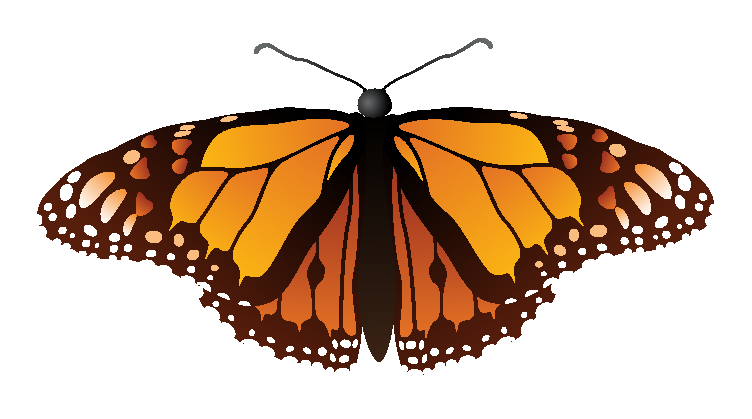
\includegraphics[scale=0.1]{mybutterfly.eps}};
\node at (2,0)
{
\begin{tikzpicture}[scale=0.6]
  \draw[linecolor,xscale=0.8,yscale=0.4,thick] (-4,-4) grid (4,4);
\end{tikzpicture}
};

\node[xscale=2] at (2.3,0.6){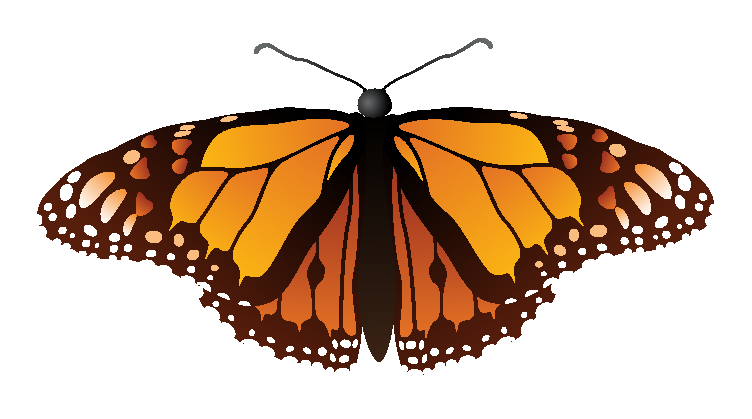
\includegraphics[scale=0.1]{mybutterfly.eps}};
\draw[<->,very thick](0.75,0)--(3.25,0);
\draw[<->,very thick](2,-1.25)--(2,1.25);
\end{tikzpicture}
\end{minipage}\quad
\begin{minipage}{0.45\linewidth}
\centering
\begin{tikzpicture}

\node at (-1.5,0)
{\begin{tikzpicture}[scale=0.6]
  \draw[linecolor,xscale=0.4,yscale=0.4,thick] (-4,-4) grid (4,4);
\end{tikzpicture}
};
\draw[thick,scale=1,<-](1,1) arc (70:110:3cm);
\node[above]at (0,1.2){$f(x,y)=(x+y,y)$};
\draw[<->,very thick](-2.75,0)--(-0.25,0);
\draw[<->,very thick](-1.5,-1.25)--(-1.5,1.25);
\node at (-1.2,0.6){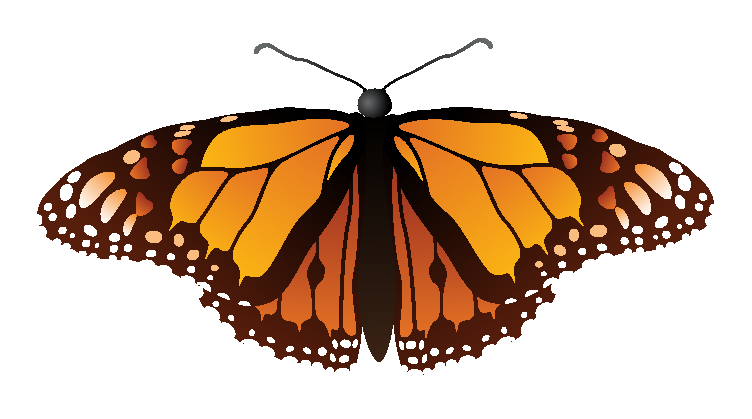
\includegraphics[scale=0.1]{mybutterfly.eps}};
\node at (2,0)
{
\begin{tikzpicture}[scale=0.6]
  \draw[linecolor,xscale=0.6,yscale=0.6,thick] (-4,-4) grid (4,4);
\end{tikzpicture}
};

\node[xscale=2,rotate=-100] at (2.3,0.6){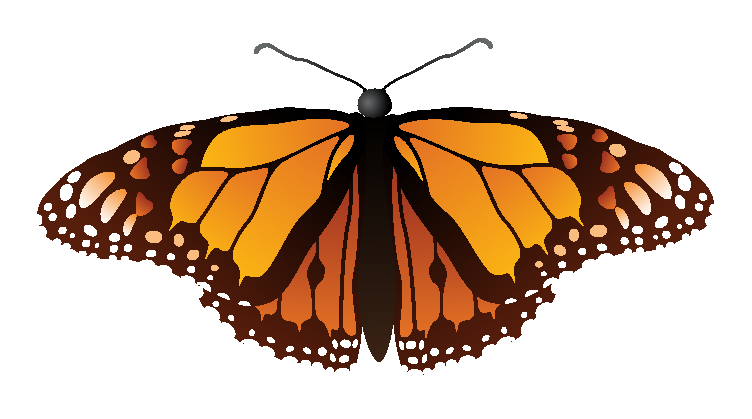
\includegraphics[scale=0.1]{mybutterfly.eps}};
\draw[<->,very thick](0.75,0)--(3.25,0);
\draw[<->,very thick](2,-1.25)--(2,1.25);
\end{tikzpicture}
\end{minipage}



\begin{minipage}{0.45\linewidth}
\centering
\begin{tikzpicture}

\node at (-1.5,0)
{\begin{tikzpicture}[scale=0.6]
  \draw[linecolor,xscale=0.4,yscale=0.4,thick] (-4,-4) grid (4,4);
\end{tikzpicture}
};
\draw[thick,scale=1,<-](1,1) arc (70:110:3cm);
\node[above]at (0,1.2){$f(x,y)=(x+y,x-y)$};
\draw[<->,very thick](-2.75,0)--(-0.25,0);
\draw[<->,very thick](-1.5,-1.25)--(-1.5,1.25);
\node at (-1.2,0.6){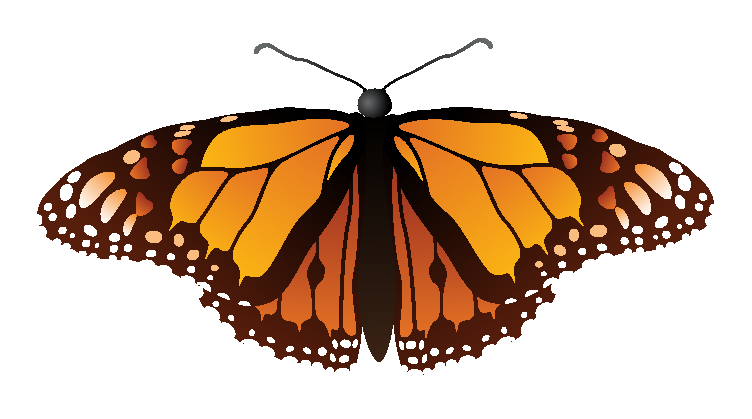
\includegraphics[scale=0.1]{mybutterfly.eps}};
\node at (2,0)
{
  \begin{tikzpicture}[scale=0.6]
  \draw[linecolor,xscale=0.6,yscale=0.6,thick,rotate=45] (-4,-4) grid (4,4);
\end{tikzpicture}
};

\node[xscale=2,rotate=-135] at (2.3,0.6){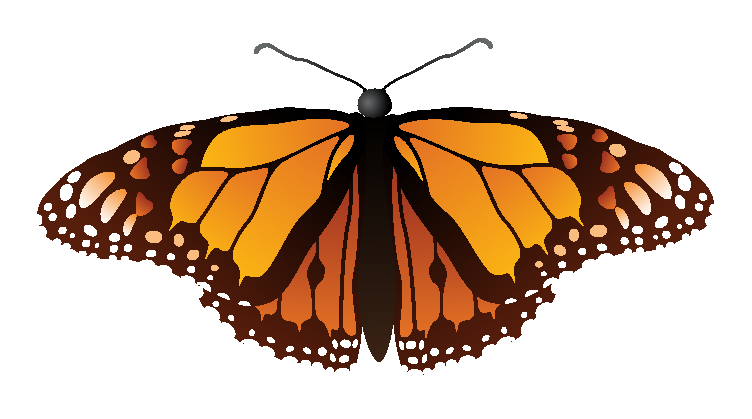
\includegraphics[scale=0.1]{mybutterfly.eps}};
\draw[<->,very thick](0.75,0)--(3.25,0);
\draw[<->,very thick](2,-1.25)--(2,1.25);
\end{tikzpicture}
\end{minipage}\quad
\begin{minipage}{0.45\linewidth}
\centering

\begin{tikzpicture}

\node at (-1.5,0)
{\begin{tikzpicture}[scale=0.6]
  \draw[linecolor,xscale=0.4,yscale=0.4,thick] (-4,-4) grid (4,4);
\end{tikzpicture}
};
\draw[thick,scale=1,<-](1,1) arc (70:110:3cm);
\node[above]at (0,1.2){$f(x,y)=(\frac{2}{3}x-\frac{2}{3}y,\frac{1}{3}x-\frac{1}{6}x)$};
\draw[<->,very thick](-2.75,0)--(-0.25,0);
\draw[<->,very thick](-1.5,-1.25)--(-1.5,1.25);
\node at (-1.2,0.6){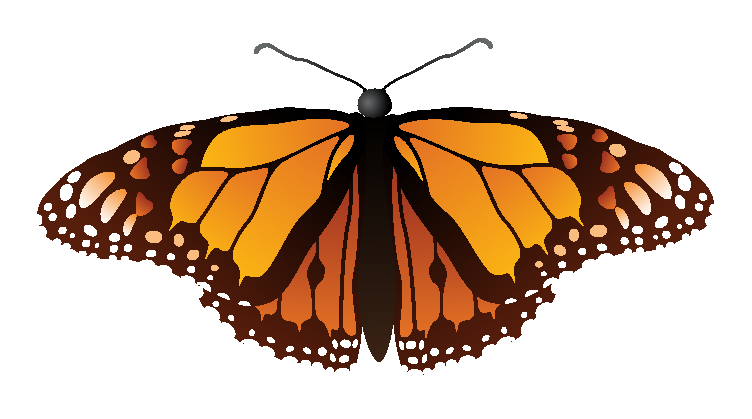
\includegraphics[scale=0.1]{mybutterfly.eps}};
\node at (2,0)
{
\begin{tikzpicture}[scale=0.6]
  \draw[linecolor,xscale=0.8,yscale=0.4,thick] (-4,-4) -- (4,4);
\end{tikzpicture}
};

\node[xscale=2,rotate=90] at (2.3,0.6){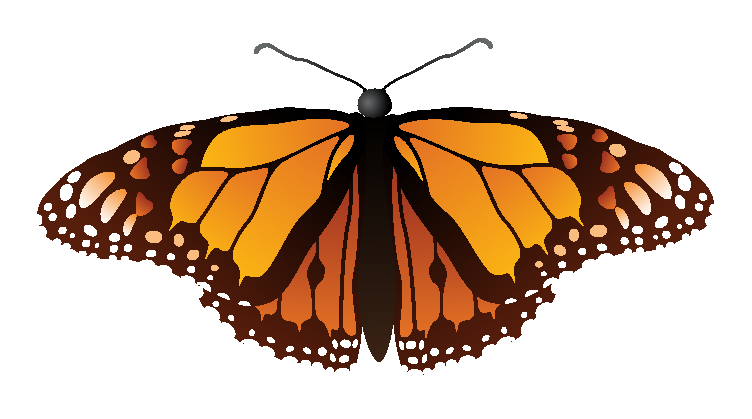
\includegraphics[scale=0.1]{mybutterfly.eps}};
\draw[<->,very thick](0.75,0)--(3.25,0);
\draw[<->,very thick](2,-1.25)--(2,1.25);
\end{tikzpicture}
  \caption{Four linear transformations from $\R^2$ to $\R^2$ \label{fig:four_trans}}
\end{minipage}
\end{figure}

图~\ref{fig:four_trans} 显示从$\R^2$到$\R^2 $线性变换的四个例子。 的转变
图~\ref{fig:four_trans} \textit{scale},\textit{shear},
\textit{旋转/缩放}和\textit{project}。 未显示是\textit{reflection},例如$ f(x,y)=(x,-y)$。 这是
从$ \ R ^ 2 $到
$ \R^2 $可以写成这些变换的组合基本类型。

基于图~\ref{fig:four_trans}我们进行猜想, 线性
转换将等距线映射到等距线,其中重合线等距间隔为零
(如上例所示)。 这几乎是准确的:有时也一样等距的线可以映射到等距的点
(锻炼~\ref{exer:espoints})。 以下定理给出了线性的几何特征。

\begin{theo}{线性变换的等价定理}{equalspacing}
  A function from $\R^2$ to $\R^2$ is linear if and only if it maps
  the origin to the origin and equally spaced lines* to equally spaced
  lines or points. \sidenote{* \textit{Equally spaced lines} are lines
    which are parallel and for which the distances between consecutive
    lines are the same}
\end{theo}

但是,我们还没有完成。 请注意,我们假设从原点到$(a,c)$的线段为从原点到$(b,d)$的线段顺时针旋转。 要是我们
切换这些线段,同样的理由给我们公式$ bc-ad $。 我们可以说所有这些区域转换的因子为$\boxed{|ad-bc|}$。

\begin{exercise}{线性变换定理的应用练习}{exercise}
  Use Theorem~\ref{th:equalspacing} to show that if
  $f : \R^2 \to \R^2$ rotates every point counterclockwise about the
  origin by $30^\circ$, there necessarily exist $a,b,c,d\in\R$ such
  that $f(x,y) = (ax+ by, cx+ dy)$ for all $(x,y) \in\R^2$.
\end{exercise}

我们可以按以下方式解释~\ref{exam:det2}的结果:$ ad-bc $告诉我们$ f(x,y)=(ax + by,cx + dy)$
如何转换区域(通过其绝对值)以及是否将$f$应用于这三个点
$(0,0)$,$(1,0)$和$(0,1)$会反转其方向*(通过标志)。 这个想法很重要,值得它自己的名字。 至
为了简化定义,我们将长度称为$ 1 $维
和面积作为二维体积。 \sidenote{*反转三个点的方向$ A $,$ B $和$ C $表示如果这些点在三角形周围以逆时针顺序给出
   $ ABC $,则它们的图像在三角形周围按顺时针顺序
   它们形成} [-35mm]

\begin{exercise}{线性变换定理的应用}{espoints}
  Show that the linear function $f(x,y)=(2x,0)$ maps any collection of
  equally spaced vertical lines to a collection of equally spaced points.
\end{exercise}

\section{行列式} \label{sec:det}

\sidenote{\href{https://www.youtube.com/watch?v=Ip3X9LOh2dk}{\tbob}
  on the determinant}[-7.5mm]

线性函数从$\R^1$到$\R^1$的斜率它如何扭曲长度。 例如,函数$f(x)= 3x$映射任何间隔
$[a,b]$到间隔$[3a,3b] $的三倍长。 函数$g(x)=-\frac {1}{2} x$将任何间隔映射到
间隔的一半,它也会翻转间隔周围。 可以说线性的斜率的绝对值函数是长度转换所依据的因素,并且
斜率的符号告诉我们函数是否反转实数数字线。

那么,从$\R^2$到$ \R^2$。 我们可以看一下线性变换吗?计算变换扭曲的因数地区? 答案是肯定的!


对于图~\ref{fig:four_trans}中的每个线性变换,图片图像侧的四边形都是
全等。 这表明线性变换确实可以以相同的因子变换每个区域。 根据这个事实,
我们考虑一个正方形的图像就足够了将取为$[0,1]^2 $,这是两个点的坐标集
介于0和1之间。


\begin{example}{}{det2}
  Find the area of the image of the unit square $[0,1]^2$ under the
  transformation
  \[
    f(x,y) = (ax + by, cx + dy).
  \]
  \begin{center}
    \begin{asy}
      size(10cm);
      settings.outformat="pdf";
      draw((0,2)--(0,0)--(2,0),Arrows());
      filldraw(box((0,0),(1,1)),lightgray);
      draw("$1$",(1,0),align=S);
      draw("$1$",(0,1),align=W);
      draw(shift((3,0))*((0,2)--(0,0)--(2,0)),Arrows());
      filldraw(shift((3,0))*((0,0)--(2,1)--(3,2)--(1,1)--cycle),lightgray);
      dot("$(a,c)$",shift((3,0))*(2,1),align=SE);
      dot("$(b,d)$",shift((3,0))*(1,1),align=NW);
    \end{asy}
  \end{center}
\end{example}

\begin{solution}
  The area of the unit square can be calculated by filling in some
  triangles to get a complete rectangle, as follows:
  \begin{center}
    \begin{asy}
      size(6cm);
      draw(((0,2.3)--(0,0)--(3.3,0)),Arrows());
      filldraw(((0,0)--(2,1)--(3,2)--(1,1)--cycle),lightgray);
      dot("$(a,c)$",(2,1),align=2*E);
      dot("$(b,d)$",(1,1),align=2*W);
      dot("$(a+b,c+d)$",(3,2),align=2*E);
      filldraw((0,0)--(3,0)--(2,1)--cycle,LightSeaGreen+opacity(0.5));
      filldraw((0,2)--(1,1)--(3,2)--cycle,LightSeaGreen+opacity(0.5));
      filldraw((0,0)--(1,1)--(0,2)--cycle,LightBlue+opacity(0.5));
      filldraw((3,0)--(2,1)--(3,2)--cycle,LightBlue+opacity(0.5));
    \end{asy}
  \end{center}
  The area of the larger rectangle is $(a+b)(c+d)$, and the total area
  of the triangles we added is
  $2\cdot\tfrac{1}{2} (a+b)(c) + 2\cdot\tfrac{1}{2}
  (c+d)(b)$. Subtracting, we get that the area of the parallelogram is
  $ad - bc$.

  We are not quite finished, however. Note that we assumed in our
  diagram that the line segment from the origin to $(a,c)$ is
  clockwise from the line segment from the origin to $(b,d)$. If we
  switched these line segments around, the same reasoning would have
  given us the formula $bc - ad$. We can put this all together by saying
  that the factor by which areas are transformed is $\boxed{|ad - bc|}$.
\end{solution}

We can interpret the result of Example~\ref{exam:det2} as follows:
$ad - bc$ tells us how $f(x,y) = (ax + by, cx + dy)$ transforms areas
(via its absolute value) and whether applying $f$ to the three points
$(0,0)$, $(1,0)$, and $(0,1)$ reverses their orientation* (via its
sign). This idea is important enough to deserve its own name. To
simplify the definition, we refer to length as $1$-dimensional volume
and area as 2-dimensional volume. \sidenote{* Reversing the
  orientation of three points $A$, $B$, and $C$ means that if these
  points are given in counterclockwise order around the triangle
  $ABC$, then their images are in clockwise order around the triangle
  they form}[-35mm]

\begin{defn}{Determinant }{def:det} \bang{-5mm}
  The \textbf{determinant} of a linear transformation from $\R^n$ to
  $\R^n$ is the signed factor by which it transforms $n$-dimensional
  volumes.
\end{defn}

We have already figured out that the determinant of $f(x) = mx$ from
$\R^1$ to $\R^1$ is the slope $m$, and the determinant of a function
$f(x,y) = (ax + by, cx + dy)$ from $\R^2$ to $\R^2$ is given by the
formula $ad - bc$.

For convenience, we sometimes represent a linear function by arranging
its coefficients into a grid of numbers called a \textit{matrix}. By
convention, rows correspond to coordinates of the output of the
function, and columns correspond to the variables. So, for example,
$f(x,y) = (ax + by, cx + dy)$ is represented by the matrix
$\left[\begin{array}{cc} a & b \\ c & d \end{array}\right]$. So we
have
\[
  {d}et [m] = m, \text{ and} \qquad {d}et \left[\begin{array}{cc} a & b \\ c & d \end{array}\right] = ad - bc.
\]

\begin{exercise}{}{det}
  Find the determinant of each of the following matrices, and draw the
  image of the unit square under the corresponding linear
  transformations to see that the value of the determinant you
  computed makes sense.

  \pairofprobs{$\left[\begin{array}{cc} 1 & 0 \\ 0 & -1 \end{array}\right]$}{
    $\left[\begin{array}{cc} 2 & 1 \\ 0 & 2 \end{array}\right]$}

  \pairofprobs{$\left[\begin{array}{cc} 0 & 1 \\ -1 & 0 \end{array}\right]$}{
    $\left[\begin{array}{cc} 2 & 1  \\ 4 & 2 \end{array}\right]$}
\end{exercise}

We define the determinant of a linear transformation
\[
  f(x,y,z) = (ax + by + cz, \, dx + ey + fz,\, gx + hy  + iz)
\]
to be the product of two quantities:
\begin{enumerate}[(i),topsep=-6pt]
  \item the volume of the three-dimensional shape, called a
    \textit{parallelepiped}, whose vertices are the images under $f$
    of the vertices of the unit cube $[0,1]^3$
    (Figure~\ref{fig:3dlinear}).
  \item a factor of
    $\pm1$ which is equal to $-1$ if and only if the orientation of a
    small loop drawn on a face is reversed (see
    Figure~\ref{fig:3dlinear}), from the point of view of a small
    person standing on the solid with their head pointing toward the
    outside.
\end{enumerate}

\begin{center}
  \begin{asy}
    import three;
    import tube;
    unitsize(1.5cm);
    settings.outformat="pdf";
    draw(O--3*X,Arrow3());
    draw(O--3*Y,Arrow3());
    draw(O--3*Z,Arrow3());
    triple[] A =
    {
      (1,0,0),
      (0,1,0),
      (0,0,1)
    };
    currentprojection=orthographic(4,2,1);
    guide3 p = O--A[0]--A[0]+A[1]--A[1]--cycle;
    draw(p);
    draw(surface(p),0.5*white+0.5*blue+opacity(0.7),nolight);
    guide3 p = O--A[1]--A[1]+A[2]--A[2]--cycle;
    draw(p);
    draw(surface(p),0.7*yellow+opacity(0.7),nolight);
    guide3 p = O--A[2]--A[2]+A[0]--A[0]--cycle;
    draw(p);
    draw(surface(p),0.5*green+opacity(0.7),nolight);
    guide3 p = A[2]--A[2]+A[0]--A[2]+A[0]+A[1]--A[2]+A[1]--cycle;
    draw(p);
    draw(surface(p),0.5*white+0.5*blue+opacity(0.7),nolight);
    guide3 p = A[0]--A[0]+A[1]--A[0]+A[1]+A[2]--A[0]+A[2]--cycle;
    draw(p);
    draw(surface(p),0.7*yellow+opacity(0.7),nolight);
    guide3 p = A[1]--A[1]+A[2]--A[1]+A[2]+A[0]--A[1]+A[0]--cycle;
    draw(p);
    draw(surface(p),0.5*green+opacity(0.7),nolight);
    draw(shift(A[2])*(A[0]/3+A[1]/2 .. A[0]/2+A[1]/4  .. 2*A[0]/3 + A[1]/2),linewidth(3.0),Arrow3(10));
    label("$f(x,y,z) = (x , x + y + z, 2y + z)$",(0,2.5,2.5),fontsize(8));
    draw((0,2,2)..(0,3,2.1)..(0,4,2),Arrow3());
  \end{asy}
  \begin{asy}
    import three;
    import tube;
    unitsize(1.5cm);
    settings.outformat="pdf";
    settings.render=8;
    draw(O--3*X,Arrow3());
    draw(O--3*Y,Arrow3());
    draw(O--3*Z,Arrow3());
    triple[] A =
    {
      (1,1,0),
      (0,1,2),
      (0,1,1)
    };
    currentprojection=orthographic(4,2,1);
    guide3 p = O--A[0]--A[0]+A[1]--A[1]--cycle;
    draw(p);
    draw(surface(p),0.5*white+0.5*blue+opacity(0.7),nolight);
    guide3 p = O--A[1]--A[1]+A[2]--A[2]--cycle;
    draw(p);
    draw(surface(p),0.7*yellow+opacity(0.7),nolight);
    guide3 p = O--A[2]--A[2]+A[0]--A[0]--cycle;
    draw(p);
    draw(surface(p),0.5*green+opacity(0.7),nolight);
    guide3 p = A[2]--A[2]+A[0]--A[2]+A[0]+A[1]--A[2]+A[1]--cycle;
    draw(p);
    draw(surface(p),0.5*white+0.5*blue+opacity(0.7),nolight);
    guide3 p = A[0]--A[0]+A[1]--A[0]+A[1]+A[2]--A[0]+A[2]--cycle;
    draw(p);
    draw(surface(p),0.7*yellow+opacity(0.7),nolight);
    guide3 p = A[1]--A[1]+A[2]--A[1]+A[2]+A[0]--A[1]+A[0]--cycle;
    draw(p);
    draw(surface(p),0.5*green+opacity(0.7),nolight);
    draw(shift(A[2])*(A[0]/3+A[1]/2 .. A[0]/2+A[1]/4  .. 2*A[0]/3 + A[1]/2),linewidth(3.0),Arrow3(10));
  \end{asy}
  \captionof{figure}{A linear transformation from $\R^3$ to $\R^3$ \label{fig:3dlinear}}
\end{center}

The formula for the determinant turns out to be*\sidenote{* The
  \textit{Geometry of Determinants} section of
  \href{http://joshua.smcvt.edu/linearalgebra/book.pdf}{the free
    online book \textit{Linear Algebra}} by Jim Hefferon includes a
  lengthy discussion of $n\times n$ determinants}
\[
  {d}et \left[
    \begin{array}{ccc}
      a & b & c \\ d & e & f \\ g & h & i
    \end{array}
  \right] =
  aei - afh - bdi + bfg + cdh - ceg.
\]
Unlike the formula $ad - bc$ for the $2\times 2$ matrix, this formula
is not easy to memorize. Let's abbreviate ${d}et [ \hphantom{a} ]$ to
$| \hphantom{a}|$ and write this formula as
\[
  \left|\begin{array}{ccc} a & b & c \\ d & e & f \\ g & h & i \end{array}\right| =
  +\hspace{2pt}a \left|\begin{array}{cc} e & f \\  h & i \end{array}\right|
  -b \left|\begin{array}{cc} d & f \\  g & i \end{array}\right|
  +c \left|\begin{array}{cc} d & e \\  g & h \end{array}\right|.
\]
This formula is \textit{still} not easy to memorize, so let's break it
down: each term on the right-hand side includes three factors: (i) a $+1$ or
$-1$ which alternates starting with $+1$, (ii) an entry from the top
row (going from left to right), and (iii) the determinant of the matrix you
get when you remove the row and column of that entry from the original
matrix. These smaller matrices are called \textit{minors}, and this
method of calculating the determinant is called \textbf{expansion by
  minors} along the first row. You can also expand by minors along any
row or column (see Exercise~\ref{exer:det3b} below), but if it's an
even-numbered row or column, then the signs start with $-1$ instead of
$+1$.

\begin{exercise}{}{det3a} \setcounter{subitm}{1}
  Calculate each determinant.

  \pairofprobs{$\left|
      \begin{array}{ccc}
        1 & 2 & 3 \\  0 & 4 & 5 \\ 0 & 0  & 6
      \end{array}\right|$}
  {$\left|
      \begin{array}{ccc}
        -4 & 2 & 1 \\ 5 & 0 & 3 \\ -2 & 1 & 3
      \end{array}\right|$}
\end{exercise}

\begin{exercise}{}{det3b}
  Expand by minors along the first \textit{column} of this matrix, and
  show that you get the same result as when you expand by minors along
  the first row.
  \[
    \left|
      \begin{array}{ccc} -2 & \hphantom{-}1 & \hphantom{-}4 \\
        \hphantom{-}1 & \hphantom{-}1 & \hphantom{-}2 \\ \hphantom{-}2
                            & \hphantom{-}0 & -1
      \end{array}
    \right|
  \]
\end{exercise}

\begin{exercise}{}{det3c}
  Find the values of $t$ for which the determinant of the following matrix is zero.
  \[
    \left|\begin{array}{ccc} -2 & t^2 & 4 \\  3 & 1 & 0 \\ 2 & 0  & -1 \end{array}\right|
  \]
\end{exercise}

\begin{exercise}{}{transpose}
  The \textbf{transpose} $A^T$ of a matrix $A$ is obtained by swapping rows and
  columns. In other words,
  \[
    \left[
      \begin{array}{ccc} a & b & c
        \\ d & e & f
        \\ g & h &i
      \end{array}
    \right]^T
    =
    \left[
      \begin{array}{ccc}
        a & d & g\\ b & e & h \\ c & f & i
      \end{array}
    \right].
  \]
  Show  that ${d}et A = {d}et A^T$.
\end{exercise}

\begin{exercise}{}{singular}
  Show that if two rows of a $3 \times 3$ matrix $A$ are the same,
  then ${d}et A = 0$.
\end{exercise}

\chapter{欧氏向量空间}

\section{向量空间} \label{sec:vectors}

\sidenote{\href{https://www.youtube.com/watch?v=fNk_zzaMoSs}{\tbob}
  on vectors}[-7.5mm]


\begin{wrapfigure}[11]{O}{4cm}
  \begin{asy}
    size(4cm);
    real ep = 0.1;
    draw((1,-ep)--(1,ep));
    label("1",(1,0),align=2.5*S);
    label("1",(0,1),align=2*W);
    draw((-ep,1)--(ep,1));
    draw((2,0)--(0,0)--(0,2),Arrows());
    draw((1/2,1)--(2,2),MidnightBlue,Arrow());
  \end{asy}
  \caption{A vector in $\R^2$\label{fig:arrow}}
\end{wrapfigure}
A \textbf{vector} in $\R^n$ is an arrow from one point in $\R^n$ (the
\textit{tail}) to another (the \textit{head}). See
Figure~\ref{fig:arrow}). The \textbf{length}* of a vector is the
distance from the head to the tail. Two vectors are considered
equivalent if they have the same length and the same direction.
\sidenote{* The length of a vector is also called the
  \textbf{norm} or the \textbf{magnitude} of the vector}

The \textbf{components} of a vector are the coordinates of its head
when it is translated so that its tail is at the origin. In other
words, to find the components of a vector, we subtract each coordinate
of its tail from the corresponding coordinate of the head. The
components of the vector in Figure~\ref{fig:arrow} are
$\langle \frac{3}{2} , 1\rangle$---note that we use the pointy
brackets to distinguish components of a vector from coordinates of a
point.*\sidenote{* Actually, vectors and points kind of \textit{are}
  the same, since they are both specified by an ordered tuple of real
  numbers. The distinction is in how we use them and visualize them,
  although you should be prepared to play fast and loose with this
  distinction at times}
We can calculate the components by subtracting the coordinates of the
tail from the coordinates of the head. Two vectors are equivalent if
and only if their components are the same.


The main things we will do with vectors are (i) add two of them
together and (ii) multiply a vector by a real number (which is called
a \textbf{scalar} in this context). These are
defined componentwise:
\begin{align*}
  \langle u_1, u_2 \rangle  +   \langle v_1, v_2 \rangle
  &= \langle u_1  + v_1, u_2 + v_2\rangle, \text{ and} \\
  c \langle u_1, u_2 \rangle
  &= \langle cu_1, cu_2 \rangle.
\end{align*}
These definitions of vector addition and scalar multiplication
lead to natural geometric interpretations, as shown in
Figures~\ref{fig:vectoradd} and \ref{fig:scalarmultiply}.

\begin{center}
  \begin{minipage}{0.45\textwidth}
    \begin{center}
      \begin{asy}
        size(4cm);
        real n = 4;
        real ep = 0.1*n;
        for(int i=1;i<=n;++i){
          draw((i,0)--(i,n),gray);
          draw((0,i)--(n,i),gray);
        }
        draw((0,n+ep)--(0,0)--(n+ep,0),Arrows());
        draw((0,0)--(3,1),MidnightBlue,Arrow());
        draw((0,0)--0.92*(3,1),MidnightBlue+linewidth(1.5));
        draw((3,1)--(4,3),DarkOrange,Arrow());
        draw((3,1)--(4,3) - 0.08*(1,2),DarkOrange+linewidth(1.5));
        draw((0,0)--(4,3),SeaGreen,Arrow());
        draw((0,0)--0.95* (4,3),SeaGreen+linewidth(1.5));
      \end{asy}
    \end{center}
    \captionof{figure}{Vector addition: $\langle 3,1 \rangle + \langle 1,2
      \rangle = \langle 4,3 \rangle$\label{fig:vectoradd}}
  \end{minipage}
  \begin{minipage}{0.45\textwidth}
    \begin{center}
      \begin{asy}
        size(4cm);
        real n = 4;
        real ep = 0.1*n;
        for(int i=1;i<=n;++i){
          draw((i,0)--(i,n),gray);
          draw((0,i)--(n,i),gray);
        }
        draw((0,n+ep)--(0,0)--(n+ep,0),Arrows());
        draw((0,0)--1.9*(2,1),MidnightBlue+linewidth(2.5));
        draw((0,0)--(4,2),MidnightBlue,Arrow());
        draw((0,0)--(2,1),DarkOrange,Arrow());
        draw((0,0)--0.93*(2,1),DarkOrange+linewidth(1.25));
      \end{asy}
    \end{center}
    \captionof{figure}{Scalar multiplication:
      $2\langle 2,1 \rangle = \langle 4,2
      \rangle$\label{fig:scalarmultiply}}
  \end{minipage}
\end{center}

We typically assign names for vectors which are lowercase boldface
letters, like $\vec{u}$ or $\vec{v}$.  Looking at
Figure~\ref{fig:scalarmultiply}, we make the following observation.

\begin{obs}{Parallel vectors}{vecparallel} \bang{-5mm} Two vectors
  $\vec{u}$ and $\vec{v}$ are parallel if $\vec{u} = c \, \vec{v}$ for
  some scalar $c$.
\end{obs}

Vector operations satisfy several properties suggested by the
notation,* such as commutativity
($\vec{u} + \vec{v} = \vec{v} + \vec{u}$), associativity
($(\vec{u} + \vec{v}) + \vec{w} = \vec{u} + (\vec{v} + \vec{w})$), the
distributive property of scalar multiplication across vector addition
(Exercise~\ref{exer:vector_distribution}) and so on. One simple strategy
for proving such property-verification exercises is to
write out what each side of the equation means in terms of components and
then simplify both sides until it's clear that they are equal. \sidenote{*
  That is, we use the same notation as we use for
  multiplication/addition of real numbers because these operations
  satisfy many of the same properties}[-12mm]

\begin{exercise}{}{vector_distribution}
  Show that scalar multiplication distributes across vector
  addition. In other words, show that for all $c\in \R$ and vectors
  $\vec{u}$ and $\vec{v}$ in $\R^n$, we have
  \[
    c(\vec{u} + \vec{v})= c
    \vec{u} + c \vec{v}.
  \]
\end{exercise}

\begin{exercise}{}{vector_distribution_2}
  Show that scalar multiplication distributes across scalar
  addition. In other words, show that for all $c\in \R$, $d \in \R$, and vectors
  $\vec{u}$ and $\vec{v}$ in $\R^n$, we have
  \[
    (c+d)\vec{u}  = c \vec{u} + d \vec{u}.
  \]
\end{exercise}

\begin{exercise}{}{vector_subtraction}
  Choose two vectors $\vec{u}$ and $\vec{v}$ with small integer
  coordinates and draw a figure to show how $\vec{u}$, $\vec{v}$, and $\vec{u}
  - \vec{v}$
  fit together to form a triangle.
\end{exercise}

\begin{exercise}{}{}
  Suppose that $\mathbf{u}$ and $\mathbf{v}$ are vectors in $\R^2$ or
  $\R^3$, and suppose that $\mathbf{w} = c \mathbf{u} + d \mathbf{v}$,
  where $c$ and $d$ are both in $[0,1]$. If the tail of $\mathbf{w}$
  is at the origin, then what is the set of possible locations for the
  head of $\mathbf{w}$?
\end{exercise}

The following example shows how vector ideas can be applied to geometry
problems.

\begin{example}{}{trianglemidpoint}
  Use vectors to prove that the line segment joining the midpoints of
  two sides of a triangle is parallel to the third side and half its
  length.
\end{example}

\begin{solution}
  \begin{lrbox}{\asybox}
    \begin{asy}
      size(3cm);
      label("$O$",(0,0),align=W);
      label("$A$",(2,1),align=E);
      label("$B$",(1,3),align=N);
      draw((0,0)--(2,1)--(1,3)--cycle);
      draw((0,0)--(2,1),SeaGreen,Arrow());
      draw((0,0)--(1,3),MidnightBlue,Arrow());
      draw((1,1/2)--(1/2,3/2),Arrow());
      label("$\mathbf{u}$",(1,1/2),align=SE,SeaGreen);
      label("$\mathbf{v}$",(1/2,3/2),align=WNW,MidnightBlue);
    \end{asy}
  \end{lrbox}
  \begin{insetfigure}{\usebox{\asybox}}[][4pt]
    Define $\vec{u}$ and $\vec{v}$ to be two vectors with a common
    tail at one vertex $O$ of the triangle and heads at the other two
    vertices $A$ and $B$ as shown. Then the vectors from $O$ to the
    midpoints of $OA$ and $OB$ are $\tfrac{1}{2}\vec{u}$ and
    $\tfrac{1}{2}\vec{v}$, since the midpoint of a line segment is
    defined to be the point which is halfway between the endpoints.

    Therefore, the vector $\vec{w}$ from one midpoint to another is
    $\tfrac{1}{2} \vec{v} - \tfrac{1}{2}\vec{u}$. By the
    distributive property, this is equal to
    $\tfrac{1}{2}(\vec{v} - \vec{u})$. The vector from $A$ to $B$
    is $\vec{v} - \vec{u}$.  Therefore, $\vec{w}$ has the same
    direction as the vector from $A$ to $B$ (by
    Observation~\ref{obs:vecparallel}) and is half as long.
  \end{insetfigure}
\end{solution}

\begin{exercise}{}{}
  Use vectors to show that the diagonals of a parallelogram bisect one
  another.
\end{exercise}

\begin{exercise}{}{}
  A median of a triangle is a line segment from a vertex of the
  triangle to the midpoint of the opposite side. Use vectors to show
  that for any triangle, there is a point on all three medians. (Hint:
  This point will split each median into two segments, one of which is
  twice as long as the other.)
\end{exercise}

\section{向量的点乘} \label{sec:dot}

\sidenote{\href{https://www.youtube.com/watch?v=LyGKycYT2v0}{\tbob}
  on the dot product}[-7.5mm]

The fundamental vector operations of scalar multiplication and vector
addition are not sufficient to capture information about a really important
geometric concept: \textit{angle}. So we introduce a new vector
operation.

\begin{defn}{Dot product}{dotproduct}
  The \textbf{dot product} of two three-dimensional vectors $\vec{u}
  = \langle u_1, u_2, u_3 \rangle$
  and $\vec{v} =  \langle v_1, v_2, v_3 \rangle$ is defined by
  \[
    \vec{u} \cdot \vec{v} = \langle u_1, u_2, u_3 \rangle \cdot
    \langle v_1, v_2, v_3 \rangle = u_1 v_1 + u_2 v_2+ u_3v_3.
  \]
\end{defn}

The dot product distributes across vector addition, and it is closely
related to length, as shown in the following exercise. We denote by
$|\vec{u}|$ the length of $\vec{u}$.

\begin{exercise}{}{dotproduct}
  Verify that $\vec{u} \cdot (\vec{v} + \vec{w}) = \vec{u} \cdot
  \vec{v} + \vec{u} \cdot \vec{w}$ and that $\vec{u} \cdot
  \vec{u} = |\vec{u}|^2$.
\end{exercise}

Now we establish the relationship between the dot product and angle.
\enlargethispage{5mm}

\begin{example}{}{}
  Use the law of cosines to show that $\vec{u} \cdot \vec{v} =
  |\vec{u}| |\vec{v}| \cos\theta$, where $\theta$ is the angle
  between $\vec{u}$ and $\vec{v}$.
\end{example}

\begin{solution}
  \begin{lrbox}{\asybox}
    \begin{asy}
      size(3cm);
      real ep = 0.2;
      draw((0,0)--(2,1)--(1,3)--cycle);
      draw((0,0)--(2,1),Arrow());
      draw((0,0)--(1,3),Arrow());
      draw((1,3)--(2,1),Arrow());
      label("$\theta$",(0.3,0.38));
      label("$\mathbf{u}$",(1,1/2),align=SE);
      label("$\mathbf{v}$",(1/2,3/2),align=WNW);
      label("$\mathbf{u} - \mathbf{v}$",(3/2,2),align=ENE);
    \end{asy}
  \end{lrbox}
  \begin{insetfigure}{\usebox{\asybox}}
    We apply the law of cosines to the triangle with sides
    $\vec{u}$, $\vec{v}$, and $\vec{u} - \vec{v}$. We get
    \[
      |\vec{u} - \vec{v}|^2 =  |\vec{u}|^2 +  |\vec{v}|^2  -2|\vec{u}|
      |\vec{v}|\cos\theta
    \]
    The left-hand side works out to
    \[
      |\vec{u} - \vec{v}|^2 =
      (\vec{u} - \vec{v}) \cdot
      (\vec{u} - \vec{v}) =
      |\vec{u}|^2 + |\vec{v}|^2 - 2\, \vec{u} \cdot
      \vec{v}.
    \]
    Subtracting these equations yields $\vec{u} \cdot \vec{v} =
    |\vec{u}| |\vec{v}| \cos\theta$.
  \end{insetfigure}
\end{solution}

Particularly noteworthy is the case where $\theta$ is a right angle:
We say that two vectors are \textbf{perpendicular} or
\textbf{orthogonal} or  \textbf{normal} if they meet at a right angle.

\begin{obs}{Perpendicular vectors}{} \bang{-5mm}
  Two vectors $\vec{u}$ and $\vec{v}$ are perpendicular if and
  only if $\vec{u} \cdot \vec{v} = 0$.
\end{obs}

The following example shows how we can use the relation
$\vec{u} \cdot \vec{v} = |\vec{u}| |\vec{v}| \cos\theta$ to find an
angle when information about coordinates is available.

\begin{example}{}{}
  Find the angle between the diagonal of a cube and a diagonal of one
  of its faces.
  \begin{center}
    \begin{asy}[width=2cm]
      import three;
      currentlight.background = softblue;
      defaultpen(linewidth(0.8));
      size(5cm);
      currentprojection=orthographic(4,2,1.2);
      draw(box((0,0,0),(1,1,1)));
      draw((0,0,0)--(1,1,0));
      draw((0,0,0)--(1,1,1));
    \end{asy}
  \end{center}
\end{example}

\begin{solution}
  The vector from the origin to the opposite corner of the cube is $\langle
  1,1,1\rangle$. The vector from the origin to the opposite corner of
  the bottom face is $\langle 1,1,0 \rangle$. Therefore, the angle is given by
  \[
    \theta = \cos^{-1}\left(\frac{\mathbf{u} \cdot
        \mathbf{v}}{|\mathbf{u}||\mathbf{v}|}\right) = \cos^{-1}\left(
      \frac{1 + 1 + 0}{\sqrt{1^2 + 1^2 + 1^2}\sqrt{1^2+1^2+0^2}}
    \right) = \boxed{\cos^{-1}\left(\frac{2}{\sqrt{6}}\right)}.
  \]
\end{solution}

\begin{exercise}{}{}
  Sketch the vectors $\mathbf{u} = \langle 4,2 \rangle$ and
  $\mathbf{v} = \langle -1, 2\rangle$ and show geometrically that they
  are perpendicular.

  Then verify that the coordinate formula for dot product indeed gives
  $\mathbf{u} \cdot \mathbf{v} = 0$ for these two vectors.
\end{exercise}

We conclude this section by addressing the out-of-nowhere step where
we defined the formula for the dot product. We could have begun with
the geometric formula
$\vec{u} \cdot \vec{v} = |\vec{u}| |\vec{v}| \cos\theta$ as the
\textit{definition} of the dot product, derived the distributive
property of the dot product across vector addition using geometry, and
then obtained the formula for the dot product in the following
way: define $\vec{i} = \langle1,0,0\rangle$,
$\vec{j} = \langle0,1,0\rangle$, and $\vec{k} =
\langle0,0,1\rangle$. Then a vector
$\vec{u} = \langle u_1, u_2, u_3\rangle$ can be written as
\[
  \vec{u} = u_1 \vec{i} + u_2 \vec{j} + u_3 \vec{k},
\]
and similarly for $\vec{v}$. Then
\begin{align*}
  \vec{u} \cdot \vec{v} &= (u_1 \vec{i} + u_2 \vec{j} + u_3
                          \vec{k})(v_1 \vec{i} + v_2 \vec{j} + v_3 \vec{k})  \\
                        &= u_1 v_1 \vec{i} \cdot \vec{i} + u_1 v_2 \vec{i} \cdot
                          \vec{j}  + u_1 v_3 \vec{i} \cdot \vec{k}  + \\
                        &\hspace{5mm}  u_2 v_1 \vec{j} \cdot \vec{i} + u_2 v_2 \vec{j} \cdot
                          \vec{j}  + u_2 v_3 \vec{j} \cdot \vec{k}  + \\
                        &\hspace{5mm}  u_3 v_1 \vec{k} \cdot \vec{i} + u_3 v_2 \vec{k} \cdot
                          \vec{j}  + u_3 v_3 \vec{k} \cdot \vec{k},
\end{align*}
by the distributive property. This looks like a mess, but since
$\vec{i}$,  $\vec{j}$, and  $\vec{k}$ are
perpendicular, six of these nine terms are zero. Furthermore, since
$\vec{i}\cdot \vec{i} = 1$ and similarly for $\vec{j}$ and
$\vec{k}$, we end up with $  \vec{u} \cdot \vec{v}  = u_1 v_1
+ u_2 v_2 + u_3 v_3$, as desired.

\begin{exercise}{}{}
  Show that the vectors
  $\mathbf{u} = \langle \cos \theta, \sin \theta \rangle$ and
  $\mathbf{v} = \langle -\sin \theta, \cos \theta \rangle$ are unit
  vectors (meaning that the length of each is 1). Show that $\vec{u}$
  and $\vec{v}$ are orthogonal.
\end{exercise}

\begin{exercise}{Orthogonal Projection}{proj}
  Suppose vectors $\vec{u}$ and $\vec{v}$ are given with
  $|\mathbf{u}| = 1$. If $\vec{v} = \vec{v}_1 + \vec{v_2}$, where
  $\vec{v}_1$ and $\vec{v}_2$ are perpendicular and $\vec{v}_1$ is
  parallel to $\vec{u}$, then $\vec{v}_1$ is called the
  \textit{orthogonal projection} of $\vec{v}$ onto $\vec{u}$. The
  magnitude of $\mathbf{v}_1$ is called the \textit{component} of
  $\mathbf{v}$ in the $\mathbf{u}$ direction.

  \begin{enumerate}[(a)]
  \item Draw a figure illustrating the relationship between $\vec{u}$,
    $\vec{v}$, $\vec{v}_1$, and $\vec{v}_2$.

  \item Use right-triangle trigonometry to find a formula for the
    length of $\mathbf{v}_1$ in terms of the angle $\theta$ between
    $\vec{u}$ and $\vec{v}$, and then use dot products to find a
    formula for $\vec{v}_1$ in terms of $\vec{u}$ and $\vec{v}$.

  \item Use your findings to support the statement \textit{dotting
      with a unit vector $\mathbf{u}$ gives the component in the
      $\mathbf{u}$ direction}.
  \end{enumerate}
\end{exercise}

\section{向量的叉乘} \label{sec:cross}

\sidenote{\href{https://www.youtube.com/watch?v=eu6i7WJeinw}{\tbob}
  on the cross product}[-7.5mm]

In the last section we introduced a vector product which reveals
information about \textit{angle}; in this section we'll see a new
vector product which gives us information about \textit{area}.

\begin{wrapfigure}[8]{O}{4cm}
  \begin{asy}[width=4cm]
    import three;
    import tube;
    unitsize(1.5cm);
    currentprojection=perspective(7.46, 2.9, 0.72);

    draw(O--3*X,Arrow3());
    draw(O--3*Y,Arrow3());
    draw(O--3*Z,Arrow3());

    triple u = (1,0.75,-0.5);
    triple v = (0,2,1);
    triple w = cross(u,v) ;

    real eps = 0.05;

    draw(eps*w -- eps*w + eps*(v+u) -- eps*(v+u));

    draw(O--u,Arrow3());
    draw(O--v,Arrow3());
    draw(O--w,Arrow3());

    label("$\mathbf{u}$",0.5*u,align=SW);
    label("$\mathbf{v}$",0.5*v,align=N);
    label("$\mathbf{u}\times \mathbf{v}$",1.1*w,align=E);

    draw(surface(O--u--u+v--v--cycle),LightSeaGreen+opacity(0.4));
  \end{asy}
  \caption{The cross product of $\mathbf{u}$ and $\mathbf{v}$, whose
    length is equal to the area of the parallelogram shown \label{fig:crossprod}}
\end{wrapfigure}

The \textbf{cross product} of $\mathbf{u} = (u_1,u_2,u_3)$ and
$\mathbf{v} = (v_1,v_2,v_3)$ is defined by expanding the following
`determinant' by minors along the first row:* \sidenote{* We put
  \textit{determinant} in scare quotes because the matrix entries are
  not numbers}
\sidenote{\href{https://www.youtube.com/watch?v=BaM7OCEm3G0}{\tbob} A
  beautiful explanation of this formula}[20mm]
\[
  \mathbf{u} \times \mathbf{v} =
  \left|
    \begin{array}{ccc}
      \mathbf{i} & \mathbf{j} & \mathbf{k} \\
      u_1 & u_2 & u_3 \\
      v_1 & v_2 & v_3
    \end{array}
  \right| =
  (u_2v_3 - u_3 v_2) \mathbf{i}
  - (u_1 v_3 - u_3 v_1) \mathbf{j}
  + (u_1v_2 - u_2 v_1) \mathbf{k}.
\]

Note that the dot product of two vectors is a scalar, while the cross
product of two vectors is another vector. It turns out that this
vector is orthogonal to \textit{both} of the first two.

\begin{example}{}{}
  Confirm that $\mathbf{u} \times \mathbf{v}$ is orthogonal to
  $\mathbf{u}$ and to $\mathbf{v}$.
\end{example}

\begin{solution}
  We compute $\mathbf{u} \cdot (\mathbf{u} \times \vec{v})$ as
  follows:
  \begin{align*}
    \langle u_1, u_2, u_3 \rangle \cdot \langle u_2v_3 - u_3 v_2,
    - (u_1 v_3 - u_3 v_1),
    u_1v_2 - u_2 v_1 \rangle&= \\
    ( u_2v_3 - u_3 v_2)u_1 &- (u_1 v_3 - u_3 v_1) u_2 +
                             ( u_1v_2 - u_2 v_1) u_3   = 0.
  \end{align*}
  This implies that $\mathbf{u} \times \mathbf{v}$ is orthogonal to
  $\mathbf{u}$. Swapping out $\mathbf{u}$ for $\mathbf{v}$, we see
  that $\mathbf{u} \times \mathbf{v}$ is orthogonal to
  $\mathbf{v}$ too.

  Alternatively, we could note that
  \[
    \mathbf{u} \cdot (\mathbf{u} \times \vec{v}) =
    \left|
      \begin{array}{ccc}
        u_1 & u_2 & u_3 \\        u_1 & u_2 & u_3 \\
        v_1 & v_2 & v_3 \\
      \end{array}
    \right|
  \]
  and conclude using Exercise~\ref{exer:singular} that this
  determinant equals zero.
\end{solution}

\begin{lrbox}{\asybox}
  \begin{asy}[width=1.5cm]
    import olympiad;
    defaultpen(fontsize(4)+linewidth(0.5));
    size(5cm);
    pair A = (1.5,0); pair B = (1,0.85); pair O = (0,0);
    draw(O--A--A+B--B--cycle);
    real eps = 0.1;
    draw((1-eps,0)--(1-eps,eps)--(1,eps));
    draw(B--O--A,linewidth(0.8));
    label("$a$",A/2, align=S);
    label("$b$",B/2, align=NW);
    label(rotate(-90)*"$b\sin\theta$",(1,B.y/2),align=E);
    draw(B--(1,0));
    draw(anglemark(A,O,B,6));
    label("$\theta$",(0.45,0.16));
  \end{asy}
\end{lrbox}

The following exercise provides the advertised connection to
area. Recall from geometry that the area of a parallelogram with sides
of length $a$ and $b$ meeting at an angle $\theta$ is equal to $ab\sin
\theta$.*
\sidenote{* Proof: \usebox{\asybox}}

\begin{exercise}{}{}
  Verify that $|\mathbf{u} \times \mathbf{v}|^2 =
  |\mathbf{u}|^2|\mathbf{v}|^2 - (\mathbf{u}\cdot \mathbf{v})^2$. Use this fact to
  show that
  \[
    |\mathbf{u} \times \mathbf{v}| = |\mathbf{u}||\mathbf{v}|\sin\theta,
  \]
  where $\theta$ is the angle between $\mathbf{u}$ and $\mathbf{v}$.
\end{exercise}

So to sum up: $\mathbf{u} \times \mathbf{v}$ is a vector which is
orthogonal to both $\mathbf{u}$ and $\mathbf{v}$ and whose length is
equal to the area of the parallelogram spanned by $\mathbf{u}$ and
$\mathbf{v}$. Note that there are only two vectors satisfying both of
these conditions. To determine which one is
$\mathbf{u} \times \mathbf{v}$, we use the \textit{right-hand rule}:
imagine orienting your right hand so that you can curl your fingers
from $\mathbf{u}$ towards $\mathbf{v}$. The direction of your thumb
(if it's orthogonal to your fingers) is the direction of
$\mathbf{u} \times \mathbf{v}$.

\begin{exercise}{}{}
  Find the volume of the parallelepiped spanned by
  $\langle 3,4,1 \rangle$,  $\langle -2,4,0 \rangle$, and
  $\langle -5,5,2 \rangle$. (Hint: first find the area of the base,
  then figure out how to use dot products to find the height.)
\end{exercise}

\begin{exercise}{Cross product distributive property}{}
  Show that $\vec{u} \times (\vec{v} + \vec{w}) = \vec{u}\times
  \vec{v} + \vec{u} \times \vec{w}$, if $\vec{u}, \vec{v}$, and
  $\vec{w}$ are vectors.
\end{exercise}

\chapter{R$^{3}$ 空间上的几何}

\section{线与平面} \label{sec:lines_and_planes}

There are various ways to describe a line in 2D space using an
equation, including point-slope form and $y$-intercept form. In this
section we will learn the 3D analogue: equation descriptions of lines
and planes in space. We begin with an example.

\begin{example}{}{line}
  Describe the line $L$ in $\R^3$ passing through the points
  $A = (3,-4,1)$ and $B = (2,-1,4)$.
\end{example}

\begin{solution}
  We can tell whether a given point $(x,y,z)$ in $\R^3$ is on the line
  $L$ using vectors: $(x,y,z)$ is on $L$ if and only if the vector
  from $(3,-4,1)$ to $(x,y,z)$ is a scalar multiple of the vector from
  $(3,-4,1)$ to $(2,-1,4)$ (see Figure~\ref{fig:linecheck}). We can
  turn this into an equation: a point $(x,y,z)$ is on $L$ if and only
  if there exists $t\in \R$ such that
  \[
    t \big\langle 2-3, -1-(-4), 4-1\big\rangle = \big\langle x - 3, y -(-4), z -
    1\big\rangle.
  \]
  Setting components equal, we find that $(x,y,z)$ is on $L$ if and
  only if there exists $t$ so that
  \begin{align} \nonumber
    x &= 3 - t, \\ \label{eq:par}
    y &= -4 + 3t, \text{ and} \\  \nonumber
    z &= 1 + 3t.
  \end{align}
\end{solution}

\begin{wrapfigure}[14]{O}{6cm}
  \begin{asy}
    import tube;
    unitsize(0.5cm);

    currentprojection=perspective(13.1,12.4,4.1);

    draw(O--6*X,Arrow3());
    draw(O--6*Y,Arrow3());
    draw(O--6*Z,Arrow3());

    triple u = (3,-4,1);
    triple v = (2,-1,4);
    triple z = (2.3,-2,1.5);
    dot(u); dot(v); dot(z);

    draw(u + -1*(v-u)--v + (v-u),Arrows3());
    draw(u--z,linewidth(1.2),Arrow3(10));
    draw(u--v,linewidth(1.2),Arrow3(10));

    label("$(x,y,z)$",z,align=E);
    label("$A$",u,align=NW);
    label("$B$",v,align=NW);
  \end{asy}
  \caption{Checking whether $(x,y,z)$ is on the line through $A$ and
    $B$ \label{fig:linecheck}}
\end{wrapfigure}

Note that the solution above involves a new variable $t$; this is
called a \textit{parameter}, and the form we gave as an answer is
called \textbf{parametric form}. You can imagine drawing the line by
starting with $t = 0$, so that your pen begins at $A$, and then
sweeping $t$ through the values from 0 to 1, changing the location
of your pen according to the parametric equations \eqref{eq:par}. Your
pen will sweep out the line segment from $A$ and $B$. Then you can
let $t$ vary beyond 1 to get the rest of the ray past $B$, and you can
let $t$ vary over the negative numbers to get the part of the line on
the other side of $A$.

If we didn't want to involve $t$, note that we could solve for $t$ in
one equation and substitute into the other two, thereby obtaining
\textit{two} equations involving $x$, $y$, and $z$. This makes sense:
starting from the plane, imposing one equation on $x$ and $y$ cuts the
dimension down by one and gives a line. However, starting from 3D
space, we need to reduce the dimension by \textit{two}. So we need
two equations.

The procedure developed in Example~\ref{exam:line} works in general:
the line through $A = (a,b,c)$ and $B$ has parametric form*
\sidenote{* Note that this representation is not unique, since we
  could've used $B$ (or any other point on the line) in place of $A$}
\begin{align*}
  x &= a + v_1 t, \\
  y &= b + v_2 t \\
  z &= c + v_3 t,
\end{align*}
where $\langle v_1, v_2, v_3 \rangle = \overrightarrow{AB}$ is the
vector from $A$ to $B$.

\begin{example}{}{planeequation}
  Describe the plane $P$ passing through the points $A = (1,0,0)$, $B =
  (0,1,1)$, and $C = (0,0,2)$.
\end{example}

\begin{solution}
  We can tell whether $(x,y,z)$ is on $P$ using vectors. Define
  $\mathbf{u}$ and $\mathbf{v}$ to be the vectors from $A$ to $B$ and
  from $A$ to $C$, respectively.
  \begin{center}
    \begin{asy}
      unitsize(1.5cm);
      import three;
      currentlight.background = softyellow;

      draw(O--3*X,Arrow3(5));
      draw(O--3*Y,Arrow3(5));
      draw(O--3*Z,Arrow3(5));

      triple A = (1,0,0);
      triple B = (0,1,1);
      triple C = (0,0,2);
      triple D = (1,-1,2);

      dot("$A$",A,align=SE);
      dot("$B$",B);
      dot("$C$",C);

      draw("$\mathbf{n}$",A--A+cross(B-A,C-A),Arrow3(),align=SW);
      real eps = 0.1;

      draw(A + eps*cross(B-A,C-A) --
      A + eps*cross(B-A,C-A) + eps*(A-C) --
      A + eps*(A-C));

      draw(A--D,Arrow3());
      dot("$(x,y,z)$", D,align=NW);

      draw(surface(A+C-B+0.5*(A-B)--
      A+B-C+0.5*(A-B)--
      B+B-A--
      C+C-A--
      cycle),LightSeaGreen+opacity(0.5));
      draw("$\mathbf{u}$",A--B,Arrow3(),align=SE);
      draw("$\mathbf{v}$",A--C,Arrow3(),align=W);
    \end{asy}
  \end{center}
  If we can find a vector $\mathbf{n}$ which is orthogonal to $P$,
  then we can say $(x,y,z)$ is on $P$ if and only if the vector from
  $A$ to $(x,y,z)$ is orthogonal to $\mathbf{n}$. But we can take
  $\mathbf{n} = \mathbf{u} \times \mathbf{v}$, since the cross product
  of two vectors is orthogonal to both of them. So
  \[
    \mathbf{n} = \langle -1,1, 1\rangle \times \langle -1, 0, 2 \rangle =
    \langle 2,1,1 \rangle.
  \]
  Now we can say that $(x,y,z)$ is on $P$ if and only if* \sidenote{*
    Note that we
    could use $B$ or $C$ instead $A = (1,0,0)$ here and we'd get the same
    equation for the plane}
  \[
    \mathbf{n} \cdot \langle x - 1 , y - 0 , z - 0 \rangle = 0,
  \]
  which simplifies to $\boxed{2x + y + z = 2}$.
\end{solution}

\begin{obs}{Vector normal to a plane}{} \bang{-3mm}
  A vector $\mathbf{n}$ normal to the plane $ax +by + cz = d$
  can be read off from the coefficients:
  \[
    \mathbf{n} = \langle a,b,c \rangle.
  \]
\end{obs}

One important 3D geometry problem is to find distances between points,
lines, and planes.* We define the distance between two sets to be the
\textit{minimum} distance between any pair of points from the
respective sets. \sidenote{* We can ask about the distance from a point to a
  point, a point to a line, a point to a plane, a line to a line, a
  line to a plane, or a plane to a plane}

\begin{example}{}{}
  Consider the line $\ell$ given by the parametric equation
  $(x,y,z) = (1-2t,3,t)$. Find the distance from $\ell$ to the line
  $m$ which is parallel to $\ell$ and which passes through the point
  $(9,4,1)$.
\end{example}

\begin{solution}
  \begin{minipage}[b]{0.65\textwidth}
    The parametric equations give us convenient access to
    a point on each of the two lines as well as a vector $\mathbf{v}$
    which is parallel to both lines. So we make a figure with this
    information.

    If we define $\mathbf{u}$ to be the vector from connecting the two
    given points, we can see by applying right-triangle trigonometry to
    the figure that the desired distance $d$ is equal to
    $|\mathbf{u}| \sin \theta$. Therefore,
    \[
      d = \frac{|\mathbf{u}||\mathbf{v}|\sin \theta}{|\mathbf{v}|} =
      \frac{|\mathbf{u} \times \mathbf{v}|}{|\mathbf{v}|} =
      \frac{\sqrt{105}}{\sqrt{5}} = \boxed{\sqrt{21}}\,.
    \]
  \end{minipage} \:
  \begin{minipage}[b]{0.32\textwidth}
    \begin{asy}[width=5cm]
      import graph;
      defaultpen(fontsize(8));

      real f(real x){
        return x*x;
      }

      pair A = (0,0);
      pair B = (2,1);
      pair C = (-1,1);

      draw(A--B,Arrows());
      draw(A+C--B+C,Arrows());

      dot("$(1,3,0)$",A + 0.2*(B-A),align=2*SSE);
      dot("$(9,4,1)$",C + 0.8*(B-A),align=1.2*WNW);

      draw(A + 0.6*(B-A) -- A + 0.6*(B-A) + 0.6*(-1,2));

      draw("$\mathbf{u}$",A + 0.2*(B-A) -- C + 0.8*(B-A),linewidth(1.0),Arrow(6));
      draw("$\mathbf{v}$",A + 0.2*(B-A) -- A + 0.4*(B-A),linewidth(1.0),Arrow(6),align=3.7*NE);

      label("$\theta$",(A + 0.2*B-A), align=NNE + NE);

      label(rotate(-63)*"$|\mathbf{u}|\sin
      \theta$",(1.13,1.41),align=SW);
    \end{asy}
  \end{minipage}
\end{solution}

Note the basic strategy: (i) draw a figure containing the information
that the problem gives us (a schematic diagram suffices; there is no
need to make it particularly precise), (ii) use right triangle
trigonometry to express the desired distance terms of vectors we have,
and (iii) use vector formulas to calculate the desired quantity using
a dot or cross product.

A second important operation is finding points of intersection.

\begin{example}{}{}
  Find the point where the line $\langle 3 + t, -2t , 3 \rangle$
  intersects the plane $x + y + z = 7$.
\end{example}

\begin{solution}
  A point is on the intersection of two graphs if and only if it's on
  both graphs. Therefore, we're looking for a point $(x,y,z)$ that
  satisfies $x + y + z = 7$ and has the property that there exists
  $t\in \R$ such that $x = 3 + t, y = -2t,$ and $z=3$. Thus we have
  four equations and four unknowns ($x,y,z,t$), and we can substitute
  the last three equations into the first to find that $6-t = 7$,
  which implies $t = -1$. Therefore, the point of intersection is
  $(2,2,3)$.
\end{solution}

\begin{exercise}{}{}
  Find the equation of the plane passing through the points $(1,0,0)$,
  $(0,1,0)$, and $(0,0,1)$. Find the distance from that plane to the
  origin.
\end{exercise}

\begin{exercise}{}{}
  Find the distance between the planes $x+y-2z = 3$ and $x+y-2z = 0$.
\end{exercise}

\begin{exercise}{}{}
  Find the distance between the lines $(x,y,z) = (2t, 1-t, 4)$ and
  $(x,y,z) = (1 + t, -2t, -1-t)$. Hint: these lines are \textit{skew},
  meaning that they are not parallel but do not intersect. Begin by
  using a cross product to find a vector which is perpendicular to
  both lines.
\end{exercise}

\begin{exercise}{}{}
  Describe parametrically the intersection of the planes $2x + z = 3$
  and $x + y - 2z = 4$.
\end{exercise}

\section{向量值函数} \label{sec:motion_in_space}

\subsection{空间上的路径}

Consider a particle moving along the number line in such a way that
its position at time $t$ is given by $r(t)$. Then the velocity of the
particle at time $t$ is given by the first derivative $v(t) =
r'(t)$. The velocity specifies the \textit{speed} of the particle as well as
its \textit{direction} (left if negative, right if positive).

The same is true of a particle moving in 2D or 3D space: its location
is specified by a function customarily denoted $\mathbf{r}(t)$ from
$\R$ to either $\R^2$ or $\R^3$, and its derivative*
$\mathbf{v}(t) = \mathbf{r}'(t)$ at time $t$ tells us the speed of the
particle at that time (via its length) as well as the direction. We
call $\mathbf{r}$ a \textit{path}*. \sidenote{* The derivative of a
  path $\mathbf{r}$ is the vector obtained by taking the derivative of
  each component}[-3cm] \sidenote{* For a function from $\R^1$ to
  $\R^2$ or $\R^3$ to count as a path, we require that each of its
  components be continuous. For example, $\mathbf{r}(t) = (\e^t, t^2 \sin
  t)$ is a path}


\begin{example}[breakable]{}{can}
  Consider a bug which crawls counterclockwise around a cylinder of
  radius 1 meter from
  $(1,0,0)$ to $(1,0,1)$ as shown:
  \begin{center}
    \begin{asy}
      import graph3;
      size(4cm);

      currentprojection=perspective(5.7,3.1,1.26);
      currentlight.background = softblue;

      draw(O--1.4*X,Arrow3());
      draw(O--1.4*Y,Arrow3());
      draw(O--1.2*Z,Arrow3());

      triple f(real t){
        return (cos(2*pi*t), sin(2*pi*t), t);
      }

      path3 g = graph(f,0,1);

      draw(unitcylinder, surfacepen = material(diffusepen=0.4*LightSeaGreen+0.6*black,
      emissivepen=0.4*LightSeaGreen+0.6*black));
      draw(g,DarkRed+linewidth(1.5));

      real t = 0.1;
      draw(f(t) -- f(t) + 0.10 * (-2*pi*sin(2*pi*t), (2*pi)*cos(2*pi*t), 1),DarkBlue+linewidth(1.2),Arrow3(5));
      label("$\mathbf{v}(t)$", f(t+0.065) + 0.2*(cos(0.1),sin(0.1),1) + 0.00 * Z,DarkBlue);
      dot(f(0.11),DarkBlue);
      label("$\mathbf{r}(t)$",(0,1.3,0.4),DarkRed);
    \end{asy}
  \end{center}
  Assuming the bug moves at constant speed and makes the whole journey
  in one second, find a formula for the position and velocity of the
  bug at time $t$.
\end{example}

\begin{solution}
  We can see that the $z$-coordinate of the bug's position increases
  at a constant rate from 0 to 1 as $t$ goes from 0 to 1, so the
  $z$-coordinate of $\mathbf{r}(t)$ is $t$.

  For the $x$ and $y$ coordinates, we need a pair of functions
  $(x(t),y(t))$ that traces out the unit circle in one second. Recall
  that cosine and sine are defined to be the functions that trace out
  the unit circle according to angle, so we can scale them so they
  make it around in 1 second instead of $2\pi$ seconds:
  \[
    (x(t),y(t)) = \left( \cos 2\pi t, \sin 2\pi t
    \right).
  \]
  So all together we have
  \[
    \boxed{\mathbf{r}(t) =  \left\langle \cos 2\pi t, \sin 2\pi t
        , t \right\rangle}\,,
  \]
  which means that
  \[
    \boxed{\mathbf{v}(t) = \left\langle -2\pi \sin 2\pi t, 2\pi\cos 2\pi t
        , 1 \right\rangle}\,.
  \]
\end{solution}

\begin{exercise}{}{}
  Find the times $t \geq 0$ when a particle whose location at time $t$
  is $\mathbf{r}(t) = \langle t^3 - t^2, t\rangle$ is at its slowest.
\end{exercise}

\begin{exercise}{}{}
  The acceleration $\mathbf{a}(t)$ of a particle whose position at
  time $t$ is given by $\mathbf{r}(t)$ is defined to be
  $\mathbf{v}'(t) = \mathbf{r}''(t)$.  Suppose that the acceleration
  $\mathbf{a}(t)$ of a particle is given by
  $\mathbf{a}(t) = \langle 2t, t^2 \rangle$. If
  $\mathbf{r}(0) = \mathbf{0}$ and
  $\mathbf{v}(0) = \langle 1, 2 \rangle$, then find a formula for
  $\mathbf{r}(t)$.
\end{exercise}

\begin{exercise}{}{}
  An astronaut is using a rope to move in space in such a way that his
  position at time $t$ is given by
  $\mathbf{r}(t) = (2+t) \mathbf{i} + (2+\ln t) \mathbf{j} + \left( 7
    - \frac{4}{t^2+1}\right) \mathbf{k}$. The coordinates of the space
  station doorway are $(5,4,9)$. When should the astronaut let go of the
  rope so as to drift into the doorway?
\end{exercise}

Given a curve in $\R^n$, a path $\mathbf{r}$ that traces it out is
called a parametric equation for the curve. \enlargethispage{1cm}

\begin{example}{}{}
  \begin{lrbox}{\asybox}
    \begin{asy}
      size(3cm);
      import graph3;

      real h = 1.5;
      triple[] axes = new triple[] {X, Y, Z};
      for(int i=0; i<axes.length; ++i){
        draw(O--h*axes[i],Arrow3());
      }

      currentlight.background = softblue;
      currentprojection = perspective(4,2,2);

      draw(unitsphere,material(diffusepen=SeaGreen,specularpen=0.2*white,emissivepen=0.35*white));
      draw(surface(new triple(pair p) {real x=p.x, z=p.y; return (x,1-z,z);},
      (-0.2,-0.2),(1.2,1.2)),
      MidnightBlue+opacity(0.5),MidnightBlue);

      draw(graph(new triple(real t) {return (1/sqrt(2)*cos(t),
        1/2 - 1/2*sin(t),
        1/2+1/2*sin(t));},0,2*pi));
    \end{asy}
  \end{lrbox}
  \begin{insetfigure}{\usebox{\asybox}}
    Find a parametric equation describing the intersection of the sphere
    \[x^2 + y^2 + z^2 = 1\]
    and the plane \[y + z = 1.\]
  \end{insetfigure}
\end{example}

\begin{solution}
  \begin{lrbox}{\asybox}
    \begin{asy}
      size(5cm);
      import graph3;
      currentlight.background = softyellow;
      defaultpen(fontsize(6));

      real h = 1.5;
      triple[] axes = new triple[] {X, Y, Z};
      for(int i=0; i<axes.length; ++i){
        draw(O--h*axes[i],Arrow3());
      }

      currentprojection = perspective(4,1.6,2);

      draw(surface(new triple(pair p) {real x=p.x, z=p.y; return (x,1-z,z);},
      (-1.0,-0.2),(1.2,1.2)),
      MidnightBlue+opacity(0.5),MidnightBlue);

      draw(graph(new triple(real t) {return (1/sqrt(2)*cos(t),
        1/2 - 1/2*sin(t),
        1/2+1/2*sin(t));},0,2*pi),MidnightBlue+linewidth(0.7));

      draw(graph(new triple(real t) {return (1/sqrt(2)*cos(t),
        0,
        1/2+1/2*sin(t));},0,2*pi),DarkRed+linewidth(0.7));
      draw(surface(new triple(pair p) {
        real y = p.x, t = p.y;
        return (1/sqrt(2)*cos(t),
        y,
        1/2+1/2*sin(t));},
      (-1,0),(1.15,2*pi),Spline),opacity(0.4)+red,red);

      label("$y + z = 1$",h*Z,MidnightBlue,align=2*E);
      label("$x^2 + 2z^2 - 2z = 0$",0.3*h*X-0.2*Y,DarkRed,align=W);
    \end{asy}
  \end{lrbox}
  \begin{insetfigure}{\usebox{\asybox}}
    The main idea is to reduce the 3D problem to a 2D problem by finding
    a shadow of the curve that we can parameterize. Looking at the
    figure, it appears that the shadow of this curve in the $xz$
    plane is an ellipse. If we substitute $y = 1-z$ into
    $x^2 + y^2 + z^2 = 1$, we see that every point on the curve indeed
    satisfies* $x^2 + 2z^2 - 2z = 0$. \sidenote{* This equation
      describes an elliptical \textit{cylinder}, because it is the set of all
      points whose shadow in the $xz$-plane is in the red ellipse
      shown in the figure}

    Completing the square to get this equation in standard form, we get
    \[
      2x^2 + 4\left(z - \tfrac{1}{2}\right)^2  = 1.
    \]
  \end{insetfigure}

  The intersection of this surface with the $xz$-plane is an ellipse
  which can be parameterized as
  \[
    \left(\tfrac{1}{\sqrt{2}}\cos t, 0, \tfrac{1}{2} + \tfrac{1}{2}\sin t\right),
  \]
  where $t$ ranges over $[0,2\pi]$. Using the equation $y = 1- z$, we
  see that the point on the curve whose shadow is
  $\left(\tfrac{1}{\sqrt{2}}\cos t, 0, \tfrac{1}{2} + \tfrac{1}{2}\sin t\right)$
  is
  $\left(\tfrac{1}{\sqrt{2}}\cos t, \tfrac{1}{2} - \tfrac{1}{2} \sin t,
    \tfrac{1}{2} + \tfrac{1}{2}\sin t\right)$. As $t$ ranges
  from $0$ to $2\pi$, this point goes all the way around the cylinder,
  so this formula indeed parameterizes the curve.
\end{solution}

\begin{exercise}{}{}
  The intersection of the cylinder of unit radius centered along the
  $x$-axis and the cylinder of unit radius centered along the $y$-axis
  consists of four curves connecting the points $(0,0,1)$ and
  $(0,0,-1)$. Choose one of them and parametrize it.
\end{exercise}

\begin{example}{}{}
  Consider a wheel of unit radius centered at $(0,1)$ in a coordinate
  plane. At time $t=0$, the wheel begins rolling (without slipping)
  along the $x$-axis to the right at a rate of one unit per
  second. Find the location $\mathbf{r}(t)$ of the point on the wheel
  which was originally located at the origin.
  \begin{center}
    \begin{asy}
      size(8cm);
      import graph;

      real a = 4*pi+0.6;
      real b = 2.5;
      draw((0,0)--(0,b),Arrow(3));
      draw((0,0)--(a,0),Arrow(3));

      draw(graph(new pair(real t) {return (t-sin(t), 1-cos(t));}, 0, 4*pi+1.0, Spline),gray,Arrow(2));

      real[] times = new real[] {0.0, 2.6, 5.4,8.2, 10.5};
      real[] thetavals = new real[] {0,1/7,2/7,3/7,4/7,5/7,6/7};

      for(int i=0; i < times.length; ++i) {
        real t = times[i];
        for(int j = 0; j < thetavals.length; ++j) {
          draw((t,1)--(t,1)+expi(-t+2*pi*thetavals[j]),linewidth(1.3)+
          (j+4)/(thetavals.length+2)*orange);
        }
        draw(circle((t,1),1),linewidth(1.5)+SeaGreen);
        dot((t-sin(t),1-cos(t)),MidnightBlue);
        dot((t,1));
      }
    \end{asy}
  \end{center}
\end{example}

\begin{solution}
  Because the wheel is moving at a unit rate of speed, the location of
  its center at time $t$ is $(t,1)$. After $t$ seconds, the wheel has
  rotated $t$ units along its perimeter, which corresponds to rotating
  $t$ radians. Therefore, the angle of the point on the wheel
  originally at the origin starts at $\tfrac{3\pi}{2}$ and advances in
  the clockwise direction at a rate of one radian per second. Thus the
  vector from the wheel's center to the desired point is
  $\langle \cos\left(\tfrac{3\pi}{2}-t\right),
  \sin\left(\tfrac{3\pi}{2}-t\right)\rangle$, which simplifies to
  $\langle -\sin t, - \cos t \rangle$. So the location of the
  desired point is the sum of the point $(t,1)$ and the vector
  $\langle -\sin t, - \cos t \rangle$:
  \[
    \boxed{\mathbf{r}(t) = (t - \sin t, 1- \cos t)}\,.
  \]
\end{solution}

\subsection{曲线的弧长*} \label{subsec:arclength}

\begin{example}{}{bugspeed}
  Find the speed of the bug in Example~\ref{exam:can}.
\end{example}

\begin{solution}
  \begin{lrbox}{\asybox}
    \begin{asy}
      import graph3;
      size(4cm);

      currentprojection=perspective(5.7,3.1,3.26);
      currentlight.background = softyellow;

      draw(O--1.4*X,Arrow3());
      draw(O--1.4*Y,Arrow3());
      draw(O--1.2*Z,Arrow3());

      triple f(real t){
        return (cos(2*pi*t), sin(2*pi*t), t);
      }

      path3 g = graph(f,0,1);

      draw(g,DarkRed+linewidth(0.5));

      int n = 7;
      pen segmentpen = MidnightBlue;
      for(int i = 0; i <= n; ++i) {
        if (i < n) draw(f(i/n)--f((i+1)/n),segmentpen);
        dot(f(i/n),segmentpen);
      }

      int n = 20;
      pen segmentpen = SeaGreen+linewidth(0.62);
      for(int i = 0; i <= n; ++i) {
        if (i < n) draw(f(i/n)--f((i+1)/n),segmentpen);
        dot(f(i/n),segmentpen+linewidth(1.7));
      }

      label("$n = 7$", (0.0,-0.5,0.4),MidnightBlue);
      label("$n = 20$",(0.0,-0.45,0.15),SeaGreen);
    \end{asy}
  \end{lrbox}
  \begin{insetfigure}{\usebox{\asybox}}
    Since the speed of the bug is constant and the whole journey takes a
    second, the speed in meters per second is equal to the length of the
    bug's path divided by 1 second.

    Consider any time $t \in [0,1)$ and a very small time $\Delta
    t$. Over the interval $[t,t+\Delta t]$, the bug's speed is
    approximately $|\mathbf{v}(t)|$, so the distance it moves is
    approximately equal to $|\mathbf{v}(t)|\Delta t$. Fixing a large
    integer $n$ and splitting up the interval $[0,1]$ into $n$ intervals
    of width $\Delta t = 1/n$, total distance is approximately
  \end{insetfigure}
  \[
    \overbrace{|\mathbf{v}(0)|\Delta t}^{\text{over }[0,\Delta t]}+
    \overbrace{|\mathbf{v}(\Delta t)|\Delta t}^{\text{over }[\Delta t,2\Delta t]} +
    \overbrace{|\mathbf{v}(2\Delta t)|\Delta t}^{\text{over }[2\Delta
      t,3\Delta t]}  + \cdots +
    \overbrace{|\mathbf{v}(1-\Delta t)|\Delta t}^{\text{over
      }[1-\Delta t,1]}.
  \]
  This expression is a Riemann sum approximating the integral
  $\int_0^1 |\mathbf{v}(t)| \, {d} t$, so as $\Delta t \to 0$, it
  converges to
  \[
    \int_0^1 |\mathbf{v}(t)| \, {d} t = \int_0^1 \sqrt{4\pi^2\sin^2
      2\pi t + 4\pi^2 \cos^2 2 \pi t + 1} \, {d} t =
    \boxed{\sqrt{4\pi^2 + 1}}.
  \]
  Although we arrived at this answer using approximations that we
  weren't so careful about, this is indeed the same result we
  would've gotten if we'd cut a slit in the cylinder and unrolled it
  to find that the bug's path is equal in length to the hypotenuse of
  a rectangle with side lengths 1 (the height of the cylinder) and
  $2\pi$ (the circumference of the cylinder).
\end{solution}

The method developed in Example~\ref{exam:bugspeed} leads to the
following definition. A function from an interval to $\R$ is
\textbf{piecewise differentiable} if its domain can be subdivided into
finitely many intervals such that the function is differentiable on
each of them. A function from an interval to $\R^n$ is defined to be
piecewise differentiable if all of its components are.

\begin{defn}{Arclength}{arclength}
  The \textbf{arclength} of a piecewise differentiable path
  $\mathbf{r}:[a,b] \to \R^n$ is defined to be
  \[
    \int_a^b |\mathbf{r}'(t)| \, {d} t,
  \]
  assuming this integral exists.
\end{defn}

One important property of this definition is that it should not depend
on the rate at which the curve is traced out.* In other words, suppose
person A draws a curve with a consistent pace, while person B rushes
through the first part of the curve and slows down towards the end. As
long as the curves they draw are the same, the lengths should be the
same. Let's try an example.* \sidenote{* A property of a path which
  depends only on the curve it traces out is called
  \textbf{parameterization independent}}[-3cm] \sidenote{* See
  Appendix~\ref{sec:arclengthappendix} for an explanation of why this
  is true in general}

\begin{example}{Parameterization independence}{}
  Use the arclength formula to find the length of the portion of the
  unit circle in the first quadrant in two ways: using $\mathbf{r}_1(t)
  = (\cos t, \sin t)$, and using $\mathbf{r}_2(t) = (t,\sqrt{1-t^2})$.
\end{example}

\begin{solution}
  For $\mathbf{r}_1$, we have
  \[
    \int_0^{\pi/2} \sqrt{(-\sin t)^2 + (\cos t)^2} \, {d} t = \boxed{\frac{\pi}{2}},
  \]
  and for $\mathbf{r}_2$, we have
  \[
    \int_0^1 \sqrt{1^2 + \left(\frac{-2t}{2\sqrt{1-t^2}}\right)^2}\, {d}
    t =  \int_0^1 \frac{1}{\sqrt{1-t^2}} \, {d} t = \arcsin(1) -
    \arcsin(0) = \boxed{\frac{\pi}{2}},
  \]
  where we performed the last integral by recalling that the
  derivative of the inverse sine function is
  $\frac{1}{\sqrt{1-t^2}}$.
\end{solution}

\begin{exercise}{}{}
  Sketch the path
  $\mathbf{r}(t) = \langle \e^{-t} \cos t, \e^{-t} \sin t \rangle$. Show
  that the length of this path over the interval $[0,a]$ converges as
  $a\to\infty$. What does this say about the length of the path over
  the interval $[0,\infty)$?
  % source: colley
\end{exercise}

\subsection{曲线的曲率*}

The curvature of a path at a point on the path is a measure of how
curvy the path is at that point. For example, the path shaped like the
letter ``\textsf{U}'' has a small curvature (zero, in fact) near its
endpoints and a larger curvature at points along the bend.

One natural way to distinguish points on a path where the path has
large curvature from points where the path's curvature is small is to
ascertain \textit{how rapidly the direction of the velocity vector
  changes, per unit of arclength}. This leads to the following
definition.

\begin{defn}[breakable]{Curvature}{curvature}
  \begin{enumerate}[(i),leftmargin=12pt,topsep=-6pt,itemsep=4pt]
  \item The \textbf{unit tangent vector} of a differentiable path $\mathbf{r}:[a,b]
    \to \R^n$ is defined to be
    \[
      \mathbf{T}(t) = \frac{\mathbf{r}'(t)}{|\mathbf{r}'(t)|}.
    \]
  \item The \textbf{arclength function} $s(t)$ is defined to be the length
    of $\mathbf{r}$ over the interval $[a,t]$.
  \item The \textbf{curvature} $\kappa(t)$ of $\mathbf{r}$ at time $t$ is
    defined by
    \[
      \mathbf{\kappa}(t) = \frac{|d\mathbf{T}/d t|}{d s/d t}.
    \]
  \end{enumerate}
\end{defn}

\begin{example}{}{}
  Find the curvature of a circle of radius $a$ using
  Definition~\ref{defn:curvature}.
\end{example}

\begin{solution}
  We parameterize the circle as $(a \cos t, a \sin t)$ where $t$
  ranges over $[0,2\pi]$, and we determine that
  \[
    \mathbf{T} = \frac{\langle -a \sin t, a \cos t\rangle }{|\langle
      -a \sin t, a \cos t\rangle|} = \langle -\sin t, \cos t \rangle.
  \]
  The arclength function is* $s(t) = {d}isplaystyle{\int_0^t |\langle -a \sin t, a \cos
    t\rangle| \, {d}\tau} = at$. \sidenote{* We'll use $\tau$ as the
    variable of integration, since we're already using $t$ as a limit
    of integration}

  Therefore, the curvature is ${d}isplaystyle{\kappa(t) = \frac{|\langle -\cos t, -\sin t
      \rangle|}{|{d}(at)/{d} t|} = \boxed{\frac{1}{a}}}$.

  This formula makes sense, because a very large circle looks quite flat
  (consider standing on the equator as opposed to standing on a
  latitude line a few feet from the North Pole).
\end{solution}

\begin{exercise}{}{}
  Suppose that $\mathbf{r}$ is a differentiable path and that
  $\mathbf{T}$ is its unit tangent vector. Use the fact that the
  length of $\mathbf{T}(t)$ is constant to show that $\mathbf{T}(t)$ is
  always orthogonal to $\mathbf{T}'(t)$.
\end{exercise}

\begin{exercise}{}{}
  Find the curvature at each point on the graph of the function
  $f:(0,\pi) \to \R$ defined by  $f(x) = \ln (\sin x)$.
\end{exercise}

\section{二次曲面} \label{sec:quadric_surfaces}

The \textit{graph} of an equation involving the variables $x,y,z$ is
the set of points $(x,y,z)$ in $\R^3$ which satisfy the equation. For
example, we have seen that the graph of $x + y + z = 1$ is a plane in
$\R^3$. More generally, the graph of any linear equation in $\R^3$ is
a plane. So let's step it up a notch and consider \textit{quadratic}
equations.* \sidenote{* The 2D analogues are \textit{conic sections}:
  parabolas, ellipses, and hyperbolas. These are graphs of various
  quadratic equations in two variables} A graph of a quadratic
equation in the variables $x,y,z$ is called a \textit{quadric
  surface}.

Perhaps the simplest quadratic equation to reason about is $x^2 + y^2 + z^2 =
1$. The left-hand side has a geometric interpretation as \textit{the
  squared distance from $(x,y,z)$ to the origin}. Therefore, a point $(x,y,z)$
satisfies this equation if and only if its squared distance to the
origin is 1. We have a name for the set of such points: the
\textit{sphere} of radius 1, centered at the origin.

The situation is not always so simple. So here's a key idea for
tackling 3D geometry problems: \textbf{slice it up}. Consider planes
of the form $z = \mathrm{constant}$, $y = \mathrm{constant}$, or
$z = \mathrm{constant}$ and see what your graph looks like in these
planes. Here's an archetypal example.

\begin{example}{}{}
  Figure out what the graph of $x^2 + y^2 - z^2 = 1$ looks like.
\end{example}

\begin{solution}
  \begin{minipage}{0.7\textwidth}
    We begin by finding all the points which satisfy this equation and
    the equation $z = 0$. If $(x,y,z)$ satisfies this equation and $z
    =0$, then that means that $x^2 + y^2 = 1$. Furthermore, if  $x^2 +
    y^2 = 1$ and $z = 0$, then $(x,y,z)$ satisfies the equation $x^2 +
    y^2 - z^2 = 1$. This means that the intersection of the desired
    graph and the line $z = 0$ is the circle of radius 1 centered at the
    origin.
  \end{minipage}
  \begin{minipage}{0.29\textwidth}
    \begin{asy}
      import graph3;
      currentlight.background = softyellow;
      size(4cm);

      draw(O--4*X,Arrow3(4));
      draw(O--4*Y,Arrow3(4));
      draw(O--2.5*Z,Arrow3(4));

      for(real z=-2; z<= 2; z += 0.2){
        draw(circle(c=(0,0,z),r=sqrt(1+z^2),normal=Z));
      }
    \end{asy}
  \end{minipage}

  Similarly, the intersection of the desired graph and the plane
  $z = 1$ is a circle which is centered at $(0,0,1)$ and has radius
  $\sqrt{2}$. Drawing in several more of these traces*, we get a
  picture that looks like the figure above. \sidenote{* A \textit{trace} of a figure
    is an intersection of that figure with a plane}
  This is already a pretty clear picture of what the graph looks like:
  it's rotationally symmetric about the $z$-axis and ``flares out'' as
  you move away from the $xy$-plane. This graph is called a
  \textit{one-sheeted hyperboloid}.
\end{solution}

\begin{exercise}{}{}
  Sketch $\frac{z}{c} = \frac{x^2}{a^2} + \frac{y^2}{b^2}$, where
  $a=b=c=1$. This is called an elliptic paraboloid.
\end{exercise}

\begin{exercise}{}{}
  Sketch $\frac{z^2}{c^2} = \frac{x^2}{a^2} + \frac{y^2}{b^2}$, where
  $a=b=c=1$. This is called an elliptic cone.
\end{exercise}

\begin{exercise}{}{}
  Sketch the graph of $x^2+y^2-z^2=-1$. This is called a two-sheeted
  hyperboloid.
\end{exercise}

\begin{exercise}{}{}
  \begin{lrbox}{\asybox}
    \begin{asy}
      import graph3;
      currentlight.background = softgreen;
      size(5.5cm);
      draw(O--2*X,Arrow3());
      draw(O--2*Y,Arrow3());
      draw(O--1.5*Z,Arrow3());

      real f(pair z) {return z.y^2 - z.x^2;}

      surface s=surface(f,(-1,-1),(1,1),20,Spline);

      draw(s, material(diffusepen=0.4*LightSeaGreen+0.6*black+opacity(0.5),
      emissivepen=0.4*LightSeaGreen+0.6*black+opacity(0.5)),black+opacity(0.3));
    \end{asy}
  \end{lrbox}
  \begin{insetfigure}{\usebox{\asybox}}
    Show that the graph of $z = y^2 - x^2$ looks like the figure
    shown. This is called a hyperbolic paraboloid.
  \end{insetfigure}
\end{exercise}


\section{(R$^{3}$)极坐标,圆柱坐标和球坐标} \label{sec:coordinates}

A coordinate system is a way of identifying locations using pairs or
triples of real numbers. Rectangular coordinates---the ones commonly
denoted $(x,y)$ or $(x,y,z)$---have some nice properties, but
some tasks are much more convenient in other coordinate systems.

For example, a captain at sea wishing to communicate the location of a
nearby pirate ship would probably describe its location in terms of
the distance $r$ between the two ships and an angle $\theta$ (which
might be given with reference to the ship's orientation or as a
cardinal direction). The captain is using \textit{polar coordinates}.

Given a point in the plane, we define $r$ to be its distance from the
origin and $\theta$ to be the signed angle formed between the positive
horizontal axis and the vector from the origin to the point. The word
\textit{signed} means that an angle measured clockwise from the
positive $x$-axis counts as negative. The values $r$ and $\theta$ are
called the radial and angular polar coordinates of the point,
respectively.* \sidenote{* So a coordinate is a function from a set of
  points to $\R$}

\begin{exercise}{}{}
  Show that if the polar coordinates of a point $(x,y)$ are $r$ and
  $\theta$, then we have
  \[
    x = r\cos \theta, \quad \text { and } \quad y  = r\sin \theta.
  \]
\end{exercise}

Correspondingly, we can coordinatize three-dimensional space by
replacing either one or two spatial coordinates with an angular
coordinate. Perhaps the simplest way to do this is leave $z$ the same
and replace $(x,y)$ with polar coordinates $(r,\theta)$. In other
words, we define*\sidenote{* Try coming up with geometric descriptions
  of the coordinates $r$, $\theta$, and $z$ in 3D space
  \textit{before} looking at the answer below}[-13mm] for each point
$P$ in $\R^3$:
\begin{align*}
  r(P) &= \text{distance from $P$ to the }z\text{-axis} \\
  \theta(P) &= \text{signed angle* of the $P$-containing half-plane
              whose boundary is along the $z$-axis} \\
  z(P) &= \text{signed distance from $P$ to the }xy\text{-plane}.
\end{align*} \sidenote{* $\ldots$measured counterclockwise with respect to the
  positive $x$-axis}[-1cm]Then we can describe a point by its
\textbf{cylindrical coordinates} $(r,\theta, z)$ rather than its
rectangular coordinates. We may also describe a solid in $\R^3$
by giving inequalities in the variables $r, \theta,$ and $z$ such that
a point with cylindrical coordinates
$(r,\theta,z)$
satisfies the inequalities if and only if the point is in the given solid.

\begin{example}{}{}
  Graph* the system of cylindrical coordinate inequalities $r \leq 4$,
  \quad $0 \leq \theta \leq \pi/3$, \quad $0 \leq z \leq 2$. Find the
  volume of the resulting region. \sidenote{* Familiarity with
    coordinate slices (Table~\ref{table:coordinateslices} in
    Appendix~\ref{sec:polarref}) is helpful for graphing inequalities}
\end{example}

\begin{solution}[title=Solution, breakable]
  \begin{lrbox}{\asybox}
    \begin{asy}
      import graph3;
      currentlight.background=softyellow;
      size(3.0cm);
      draw(O--1.2*X,Arrow3());
      draw(O--Y,Arrow3());
      draw(O--1.3*Z,Arrow3());

      currentprojection = perspective(2,5,2);

      triple stop(pair p){return (p.x*cos(p.y),p.x*sin(p.y),1);}
      triple sbottom(pair p){return (p.x*cos(p.y),p.x*sin(p.y),0);}
      triple scurvy(pair p){return (cos(p.y),sin(p.y),p.x);}
      triple sside(pair p){return (p.y*cos(pi/3),p.y*sin(pi/3),p.x);}

      surface s = surface(stop,(0,0),(1,pi/3),20,Spline);
      surface t = surface(sbottom,(0,0),(1,pi/3),10);
      surface u = surface(scurvy,(0,0),(1,pi/3),10);
      surface v = surface(sside,(0,0),(1,1),10);

      draw(s,LightSeaGreen+opacity(0.5),black);
      draw(t,LightSeaGreen+opacity(0.5));
      draw(u,LightSeaGreen+opacity(0.5),black);
      draw(v,LightSeaGreen+opacity(0.5),black);

      draw(graph(new triple(real t) {return stop((1,t));},0,pi/3,20,Spline));
      draw(graph(new triple(real t) {return stop((t,0));},0,1,20,Spline));
      draw(graph(new triple(real t) {return stop((t,pi/3));},0,1,20,Spline));
      draw(graph(new triple(real t) {return sbottom((1,t));},0,pi/3,20,Spline));
      draw(graph(new triple(real t) {return sbottom((t,0));},0,1,20,Spline));
      draw(graph(new triple(real t) {return sbottom((t,pi/3));},0,1,20,Spline));
      draw(graph(new triple(real t) {return scurvy((t,0));},0,1,20,Spline));
      draw(graph(new triple(real t) {return scurvy((t,pi/3));},0,1,20,Spline));
    \end{asy}
  \end{lrbox}
  \begin{insetfigure}{\usebox{\asybox}}
    The problem is asking us to find the points whose cylindrical coordinates satisfy all of the given inequalities. Such a point is less than or equal
    to 4 units from the $z$-axis, lies between the half-planes
    $\theta=0$ and $\theta=\pi/3$, and is above the $xy$-plane and
    less than two units away from it. The set of such points is shown
    to the right.
  \end{insetfigure}

  This region is one-sixth of a cylinder whose volume is
  $\pi r^2 h = 32\pi$, so its volume is $\boxed{\frac{16\pi}{3}}$.
\end{solution}

\begin{exercise}{}{}
  Graph the system of inequalities $0 \leq r \leq z$, \: $\pi \leq \theta
  \leq 2\pi$.
\end{exercise}

Cylindrical coordinates have two distance coordinates and one angular
coordinate. How can we specify a point in space using one distance
coordinate and two angular coordinates? The most natural candidate for
the distance coordinate is the distance from the origin. In other
words, we define $\rho(x,y,z) = \sqrt{x^2 + y^2 + z^2}$. We call this
coordinate $\rho$ instead of $r$ to distinguish it from the radial
polar coordinate.

As for the angular coordinates, let's use the cylindrical coordinate
$\theta$ for one of them. For the other, we measure the angle $\phi$
between the positive $z$-axis and the vector from the origin to
$(x,y,z)$. This pair of angular coordinates might be familiar: we use
them to describe locations on the surface of the earth. In that
context, the angle $\theta$ is called longitude and the angle $\phi$
is called latitude.

Note that $\theta$ varies from 0 to $2\pi$ as one loops around the
$z$-axis. However, the angle $\phi$ varies only from 0 to $\pi$ as one
goes from the north pole to the south pole. Thus the angles $\theta$
and $\phi$ do not play symmetric roles.* \sidenote{* This is because
  $\phi$ measures the angle required to rotate a vector
  \textit{freely} so as to align with the positive $z$-axis, while
  $-\theta$ measures the signed angle needed to rotate the vector
  \textit{about the $z$-axis} to get to the positive half of the
  $xz$-plane}[-2cm]

\begin{example}{}{spherical}
  Graph the system of inequalities $\tfrac{1}{2} \leq \rho \leq 1$, \: $0
  \leq \theta \leq \tfrac{\pi}{4}$, \: $0 \leq \phi \leq \tfrac{\pi}{2}$.
\end{example}

\begin{solution}
  \begin{lrbox}{\asybox}
    \begin{asy}
      import graph3;
      currentlight.background = softyellow;
      size(4cm);
      draw(O--1.2*X,Arrow3());
      draw(O--Y,Arrow3());
      draw(O--1.2*Z,Arrow3());

      currentprojection = perspective(2,5,2);

      real theta = pi/4;

      triple soutside(pair p){return (cos(p.x)*cos(p.y),cos(p.x)*sin(p.y),sin(p.x));}
      triple sinside(pair p){return 0.5*(cos(p.x)*cos(p.y),cos(p.x)*sin(p.y),sin(p.x));}
      triple sside(pair p){return p.x*(cos(p.y)*cos(theta),cos(p.y)*sin(theta),sin(p.y));}

      surface s = surface(soutside,(0,0),(pi/2,theta),10,Spline);
      surface t = surface(sinside,(0,0),(pi/2,theta),10,Spline);
      surface u = surface(sside,(1/2,0),(1,pi/2),10,Spline);
      draw(s,LightSeaGreen+opacity(0.5),black);
      draw(t,LightSeaGreen+opacity(0.5));
      draw(u,LightSeaGreen+opacity(0.5),black);

      draw(graph(new triple(real t) {return soutside((0,t));},0,theta,20,Spline));
      draw(graph(new triple(real t) {return soutside((t,0));},0,pi/2,20,Spline));
      draw(graph(new triple(real t) {return soutside((t,theta));},0,pi/2,20,Spline));
      draw(graph(new triple(real t) {return sinside((0,t));},0,theta,20,Spline));
      draw(graph(new triple(real t) {return sinside((t,0));},0,pi/2,20,Spline));
      draw(graph(new triple(real t) {return sinside((t,theta));},0,pi/2,20,Spline));
      draw(graph(new triple(real t) {return sinside((t,theta));},0,pi/2,20,Spline));
      draw(graph(new triple(real t) {return sside((t,0));},1/2,1,20,Spline));
    \end{asy}
  \end{lrbox}
  \begin{insetfigure}{\usebox{\asybox}}
    The set of points with $\rho \leq 1$ is the set of points on or
    inside of the sphere of radius 1 centered at the origin. Imposing
    the additional constraint $\rho \geq \tfrac{1}{2}$ removes the
    sphere of radius $\tfrac{1}{2}$ centered at the origin.  Then the
    angular constraints carve out a portion of this hollowed out
    sphere, as shown.
  \end{insetfigure}
\end{solution}

\begin{exercise}{}{}
  Find a system of inequalities in spherical coordinates to describe
  the portion of the unit ball* above the plane $z =
  \tfrac{1}{2}$. \sidenote{* The unit ball is the set of points
    satisfying $x^2 + y^2 + z^2 \leq 1$}
\end{exercise}

\begin{exercise}{}{spherical}
  \begin{minipage}[b]{0.7\textwidth}
    Use the given figure to show that
    \begin{align*}
      x &= \rho \cos \theta \sin \phi \\
      y &= \rho \sin \theta \sin \phi \\
      z &= \rho \cos \phi.
    \end{align*}
    Hint: use right-triangle trigonometry to write $\sqrt{x^2 + y^2}$
    and $z$ in terms of $\rho$ and $\phi$, and then use a different
    right triangle to write $(x,y,0)$ in terms of $\rho$, $\phi$, and $\theta$.
  \end{minipage}
  \begin{minipage}[b]{0.29\textwidth}
    \begin{asy}
      import graph3;
      currentlight.background = softgreen;
      size(4cm);

      draw(O--1.2*X,Arrow3());
      draw(O--Y,Arrow3());
      draw(O--1.1*Z,Arrow3());

      currentprojection = perspective(2,5,2);

      triple z = (0.8,0.4,0.7);
      triple zproj = (z.x,z.y,0.0);

      draw("$\rho$", O--z,Arrow3(),align=N);
      draw(z--zproj,dashed);
      draw(zproj--O);

      draw(surface(O--arc(O,0.1*z,0.1*Z)--cycle),green,black);
      label("$\phi$", 0.1*(z+Z),DarkGreen);
      draw(surface(O--arc(O,0.2*zproj,0.2*X)--cycle),red,black);
      label("$\theta$", 0.25*zproj+0.2*X,DarkRed);

      dot(z);
    \end{asy}
  \end{minipage}
\end{exercise}


\begin{exercise}{}{}
  Determine the graph of the spherical-coordinate equation $\rho =
  2\cos\phi$. (Hint: multiply both sides by $\rho$ and then switch to
  rectangular coordinates.)
\end{exercise}

\begin{exercise}{}{}
  Determine the graph of $\rho = \sin \phi \sin \theta$.
\end{exercise}

\begin{exercise}{}{}
  Sketch the set of points satisfying $1 < \rho < 2$ and $\phi < \pi/4$.
\end{exercise}

\chapter{多元微分}

In this chapter, we will be considering functions from $\R^n$ to
$\R^1$, where $n \geq 2$. The main objectives will be to extend
various important notions in single-variable calculus to the
higher-dimensional setting.

\section{多元函数极限} \label{sec:limits}

Limits are useful for discussing a function's output values
\textit{near}---but not \textit{at}---a point in its domain. For
example, if $f:\R \to \R$ maps 0 to 3 and every nonzero number to 7,
then we would say that the limit of $f(x)$ as $x\to 0$ is equal to 7.

We begin with the notion of a limit at 0 for a \textit{monotone}
function from* \sidenote{* The right endpoint of the interval $(0,1)$
  is immaterial here, since we will be interested in the limit at 0}[3mm]
$(0,1)$ to $\R$. We say that $a$ is a \textbf{lower bound} for a
function $f$ if its range is a subset of $[a,\infty)$. A function is
\textbf{bounded below} if it has a lower bound. Likewise, $b$ is an
\textbf{upper bound} of $f$ if the range of $f$ is a subset of $(-\infty,b]$,
and a function is \textbf{bounded above} if it has an upper
bound.* \sidenote{* For example, $f(x) = x$ is neither
bounded above nor below, while $g(x) = e^x$ is bounded below but not
above, and $h(x) = \sin x$ is bounded above and below (where $f$, $g$,
and $h$ are from $\R$ to $\R$)}[16mm]

\begin{defn}{Limit of a monotone function on $(0,1)$}{limmon} \parskip = 6 pt
  Suppose that $f:(0,1) \to \R$ is bounded below and has the property
  that $f(r)$ decreases as $r$ decreases --- in other words,
  we have $f(r) \leq f(s)$ for all $0 \leq r \leq s \leq 1$. Then we define
  $L$ to be the greatest real number such that $L \leq f(r)$ for all
  $r\in (0,1)$.

  Similarly, if $f$ is bounded above and has the property that $f(r)$
  increases as $r$ decreases, then we define $L$ to be the least real
  number such that $L \geq f(r)$ for all $r \in (0,1)$.

  In either case, we say that the limit as $r\to0$ of $f(r)$ exists
  and is equal to $L$, that is,
  ${d}isplaystyle{\lim_{r\to 0} f(r) = L}$.
\end{defn}

\begin{example}{}{}
  \begin{lrbox}{\asybox}
    \begin{asy}
      size(3cm);
      import graph;
      defaultpen(fontsize(8));
      real f(real r) { return 1 + r^2; }
      real g(real r) {return cos(r);}
      draw(Label("$f(r)$",Relative(0.7),align=1.5*WNW),graph(f,0,1),MidnightBlue);
      draw(Label("$g(r)$",Relative(0.7),align=NE),graph(g,0,1),DarkRed);
      draw((1,0)--(0,0)--(0,2),Arrows(3));
      label("$r$",(1,0),align=N);
      draw(Label("1",Relative(1),align=W),(0,1)--(-0.05,1));
      dot((0,1),UnFill);
      dot((1,2),MidnightBlue,UnFill);
      dot((1,cos(1)),DarkRed,UnFill);
    \end{asy}
  \end{lrbox}
  \begin{insetfigure}{\usebox{\asybox}}
    (a) Find the limit as $r \to 0$ of the function $f(r) = 1 + r^2$ defined
    on $(0,1)$.

    (b) Find the limit as $r \to 0$ of the function $g(r) = \cos r$ defined
    on $(0,1)$.
  \end{insetfigure}
\end{example}

\begin{solution}
  (a) Since $f(r)$ decreases as $r$ decreases and $f$ is bounded below,
  Definition~\ref{defn:limmon} says that the desired limit exists and
  is equal to the greatest lower bound of the range of $f$. Since the
  range of $f$ is the interval $(1,2)$, we see that the greatest lower
  bound is $\boxed{1}$.

  (b) Similarly, since $g(r)$ increases as $r$ decreases and is
  bounded above, Definition~\ref{defn:limmon} says that the desired
  limit exists and is equal to the least upper bound of the range of
  $f$. We can see from the geometric definition of cosine (see
  Section~\ref{sec:trigreview}) that $1$ is an upper bound for the
  range of $\cos$ and that no smaller number is an upper
  bound. Therefore, the limit is equal to $\boxed{1}$.
\end{solution}

Definition~\ref{defn:limmon} has many restrictions: it only applies to
monotone, single-variable functions, and it is fundamentally
one-sided.* We will drop all these restrictions in one swoop:
\sidenote{* This means that only values of $r$ to the right of zero
  are considered. Often the notation $\lim_{r\to 0^+}$ is used to
  communicate the exclusion of values to the left, but this notation
  is not necessary here since the domain of $f$ includes no negative
  values}[-1cm]

\begin{defn}{Limit of a function of function of multiple
    variables}{limit_full_general} \parskip = 6pt Let $n \geq
  1$. Suppose that $D \subset \R^n$, that $\mathbf{a}\in \R^n$ and
  that $f:D \to \R$ is a function. For each $r \in (0,1)$, we consider
  the \textbf{punctured ball}
  $B^\star(\mathbf{a},r) = \{\mathbf{x} \in \R^n \,: \, 0 <
  \left|\mathbf{x} - \mathbf{a}\right| \leq r \}$ of radius $r$
  centered at $\mathbf{a}$. Suppose that $B^\star(\mathbf{a},r) \cap
  D$ is non-empty for all $r > 0$.

  We define* $m(r)$ and $M(r)$ so that $[m(r),M(r)]$ is the smallest
  closed interval which contains the image of
  $B^\star(\mathbf{a},r) \cap D$ under $f$. Then we say that the limit
  of $f(\mathbf{x})$ as $\mathbf{x} \to \mathbf{a}$ exists if $m(r)$
  and $M(r)$ converge to a common value $L$ as $r \to 0$. In that
  case, we say
  ${d}isplaystyle{\lim_{\mathbf{x} \to \mathbf{a}} f(\mathbf{x}) = L}$;
  otherwise, we say that the limit does not exist. \sidenote{* Put
    another way, $m(r)$ is the greatest lower bound and $M(r)$ the
    least upper bound of the range of $f$ restricted to
    $B^\star(\mathbf{a},r) \cap D$}[-5mm]
\end{defn}

To illustrate this definition, let's look at a function defined on $\R^1$ whose limit at the origin doesn't exist.

\begin{example}{}{oscill}
  Show that the limit of $\cos (1/x)$ does not exist as $x\to0$.
\end{example}

\begin{solution}
  For any $r>0$, the function $\cos(1/x)$ has a maximum value of $1$
  and a minimum value of $-1$ in the punctured interval
  $B^\star(0,r)$, because $\cos(1/x) = 1$ whenever $x = \tfrac{1}{\pi
    k}$ for some even integer $k$, and $\cos(1/x) = -1$ whenever $x=
  \tfrac{1}{\pi k}$ for some odd integer $k$.

  Therefore, $M$ is the constant function $1$ and $m$
  is the constant function $-1$. These functions converge to different
  values, so the limit does not exist.
\end{solution}

The limit in Example~\ref{exam:oscill} fails to exist because $f$ is
\textit{oscillatory} at the origin. Limit existence failures for
functions of multiple variables can look quite different:

\begin{example}{}{pinch}
  Show that* $f(x,y) = -\frac{xy}{x^2 + y^2}$ does not have a limit as
  $(x,y) \to (0,0)$. \sidenote{* See Figure~\ref{fig:limitnoshrink} for
    a graph}
\end{example}

\begin{solution}
  Let's represent the point $(x,y)$ as* \sidenote{* We use $t$ instead
    of $r$ since we're already using $r$ as the radius of the
    punctured ball} $(t \cos \theta, t\sin \theta)$. For all $t > 0$,
  we have
  \[
    f(t\cos\theta, t\sin \theta) = -\frac{ t^2 \sin \theta \cos
      \theta}{t^2(\cos^2 \theta + \sin^2 \theta)} = -\tfrac{1}{2} \sin
    2\theta.
  \]
  Therefore, for any $r > 0$, we have $m(r) = -\tfrac{1}{2}$ and $M(r) =
  \tfrac{1}{2}$. Since these functions converge to unequal values as
  $r \to 0$, it follows that the limit does not exist.
\end{solution}

\begin{example}{}{}
  Use Definition~\ref{defn:limit_full_general} to show directly that*
  ${d}isplaystyle{\lim_{(x,y) \to (0,0)} \left[3 + x^2 - y^2\right] =
    3}$.
  \sidenote{* See Figure~\ref{fig:limitshrink} for a graph }
\end{example}

\begin{solution}
  Writing $f(x,y) \colonequals 3 + x^2 - y^2$ in terms of polar
  coordinates as
  $3 + t^2(\cos^2 \theta - \sin^2 \theta) = 3 +t^2 \cos2\theta$, we
  see that the least and greatest values of $f(x,y)$ for
  $(x,y) \in B^\star((0,0),r)$ are $m(r) = 3-r^2$ and
  $M(r) = 3 + r^2$, respectively. These functions converge as $r\to 0$
  to a common value of $3$, by
  Definition~\ref{defn:limmon}. Therefore,
  ${d}isplaystyle{\lim_{(x,y) \to (0,0)} \left[3 + x^2 - y^2\right] =
    3}$.
\end{solution}


\begin{center}

\begin{center}
  \begin{minipage}{0.32\textwidth}
    \centering
    \begin{asy}
      import graph3;
      size(40mm);
      defaultpen(fontsize(7));
      material surfacemat = material(diffusepen=LightSeaGreen,
      emissivepen=0.2*LightSeaGreen);
      currentprojection = perspective(10,4,4);
      int n = 10;
      real rad = 0.75;
      real eps = 0.82;
      real eps2 = 0.04;
      draw(Label("$m(r)=3-r^2$",Relative(1),align=E),(0,eps,3-rad^2)--(0,eps+eps2,3-rad^2),fontsize(6));
      draw(Label("$M(r)=3+r^2$",Relative(1),align=E),(0,eps,3+rad^2)--(0,eps+eps2,3+rad^2),fontsize(6));
      draw(Label("$r$",Relative(0.5),align=S),(0,0,0)--(rad*cos(60*pi/180),rad*sin(60*pi/180),0));
      draw((0,eps+eps2/2,3-rad^2) -- (0,eps+eps2/2,3+rad^2));
      draw(surface(circle((0,0,0),rad,Z)),opacity(0.3));
      draw(O--3X,Arrow3());
      draw(O--3Y,Arrow3());
      draw(O--4*Z,Arrow3());
      triple g(pair p) {
        real r = p.x;
        real theta = p.y;
        return (r*cos(theta),r*sin(theta),3+r^2*cos(2*theta));
      }
      label("${d}isplaystyle{f(x,y) = 3 + x^2 - y^2}$",(0,0,3.95),0.4*LightSeaGreen,align=3*E);
      surface s = surface(g,(0,0),(rad,2*pi),50, Spline);
      draw(s,surfacemat);
    \end{asy}
  \end{minipage}
  \begin{minipage}{0.32\textwidth}
    \centering
    \begin{asy}
      import graph3;
      size(40mm);
      defaultpen(fontsize(7));
      material surfacemat = material(diffusepen=LightSeaGreen,
      emissivepen=0.2*LightSeaGreen);
      currentprojection = perspective(10,4,4);
      int n = 10;
      real rad = 4/2^4;
      real eps = 0.32;
      real eps2 = 0.04;
      draw((0,eps,3-rad^2)--(0,eps+eps2,3-rad^2));
      draw((0,eps,3+rad^2)--(0,eps+eps2,3+rad^2));
      draw((0,eps+eps2/2,3-rad^2) -- (0,eps+eps2/2,3+rad^2));
      draw(surface(circle((0,0,0),rad,Z)),opacity(0.3));
      draw(O--3X,Arrow3());
      draw(O--3Y,Arrow3());
      draw(O--4*Z,Arrow3());
      triple g(pair p) {
        real r = p.x;
        real theta = p.y;
        return (r*cos(theta),r*sin(theta),3+r^2*cos(2*theta));
      }
      label("${d}isplaystyle{f(x,y) = 3 + x^2 - y^2}$",(0,0,3.95),0.4*LightSeaGreen,align=3*E);
      surface s = surface(g,(0,0),(rad,2*pi),50, Spline);
      draw(s,surfacemat);
    \end{asy}
  \end{minipage}
  \begin{minipage}{0.32\textwidth}
    \centering
    \begin{asy}
      import graph3;
      size(40mm);
      defaultpen(fontsize(7));
      material surfacemat = material(diffusepen=LightSeaGreen,
      emissivepen=0.2*LightSeaGreen);
      currentprojection = perspective(10,4,4);
      int n = 10;
      real rad = 4/2^5;
      real eps = rad*1.2;
      real eps2 = 0.04;
      draw((0,eps,3-rad^2)--(0,eps+eps2,3-rad^2));
      draw((0,eps,3+rad^2)--(0,eps+eps2,3+rad^2));
      draw((0,eps+eps2/2,3-rad^2) -- (0,eps+eps2/2,3+rad^2));
      draw(surface(circle((0,0,0),rad,Z)),opacity(0.3));
      draw(O--3X,Arrow3());
      draw(O--3Y,Arrow3());
      draw(O--4*Z,Arrow3());
      triple g(pair p) {
        real r = p.x;
        real theta = p.y;
        return (r*cos(theta),r*sin(theta),3+r^2*cos(2*theta));
      }
      label("${d}isplaystyle{f(x,y) = 3 + x^2 - y^2}$",(0,0,3.95),0.4*LightSeaGreen,align=3*E);
      surface s = surface(g,(0,0),(rad,2*pi),50, Spline);
      draw(s,surfacemat);
      label("3",3*Z,align=2*W);
    \end{asy}
  \end{minipage}
  \captionof{figure}{The image under $f$ of the ball of radius $r$ is
    the interval $[3-r^2, 3+r^2]$, which shrinks down around 3 as $r
    \to 0$. So the limit exists and equals 3
  } \label{fig:limitshrink}
\end{center}

  \begin{minipage}{0.32\textwidth}
    \centering
    \begin{asy}
      import graph3;
      defaultpen(fontsize(7));
      material surfacemat = material(diffusepen=LightSeaGreen,
      emissivepen=0.2*LightSeaGreen);
      currentprojection = perspective(10,4,4);
      int n = 10;
      real rad = 0.5;
      size(45mm);
      real eps = 0.58;
      real eps2 = 0.04;
      draw(Label("$m(r)=-\frac{1}{2}$",Relative(1),align=E),(0,eps,-1/2)--(0,eps+eps2,-1/2),fontsize(6));
      draw(Label("$M(r) =
      \frac{1}{2}$",Relative(1),align=E),(0,eps,1/2)--(0,eps+eps2,1/2),fontsize(6));
      draw((0,eps+eps2/2,-1/2) -- (0,eps+eps2/2,1/2));
      draw(surface(circle((0,0,0),rad,Z)),opacity(0.3));
      draw(O--1.2X,Arrow3());
      draw(O--1.15*Y,Arrow3());
      draw(-1.1*Z--1.1*Z,Arrows3());
      real theta = pi/4;
      real f(pair p){ if (p.x == p.y && p.y == 0) {return 0.0;}
        return min(0.5,-p.x*p.y/(p.x^2 + p.y^2));
      }
      triple g(pair p) {
        real r = p.x;
        real theta = p.y;
        return (r*cos(theta),r*sin(theta),-sin(theta)*cos(theta));
      }
      label("${d}isplaystyle{f(x,y) = -\frac{xy}{x^2+y^2}}$",(0,0,0.95),0.4*LightSeaGreen,align=3*E);
      surface s = surface(g,(0,0),(rad,2*pi),50, Spline);
      draw(s,surfacemat);
    \end{asy}
  \end{minipage}
  \begin{minipage}{0.32\textwidth}
    \centering
    \begin{asy}
      import graph3;
      defaultpen(fontsize(7));
      material surfacemat = material(diffusepen=LightSeaGreen,
      emissivepen=0.2*LightSeaGreen);
      currentprojection = perspective(10,4,4);
      int n = 10;
      real rad = 1/2^4;
      size(45mm);
      draw(surface(circle((0,0,0),rad,Z)),opacity(0.3));
      draw(O--1.2X,Arrow3());
      draw(O--1.15*Y,Arrow3());
      draw(-1.1*Z--1.1*Z,Arrows3());
      real theta = pi/4;
      real f(pair p){ if (p.x == p.y && p.y == 0) {return 0.0;}
        return min(0.5,-p.x*p.y/(p.x^2 + p.y^2));
      }
      triple g(pair p) {
        real r = p.x;
        real theta = p.y;
        return (r*cos(theta),r*sin(theta),-sin(theta)*cos(theta));
      }
      label("${d}isplaystyle{f(x,y) = -\frac{xy}{x^2+y^2}}$",(0,0,0.95),0.4*LightSeaGreen,align=3*E);
      surface s = surface(g,(0,0),(rad,2*pi),50, Spline);
      draw(s,surfacemat);
    \end{asy}
  \end{minipage}
  \begin{minipage}{0.32\textwidth}
    \centering
    \begin{asy}
      import graph3;
      defaultpen(fontsize(7));
      material surfacemat = material(diffusepen=LightSeaGreen,
      emissivepen=0.2*LightSeaGreen);
      currentprojection = perspective(10,4,4);
      int n = 10;
      real rad = 1/2^6;
      size(45mm);
      draw(surface(circle((0,0,0),rad,Z)),opacity(0.3));
      draw(O--1.2X,Arrow3());
      draw(O--1.15*Y,Arrow3());
      draw(-1.1*Z--1.1*Z,Arrows3());
      real theta = pi/4;
      real f(pair p){ if (p.x == p.y && p.y == 0) {return 0.0;}
        return min(0.5,-p.x*p.y/(p.x^2 + p.y^2));
      }
      triple g(pair p) {
        real r = p.x;
        real theta = p.y;
        return (r*cos(theta),r*sin(theta),-sin(theta)*cos(theta));
      }
      label("${d}isplaystyle{f(x,y) =
        -\frac{xy}{x^2+y^2}}$",(0,0,0.95),0.4*LightSeaGreen,align=3*E);
      draw(Label("$\frac{1}{2}$",Relative(1),align=E),1/2*Z--1/2*Z+0.05*Y);
      draw(Label("$-\frac{1}{2}$",Relative(1),align=E),-1/2*Z-- -1/2*Z+0.05*Y);
      surface s = surface(g,(0,0),(rad,2*pi),50, Spline);
      draw(s,surfacemat);
    \end{asy}
  \end{minipage}
  \captionof{figure}{The image under $f$ of the ball of radius $r$ is
    $\left[-\tfrac{1}{2},\tfrac{1}{2}\right]$ no matter how small $r$
    is. So the limit does not exist} \label{fig:limitnoshrink}
\end{center}


\vspace{-12pt}

\begin{exercise}{}{}
  Use Definition~\ref{defn:limit_full_general} to show that
  $f(x,y) = \sin\left(\tfrac{1}{x^2 + y^2}\right)$ does not have a
  limit as $(x,y) \to (0,0)$.
\end{exercise}

In Example~\ref{exam:pinch}, there are two directions of approach
along which $f$ has different limits. Along the ray
$\theta = \tfrac{\pi}{4}$, the values of $f(x,y)$ approach*
$-\tfrac{1}{2}$. Along the ray $\theta = - \tfrac{\pi}{4}$, $f(x,y)$
converges to $\tfrac{1}{2}$. This is always an obstruction to the
existence of a limit: \sidenote{* Indeed, these values are all equal
  to $-\tfrac{1}{2}$}[-5mm]

\begin{theo}{}{}
  Suppose that $\mathbf{r}_1$ and $\mathbf{r}_2$ are paths in the
  plane with the property that $\mathbf{r}_1(0) = (a,b)$ and
  $\mathbf{r}_2(0) = (a,b)$. If $\lim_{t \to 0}f(\mathbf{r}_1(t))$ and
  $\lim_{t \to 0}f(\mathbf{r}_2(t))$ exist and are unequal, show that
  ${d}isplaystyle{\lim_{(x,y) \to (a,b)} f(x,y)}$ does not exist.
\end{theo} \bang{-1.5cm}

\begin{solution}[title=Proof]
  Let's define $L_i = \lim_{t \to 0}f(\mathbf{r}_i(t))$ for $i=1$ and
  $i=2$. Note that $m(r) \leq \min(L_1,L_2)$ for all $r > 0$ since any
  number larger than $\min(L_1,L_2)$ is not a lower bound for the
  values of the function on $B^\star((a,b),r)$. Similarly,
  $M(r) \geq \max(L_1,L_2)$ for all $r > 0$. Therefore,
  $\lim_{r\to 0} m(r) \leq \min(L_1, L_2)$ while
  $\lim_{r\to 0} M(r) \geq \max(L_1,L_2)$. So the limit of $f(x,y)$ does not
  exist as $(x,y) \to (a,b)$.

\end{solution}

With the notion of a multidimensional limit in hand, we can define
continuity the same way we did for the one-dimensional case.

\begin{defn}{}{continuity}
  Suppose $n \geq 2$. A function $f: \R^n \to \R$ is continuous at a
  point in $\R^n$ if and only if the limit of $f$ exists at that point
  and equals the value of the function there.

  A function $f: \R^n \to \R$ is said to be continuous if it is
  continuous at every point in $\R^n$.
\end{defn}

More generally, a function $f:D \to \R$---where $D \subset \R^n$---is
said to be continuous if it is continuous at each point in its
domain $D$. The following theorem gives us some tools for establishing
continuity.

\begin{theo}{Continuous functions}{continuity_builders}
  \begin{enumerate}[leftmargin = 12pt]
  \item If $f  \!:\! \R^n \to \R$ is continuous and $g: \R \to \R$
    is continuous, then* $g\circ f :\R^n \to \R$ is
    continuous. \sidenote{$g\circ f$ denotes the \textit{composition} of
      $g$ and $f$. See Appendix~\ref{a:setsandfunctions}}
  \item A sum or product of continuous functions is continuous.
  \item The ``coordinate-extracting'' functions $f(x,y,z) = x$, $f(x,y,z) = y$, etc., are
    continuous.
  \end{enumerate}
\end{theo}

\begin{example}{}{}
  Show that ${d}isplaystyle{\lim_{(x,y,z) \to (0,0,0)}\left(\e^{\sin x} + \frac{xyz}{1 + x^2
        z^2}\right)} = 1$.
\end{example}

\begin{solution}
  We begin by showing that $\e^{\sin x} + \frac{xyz}{1 + x^2 z^2}$ is
  continuous.  Note that $\e^{\sin x}$ is a composition of continuous
  functions:
  \[
    (x,y,z) \mapsto x \mapsto \sin x \mapsto \e^{\sin x},
  \]
  Therefore, it's continuous by Theorem~\ref{th:continuity_builders}. Similarly,
  $\frac{xyz}{1 + x^2 z^2}$ is continuous wherever $1 + x^2 z^2 \neq
  0$, which is everywhere since $(xz)^2 \geq 0$. Finally, the sum of
  two continuous functions is continuous, so $\e^{\sin x} +
  \frac{xyz}{1 + x^2 z^2}$ is continuous.

  Since the function above is continuous, its limit at each point is
  equal to its value at that point. So we substitute $x=y=z=0$ and
  find that the value of the function at the origin is
  $\e^0 + \frac{0}{1+0} = 1$.
\end{solution}

Suppose we know that the limits of $f(x,y)$ along every line
passing through the origin exist and that they are all equal to some
common value $L$. Does this imply that
$\lim_{(x,y) \to (0,0)}f(x,y) = L$? Perhaps it seems that it should,
since we've accounted for every possible angle of
approach. Remarkably, this turns out not to be the case:

\begin{example}{}{parab_nolimit}
  Show that $\lim_{(x,y) \to (0,0)}\frac{-x^2 y }{x^4 + y^2}$ does not
  exist even though the limits along every line through the origin
  exist and are equal.
\end{example}

\begin{solution}
  \begin{lrbox}{\asybox}
    \begin{asy}
      import graph3;
      size(45mm);
      defaultpen(fontsize(7));
      draw(O--1.2*X,Arrow3());
      draw(O--1.15*Y,Arrow3());
      draw(O--1.1*Z,Arrow3());

      currentprojection = perspective(5,2,2);
      currentlight.background = rgb(0.98, 0.98, 0.9);

      triple g(pair p) {
        real u = p.x;
        real v = p.y;
        real xsq = 2*v^2/(1+sqrt(1+4*v^2*tan(u)^2));
        return (sqrt(xsq),
        xsq*tan(u),
        -1/2*sin(2*u));
      }

      label("${d}isplaystyle{f(x,y) = -\frac{x^2y}{x^4+y^2}}$",(0,0,0.95),0.4*LightSeaGreen,align=3*E);

      int prec1 = 80; int prec2 = 30;

      material surfacemat = material(diffusepen=LightSeaGreen,
      emissivepen=0.2*LightSeaGreen);

      surface s = surface(g,(0.0,0),(pi/2,1),prec1, prec2);
      draw(s,surfacemat);
      surface s = surface(new triple(pair p) {triple t = g(p); return (-t.x,t.y,t.z);},
      (0.0,0),(pi/2,1),prec1, prec2);
      draw(s,surfacemat);
      surface s = surface(new triple(pair p) {triple t = g(p); return (t.x,-t.y,-t.z);},
      (0.0,0),(pi/2,1),prec1, prec2);
      draw(s,surfacemat);
      surface s = surface(new triple(pair p) {triple t = g(p); return (-t.x,-t.y,-t.z);},
      (0.0,0),(pi/2,1),prec1, prec2);
      draw(s,surfacemat);
    \end{asy}
  \end{lrbox}
  \begin{insetfigure}{\usebox{\asybox}}
    We begin by checking the limit along the line $\mathbf{r}(t) = (t\cos
    \theta, t \sin \theta)$ (which is the line passing through the
    origin as well as the point on the unit circle whose angle with
    respect to the positive $x$-axis is $\theta$). We find
    \begin{align*}
      f(t\cos\theta, t \sin \theta) &= \frac{-t^3
                                      \cos^2\theta \sin \theta}{t^4 \cos^4 \theta + t^2 \sin^2 \theta} \\
                                    &= \frac{-t \cos^2\theta \sin \theta}{t^2 \cos^4 \theta + \sin^2
                                      \theta}.
    \end{align*}
  \end{insetfigure}
  If we consider the limit of this expression as $t\to 0$ with
  $\theta$ fixed, then the $\cos \theta$ and $\sin \theta$ factors are
  constants. So we see that the numerator converges to $0$ and the
  denominator converges to $\sin^2\theta$. Therefore, as long as
  $\sin \theta \neq 0$, we have
  $\lim_{t\to 0}f(t\cos\theta, t \sin \theta) = 0/\sin^2\theta =
  0$. However, if $\sin \theta = 0$, then
  $f(t\cos\theta, t \sin \theta) = 0$ for all $t$, so
  $\lim_{t\to 0}f(t\cos\theta, t \sin \theta) = 0$ in that case too.

  However, note that if we consider the limit along the parabolic
  path $\mathbf{r}(t) = (t, -t^2)$, we get
  \[
    f(t,-t^2) = -\frac{t^2(-t^2)}{t^4+(-t^2)^2} = \frac{1}{2}.
  \]
  Therefore, the limit along this path is equal to
  $\tfrac{1}{2}$. Thus there are two paths (this one, as well as any
  straight-line path through the origin) along which $f$ has different
  limits. Therefore, the limit of $f(x,y)$ as $(x,y) \to (0,0)$ does
  not exist.

  Note: this makes sense graphically, because this function also has a
  crease along the $z$-axis. But now we have to follow a parabolic
  path to travel along the top ``ridge'' and realize a limiting value
  other than zero.
\end{solution}


\begin{exercise}{}{}
  Show that ${d}isplaystyle{\lim_{(x,y) \to (0,0)} \frac{x^3 + y^3}{x^2 + y^2}} =
  0$.
\end{exercise}

\begin{exercise}{}{}
  Consider the function $f$ defined by $f(x,y) = \frac{x-y}{x^3-y}$
  whenever $y \neq x^3$, and $f(x,y) = 1$ when $y = x^3$. Show that
  $f$ is not continuous at $(1,1)$. Evaluate the limits along
  $x=1$ and along $y=1$.
\end{exercise}

\section{多元函数的偏导数} \label{sec:partial}

\milink{partial_derivative_introduction}{partial derivatives}


Suppose $f$ is a function from $\R$ to $\R$. The derivative $f'$ of
$f$ is the answer to the question ``how does $f(x)$ change when $x$
changes just a little?'' More precisely, if $a\in \R$, we define
\[
  f'(a) = \lim_{h \to 0} \frac{\overbrace{f(a+h)-f(a)}^{\text{how
        much $f$ changes}}}{\underbrace{h}_{\text{how much the input
        changes}}}
\]
This means that if we know $f'(a)$, then we can estimate
$f(a+h) - f(a)$ for $h$ very small:
\[
  f(a+h) - f(a) \approx h
  f'(a).
\]
So the derivative measures \textbf{how sensitive $f(x)$ is to small
  changes in $x$}.

What is the most natural corresponding idea for the derivative at some
point $(a,b)$ of a function $f$ from $\R^2$ to $\R$? We were only able
to adjust a value $x\in \R$ by increasing or decreasing it a little. A
point in $\R^2$, by contrast, can be moved in any direction. Two
directions are particularly easy to study: (i) move $x$ a little while
holding $y$ fixed, and (ii) move $y$ a little while holding $x$
fixed. Accordingly, we define \textbf{partial derivatives}*
\sidenote{* $\partial_x$ is read ``partial $x$''. Also, the role of
  $x$ here is purely as a label that means ``with respect to the first
  coordinate''. It does not represent a number, as the symbol $x$
  usually does}[5mm]
\begin{align*}
  (\partial_x f)(a,b) &= \lim_{h \to 0}\frac{f(a+h,b) - f(a,b)}{h},
                        \text{ and} \\
  (\partial_y f)(a,b) &= \lim_{h \to 0}\frac{f(a,b+h) - f(a,b)}{h}.
\end{align*}
Calculating partial derivatives of elementary functions \textit{isn't
  actually a new skill}: since one of the two
variables is being held constant, we are effectively taking a
derivative of a single-variable function.

\begin{example}{}{}
  Find the partial derivatives* $f_x$ and $f_y$ of
  $f(x,y) = \e^x \sin (xy)$ at $(x,y) = (1,0)$. \sidenote{* $f_x$ is
    an alternate notation for $\partial_x f$, and similarly for $y$}
\end{example}

\begin{solution}
  We can find the partial derivative with respect to $x$ at
  \textit{any} point $(x,y)$ by treating $y$ as constant and applying
  single-variable differentiation rules:* \sidenote{* If you have
    difficulty getting used to holding a variable constant, consider
    replacing it with some number like 17; then substitute back at the
    end}
  \begin{align*}
    (\partial_xf)(x,y) &= \e^{x} y \cos\left(x y\right) + \e^{x}
                         \sin\left(x y\right) \\
    (\partial_yf)(x,y)  &= x \cos\left(x y\right) \e^{x}
  \end{align*}
  So the partial derivatives at $(1,0)$ with respect to $x$ and $y$
  are 0 and $e$, respectively.
\end{solution}

\begin{example}{}{}
  \begin{lrbox}{\asybox}
    \begin{asy}[width=4cm]
      import graph3;

      draw(O--2.2*X,Arrow3());
      draw(O--2.2*Y,Arrow3());
      draw(O--1.1*Z,Arrow3());

      currentprojection = perspective(5,2,2);
      currentlight.background = softblue;

      real theta = pi/4;

      real f(pair p){ if (p.x == p.y && p.y == 0) {return 0.0;}
        real x = p.x, y = p.y;
        return 2*x*y*exp(-2*x^2-(y-0.8)^3);
      }

      label("$f(x,y)$",(0,0,0.95),0.4*LightSeaGreen,align=3*E);

      surface s = surface(f,(0,0),(2,2),20,Spline);
      draw(s,LightSeaGreen,MidnightBlue);
      dot((1,1,f((1,1))),softblue);
      label("$(1,1,f(1,1))$",(1.4,0.8,0.2),softblue+fontsize(8));
    \end{asy}
  \end{lrbox}
  \begin{insetfigure}{\usebox{\asybox}}
    Consider the function $f$ whose graph is shown. Determine the sign
    of $(\partial_x f)(1,1)$ and the sign of $(\partial_y f)(1,1)$.
  \end{insetfigure}
\end{example}

\begin{solution}
  \begin{minipage}[b]{0.7\textwidth} \parskip = 8pt If we increase $x$
    a little while holding $y$ constant, then $f$
    decreases. Therefore, $(\partial_x f)(1,1) < 0$. If we increase
    $y$ a little while holding $x$ constant, then $f$
    increases. Therefore, $(\partial_y f)(1,1) > 0$.

    Graphically, the partial derivative with respect to $x$ at a point
    is equal to the slope of the trace of the graph in the
    ``$y =\text{constant}$" plane passing through that
    point. Similarly, the partial derivative with respect to $y$ at a
    point is equal to the slope of the trace of the graph in the
    ``$x =\text{constant}$" plane passing through that point.*
    \sidenote{* Thus we can think of partial derivatives as an
      application of our ``slice it up'' strategy for understanding
      three dimensional objects through two dimensional traces}[-2cm]
  \end{minipage}
  \begin{minipage}[b]{0.29\textwidth}
    \begin{asy}[width=4.5cm]
      import graph3;

      draw(O--2.2*X,Arrow3());
      draw(O--2.2*Y,Arrow3());
      draw(O--1.1*Z,Arrow3());

      pen softblue = rgb(0.92,0.95,0.99);
      pen softyellow = rgb(0.98, 0.98, 0.9);

      currentprojection = perspective(5,2,2);
      currentlight.background = softyellow;

      real theta = pi/4;

      real f(pair p){ if (p.x == p.y && p.y == 0) {return 0.0;}
        real x = p.x, y = p.y;
        return 2*x*y*exp(-2*x^2-(y-0.8)^3);
      }

      triple g(real x) {return (x,1,f((x,1)));}
      triple h(real y) {return (1,y,f((1,y)));}

      label("$f(x,y)$",(0,0,0.95),0.4*LightSeaGreen,align=3*E);

      surface s = surface(f,(0,0),(2,2),20,Spline);
      draw(s,LightSeaGreen+opacity(0.2),MidnightBlue);

      dot((1,1,f((1,1))),MidnightBlue);
      draw(graph(g,0,2,50),MidnightBlue);
      draw(graph(h,0,2,50),MidnightBlue);

      real eps = 0.3;
      real mx = -0.806;
      real my = 0.236;

      draw((1,1,f((1,1))) -- (1+eps,1,eps*mx+f((1,1))),LightSeaGreen+linewidth(1.0),Arrow3(8));
      draw((1,1,f((1,1))) -- (1,1+eps,eps*my+f((1,1))),LightSeaGreen+linewidth(1.0),Arrow3(8));

      draw((1,0,0)--(1,2,0),gray);
      draw((0,1,0)--(2,1,0),gray);
    \end{asy}
  \end{minipage}
\end{solution}

\begin{exercise}{}{whichiswhich}
  The following three graphs represent a function $f$ and its two
  partial derivatives $\partial_x f$ and $\partial_y f$, in some
  order. Which is which?
  \newsavebox{\asyboxtwo}
  \newsavebox{\asyboxthree}
  \begin{lrbox}{\asybox}
    \begin{asy}[width=3.5cm]
      import graph3;
      picture myaxes;
      draw(myaxes,O--1.2*X,Arrow3());
      draw(myaxes,O--1.2*Y,Arrow3());
      draw(myaxes,O--1.2*Z,Arrow3());
      draw(myaxes,X--X+Y--Y,gray);

      currentprojection = perspective(5,2,2);
      currentlight.background = softgreen;

      real theta = pi/4;

      real f(pair p){
        real x = p.x, y = p.y;
        return 1 + x * y^3 - x^2;
      }

      real fx(pair p){
        real x = p.x, y = p.y;
        return (y^3 - 2*x)/2;
      }

      real fy(pair p){
        real x = p.x, y = p.y;
        return 3*x*y^2/3;
      }

      add(myaxes);

      surface s = surface(f,(0,0),(1,1),20,Spline);
      draw(s,MidnightBlue+opacity(0.4),MidnightBlue);
      draw((0,0,0)--(0,0,f((0,0))),gray);
      draw((0,1,0)--(0,1,f((0,1))),gray);
      draw((1,1,0)--(1,1,f((1,1))),gray);
      draw((1,0,0)--(1,0,f((1,0))),gray);
    \end{asy}
  \end{lrbox}
  \begin{lrbox}{\asyboxtwo}
    \begin{asy}[width=3.5cm]
      import graph3;
      picture myaxes;
      draw(myaxes,O--1.2*X,Arrow3());
      draw(myaxes,O--1.2*Y,Arrow3());
      draw(myaxes,O--1.2*Z,Arrow3());
      draw(myaxes,X--X+Y--Y,gray);

      currentprojection = perspective(5,2,2);
      currentlight.background = softgreen;

      real theta = pi/4;

      real f(pair p){
        real x = p.x, y = p.y;
        return 1 + x * y^3 - x^2;
      }

      real fx(pair p){
        real x = p.x, y = p.y;
        return (y^3 - 2*x)/2;
      }

      real fy(pair p){
        real x = p.x, y = p.y;
        return 3*x*y^2/3;
      }

      add(myaxes);

      surface s = surface(fx,(0,0),(1,1),20,Spline);
      draw(s,MidnightBlue+opacity(0.4),MidnightBlue);
      draw((0,0,0)--(0,0,fx((0,0))),gray);
      draw((0,1,0)--(0,1,fx((0,1))),gray);
      draw((1,1,0)--(1,1,fx((1,1))),gray);
      draw((1,0,0)--(1,0,fx((1,0))),gray);
    \end{asy}
  \end{lrbox}

  \begin{lrbox}{\asyboxthree}
    \begin{asy}[width=3.5cm]
      import graph3;
      picture myaxes;
      draw(myaxes,O--1.2*X,Arrow3());
      draw(myaxes,O--1.2*Y,Arrow3());
      draw(myaxes,O--1.2*Z,Arrow3());
      draw(myaxes,X--X+Y--Y,gray);

      currentprojection = perspective(5,2,2);
      currentlight.background = softgreen;

      real theta = pi/4;

      real f(pair p){
        real x = p.x, y = p.y;
        return 1 + x * y^3 - x^2;
      }

      real fx(pair p){
        real x = p.x, y = p.y;
        return (y^3 - 2*x)/2;
      }

      real fy(pair p){
        real x = p.x, y = p.y;
        return 3*x*y^2/3;
      }

      add(myaxes);

      surface s = surface(fy,(0,0),(1,1),20,Spline);
      draw(s,MidnightBlue+opacity(0.4),MidnightBlue);
      draw((1,1,0)--(1,1,fy((1,1))),gray);
    \end{asy}
  \end{lrbox}
  \vspace{-5mm}
  \begin{center}
    \begin{tabular}{M{0.3\textwidth}M{0.3\textwidth}M{0.3\textwidth}N}
      \usebox{\asyboxthree} & \usebox{\asybox} & \usebox{\asyboxtwo}
    \end{tabular}
  \end{center}
\end{exercise}

The following theorem says that order doesn't matter when successively
taking partial derivatives.

\begin{theo}{Clairaut's theorem}{clairaut}
  Suppose $f:D \to \R$, where $D$ is a disk in $\R^2$. If
  $\partial_x \partial_y f$ and $\partial_y \partial_x f$ exist and
  are continuous, then $\partial_x \partial_y f = \partial_y
  \partial_x f$ throughout $D$.
\end{theo}

\begin{exercise}{}{}
  Verify the conclusion of Clairaut's theorem for $f(x,y) = \e^{xy}
  \sin y$.
\end{exercise}

\begin{exercise}{}{}
  Suppose that $f(4.2,6.8) = 2$, $f(4.3,6.8) = 3$, $f(4.2,6.9) = 4$, and $f(4.3,6.9) = 6$. Justify the approximation $\partial_x \partial_y f(4.2,6.8) \approx 100$. Apply similar reasoning to obtain the approximation $\partial_y \partial_x f(4.2,6.8) \approx 100$.
\end{exercise}

\section{函数的(线性)逼近} \label{sec:linapprox}

\milink{linear_approximation_multivariable}{linear approximation}

The following example shows that partial derivatives don't tell the
whole story when it comes to differentiating functions of multiple
variables.

\begin{example}{}{pinchder}
  Consider the function $f$ for which $f(0,0)=0$ and $f(x,y) =
  -\frac{xy}{x^2 + y^2}$ for all $(x,y) \neq (0,0)$. Show that both
  partial derivatives of $f$ at the origin are equal to zero.
\end{example}

\begin{solution}
  If we move $x$ a little from $x=0$ while holding $y=0$ fixed, the
  value of $f$ doesn't change at all. Therefore,
  \[
    (\partial_x f)(0,0) = \lim_{h \to 0} \frac{f(h,0) - f(0,0)}{h} =
    \lim_{h \to 0} \frac{0}{h} =  \lim_{h \to 0} 0 = 0.
  \]
  The same is true for the partial derivative with respect to $y$.
\end{solution}

However, recall from Example~\ref{exam:pinch} that the function in
Example~\ref{exam:pinchder} isn't even continuous at the origin! We
haven't said yet what is required for a function of two variables to
be considered differentiable, but whatever the definition, we surely
cannot allow functions which aren't continuous to be deemed
differentiable. This shouldn't be surprising: the partial derivatives
only look at the behavior of the function along two slices. A good
definition of differentiability at $(a,b)$ should account for how the
function behaves all around $(a,b)$.

Another perspective on differentiability in the single-variable
context is that \textit{differentiable functions are the ones which
  are well-approximated by linear functions}:

\begin{theo}{}{diff_linear}
  A function $f: \R \to \R$ is differentiable at $a \in \R$ if and
  only if there exists a linear function $L(x) = c_0 + c_1(x-a) $
  such that* \sidenote{* This equation says that $L$ approximates
    $f$ so well that the difference between $f$ and $L$,
    \textit{even after being divided by the tiny number $|x-a|$}, still
    goes to 0 as $x \to a$}
  \[
    \lim_{x \to a}\frac{f(x) - L(x)}{|x-a|} = 0.
  \]
\end{theo}

This perspective on differentiability turns out to generalize very
nicely to functions of multiple variables. Let's make it a definition.

\begin{defn}{Differentiability for a function of two variables}{diff}
  A function $f: \R^2 \to \R$ is differentiable at $(a,b) \in \R^2$
  if and only if there exists a linear function
  $L(x,y) = c_0 + c_{1}(x-a) + c_{2}(y-b)$ such that
  \[
    \lim_{(x,y) \to (a,b)}\frac{f(x,y) - L(x,y)}{\sqrt{(x-a)^2 + (y-b)^2}} = 0.
  \]
\end{defn}

Lots of functions are differentiable. The following theorem
establishes a handy way to check differentiability.

\begin{theo}{Criterion for differentiability}{partials}
  If the partial derivatives $\partial_x f$ and $\partial_y f$ exist
  in some disk centered at $(a,b)$ and are continuous at $(a,b)$, then
  $f$ is differentiable at $(a,b)$.
\end{theo}

The most common situation is that partial derivatives exist and are
continuous everywhere, in which case Theorem~\ref{th:partials} implies
that $f$ is differentiable everywhere.

\begin{example}{}{partials}
  Show that $f(x,y) = \e^{xy} \sin (x^2 + y^2)$ is differentiable at
  every point in $\R^2$.
\end{example}

\begin{solution}
  We can take partial derivatives of $f$ with respect to both $x$
  and $y$ and get functions which are built from $x$ and $y$ using
  addition/multiplication as well as the continuous functions
  $x\mapsto \e^x$, $x\mapsto \sin x$, and $x\mapsto \cos
  x$. Therefore, the partial derivatives exist and are continuous
  everywhere. Thus Theorem~\ref{th:partials} implies that $f$ is
  differentiable everywhere.
\end{solution}

In the denominator we replaced $|x-a|$, whose geometric meaning is
the distance from $x$ to $a$ on the number line, with the formula
for the distance from $(x,y)$ to $(a,b)$ in the plane.

\begin{lrbox}{\asybox}
  \begin{asy}[width=5cm]
    import graph3;

    draw(O--2.2*X,Arrow3());
    draw(O--2.2*Y,Arrow3());
    draw(O--1.1*Z,Arrow3());

    pen softblue = rgb(0.92,0.95,0.99);
    pen softyellow = rgb(0.98, 0.98, 0.9);

    currentprojection = perspective(5,2,2);

    real theta = pi/4;

    real f(pair p){ if (p.x == p.y && p.y == 0) {return 0.0;}
      real x = p.x, y = p.y;
      return 2*x*y*exp(-2*x^2-(y-0.8)^3);
    }

    real mx = -0.805541521045397;
    real my = 0.236292179506650;

    real L(pair p) {return f((1,1)) + mx*(p.x - 1) + my*(p.y - 1);}

    triple g(real x) {return (x,1,f((x,1)));}
    triple h(real y) {return (1,y,f((1,y)));}

    label("$f(x,y)$",(0,0,0.95),0.4*LightSeaGreen,align=3*E);

    surface s = surface(f,(0,0),(2,2),20,Spline);
    draw(s,LightSeaGreen+opacity(0.2),MidnightBlue);

    real w = 0.5;

    surface t = surface(L,(1-w,1-w),(1+w,1+w));
    draw(t,LightSeaGreen+opacity(0.5));

    dot((1,1,f((1,1))),MidnightBlue);

    real eps = 0.3;

    draw((1,1,f((1,1))) -- (1+eps,1,eps*mx+f((1,1))),MidnightBlue+linewidth(1.0),Arrow3(8));
    draw((1,1,f((1,1))) -- (1,1+eps,eps*my+f((1,1))),MidnightBlue+linewidth(1.0),Arrow3(8));

    draw((1,0,0)--(1,2,0),gray);
    draw((0,1,0)--(2,1,0),gray);
  \end{asy}
\end{lrbox}


\begin{insetfigure}{\usebox{\asybox}}[\captionof{figure}{A plane tangent to the graph of a function $f$ \label{fig:tangentplane}}]
Graphically, Definition~\ref{defn:diff} says that a function is differentiable at $(a,b)$ if we can draw a plane which is tangent* to the graph of $f$ at the point $(a,b,f(a,b))$. \sidenote{* To interpret this statement as a theorem, we would need to first say what it means for the plane to be \textit{tangent} on some basis other than Definition~\ref{defn:diff} (to avoid circular reasoning). So take this as intuition only}[0cm]

In Theorem~\ref{th:diff_linear}, the coefficients of the approximating
function $L$ are the value of the function $f$ at $a$ and the
derivative of $f$ at $a$. The coefficients in
Definition~\ref{defn:diff} are also quantities that we have names for:
as suggested by Figure~\ref{fig:tangentplane}, $c_1$ is the value of
the function at $(a,b)$ and $c_1$ and $c_2$ are the two partial
derivatives at $(a,b)$.
\end{insetfigure}

\vspace{12pt}

\begin{theo}{Linear Approximation}{linapprox}
  If $f: \R^2 \to \R$ is differentiable at $(a,b) \in \R^2$, then
  \[
    \lim_{(x,y) \to (a,b)}\frac{f(x,y) - \overbrace{\left[f(a,b) + (\partial_x
          f)(a,b)(x-a) + (\partial_y
          f)(a,b)(y-b)\right]}^{L(x,y)}}{\sqrt{(x-a)^2 + (y-b)^2}} = 0.
  \]
\end{theo} \bang{-2cm}

Let's see how this theorem can be used numerically.

\begin{example}{}{approximate}
  Consider the function $f(x,y) = \frac{\e^{xy}}{\e(1+x^2)}$. Use a
  tangent plane to approximate $f(0.99,0.98)$.
\end{example}

\begin{solution}
  Noticing that $(0.99,0.98)$ is very close to $(1,1)$, we
  differentiate $f(x,y)$ with respect to $x$ and with respect to $y$ and
  find that* \sidenote{* The bar notation means ``substitute''}
  \begin{align*}
    (\partial_x f)(1,1) &= \left.\left(
                          \frac{y \e^{x y}}{\e(x^{2} + 1)} -
                          \frac{2 \, x \e^{xy}}{{\e\left(x^{2} +
                          1\right)}^{2}}\right)\right|_{(x,y)
                          =(1,1)} = 0. \\
    (\partial_y f)(1,1) &=    \left.\frac{x \e^{x y}}{\e(x^{2} +
                          1)}\right|_{(x,y) = (1,1)} = \frac{1}{2}.
  \end{align*}
  Therefore, $f(0.99,0.98) \approx f(1,1) + 0(0.99-1) +
  \frac{1}{2}(0.98-1) = \frac{1}{2} + \frac{1}{2} \cdot
  (-\frac{1}{50}) = 0.49$. \sidenote{\href{https://cocalc.com/projects/7925f475-a0bd-4621-b78a-466c24c7863c/files/substitute.ipynb?session=default}{\cocalc} \, The actual value is
    $0.490197\ldots$ }
\end{solution}

\section{泰勒公式定理*} \label{sec:taylor}

\begin{figure}[h!]
  \begin{minipage}[b]{0.32\textwidth}
    \centering
    \begin{asy}
      import graph;
      size(0,3.5cm);
      defaultpen(fontsize(8));

      arrowbar arr = Arrows(3);

      draw((-5,0)--(5,0),Gray,arr);
      draw((0,-5)--(0,5),Gray,arr);
      real eps = 0.2;
      for(int i=1; i<5; ++i){
        draw((i,-eps)--(i,eps),Gray);
        draw((-i,-eps)--(-i,eps),Gray);
        draw((-eps,i)--(eps,i),Gray);
        draw((-eps,-i)--(eps,-i),Gray);
      }

      real h = 5;

      draw(Label("$P_0$",Relative(0.9),align=N),graph(new real(real t) {return 1;},-h,h),Orange,arr);
      draw(Label("$P_1$",Relative(0.9),align=SE),graph(new real(real t) {return 1+t;},-h,h),MidnightBlue,arr);
      draw(Label("$P_2$",Relative(0.9),align=E),graph(new real(real t) {return 1+t+t^2/2;},-0.8*h,h/2),DarkRed,arr);

      draw(Label("$\exp$",Relative(0.98),align=WNW),graph(new real(real t) {return exp(t);},-0.8*h,h/3),SeaGreen,arr);
    \end{asy}
    \captionof{figure}{The first few Taylor polynomials for the exponential
      function $\exp(x) = \e^x$} \label{fig:taylor}
  \end{minipage}
  \begin{minipage}[b]{0.32\textwidth}
    \centering
    \begin{asy}
      size(0,3.5cm);
      import graph3;

      currentprojection=perspective(4,-2,2.3);

      draw(surface(new triple(pair p) {
        real x = p.x;
        real y = p.y;
        real t = 20;
        return (x,y,1/3*(exp(-t*(x-0.2)^2-t*(y-0.5)^2)+2*exp(-t*(x+0.2)^2-t*(y+0.2)^2)));
      },
      (-1,-1),(1,1),Spline),
      LightSeaGreen+opacity(0.8),MidnightBlue);

      draw(surface(new triple(pair p) {
        real x = p.x*cos(p.y);
        real y = p.x*sin(p.y);
        real t = 20;
        return (x, y,
        0.135606863578229 +
        -1.06870794998383*x +
        -1.05659773100232*y
        );
      },
      (0,0),(0.35,2*pi),Spline),
      MidnightBlue+opacity(0.4));

      label("$f(x,y)$",(0,0.8,0.7),0.8*SeaGreen);
      label("$P_1(x,y)$",(-0.5,-0.6,0.8),MidnightBlue);
      dot((0,0,0.135606863578229),linewidth(1.5));
      draw(O--X,Arrow3()); draw(O--Y,Arrow3()); draw(O--Z,Arrow3());
    \end{asy}
    \caption{The linear Taylor polynomial of a function $f$ centered at the origin }
  \end{minipage}
  \begin{minipage}[b]{0.34\textwidth}
    \centering
    \begin{asy}
      size(0,4.4cm);
      import graph3;

      currentprojection=perspective(4,-2,2.3);

      draw(surface(new triple(pair p) {
        real x = p.x;
        real y = p.y;
        real t = 20;
        return (x,y,1/3*(exp(-t*(x-0.2)^2-t*(y-0.5)^2)+2*exp(-t*(x+0.2)^2-t*(y+0.2)^2)));
      },
      (-1,-1),(1,1),Spline),
      LightSeaGreen+opacity(0.8),MidnightBlue);

      draw(surface(new triple(pair p) {
        real x = p.x*cos(p.y);
        real y = p.x*sin(p.y);
        real t = 20;
        return (x, y,
        0.135606863578229 +
        -1.06870794998383*x +
        -1.05659773100232*y +
        1/2 * 3.25456472587749 * x^2 +
        8.77572102085867 * x * y +
        1/2 * 3.59365085735958 * y^2
        );
      },
      (0,0),(0.35,2*pi),Spline),
      DarkRed+opacity(0.6));

      label("$f(x,y)$",(0,0.8,0.7),0.8*SeaGreen);
      label("$P_2(x,y)$",(-0.5,-0.6,0.8),DarkRed);
      dot((0,0,0.135606863578229),linewidth(1.5));
      draw(O--X,Arrow3()); draw(O--Y,Arrow3()); draw(O--Z,Arrow3());
    \end{asy}
    \caption{The quadratic Taylor polynomial of a function $f$ centered at the origin }
  \end{minipage}
\end{figure}
Let us briefly recall the Taylor* series story for functions of a
single variable. The \textbf{$k$th order Taylor polynomial} of an
$n$-times-differentiable function $f:\R \to \R$ centered at a point
$a\in \R$ is defined to be \sidenote{* A Taylor polynomial centered
  at the origin is called a \textit{Maclaurin} polynomial}
\[
  P_k(x) = f(a) + f'(a)(x-a) + \frac{f''(a)}{2!}(x-a)^2 + \cdots +
  \frac{f^{(k)}(a)}{k!}(x-a)^k.
\]
The terms on the right-hand side are motivated by the idea that as
many derivatives of $P_k$ as possible should match those of $f$ at
the point $a$. Then $P_k$ is an excellent approximation of $f$ for
values of $x$ near $a$:

\begin{theo}{Taylor's theorem, functions of a single variable}{taylor1}
  If $I$ is an interval in $\R$ and $f: I \to \R$ is differentiable
  $k$ times, then
  \[
    \lim_{x\to a}\frac{f(x) - P_k(x)}{(x-a)^k} = 0.
  \]
\end{theo}

The idea in higher dimensions is entirely analogous: given a
function $f: \R^n \to \R$, we define the $k$th order Taylor
polynomial of $f$ at a point $\mathbf{a} \in \R^n$ to be the
polynomial $p$ such that all of $p$'s \textit{mixed} partial derivatives
of order $k$ and lower match those of $f$ at $\mathbf{a}$. For
simplicity, we state the theorem for $\R^2$-valued functions.

\begin{theo}{Taylor's theorem, functions of multiple variables}{taylor2}
  If $U$ is an open set* in $\R^2$ and $f: U \to \R$ is differentiable
  $n$ times, then we define \sidenote{* An open set is one that
    contains a small ball around each of its points---in other words,
    a set that contains none of the points on its boundary}
  \begin{align*}
    P_k(x,y) &= f(a,b) + (\partial_x f)(a,b)(x-a) +
               (\partial_y f)(a,b)(y-b) \\ &+ \frac{1}{2!0!}(\partial_x^2 f)(a,b)(x-a)^2 +
                                             \frac{1}{1!1!}(\partial_x\partial_y f)(a,b)(x-a)(y-b) +  \frac{1}{0!2!}(\partial_y^2
                                             f)(a,b)(y-b)^2 + \cdots,
  \end{align*}
  where we continue until we have all terms of the form
  $\frac{1}{i!j!}(\partial_x^i\partial_y^j f)(a,b)(x-a)^i(y-b)^j$ where
  $i+j \leq k$. Then
  \[
    \lim_{(x,y) \to (a,b)}\frac{f(x,y) -
      P_k(x,y)}{|\langle x, y \rangle - \langle a,b \rangle|^k} =
    0.
  \]
\end{theo}

\begin{exercise}{}{}
  How many terms of degree $k$ appear in $P_k(x,y)$? Write out all the
  terms of degree 3, and show that all the third-order partial
  derivatives of $f$ and $P_3$ match at $(a,b)$.
\end{exercise}

\begin{exercise}{}{}
  Find the Taylor polynomials $P_1$ and $P_2$ for the function
  $\frac{1}{x^2 + y^2 + 1}$ from $\R^2$ to $\R$ centered at $(0,0)$.
\end{exercise}

\section{多变量优化问题} \label{sec:optim}

\milink{local_extrema_introduction_two_variables}{local extrema}

The following problem is a typical example of a single-variable
optimization problem.

\begin{example}{}{optim1d}
  Find the maximum and minimum of $f(x) = |(x - 1)(3-x)|$ over the interval
  $[0,3]$.
\end{example}

\begin{solution}
  \begin{minipage}[b]{0.7\textwidth} \parskip = 3pt Since $f$ is
    continuous over the closed and bounded interval $[0,3]$, we know
    by the extreme value theorem* that it has a maximum and a
    minimum value over $[0,3]$. Furthermore, these extrema must be
    realized at either a \textit{critical point}, at which $f$ is
    either not differentiable or has derivative zero, or else at an
    endpoint of the interval. \sidenote{* The extreme value theorem
      for single-variable functions says that a continuous function
      on a closed interval $[a,b]$ achieves a max and a
      min}[-18mm]

    We check that $f$ is not differentiable at $1$ or $3$ (see the
    graph). Also, we can solve $f'(x) = 0$ to find that $f$ has a
    horizontal tangent line at $x = 2$.

    Finally, we can check the values of $f$ at the endpoints 0 and 3,
    as well as the critical points strictly between them, namely 1 and
    2. We find that the maximum value is $f(0) = \boxed{3}$, and the
    minimum value is $\boxed{0}$, which occurs at $x =1$ and at
    $x = 3$.
  \end{minipage} \hspace{5mm}
  \begin{minipage}[b]{0.29\textwidth}
    \begin{asy}[width=4cm]
      defaultpen(fontsize(8));
      import graph;
      real f(real x){ return abs((1-x)*(x-3));}
      draw(graph(f,0,3,500),MidnightBlue);
      draw((0,0)--(3,0));
      draw((0,0)--(0,4),Arrow());
      label("$x$",(3.2,0.0),MidnightBlue);
      real eps = 0.05;
      draw((1,-eps)--(1,eps));
      label("1",(1,0),align=2*S);
      draw((2,-eps)--(2,eps));
      label("2",(2,0),align=2*S);
      draw((3,-eps)--(3,eps));
      label("3",(3,0),align=2*S);
      label("$f(x)=|(x-1)(3-x)|$",(1.4,3),align=N,MidnightBlue);
    \end{asy}
  \end{minipage}
\end{solution}

How does this story change when we consider a function of multiple
variables? For concreteness, let's suppose $D = [0,1]^2$ and that
$f:D \to \R$ is a continuous function. Consider the graph of the
function
\[
  f(x,y) = -x^2 - y^2 + x + \frac{2}{3} y + \frac{23}{36},
\]
shown in Example~\ref{exam:optim2d}. As in the single-variable case,
$f$ does indeed have a maximum value and a minimum value. This is
ensured by the following multivariable generalization of the
single-variable extreme value theorem.

\begin{theo}{Extreme value theorem}{evt} \parskip = 8pt
  Suppose that $D \subset \R^n$. We say that $D$ is \textbf{closed}
  if it contains all of its boundary points. We say that $D$ is
  \textbf{bounded} if it is contained in a ball of radius $R$ for
  some $R<\infty$.

  If $D$ is closed and bounded and if $f:D \to \R$ is a continuous
  function, then $f$ achieves a maximum value and a minimum value on
  $D$. In other words, there exists $\vec{a} \in D$ such that
  $f(\vec{a}) \geq f(\vec{b})$ for all $\vec{b} \in D$.
\end{theo}

Furthermore, if $f$ is differentiable at a point $\vec{a}$ on the
inside of $D$ and $(\partial_x f)(\vec{a}) >0$ or
$(\partial_x f)(\vec{a}) <0$, then $f$ cannot have a maximum or
minimum value at $\vec{a}$ since we can increase the function's
output value by slightly adjusting the first coordinate of
$\vec{a}$ in one direction, and we can decrease it by adjusting
it in the opposite direction. So $\partial_x f = 0$ at any value
where $f$ has an extremum, and similarly for $\partial _y f$.

\begin{theo}{Critical points}{} \parskip = 2pt
  If $f:D \to \R$ achieves its maximum or minimum value at
  $\vec{a} \in D$, then
  \begin{enumerate}[(i),itemsep=4pt]
  \item $(\partial_x f)(\vec{a})= (\partial_yf)(\vec{a}) =
    0$, or
  \item $f$ is not differentiable at $\vec{a}$, or
  \item $\vec{a}$ is on the boundary of $D$.
  \end{enumerate}
\end{theo}

These theorems give rise to a strategy for finding the extrema of a
function $f:D \to \R$, where $D \subset \R^2$: (i) set both partial
derivatives of $f$ equal to 0 and solve to find critical points
inside $D$ (also include any points where $f$ is not
differentiable), and (ii) find the extreme values of $f$ on*
$\partial D$. Let's do an example. \sidenote{* The notation
  $\partial D$ means ``the boundary of $D$'', which is the set of
  points $p \in \R^2$ such that any small ball centered at $p$
  includes points in $D$ and points not in $D$}[-2cm]

\begin{example}{}{optim2d}
  \begin{lrbox}{\asybox}
    \begin{asy}[width=5cm]
      import graph3;

      picture myaxes;
      draw(myaxes,O--1.2*X,Arrow3());
      draw(myaxes,O--1.2*Y,Arrow3());
      draw(myaxes,O--1.2*Z,Arrow3());

      currentprojection = perspective(5,2,2);
      currentlight.background = softblue;

      real f(pair p){
        real x = p.x, y = p.y;
        return 1 - (x-1/2)^2 - (y-1/3)^2;
      }

      add(myaxes);
      surface s = surface(f,(0,0),(1,1),20,Spline);
      draw(s,MidnightBlue+opacity(0.4),MidnightBlue);
      draw(surface((0,0)--(1,0)--(1,1)--(0,1)--cycle),white+opacity(0.5));
      label("$f(x,y)$", (0,0,1), MidnightBlue, align=E);
    \end{asy}
  \end{lrbox}
  \begin{insetfigure}{\usebox{\asybox}}
    Find the extreme values of the function
    \[f(x,y) = -x^2 - y^2 + x + \frac{2}{3} y + \frac{23}{36}\] over
    the square $[0,1]^2$.
  \end{insetfigure}
\end{example}

\begin{solution}
  We begin by finding the critical points inside the square. We find
  \begin{align*}
    (\partial_xf)(x,y) &= -2x + 1  \\
    (\partial_yf)(x,y) &= -2y + \frac{2}{3}.
  \end{align*}
  These quantities are both equal to zero only when $x =
  \tfrac{1}{2}$ and $y = \frac{1}{3}$. So $(1/2,1/3)$ is the only critical
  point inside the square.

  To optimize $f$ along the $x = 0$ side, we look at
  \[
    f(0,y) = -y^2 + \frac{2}{3}y + \frac{23}{36},
  \]
  which has a critical point at $y = 1/3$. So $(0,1/3)$ is a
  \textbf{boundary critical point}, and we should also check the two
  endpoints $(0,0)$ and $(0,1)$. Similarly, for the other three
  sides, we identify the points $(1,1/3)$, $(1/2,0)$, and $(1/2,1)$, as
  boundary critical points as well as the other two corners $(1,1)$
  and $(1,0)$. So, all together:
  \[
    \renewcommand\arraystretch{1.4}
    \begin{array}{c|ccccccccc}
      (x,y) &  (0,0) & (1,0) & (0,1) & (1,1) & (0,1/3) & (1,1/3) & (1/2,0) &
                                                                             (1/2,1)
      & (1/2,1/3) \\ \hline
      f(x,y) & 23/36 & 23/36 & 11/36 & 11/36 & 3/4 & 3/4 & 8/9 & 5/9
      & 1 \\
      f(x,y) & 0.64 & 0.64 & 0.31 & 0.31 & 0.75 & 0.75 & 0.89 & 0.56
      & 1
    \end{array}
  \]
  So the maximum value is $\boxed{1}$ and the minimum value is
  $\boxed{\tfrac{11}{36}}$.
\end{solution}

\begin{exercise}{}{}
  Find the maximum value of $f(x,y) = 10x^2y-x$ over the closed
  triangle with vertices $(0,0)$, $(1,0)$, and $(0,1)$.
\end{exercise}

\section{二阶导数} \label{sec:second_test}

Recall from single-variable calculus that the second derivative of a
twice-differentiable function can---if it is nonzero---be used to
ascertain whether a function has a local minimum* or a local maximum
at a given critical point. This is because the convexity of a
twice-differentiable function indicates whether the graph of the
function is shaped like \includegraphics{figures/smallup} or
\includegraphics{figures/smalldown}. \sidenote{* A function $f$ has
  a local minimum at a point $\mathbf{a}$ if there is a small
  neighborhood of $\mathbf{a}$ throughout which the function's
  values are no smaller than $f(\mathbf{a})$}[-1cm]

The situation in higher dimensions is more subtle. Archetypal
examples are
\begin{enumerate}[(a),topsep=-6pt,itemsep=4pt]
\item $x^2 + y^2$, which has a bowl-shaped graph like
  \raisebox{-3pt}{\includegraphics{figures/smallbowl}}, and so a local
  minimum at the origin,
\item $-x^2 - y^2$, which has an umbrella-shaped graph like
  \raisebox{-3pt}{\includegraphics{figures/smallumbrella}}, and so a
  local maximum at the origin, and
\item $x^2 - y^2$, which has a saddle-shaped graph like
  \raisebox{-3pt}{\includegraphics{figures/smallsaddle}}, and so
  neither a local min nor a local max at the origin.
\end{enumerate}

The following theorem gives us a direct way to distinguish these
cases.

\newcommand\secondderivativetest{
  Suppose that $U$ is an open set in $\R^2$ and $f:U \to \R$ is a
  twice-differentiable function with a critical point at $(a,b)$. We
  define
  $D = (\partial_{x}^2f \, \partial_{y}^2f-[\partial_x\partial_y
  f]^2)(a,b)$. Then* \sidenote{* When $D=0$, this theorem doesn't tell us
    anything}
  \begin{enumerate}[(a),itemsep=4pt]
  \item if $D > 0$ and $(\partial_x^2 f)(a,b) > 0$, then $f$ has a
    local minimum at $(a,b)$,
  \item if $D > 0$ and $(\partial_x^2 f)(a,b) < 0$, then $f$ has a
    local maximum at $(a,b)$, and
  \item if $D < 0$, then $f$ has a saddle point at $(a,b)$.
  \end{enumerate}
}

\begin{theo}{Second derivative test}{second_test}
  \secondderivativetest
\end{theo}

A proof of the second derivative test is given in
Appendix~\ref{sec:proof_sdt}.

\begin{figure}[h!]
  \centering
  \begin{minipage}{0.32\textwidth}
    \begin{asy}
      size(0,3.5cm);
      import graph3;

      draw(surface(new triple(pair p) {return (p.x*cos(p.y),p.x*sin(p.y),p.x^2);},
      (0,0),(1,2*pi),Spline),
      LightSeaGreen+opacity(0.5),MidnightBlue);

      draw(O--X,Arrow3());
      draw(O--Y,Arrow3());
      draw(O--1.1*Z,Arrow3());

      void drawslice(real theta) {
        draw(graph(new triple(real t) {return (t*cos(theta),t*sin(theta),t^2);}, -1,1), MidnightBlue);
      }

      int n = 5;
      for(real x = 0; x <= 2*pi; x += pi/n) {
        drawslice(x);
      }
    \end{asy}
    \captionof{figure}{If every vertical slice of the graph of $f$
      (passing through the origin) is convex, then $f$ has a local minimum at
      the origin}
  \end{minipage}
  \begin{minipage}{0.32\textwidth}
    \begin{asy}
      size(0,3.5cm);
      import graph3;

      draw(surface(new triple(pair p) {return (p.x*cos(p.y),p.x*sin(p.y),1-p.x^2);},
      (0,0),(1,2*pi),Spline),
      LightSeaGreen+opacity(0.5),MidnightBlue);

      draw(O--X,Arrow3());
      draw(O--Y,Arrow3());
      draw(O--1.1*Z,Arrow3());

      void drawslice(real theta) {
        draw(graph(new triple(real t) {return (t*cos(theta),t*sin(theta),1-t^2);}, -1,1), MidnightBlue);
      }

      int n = 5;
      for(real x = 0; x <= 2*pi; x += pi/n) {
        drawslice(x);
      }
    \end{asy}
    \captionof{figure}{If every slice is concave, then $f$ has local
      maximum}
  \end{minipage}
  \begin{minipage}{0.32\textwidth}
    \begin{asy}
      size(0,3.5cm);
      import graph3;

      currentprojection=perspective(4,4,2.5);

      draw(surface(new real(pair p) {return
        p.x^2 - p.y^2;},
      (-1,-1),(1,1),Spline),
      LightSeaGreen+opacity(0.8),MidnightBlue);

      draw(O--X,Arrow3());
      draw(O--Y,Arrow3());
      draw(O--Z,Arrow3());

      void drawslice(real theta) {
        draw(graph(new triple(real t) {return (t*cos(theta),t*sin(theta),t^2*cos(2*theta));}, -1,1), MidnightBlue);
      }

      int n = 2;
      for(real x = 0; x <= 2*pi; x += pi/n) {
        drawslice(x);
      }
    \end{asy}
    \captionof{figure}{If there are both concave and convex slices,
      then $f$ has a saddle point}
  \end{minipage}
\end{figure}

\begin{example}{}{}
  Find the critical points of the function
  $f(x,y) = \left(2 x^{2} + 3 y^{2}\right) \e^{- x^{2} - y^{2}}$
  defined on $\R^2$, and classify each critical point as a local
  minimum, a local maximum, or a saddle point.
\end{example}

\begin{solution}
  We have
  \begin{align*}
    \partial_x f &= 2 x \left(- 2 x^{2} - 3 y^{2} + 2\right) \e^{-
                   x^{2} - y^{2}}, \text{ and }\\
    \partial_y f &= 2 y \left(- 2 x^{2} - 3 y^{2} + 3\right) \e^{-
                   x^{2} - y^{2}}.
  \end{align*}
  To find the critical points of $f$, we look for all pairs $(x,y)$
  for which both of these expressions are equal to zero. We see that
  $x=0$ implies $\partial_x f = 0$. In that case, we have
  $\partial_y f = 0$ if and only if $y \in \{-1,0,1\}$. Similarly,
  $y = 0$ implies $\partial_y f = 0$, and in that case we have
  $\partial_x f = 0$ only if $x \in \{-1,0,1\}$. If neither $x$ nor
  $y$ is zero, then we may divide the two equations by $x$ and $y$,
  respectively, and we arrive at a contradiction since the
  resulting left-hand sides are unequal and therefore cannot both be
  equal to zero. Therefore, we have found all the critical points.

  To apply the second derivative test, we work out that*
  \sidenote{\href{https://cocalc.com/projects/7925f475-a0bd-4621-b78a-466c24c7863c/files/Second_derivative_test.ipynb?session=default}{\cocalc} Definitely want to use some computational assistance here}
  \begin{align*}
    D = \partial_x^2 f \partial_y^2 f - (\partial_x\partial_{y} f)^2 =
    \bigg(- 32 x^{6} - 128 x^{4} y^{2}
    &+ 128 x^{4} - 168 x^{2} y^{4}
      + 328 x^{2} y^{2} - 136 x^{2} - 72 y^{6} \\
    &+ 228 y^{4} - 156
      y^{2} + 24\bigg) \e^{-2x^2 - 2y^2}.
  \end{align*}

  \begin{lrbox}{\asybox}
    \begin{asy}
      size(0,38mm);
      import graph3;
      currentlight.background=softyellow;
      settings.outformat="pdf";
      real f(pair z) {return (2*z.x^2+3*z.y^2)*exp(-z.x^2-z.y^2);}
      draw(surface(f,(-2,-2),(2,2),nx=32,Spline),
      LightSeaGreen+opacity(0.8),MidnightBlue);
      draw(Label("$x$",Relative(1),align=W),O--2.2*X,Arrow3());
      draw(Label("$y$",Relative(1),align=E),O--2.2*Y,Arrow3());
      draw(Label("$f(x,y) = (2x^2+3y^2)\e^{-x^2-y^2}$",Relative(1),align=N),
      O--1.8*Z,Arrow3());
    \end{asy}
  \end{lrbox}
  \begin{insetfigure}{\usebox{\asybox}}[\captionof{figure}{The graph of $f$} \label{fig:cowboy}]
    Then we check the sign of $D$ at each critical point:
    \[ \renewcommand{\arraystretch}{2.0}
      \begin{array}{c|ccccc}
        (x,y) & (0,0) & (1,0) & (-1,0) & (0,1) & (0,-1) \\ \hline
        D\e^{2x^2+2y^2} & 24 & -16 & -16 & 24 & 24
      \end{array}
    \]
    We see that the points $(1,0)$ and $(-1,0)$ are saddle points of
    $f$, while $f$ has a local extremum at the origin and at the
    points $(0,0)$, $(0,1)$ and $(0,-1)$. To classify these extrema, we check
    that $\partial_{x}^2 f$ at these points is equal to $4$, $-2/e$,
    and $-2/e$, respectively. Thus $f$ has a local minimum at the
    origin and a local maximum at $(0,1)$ and $(0,-1)$.
  \end{insetfigure}

  These classifications accord with the graph of $f$, shown in
  Figure~\ref{fig:cowboy}.
\end{solution}

\begin{exercise}{}{}
  Find all the critical points of $f(x,y) = x(x+y)(y+y^2)$ and apply
  the second derivative test to classify as many as possible as a
  local minimum, a local maximum, or a saddle point.
\end{exercise}

\begin{exercise}{}{}
  Use the examples $x^4 + y^4$ and $-x^4-y^4$, which have a critical
  point at the origin, to show that the second derivative test must
  be inconclusive when $D=0$.
\end{exercise}

\begin{exercise}{}{}
  Show that in parts (a) and (b)  of the second derivative test, we
  have $(\partial_x^2 f)(a,b) > 0$ if and only if $(\partial_y^2
  f)(a,b) > 0$.
\end{exercise}

\section{多元函数的方向导数和梯度} \label{sec:dd_and_grad}

\milink{directional_derivative_gradient_introduction}{directional derivatives and the gradient}

The two partial derivatives of a function $f: \R^2 \to \R$ tell us
how $f$ changes when $(x,y)$ is wiggled a bit, but only in the four
cardinal directions.* What about all the other directions? Suppose
that $\mathbf{u}$ is a \textbf{unit vector} in $\R^2$, meaning that its
length is 1. (see
Figure~\ref{fig:dirder}). \sidenote{* That is: \\ up/down,
  left/right}[-6mm]

\begin{defn}{Directional derivative}{dirder}
  The \textbf{directional derivative} of a function $f:\R^2 \to \R$
  in the direction $\mathbf{u} \in \R^2$ is defined by
  \[
    D_{\mathbf{u}}(f)(a,b) = \lim_{h \to 0}\frac{f( (a,b) + h
      \mathbf{u}) - f(a,b)}{h}.
  \]
\end{defn}

\begin{lrbox}{\asybox}
  \begin{asy}[width=7cm]
    import graph3;

    draw(O--2.2*X,Arrow3());
    draw(O--2.2*Y,Arrow3());
    draw(O--1.1*Z,Arrow3());

    currentprojection = perspective(5,2,2);

    real theta = pi/4;

    real f(pair p){ if (p.x == p.y && p.y == 0) {return 0.0;}
      real x = p.x, y = p.y;
      return 2*x*y*exp(-2*x^2-(y-0.8)^3);
    }

    real mx = -0.805541521045397;
    real my = 0.236292179506650;

    real L(pair p) {return f((1,1)) + mx*(p.x - 1) + my*(p.y - 1);}

    triple g(real x) {return (x,1,f((x,1)));}
    triple h(real y) {return (1,y,f((1,y)));}

    label("$f(x,y)$",(0,0,0.95),0.4*LightSeaGreen,align=3*E);

    surface s = surface(f,(0,0),(2,2),20,Spline);
    draw(s,LightSeaGreen+opacity(0.2),MidnightBlue);

    real w = 0.5;
    surface t = surface(L,(1-w,1-w),(1+w,1+w));
    dot((1,1,f((1,1))),MidnightBlue);
    real eps = 0.3;
    draw(circle(c=(1,1,0),r=eps,normal=Z),0.8*white+dashed);
    pair u = (2/sqrt(5),1/sqrt(5));
    triple j(real t) {return (1 + u.x*t, 1+u.y*t, f((1+u.x*t, 1+u.y*t)));}
    draw(graph(j,-1,1.12,100),MidnightBlue);

    draw((1,1,f((1,1))) -- (1+eps*u.x,1+eps*u.y, f((1+eps*u.x,1+eps*u.y))),
    MidnightBlue+linewidth(1.0),Arrow3(6));

    draw((1,0,0)--(1,2,0),gray);
    draw((0,1,0)--(2,1,0),gray);
    draw("$(a,b) + h\mathbf{u}$",(1,1,0)--(1,1,0) + (0.95*eps*u.x,0.95*eps*u.y,0),gray+fontsize(8),Arrow3(4),align=10*SW);
    draw((1.65,0.95,0)--(1.02+eps*u.x,0.98+eps*u.y,0),gray,Arrow3(2));
    dot((1+eps*u.x,1+eps*u.y,0), gray+linewidth(1.5));
    draw((1,1,f((1,1))) --
    (1,1,f((1,1))) + (eps*u.x,eps*u.y,0) --
    (1+eps*u.x,1+eps*u.y,f((1+eps*u.x,1+eps*u.y))),0.2*white,align=2*SE);

    draw((1,1.2,0.15)--(1+eps*u.x,1+eps*u.y+0.01,0.04+0.5*(eps*mx*u.x + eps*my*u.y) + f((1,1))),gray,Arrow3(2));

    triple A = (1,1,0);
    triple uu = 1.12*(u.x,u.y,0);
    triple zz = 0.5 * Z;

    draw(surface(A-uu -- A+uu -- A+uu+zz -- A-uu+zz--cycle),opacity(0.2)+MidnightBlue);

    label("$f((a,b) + h \mathbf{u}) - f(a,b)$",(1,1.2,0.1),black+fontsize(8), align=NE);

    dot("$(a,b)$", (1,1,0), gray+fontsize(8)+linewidth(1.5), align=10*WSW);
    draw((1.27,0.8,0)--(1.02,0.98,0),gray,Arrow3(2));
  \end{asy}
\end{lrbox}
\begin{insetfigure}{\usebox{\asybox}}[\captionof{figure}{The derivative of $f$ in the direction $\mathbf{u}$ \label{fig:dirder}}]
  In other words, move $(x,y)$ a small distance $h$ in the
  $\mathbf{u}$ direction, measure how much $f$ changed, and then
  divide by $h$.

  If $f$ is differentiable at $(a,b)$, then it is well-approximated
  by a linear function $L(x,y) = c_0 + c_1(x-a) + c_2(y-b)$ around
  $(a,b)$. This linear function has the property that its slope in
  the $\mathbf{u}$ direction can be worked out by separating the
  $h\mathbf{u}$-step into a $\langle hu_1, 0 \rangle$ step followed
  by a $\langle 0, hu_2 \rangle$ step. The value of $L$ changes by
  $hc_1u_1$ over the $\langle hu_1, 0 \rangle$ step and by
  $hc_2u_2$ over the $\langle 0, hu_2 \rangle$ step. Altogether, the
  change of $L$ is equal to $(c_1u_1 + c_2u_2 )h$. This
  leads to the following theorem.
\end{insetfigure}

\begin{theo}{Directional derivative formula}{dirder}
  If $f:\R^2 \to \R$ is differentiable at $(a,b)$ and
  $ \mathbf{u} \in \R^2$, then
  \[
    D_{\mathbf{u}} f(a,b) = (\partial_xf)(a,b)u_1 +
    (\partial_yf)(a,b)u_2 =  (\nabla f)(a,b) \cdot \mathbf{u},
  \]
  where $(\nabla f)(a,b)= \langle (\partial_x f)(a,b), (\partial_y f)(a,b) \rangle$.
\end{theo}


The quantity $(\nabla f)(a,b)$ introduced in
Theorem~\ref{th:dirder}---the vector of partial derivatives of $f$
at $(a,b)$---is called the \textbf{gradient} of $f$ at
$(a,b)$. Observe that the directional derivative of $f$ at $(a,b)$
in the $\mathbf{u}$ direction is equal to
$\nabla f \cdot \mathbf{u} = |\nabla f| \cos \theta$, where $\theta$
is the angle between $\nabla f$ and $\mathbf{u}$. Since $\cos\theta$
is maximized when $\theta = 0$, we see that \textbf{the gradient of
  $f$ at $(a,b)$ is $f$'s direction of maximum increase at
  $(a,b)$}. Furthermore, the direction opposite to the gradient is
the direction of maximum decrease, and $f$ has zero derivative in
any direction orthogonal to the gradient. \bang{-10mm}

The function from $\R^2$ to $\R^2$ which maps $(a,b)$ to $(\nabla
f)(a,b)$ is called the gradient of $f$ and is denoted $\nabla
f$. Thus the \textit{gradient  of $f$ at a point} is a vector, while
the \textit{gradient of $f$} is a vector-valued function defined on
$\R^2$.

\begin{example}{}{}
  Find $(\nabla f)(3,4)$, where $f(x,y) = x^2 + xy + y^2$. Find all
  possible values of $D_{\mathbf{u}}f(3,4)$, where $\mathbf{u}$ is
  any unit vector.
\end{example}

\begin{solution}
  We have $(\partial_xf)(x,y)= 2x + y$ and $(\partial_y f)(x,y) = 2y
  + x$, so
  \[
    \nabla f = \langle 2x + y, 2y + x \rangle.
  \]
  Therefore, the gradient evaluated at $(3,4)$ is equal to
  $\boxed{\langle 10,11\rangle}$.

  Since  $D_{\mathbf{u}}f(3,4) = \langle 10,11\rangle \cdot
  \mathbf{u} = \sqrt{221}\cos\theta$, where $\theta$ is the angle
  between $\langle 10,11\rangle$ and $\mathbf{u}$, we see that as
  $\mathbf{u}$ ranges over the unit circle, the directional
  derivative of $\mathbf{f}$ in the $\mathbf{u}$ direction ranges
  over $\boxed{[-\sqrt{221}, \sqrt{221}]}$.
\end{solution}

\begin{example}{}{}
  \begin{lrbox}{\asybox}
    \begin{asy}[width=4.5cm]
      defaultpen(fontsize(10));
      import contour;

      draw((0,0)--(2,0),Arrow());
      draw((0,0)--(0,2),Arrow());

      real f(real x, real y) {return (x-1)^2-(y-1)^2;}
      int n=10;
      real[] c=new real[n];
      for(int i=0; i < n; ++i) c[i]=(i-n/2)/n;

      srand(123);

      pen[] p=sequence(new pen(int i) {
        return (c[i] >= 0 ? solid : gray)+fontsize(6pt);
      },c.length);

      Label[] Labels=sequence(new Label(int i) {
        return Label(c[i] != 0 ? (string) c[i] : "",Relative(unitrand()),(0,0),
        UnFill(1bp));
      },c.length);

      guide[][] g = contour(f,(0.1,0.1),(1.9,1.9),c);

      draw(Labels,g,p);

      pair z = arcpoint(g[7][0],0.6);
      dot(z, MidnightBlue+linewidth(4.0));
    \end{asy}
  \end{lrbox}
  \begin{insetfigure}{\usebox{\asybox}}
    Some of the level curves of a function $g(x,y)$ are shown. Sketch
    the direction of the gradient at the marked point.
  \end{insetfigure}
\end{example}

\begin{solution}
  \begin{lrbox}{\asybox}
    \begin{asy}[width=25mm]
      defaultpen(fontsize(10));
      import contour;

      draw((0,0)--(2,0),Arrow());
      draw((0,0)--(0,2),Arrow());

      real f(real x, real y) {return (x-1)^2-(y-1)^2;}
      int n=10;
      real[] c=new real[n];
      for(int i=0; i < n; ++i) c[i]=(i-n/2)/n;

      srand(123);

      pen[] p=sequence(new pen(int i) {
        return (c[i] >= 0 ? solid : gray)+fontsize(6pt);
      },c.length);

      Label[] Labels=sequence(new Label(int i) {
        return Label(c[i] != 0 ? (string) c[i] : "",Relative(unitrand()),(0,0),
        UnFill(1bp));
      },c.length);

      guide[][] g = contour(f,(0.1,0.1),(1.9,1.9),c);

      draw(Labels,g,p);

      pair z = arcpoint(g[7][0],0.6);
      dot(z, MidnightBlue+linewidth(4.0));

      pair gradf(pair z) {return (2*z.x-2, 2-2*z.y);}
      real eps = 0.05 ;
      draw(z--z+eps*gradf(z), MidnightBlue+linewidth(1.0), Arrow(3));

      eps *= 3;
      clip(box(z-(1.3*eps,eps),z+(1.3*eps,eps)));
    \end{asy}
  \end{lrbox}
  \begin{insetfigure}{\usebox{\asybox}}
    The key idea is that a function neither increases or decreases
    along its level curve. Therefore, $g$ has directional derivative
    equal to 0 in the direction of any line tangent the level curve
    passing through a given point. This means that the
    \textbf{gradient of $g$ is orthogonal to $g$'s level curve} at any
    given point. So the gradient looks like the figure shown (zoomed
    in). \bang{-5.5mm}
  \end{insetfigure}
\end{solution}

The gradient of a function from $\R^3$ to $\R$ is likewise defined to
be the vector of its partial derivatives:
$\nabla f = \langle \partial_x f, \partial_y f, \partial_z f
\rangle$. The formula $D_{\mathbf{u}} f = \nabla f \cdot \mathbf{u}$
holds for all differentiable functions $f:\R^3 \to \R$ and
$\mathbf{u} \in \R^3$.

\begin{example}{}{}
  Find the equation of a plane tangent to the ellipsoid $x^2 + y^2 +
  2z^2  = 4$ at the point $(1,1,1)$.
\end{example}

\begin{solution}
  The ellipsoid is a level set of the function
  $g(x,y,z) = x^2 + y^2 + 2z^2$. The direction vectors $\mathbf{u}$
  contained in the plane of tangency at $(1,1,1)$ are characterized
  by the fact that $g$ is unchanging in the $\mathbf{u}$
  direction at $(1,1,1)$. Since
  $D_{\mathbf{u}}g = \nabla g \cdot \mathbf{u}$, this means that*
  $\mathbf{u}$ is orthogonal to $\nabla g$. So we calculate
  \sidenote{* All together: \textbf{the gradient of a function at
      a point is orthogonal to the function's level set through that point}}
  \[
    (\nabla g)(1,1,1) = \left.\langle 2x, 2y, 4z \rangle\right|_{(x,y,z) =
      (1,1,1)} = \langle 2, 2, 4 \rangle,
  \]
  and see that the desired plane is orthogonal to $\langle 2, 2, 4
  \rangle$ and passes through $(1,1,1)$. So the equation of the
  plane is
  \[
    \langle 2, 2, 4 \rangle \cdot \langle x - 1, y - 1, z - 1
    \rangle = 0 \implies \boxed{x + y + 2z = 4}.
  \]
\end{solution}

\begin{exercise}{}{} \parskip = 4pt
  (a) Confirm that the gradient of $x^2 + y^2$ is orthogonal to the level
  curves of $x^2 + y^2$ at each point.

  (b) Confirm that the gradient of
  $x^2 + y^2 + z^2 $ is orthogonal to the level surfaces of
  $x^2 + y^2 + z^2$ at each point.
\end{exercise}

\section{多变量链式法则} \label{sec:chainrule}

\milink{chain_rule_multivariable_introduction}{the chain rule}

The basic idea of the chain rule is that when considering how
$f(g(t))$ changes when we increase $t$ by some small amount $h$, we
can note that $g(t)$ changes by approximately $hg'(t)$, and that
change in the input to $f$ induces a change of
\[
  f(g(t+h)) - f(g(t)) \approx \left(
    \overbrace{hg'(t)}^{\text{change in input to $f$}}
  \right) \left(
    \overbrace{f'(g(t))}^{\text{sensitivity of
        $f$ to change in input}}
  \right)
\]
in the value of $f(g(t))$. Thus $\tfrac{{d}}{{d} t} f(g(t)) =
g'(t)f'(g(t))$.

The simplest multivariable generalization of this idea is to define a
function from $\R$ to $\R$ by composing a differentiable function $\mathbf{r}: \R \to \R^2$ with a differentiable function $f: \R^2 \to \R$. Let's look at an example.

\begin{example}{}{chainrule}
  Suppose $f(x,y) = \sin xy \cos y$ and $\mathbf{r}(t) = (\e^t,
  t^2)$. Find the derivative of $f \circ \mathbf{r}$.
\end{example}

\begin{solution}
  We can calculate directly
  \[
    (f \circ \mathbf{r})(t) = f(\mathbf{r}(t)) = \sin (t^2\e^t) \cos
    t^2.
  \]
  So the desired derivative is
  \begin{align*}
    \cos(t^2\e^t)\left[ t^2 \e^t + 2t\e^t\right] &\cos t^2  -
     \sin(t^2 \e^t) 2t \sin t^2  \\
    &=t^2 \e^t \cos(t^2 \e^t) \cos t^2 + 2t\e^t \cos(t^2 \e^t) \cos t^2 -
                           2t \sin(t^2 \e^t) \sin t^2.
  \end{align*}
\end{solution}

\begin{lrbox}{\asybox}
  \begin{asy}[width=6cm]
import graph3;
draw(O--2.2*X,Arrow3());
draw(O--2.2*Y,Arrow3());
draw(O--1.1*Z,Arrow3());

currentprojection = perspective(5,2,2);

real theta = pi/4;

real f(pair p){ if (p.x == p.y && p.y == 0) {return 0.0;}
    real x = p.x, y = p.y;
    return 2*x*y*exp(-2*x^2-(y-0.8)^3);
}

real mx = -0.805541521045397;
real my = 0.236292179506650;

real L(pair p) {return f((1,1)) + mx*(p.x - 1) + my*(p.y - 1);}

triple g(real x) {return (x,1,f((x,1)));}
triple h(real y) {return (1,y,f((1,y)));}

label("$f(x,y)$",(0,0,0.95),0.4*LightSeaGreen,align=3*E);

surface s = surface(f,(0,0),(2,2),20,Spline);
draw(s,LightSeaGreen+opacity(0.2),MidnightBlue);

real w = 0.5;
surface t = surface(L,(1-w,1-w),(1+w,1+w));
dot((1,1,f((1,1))),MidnightBlue);
real eps = 0.2;
pair u = (2/sqrt(5),1/sqrt(5));
triple j(real t) {return (1 + u.x*t + t^2, 1+u.y*t, f((1 + u.x*t + t^2, 1+u.y*t)));}
triple ell(real t) {return (1 + u.x*t + t^2, 1+u.y*t, 0);}
real lb = -1.2;
real ub = 0.6;
draw(graph(j,lb,ub,100),MidnightBlue);
draw(graph(ell,lb,ub,100),DarkGreen);

triple A = (1,1,0);
triple uu = 1.12*(u.x,u.y,0);
triple zz = 0.5 * Z;

real t = 0;
real h = 0.2;

dot("$\mathbf{r}(t)$", (1,1,0), DarkGreen+fontsize(8)+linewidth(3.5), align=4SW);
dot("$\mathbf{r}(t+h)$", (j(t+h).x,j(t+h).y,0), DarkGreen+fontsize(8)+linewidth(3.5), align=2E);
draw((1,1,0) -- (1,1,f((1,1))),gray);
draw((j(t+h).x,j(t+h).y,0)-- j(t+h),gray);
dot("$f(\mathbf{r}(t))$", (1,1,f((1,1))), MidnightBlue+fontsize(8)+linewidth(1.5), align=2E);
dot("$f(\mathbf{r}(t+h))$", j(t+h), MidnightBlue+fontsize(8)+linewidth(3.5), align=2ENE);

draw((0,2,0.6) -- (0,1,0.6) -- (0,1,1.0), DarkRed,Arrows3());

triple ins(real t) {
    return (0, 1 + 0.5*(t - lb), 0.6 + 0.8*f((j(t).x,j(t).y)));
}

draw(graph(ins, lb, ub),DarkRed);

label("$f\circ \mathbf{r}$",(0,1,1),align=NE,DarkRed);
dot(Label("$t$",align=SE),(0, 1 + 0.5 * (0-lb), 0.6),DarkRed);
dot((0, 1 + 0.5 * (0-lb), 0.6 + 0.8*f((j(0).x,j(0).y))),DarkRed);
\end{asy}
\end{lrbox}

\begin{insetfigure}{\usebox{\asybox}}[\captionof{figure}{The composition $f\circ \mathbf{r}$ can be visualized using a slice of the graph of $f$ along the path $\mathbf{r}$. The graph of the composition $f\circ \mathbf{r}$ is shown in the red inset figure.}]
In our solution to Example~\ref{exam:chainrule}, we composed the given functions before differentiating. The \textbf{multivariable chain rule} is an alternate approach which describes the general relationship between $(f\circ \mathbf{r})'(t)$ and the derivatives of $f$ and $\mathbf{r}$. Let's write $\mathbf{r}(t) = \langle r_1(t), r_2(t) \rangle$.  When we change
$t$ by $h$, the value of $f(\mathbf{r}(t))$ changes as follows:
\[
  f\left(
    \overbrace{r_1(t)}^{\text{changes by $hr_1'(t)$}},
    \overbrace{r_2(t)}^{\text{changes by $hr_2'(t)$}}
  \right)
\]
The change of $hr_1'(t)$ in the first argument induces a change of
$hr_1'(t) (\partial_xf)(\mathbf{r}(t))$ in the value of $f$, while
the change of $hr_2'(t)$ in the second argument induces a change of
$hr_2'(t) (\partial_yf)(\mathbf{r}(t))$. By linear approximation,
the overall change is the \textit{sum} of these two changes.
\end{insetfigure}

More precisely, if we define $L$ to be the linear approximation of $f$ at $\mathbf{r}(t)$, and then we have* \sidenote{* In the first step we're essentially swapping out $f$ for $L$, the idea being that they're essentially the same when zoomed way in around $\mathbf{r}(t)$.}
\begin{align*}
  (f\circ \mathbf{r})'(t) &= \lim_{h \to 0} \frac{f(\mathbf{r}(t+h))-f(\mathbf{r}(t))}{h} \\
  &= \lim_{h \to 0} \frac{
    \color{DarkGreen}{L(\mathbf{r}(t+h))}
  \color{DarkRed}{- L(\mathbf{r}(t+h))+f(\mathbf{r}(t+h))}
  \color{DarkGreen}{-f(\mathbf{r}(t))}}{h}\\
  &= \lim_{h \to 0} \left[ \color{DarkGreen}{\frac{L(\mathbf{r}(t+h)) - f(\mathbf{r}(t))}{h}} +
  \color{DarkRed}{\frac{f(\mathbf{r}(t+h))-L(\mathbf{r}(t+h))}{h}} \color{black}\right].
\end{align*}
The second term goes to 0 as $h \to 0$ since $f$ is differentiable, so we're left with* \sidenote{* The change in $L$ is $x$-slope times $x$-change plus $y$-slope times $y$-change.}
\begin{align*}
  \lim_{h \to 0} \frac{L(\mathbf{r}(t+h)) - f(\mathbf{r}(t))}{h} &=
  \lim_{h \to 0} \frac{(\partial_x f)(a,b)(r_1(t+h) - r_1(t)) + (\partial_y f)(a,b)(r_2(t+h) - r_2(t))}{h}.
\end{align*}
Taking $h \to 0$ gives us a factor of $r_1'(t)$ in the first term and $r_2'(t)$ in the second term, yielding the following theorem.

\begin{theo}{Multivariable chain rule}{chainrule}
  If $f : \R^2 \to \R$ and $\mathbf{r} = \langle r_1,  r_2\rangle :
  \R \to \R^2$,
  are differentiable, then
  \begin{equation} \label{eq:chainrule}
    (f\circ \mathbf{r})'(t) = (\partial_x f)(\mathbf{r}(t))r_1'(t) +
    (\partial_y f)(\mathbf{r}(t))r_2'(t) = (\nabla f)(\mathbf{r}(t))
    \cdot \mathbf{r}'(t).
  \end{equation}
\end{theo}

The chain rule \eqref{eq:chainrule} can be written with the more suggestive
notation* \sidenote{* $\frac{\partial f}{\partial x}$ means $\partial_x f$}[3mm]
\[
  \frac{{d} f}{{d} t} = \frac{\partial f}{\partial x}\frac{{d} x}{{d} t} +
  \frac{\partial f}{\partial y}\frac{{d} y}{{d} t},
\]
where $x$ and $y$ represent $r_1$ and $r_2$. Although this formula
is more memorable, it does involve some abuse of notation: the
symbols $x$ and $y$ are being used* as independent variables (in the
partial derivative expressions) and as function names (in
${d} x/{d} t$ and ${d} y/{d} t$). Also, on the left-hand side $f$ is
being treated as a function of a single variable; actually this
instance of $f$
is shorthand for the single-variable function $f\circ \mathbf{r}$.
\sidenote{* using the same symbol to mean different things (relying
  on context to distinguish) is called \textit{overloading} the
  symbol}[-1cm]

\begin{exercise}{}{}
  Verify that applying the multivariable chain rule to
  Example~\ref{exam:chainrule} gives the same result we found by
  calculating that derivative directly.
\end{exercise}

\begin{exercise}{}{}
  Find the derivative with respect to $t$ of the function
  $g(t) = t^t$ by writing the function as $f(x(t),y(t))$ where
  $f(x,y) = x^y$ and $x(t) = t$ and $y(t)=t$.
\end{exercise}


\section{拉格朗日乘数} \label{sec:lagrange}

\begin{wrapfigure}[13]{O}[1cm]{5cm}
  \begin{asy}[width=4cm]
    import graph3;
    defaultpen(fontsize(8));
    picture myaxes;
    draw(myaxes,O--1.2*X,Arrow3());
    draw(myaxes,O--1.2*Y,Arrow3());
    draw(myaxes,O--1.2*Z,Arrow3());

    currentprojection = perspective(5,2,2);

    triple f(pair p){
      real x = 0.5 + p.x*cos(p.y), y = 0.5 + p.x*sin(p.y);
      return (x,y,1 - (x-1/2)^2 - (y-1/3)^2);
    }

    triple g(real t){
      return f((0.5,t));
    }

    add(myaxes);

    surface s = surface(f,(0,0),(0.5,2*pi),20,Spline);
    draw(s,MidnightBlue+opacity(0.4),MidnightBlue);
    draw(graph(g,0,2*pi,100),MidnightBlue);

    path3 c = circle(c=(0.5,0.5,0),r=0.5,normal=Z);

    triple h = (-0.1,0.1,1e-2);
    triple j = (h.x,-h.y,1e-2);
    triple p = (0.7,0.7,1e-2);

    surface s = surface(rotate(-10,Z)*(p+h--p+j--p-h--p-j--cycle));
    draw(c);
    draw(surface(c),white+opacity(0.2));
    draw(surface(xscale(-0.5)*yscale(0.5)*"$D$",s,0,0,1e-3),MidnightBlue);

    label("$f(x,y)$", (0,0,1.1), MidnightBlue, align=2*E);
  \end{asy}
  \caption{The graph of a function $f$ defined on a disk
    $D$ \label{fig:lagrange}}
\end{wrapfigure}

Consider the function
\[
  f(x,y) = -x^2 - y^2 + x + \frac{2}{3} y + \frac{23}{36},
\]
which we optimized over the square $[0,1]^2$ in
Example~\ref{exam:optim2d}. In that case, we identified possible
extreme values on the boundary of the square by doing a
single-variable optimization along each edge of the square. But
suppose that we want to find the maximum and minimum values of $f$
over a disk $D$ (see Figure~\ref{fig:lagrange})? Let's consider the
disk $D$ of radius $\tfrac{1}{2}$ centered at
$\left(\tfrac{1}{2}, \tfrac{1}{2}\right)$.

We could take a similar approach to this problem. We can
parameterize* the boundary of the disk as \sidenote{* To
  \textit{parameterize} a curve means to find a path which traces it
  out}
\[
  \mathbf{r}(t) = \left\langle \tfrac{1}{2} + \tfrac{1}{2} \cos t,
    \tfrac{1}{2} + \tfrac{1}{2} \sin
    t \right\rangle, \quad 0 \leq t
  < 2\pi.
\]
Then the single-variable function $t\mapsto f(\mathbf{r}(t))$ can be
optimized over $[0,2\pi]$ using the standard single-variable technique (as in
Example~\ref{exam:optim1d}).\sidenote{\href{https://cocalc.com/projects/7925f475-a0bd-4621-b78a-466c24c7863c/files/minimize_on_circle.ipynb?session=default}{\cocalc}
  The minimum is $0.\overline{5}$}


\begin{wrapfigure}[18]{O}[1cm]{6cm}
  \begin{asy}[width=6cm]
    import graph3;
    defaultpen(fontsize(8));
    picture myaxes;
    draw(myaxes,O--1.2*X,Arrow3());
    draw(myaxes,O--1.2*Y,Arrow3());
    draw(myaxes,O--1.2*Z,Arrow3());

    currentprojection = perspective(5,2,2);

    triple f(pair p){
      real x = 0.5 + p.x*cos(p.y), y = 0.5 + p.x*sin(p.y);
      return (x,y,1 - (x-1/2)^2 - (y-1/3)^2);
    }

    triple g(real t){
      return f((0.5,t));
    }

    add(myaxes);

    surface s = surface(f,(0,0),(0.5,2*pi),20,Spline);
    draw(s,MidnightBlue+opacity(0.4),MidnightBlue);
    draw(graph(g,0,2*pi,100),MidnightBlue);

    path3 c = circle(c=(0.5,0.5,0),r=0.5,normal=Z);

    triple h = (-0.1,0.1,1e-2);
    triple j = (h.x,-h.y,1e-2);
    triple p = (0.7,0.7,1e-2);

    surface s = surface(rotate(-10,Z)*(p+h--p+j--p-h--p-j--cycle));
    draw(c);
    draw(surface(c),white+opacity(0.2));
    draw(surface(xscale(-0.5)*yscale(0.5)*"$D$",s,0,0,1e-3),MidnightBlue);

    label("$f(x,y)$", (0,0,1.1), MidnightBlue, align=2*E);

    real t = 0.5;
    pair gamma(real t){
      return (1/2 + 1/2*(cos(t)), 1/2 + 1/2*sin(t));
    }

    real fx(real t){
      real x = gamma(t).x;
      return -2*x + 1;
    }

    real fy(real t){
      real y = gamma(t).y ;
      return -2*y + 2/3;
    }

    triple p(triple z){
      return (z.x,z.y,0);
    }

    dot(f(t)); dot(p(f(t)));

    real eps = 0.1;

    draw(f(t)--f(t)+eps*(fx(t),fy(t),fx(t)^2+fy(t)^2),MidnightBlue,Arrow3(5));

    draw("$\nabla f(\mathbf{p})$",p(f(t))--p(f(t)+eps*(fx(t),fy(t),fx(t)^2+fy(t)^2)),Arrow3(4),align=2*SSW);

    real t = 1.5707963256474227;
    dot(g(t));
    dot(p(g(t)));
    draw(g(t)--g(t)+eps*(fx(t),fy(t),fx(t)^2+fy(t)^2),MidnightBlue,Arrow3(5));
    draw("$\nabla
    f(\mathbf{q})$",p(g(t))--p(g(t)+eps*(fx(t),fy(t),fx(t)^2+fy(t)^2)),Arrow3(4),align=3*SE);
  \end{asy}
  \caption{$\mathbf{q}$ is a boundary critical point and $\mathbf{p}$ is not \label{fig:lagrange2}}
\end{wrapfigure}

However, this approach is limited because it requires a
parameterization of the boundary of $D$, which is not always
convenient. Suppose that $\partial D$ is specified as a level set of
some function $g: \R^2 \to \R$. For example, the
circle in Figure~\ref{fig:lagrange} is a level set $\left\{(x,y) \, :
  g(x,y) = \tfrac{1}{2}\right\}$ of the function
\[
  g(x,y) = \left(x-\tfrac{1}{2}\right)^2 + \left(y-\tfrac{1}{2}\right)^2.
\]
Let's derive an approach to finding the extreme values on the
boundary which begins with the functions $f$ (the \textit{objective}
function) and $g$ (the \textit{constraint} function).


Imagine a bug moving around on the edge of the graph in
Figure~\ref{fig:lagrange}. How can it tell that it is \textit{not} at
a maximum or minimum? One approach is to calculate the gradient of $f$
at its location. If the gradient of $f$ is not orthogonal to
$\partial D$, then the value of the function can be increased by
sliding a bit in one direction* and can be decreased by sliding a bit
in the opposite direction. So, for example, in
Figure~\ref{fig:lagrange2}, a bug at the point $p$ could increase the
value of $f$ at its location by moving slightly clockwise and decrease
the value of $f$ by moving slightly counterclockwise around
$\partial D$. \sidenote{* Specifically, the direction where $\nabla f$
  is leaning (that is, the direction whose dot product with $\nabla f$
  is positive)}[-1cm]

Therefore, if the gradient of $f$ at a point is \textit{not}
orthogonal to $\partial D$, then $f$ does not have an extreme value
there. So to find points where $f$ might have an extreme value on
$\partial D$, we can restrict our attention to the points where
$\partial f$ is orthogonal to $\partial D$.

We can simplify this idea further: recall that the gradient of $g$ at
each point is orthogonal to the level set of $g$ passing through that
point. It follows that if $\partial D$ is a level set of $g$ and
$p \in \partial D$ is a point where $f$ has an extreme value, then
$\nabla g$ and $\nabla f$ are both orthogonal to $\partial D$. If
$\nabla g \neq \mathbf{0}$, this means that they are parallel! By
Observation~\ref{obs:vecparallel}, then, there exists a scalar
$\lambda$ such that $\nabla f = \lambda \nabla g$.

\sidenote{* So far we've been considering the restriction
  of $f$ to the boundary of a region $D$, but any level set of a
  differential function $g$ will do}[5mm]
\begin{theo}{Method of Lagrange multipliers}{lagrange}
  Suppose $f: \R^n \to \R$ and $g:\R^n \to \R$ are differentiable
  functions and $c \in \R$. If the restriction of $f$ to the level
  set* $\{\mathbf{x} \in \R^n \,: g(\mathbf{x}) = c\}$ has a local
  extremum at $\mathbf{x} \in \R^n$, then either $\nabla g(\mathbf{x}) =
  \mathbf{0}$ or
  \[
    \nabla f (\mathbf{x}) = \lambda \nabla g (\mathbf{x}).
  \]
\end{theo}

\bang{15mm}
Theorem~\ref{th:lagrange} implies that we can optimize $f(\mathbf{x})$ subject
to the constraint $g(\mathbf{x}) = c$ by solving the system of \textbf{Lagrange
  equations}
\[
  \left\{
    \begin{array}{r@{\:}c@{\:}l}
      \nabla f (\mathbf{x}) &=& \lambda \nabla g (\mathbf{x})\\
      g(\mathbf{x}) &=& c,
    \end{array}
  \right.
\]
with the only caveat that we have to watch out for the possibility
that $\nabla g = \mathbf{0}$. Let's see how this works out for the
example from the beginning of the section.


\begin{example}{}{lagrange}
  Find the maximum and minimum values of
  \[f(x,y) = -x^2 - y^2 + x + \frac{2}{3} y + \frac{23}{36}\]
  over the disk of radius $\tfrac{1}{2}$ centered at $\left(
    \tfrac{1}{2}, \tfrac{1}{2}\right)$.
\end{example}

\begin{solution}
  The only interior critical point is
  $\left(\tfrac{1}{2},\tfrac{1}{3}\right)$, as in
  Example~\ref{exam:optim2d}. To find boundary critical points, we
  use
  $g(x,y) = \left(x-\frac{1}{2}\right)^2 + \left(y -
    \frac{1}{2}\right)^2$ as our constraint function and set up the
  Lagrange equations
  \begin{align} \nonumber
    \partial_x f &= \lambda \, \partial_x g \\ \nonumber
    \partial_y f &= \lambda \, \partial_y g \implies \\
    -2x + 1 &= \lambda(2x - 1)  \\ \label{eq:eq2}
    -2y + \tfrac{2}{3} &= \lambda(2y-1).
  \end{align}
  We're looking for pairs $(x,y)$ which satisfy both of these
  equations \textbf{and} the equation
  \begin{equation}
    g(x,y) = \left(x-\tfrac{1}{2}\right)^2 +
    \left(y-\tfrac{1}{2}\right)^2 = \tfrac{1}{4} \\
  \end{equation}
  since
  $(x,y)$ must be on $\partial D$. So we have three equations and three
  variables: $x$, $y$, and $\lambda$. The first equation implies
  that either $\lambda = -1$ or $x = \tfrac{1}{2}$.

  In the case $x = \frac{1}{2}$, we can use the constraint equation
  to conclude that $y = 0$ or $y = 1$. In either case, we can
  substitute into \eqref{eq:eq2} to get a value for $\lambda$ so
  that all three equations are satisfied. So, we have
  $(x,y) = (1/2, 0)$ and $(1/2,1)$ as boundary critical points.

  If $x \neq \tfrac{1}{2}$, then $\lambda = -1$. Substituting into
  \eqref{eq:eq2} gives a contradiction, which means that we've
  already found all the boundary critical points.

  Finally, we evaluate $f$ at the interior critical point and the
  two boundary critical points: \vspace{-12pt}
  \begin{center}
    \begin{tabular}{M{1.2cm}|M{1.2cm}M{1.2cm}M{1.2cm}N}
      $(x,y)$ & $\left(\frac{1}{2}, 0\right)$  & $\left(\frac{1}{2},
                                                 1\right)$ &
                                                             $\left(\frac{1}{2},
                                                             \frac{1}{3} \right)$ &
      \\[12pt] \hline  \\[-8pt]
      $f(x,y)$ & $\frac{8}{9}$ & $\frac{5}{9}$ & 1 &  \\
    \end{tabular}
  \end{center}
  So the maximum of $f$ over $D$ is $1$, and the minimum is
  $\frac{5}{9}$.
\end{solution}

The following example is a 3D application of Lagrange multipliers.

\begin{example}{}{lagrange3d}
  Find the maximum possible volume of a box made with 72 square
  centimeters of cardboard and having sides and a bottom but no
  top.
\end{example}

\begin{solution}
  Denote by $x,y$, and $z$ the dimensions (in centimeters) of the
  cardboard. Then the amount of cardboard used is
  \[
    g(x,y,z) = 2yz + 2xz + xy = 72,
  \]
  while the objective function is the volume $f(x,y,z) =
  xyz$. Setting up the Lagrange equations, we get $yz = \lambda(2z + y)$
    $xz = \lambda(2z + x)$, $xy = \lambda(2x + 2y)$, and $2yz + 2xz + xy = 72$,
  where the last one is the constraint equation. Multiplying the
  first two equations by $x$ and $y$, respectively, and setting
  the resulting right-hand sides equal implies that either $\lambda
  = 0$ or $z= 0$ or  $x = y$. Since $\lambda = 0$ or $z = 0$ clearly
  give zero volume (and thus not the maximum volume), it follows
  that $x=y$. Substituting $y$ for $x$ in the third equation gives*
  \sidenote{* Once again, we can divide by $x$ because we know
    that $ x= 0$ wouldn't make sense for the maximum volume}
  \[
    x^2 = 4 \lambda x \implies \lambda = \tfrac{x}{4}.
  \]
  Substituting this into the second equation and simplifying, we get
  $x = 2z$. Finally, substituting into the constraint equation gives
  $z = \sqrt{6}$, which in turn implies $x = y = 2\sqrt{6}$.
\end{solution}

\begin{exercise}{}{}
  Find the set of all critical points of
  $f(x,y,z) = 3 - x^2 -2y^2 - z^2$ subject to the constraint
  $2x + y + z = 2$.
\end{exercise}

\begin{exercise}{}{}
  Find the points on the ellipse $\left(\frac{x - 1}{2}\right)^2 +
  (y-2)^2 = 1$ which are nearest and farthest from the origin. Hint:
  for the objective function, use \textit{squared} distance rather
  than distance.
\end{exercise}

\begin{exercise}{}{}
  Find the maximum value of $f(x,y) = y$ for any point $(x,y)$ on the
  curve $y^2 - 4x^3 + 4x^4 = 0$ in two ways: (i) using Lagrange
  multipliers, and (ii) writing the upper half of the given curve as
  the graph of a function and maximizing that function using standard
  single-variable techniques.
\end{exercise}

\begin{exercise}{}{}
  Suppose that we want to maximize a differentiable function
  $f:\R^2 \to \R$ subject to the constraint $g(x,y) = c$, where
  $g: \R^2 \to \R$ is differentiable and $c \in \R$. Consider the
  \textit{Lagrangian} function
  \[
    \mathcal{L}(x,y,\lambda) = f(x,y) - \, \lambda g(x,y).
  \]
  Show that the equation $\nabla \mathcal{L} = 0$ is equivalent to
  the Lagrange equations.
\end{exercise}

\chapter{重积分}

To find the area under the graph of a continuous function $f$ over the
unit interval $[0,1]$, we first approximate the area by splitting
$[0,1]$ into many short intervals and sum up the areas of rectangles
approximating the area under the graph over each short interval:
\begin{center}
  \begin{asy}
    defaultpen(fontsize(10));
    size(12cm);
    import graph;
    real f(real x){ return 1/4*x*x;}
    picture gr;
    draw(gr,graph(f,0,2),MidnightBlue);
    draw(gr,(0,0)--(2,0));
    draw(gr,(0,0)--(0,1));
    real eps = 0.05;
    draw(gr,Label("1",Relative(1),align=S),(2,0)--(2,-eps));
    label(gr,"$x$",(2,0),align=E,MidnightBlue);
    label(gr,"$f(x)$",(0,1.05),align=N,MidnightBlue);

    int n = 15;
    add(gr);
    for(int i=0;i< 2*n; ++i){
      filldraw(box((i/n,0),((i+1)/n,f(i/n))),softgreen,MidnightBlue);
    }
    label("${d}isplaystyle{\sum_{i=0}^{n-1} f\left(\frac{i}{n}\right) \frac{1}{n}}$", (0.6,0.6));
    add(shift((3,0))*gr);
    draw((2.3,1/2)--(2.7,1/2),MidnightBlue,Arrow(3));
    label("${d}isplaystyle{\int_0^1 f(x) \, \mathrm{d}x}$", (3.6,0.6));
    filldraw(shift((3,0))*(graph(f,0,2)--(2,0)--cycle),softgreen,MidnightBlue);
    real eps = 0.05;
  \end{asy}
\end{center}
This approximation converges to the actual area under the graph as
$n \to \infty$.

In this section we will work out how to generalize this concept to
integrate of functions of multiple variables over regions in $\R^2$ or
$\R^3$.* \sidenote{* See Appendix~\ref{sec:centralidea} for a more
  in-depth discussion of integration}

\section{二重积分} \label{sec:double}

\milink{double_integral_introduction}{double integrals}

We can state the definition of the integral, described above, more
informally and generally: split the region of integration into many
tiny pieces, multiply the volume* of each piece by the value of the
function at some point on that piece*, and add up the results. If we
take the number of pieces to $\infty$ and the piece size to zero, then
this sum should converge to a number, and if it does then we declare
that number to be the value of the integral.  \sidenote{* Recall our
  convention that 1D volume is length and 2D volume is area}[-1.85cm]
\sidenote{* It doesn't ultimately matter where we evaluate the
  function, since the piece is very small and the function is
  continuous. If we want an overestimate/underestimate of the
  integral, we can use the maximum/minimum of the function on each
  piece}[-2mm]

Stated at this level of generality, the idea of the integral
definition applies to a function $f: \R^2 \to \R$ over a bounded
region $D \subset \R^2$. See Figure~\ref{fig:integraldef} for an
illustration, and see Appendix~\ref{sec:riemannintegral} for a more
general definition.
\begin{defn}{Integral over a 2D region}{twoDintegral}
  Suppose $f: \R^2 \to \R$ is a continuous function, and that $D$ is
  a bounded region in $\R^2$ such that $\partial D$ has zero
  area. Then the limit* \sidenote{* The notation means that the sum
    includes one term for each integer pair $(i,j)$ such that
    $(i/n,j/n)$ is in the region $D$}[14mm]
  \begin{equation} \label{eq:def2D}
    \lim_{n\to\infty} \sum_{(i,j) \, : \left(\frac{i}{n,} \,\frac{j}{n}\right) \in D}
    f\left(\frac{i}{n,}\,\frac{j}{n}\right)
    \overbrace{\frac{1}{n^2}}^{\Delta A}
  \end{equation}
  exists. We define the integral of $f$ over $D$, denoted
  $\iint_D f\, {d} A$ or $\int_D f \, {d} A$, to be the value of this limit.
\end{defn}

\begin{figure}
  \centering
  \begin{asy}[width=0.3\textwidth]
    import graph3;
    defaultpen(fontsize(8));
    picture myaxes;
    draw(myaxes,O--1.2*X,Arrow3());
    draw(myaxes,O--1.2*Y,Arrow3());
    draw(myaxes,O--1.2*Z,Arrow3());

    currentprojection = perspective(5,2,2);

    triple f(pair p){
      real x = 0.5 + p.x*cos(p.y), y = 0.5 + p.x*sin(p.y);
      return (x,y,1 - (x-1/2)^2 - (y-1/3)^2);
    }

    triple g(real t){
      return f((0.5,t));
    }

    add(myaxes);

    surface s = surface(f,(0,0),(0.5,2*pi),20,Spline);
    draw(s,MidnightBlue+opacity(0.4),MidnightBlue);
    draw(graph(g,0,2*pi,100),MidnightBlue);

    path3 c = circle(c=(0.5,0.5,0),r=0.5,normal=Z);

    triple h = (-0.1,0.1,1e-2);
    triple j = (h.x,-h.y,1e-2);
    triple p = (0.7,0.7,1e-2);

    surface s = surface(rotate(-10,Z)*(p+h--p+j--p-h--p-j--cycle));
    draw(c);
    draw(surface(c),white+opacity(0.2));
    draw(surface(xscale(-0.5)*yscale(0.5)*"$D$",s,0,0,1e-3),MidnightBlue);

    label("$f(x,y)$", (0,0,1.1), MidnightBlue, align=2*E);
  \end{asy}
  \begin{asy}[width=0.3\textwidth]
    import graph3;
    picture myaxes;
    draw(myaxes,O--1.2*X,Arrow3());
    draw(myaxes,O--1.2*Y,Arrow3());
    draw(myaxes,O--1.2*Z,Arrow3());

    currentprojection = perspective(5,2,2);

    triple f(pair p){
      real x = 0.5 + p.x*cos(p.y), y = 0.5 + p.x*sin(p.y);
      return (x,y,1 - (x-1/2)^2 - (y-1/3)^2);
    }

    real h(real x, real y){
      return 1 - (x-1/2)^2 - (y-1/3)^2 ;
    }

    add(myaxes);

    int n = 10;
    surface mybox(triple a, triple b){
      triple delta = b - a;
      return shift(a.x,a.y,a.z)*scale(delta.x,delta.y,delta.z)*unitcube;
    }

    for(int i=0;i<n;++i){
      for(int j=0;j<n;++j){
        if ((i/n - 1/2)^2 + (j/n - 1/2)^2 < 1/4){
          draw(mybox((i/n,j/n,0),((i+1)/n,(j+1)/n,h(i/n,j/n))),softgreen+opacity(0.5), MidnightBlue+linewidth(0.7));
        }
      }
    }
    path3 c = circle(c=(0.5,0.5,0),r=0.5,normal=Z);
    triple h = (-0.1,0.1,1e-2);
    triple j = (h.x,-h.y,1e-2);
    triple p = (0.7,0.7,1e-2);
    surface s = surface(rotate(-10,Z)*(p+h--p+j--p-h--p-j--cycle));
    draw(c);
    draw(surface(c),white+opacity(0.2));
    label("$f(x,y)$", (0,0,1.1), MidnightBlue, align=2*E);
  \end{asy}
  \begin{asy}[width=0.3\textwidth, inline=false]
    import graph3;
    picture myaxes;
    draw(myaxes,O--1.2*X,Arrow3());
    draw(myaxes,O--1.2*Y,Arrow3());
    draw(myaxes,O--1.2*Z,Arrow3());

    currentprojection = perspective(5,2,2);

    triple f(pair p){
      real x = 0.5 + p.x*cos(p.y), y = 0.5 + p.x*sin(p.y);
      return (x,y,1 - (x-1/2)^2 - (y-1/3)^2);
    }

    real h(real x, real y){
      return 1 - (x-1/2)^2 - (y-1/3)^2 ;
    }

    add(myaxes);

    int n = 20;

    surface mybox(triple a, triple b){
      triple delta = b - a;
      return shift(a.x,a.y,a.z)*scale(delta.x,delta.y,delta.z)*unitcube;
    }

    for(int i=0;i<n;++i){
      for(int j=0;j<n;++j){
        if ((i/n - 1/2)^2 + (j/n - 1/2)^2 < 1/4){
          draw(mybox((i/n,j/n,0),((i+1)/n,(j+1)/n,h(i/n,j/n))),softgreen+opacity(0.3), MidnightBlue+linewidth(0.3));
        }
      }
    }

    path3 c = circle(c=(0.5,0.5,0),r=0.5,normal=Z);

    triple h = (-0.1,0.1,1e-2);
    triple j = (h.x,-h.y,1e-2);
    triple p = (0.7,0.7,1e-2);

    surface s = surface(rotate(-10,Z)*(p+h--p+j--p-h--p-j--cycle));
    draw(c);
    draw(surface(c),white+opacity(0.2));
    label("$f(x,y)$", (0,0,1.1), MidnightBlue, align=2*E);
  \end{asy}
  \caption{The integral of $f$ over a disk $D$, defined as a
    limit of sums of volumes of narrow boxes}
  \label{fig:integraldef}
\end{figure}

The sums appearing on the right-hand side of \eqref{eq:def2D} are
called \textbf{Riemann sums}. As in the single-variable case, the
Riemann-sum definition is not generally practical for exact evaluation
of integrals. The fundamental theorem of calculus* is the primary tool
for evaluating integrals in single-variable calculus, and fortunately
we can bootstrap our way up from 1D integration to 2D integration by
applying our primary strategy for tackling higher dimensional
problems: slicing. Let's start by considering integrals over
rectangular regions $D$. \sidenote{* The fundamental theorem of
  calculus says that the integral of $f$ from $a$ to $b$ is equal to
  $F(b)-F(a)$ where $F$ is an antiderivative of $f$}[-1cm]

\begin{example}{}{integral2d}
  Find the integral of $f(x,y) = y \sin(\pi x y)$ over the square $[0,1]^2$.
\end{example}

\begin{solution}
  \begin{minipage}{0.64\textwidth}
    Let's slice up the desired solid using many
    `$y = \text{constant}$' cuts, producing many thin slices like the
    one shown. The volume of one of these slices, situated at a
    particular $y$-value, is given by* the thickness $\Delta y$ times
    the area $A(y)$ under the graph of the single-variable function
    $x\mapsto f(x,y)$. So we can use the fundamental theorem of
    calculus to compute \sidenote{* $\ldots$ignoring an error, having
      to do with the top of the slice not being flat---this error
      tends to zero as the number of slices tends to infinity}[-1cm]
    \begin{align*}
      A(y) &= \int_0^1 y \sin (\pi xy) \, {d} x =
             \left.-\frac{\cos\left(\pi x y\right)}{\pi}\right|_0^1 \\
           &= \frac{1- \cos \pi y }{\pi}.
    \end{align*}
    Once we have each area $A(y)\Delta y$, we can add them all up and
    take $\Delta y \to 0$ (as the number of slices goes to $\infty$) to
    find that the desired volume is
  \end{minipage}
  \begin{minipage}{0.35\textwidth}
    \begin{asy}[width=5cm]
      import graph3;
      import multitools;
      picture myaxes;
      draw(myaxes,O--1.2*X,Arrow3());
      draw(myaxes,O--1.2*Y,Arrow3());
      draw(myaxes,O--1.2*Z,Arrow3());

      add(myaxes);

      currentprojection = perspective(5,3,2);
      currentlight.background = softyellow;

      real f(pair p){
        real x = p.x, y = p.y;
        return y*sin(pi*x*y);
      }

      // slab starting and ending y-values
      real lo = 0.41;
      real hi = 0.45;

      // draw slab
      undersurface(f,
      new pair[] {(0,lo),(0,hi),(1,hi),(1,lo),(0,lo)},
      LightSeaGreen+opacity(0.3),
      MidnightBlue);

      // draw graph of f
      surface s = surface(f,(0,0),(1,1),20,Spline);
      draw(s,MidnightBlue+opacity(0.4),MidnightBlue);

      // label front face
      real r = 0.2; // top edge of A(y) label
      real u = 0.70; // right edge of A(y) label
      real v = 0.08; // bottom edge of A(y) label
      surface t = surface((u,hi,v)--(1,hi,v)--(1,hi,r)--(u,hi,r)--cycle);
      draw(surface(xscale(-0.75)*"$A(y)$", t, 0, 0.0, 2e-3));

      // draw base surface
      draw(surface((0,0)--(1,0)--(1,1)--(0,1)--cycle),white+opacity(0.2));

      // Text labels
      real eps = 0.02;
      label("$f(x,y) = y \sin (\pi xy)$", (0,0,1), MidnightBlue, align=2*E);
      draw("$\Delta y$", (1+eps,lo,0.0)--(1+eps,hi,0.0),Bars3(2,dir=X),align=SSW);
      draw((1.08,0.5*(lo+hi),0)--(1.04,0.5*(lo+hi),0),Arrow3(2));
      draw("$y$",(1+eps,eps,0)--(1+eps,lo-eps,0),Bars3(2,dir=X),align=2*SW);
    \end{asy}
  \end{minipage}

  \[
    \sum_{\text{all slices}} A(y) \Delta y \to \int_{0}^1 A(y) \,
    {d} y.
  \]
  We can again evaluate this integral using the fundamental theorem to get
  a final answer of $\boxed{\frac{1}{\pi}}$. \sidenote{
    \href{https://cocalc.com/projects/7925f475-a0bd-4621-b78a-466c24c7863c/files/riemann_sum.ipynb?session=default}{\cocalc} For some
    confidence that our answer is reasonable, we can calculate a
    Riemann sum for this integrand.
  }
\end{solution}

We can express this process more succinctly as
\begin{equation} \label{eq:iteratedintegral}
  \int_0^1 \int_0^1 y \sin (\pi xy) \, {d} x \, {d} y =
  \int_0^1 \frac{1-\cos \pi y}{\pi}\, {d} y = \frac{1}{\pi}.
\end{equation}
The first expression in \eqref{eq:iteratedintegral} is called an
\textbf{iterated integral}, since it expresses an integral over a 2D
region in terms of two successive single-variable integrals.

Let's see how this works over a non-rectangular region.

\begin{example}{}{integraltriangle}
  Find the integral over the triangle $T$ with vertices $(0,0)$,
  $(2,0)$, and $(0,3)$ of the function $f(x,y) = x^2y$, by first
  finding the area under each `$y=\text{constant}$' slice.
\end{example}

\begin{solution}
  \begin{minipage}{0.65\textwidth}
    As in the previous example, we slice up the desired volume making
    many `$y=\text{constant}$' cuts of thickness $\Delta y$, yielding
    thin slices such that each one has volume (very close to)
    $A(y)\Delta y$, where $y$ is the slice's signed distance from the
    $xz$-plane and $A(y)$ is the area of the cross-section (see
    figure). Since this cross section is an area under a curve, we can
    find it by integrating $x\mapsto f(x,y)$ over the set of relevant
    $x$-values:* \sidenote{* We can find the formula
      $2 - \tfrac{2}{3}y$ by writing an equation for the line
      connecting $(2,0)$ to $(0,3)$ and solving for $x$}
    \[
      A(y) = \int_{0}^{2 - \frac{2}{3} y} f(x,y) \, {d} x.
    \]
    Thus
    $A(y) = \frac{1}{3}\left( 2- \frac{2}{3} y\right)^3 y
    $.
    Finally, adding up all these areas and taking $\Delta y \to 0$
    gives the result
    \[
      \int_0^3 A(y) \, {d} y = \int_0^3 \left(-\frac{8}{81} \, y^{4} +
        \frac{8}{9} \, y^{3} - \frac{8}{3} \, y^{2} + \frac{8}{3} \, y \right)\,
      {d} y = \boxed{\frac{6}{5}}.
    \]
  \end{minipage}
  \begin{minipage}{0.34\textwidth}
    \begin{asy}[width=5cm]
      import graph3;
      import multitools;
      picture myaxes;
      draw(myaxes,O--2.2*X,Arrow3());
      draw(myaxes,O--3.2*Y,Arrow3());
      draw(myaxes,O--2.2*Z,Arrow3());

      currentprojection = perspective(6,3,2.25);
      currentlight.background = softyellow;

      real f(pair p){
        real x = p.x, y = p.y;
        return x^2 * y;
      }

      real lo = 1.42;
      real hi = lo + 0.04;

      add(myaxes);

      triple f2(pair p){
        real x = p.x, y = p.y;
        return (x*(3-y)/3,y,f((x*(3-y)/3,y)));
      }

      surface s = surface(f2,(0,0),(2,2.99),20,Spline);
      draw(s,MidnightBlue+opacity(0.4),MidnightBlue);

      // draw bottom shadow
      draw(surface((0,0)--(2,0)--(0,3)--cycle),white+opacity(0.2));

      // draw slab
      real delta = 0.125;
      for(lo = 0; lo < 2.99; lo += delta){
        real  hi = lo + delta;
        real xx(real y) {return 2 - 2*y/3;}
        undersurface(f,
        new pair[] {(0,hi), (xx(hi),hi), (xx(lo),lo), (0,lo), (0,hi)},
        LightSeaGreen+opacity(0.2),
        MidnightBlue);
      }

      // Text labels

      label("$f(x,y) = x^2 y$", (0,0,2.0), MidnightBlue, align=2*E);
      real eps = 0.05;
      draw("3",(0,3,0)--(0,3,-eps),align=S);
      draw("2",(2,0,0)--(2,0,-eps),align=SSE);
    \end{asy}

    \begin{asy}[width=5cm]
      import graph3;
      import multitools;
      picture myaxes;
      draw(myaxes,O--2.2*X,Arrow3());
      draw(myaxes,O--3.2*Y,Arrow3());
      draw(myaxes,O--2.2*Z,Arrow3());

      currentprojection = perspective(6,3,2.25);
      currentlight.background = softyellow;

      real f(pair p){
        real x = p.x, y = p.y;
        return x^2 * y;
      }

      real lo = 0.125*11;
      real hi = lo + 0.125;

      add(myaxes);

      triple f2(pair p){
        real x = p.x, y = p.y;
        return (x*(3-y)/3,y,f((x*(3-y)/3,y)));
      }

      surface s = surface(f2,(0,0),(2,2.99),20,Spline);
      draw(s,MidnightBlue+opacity(0.4),MidnightBlue);

      // draw bottom shadow
      draw(surface((0,0)--(2,0)--(0,3)--cycle),white+opacity(0.2));

      // draw slab

      real xx(real y) {return 2 - 2*y/3;}
      undersurface(f,
      new pair[] {(0,hi), (xx(hi),hi), (xx(lo),lo), (0,lo), (0,hi)},
      LightSeaGreen+opacity(0.4),
      MidnightBlue);

      // Text labels
      real eps = 0.05;
      //label("$f(x,y) = y \sin (\pi xy)$", (0,0,2.0), MidnightBlue, align=2*E);
      draw("$\Delta y$", (xx(lo)+2*eps,lo,0.0)--(xx(lo)+2*eps,hi,0.0),Bars3(4,dir=X),align=SSW);
      draw("$2-\frac{2}{3}y$", (0.5+eps,hi,0.0)--(0.5+eps,hi,0.0),align=3*ESE);
      real eps = 0.03;
      draw((2*eps,hi+eps,0)--(2-2/3*(hi+eps),hi+eps,0),Bars3(4,dir=Y));
      draw((1-1/3*(hi+eps)+0.16,hi+eps+0.15,0)--
      (0.6*(2-2/3*(hi+eps)),hi+eps+0.01,0),Arrow3(3)); // arrow from 2 - 2/3*y
      draw((1.38,0.5*(lo+hi),0)--(xx(lo)+4*eps,0.5*(lo+hi),0),Arrow3(3)); // arrow from delta y
      draw("$y$",(xx(lo)+2*eps,eps,0)--(xx(lo)+2*eps,lo-eps,0),Bars3(4,dir=X),align=SW);

      real eps = 0.05;
      draw("3",(0,3,0)--(0,3,-eps),align=S);
      draw("2",(2,0,0)--(2,0,-eps),align=SSE);
    \end{asy}
  \end{minipage}
\end{solution}

Let's summarize what we figured out in
Example~\ref{exam:integraltriangle}. \enlargethispage{2mm}
\begin{theo}{Iterated integrals for two-variable functions}{iterated}
  \begin{minipage}{0.7\textwidth}
    Suppose that
    \begin{itemize}[itemsep = 6pt]
    \item $D$ is a region in $\R^2$,
    \item
      $f: D \to \R$ is a continuous function, and
    \item for all
      $y\in \R$, the intersection of $D$ and horizontal line through
      $(0,y)$ is a segment $[c(y),d(y)] \times \{y\}$.
    \end{itemize}
    Then
    \[
      \iint_D f \, {d}A = \int_a^b \int_{c(y)}^{d(y)} f(x,y) \, d x \,
      {d} y.
    \]
  \end{minipage}
  \begin{minipage}{0.29\textwidth}
    \begin{asy}[width=5cm]
      import graph;
      defaultpen(fontsize(8));
      currentlight.background = softred;

      real eps = 0.1;
      real x = 4.0, y = 3.5;

      draw((-eps,0)--(x,0),Arrow()) ;
      draw((0,-eps)--(0,y),Arrow()) ;

      path p = (1,1){N}..(1,2)..{NE}(2,3);
      path q = (3,1){N}..(3,2)..{W}(2,3);
      path r = (0,1.8)--(4,1.8);
      path s = intersectionpoint(p,r)--intersectionpoint(q,r);

      draw(r,dashed);

      draw("$y$",(3.2,eps/2)--(3.2,1.8-eps/2),Bars,align=E);

      fill(p--reverse(q)--cycle,0.9*softred+0.2*red);

      label("$D$",(2,2.7),0.6*softred+0.2*red);

      real eps = 0.1;
      draw("$a$",(0,1)--(eps,1),align=W);
      draw("$b$",(0,3)--(eps,3),align=W);

      draw(p);
      draw(q);

      draw((1,1)--(3,1));

      draw("$[c(y),d(y)] \times \{y\}$",
      s,
      MidnightBlue+linewidth(1.0));
    \end{asy}
  \end{minipage}
\end{theo}

In light of Theorem~\ref{th:iterated}, we sometimes write the area
differential* as ${d} A = {d} x \, {d} y$. We can describe the procedure
in Theorem~\ref{th:iterated} less formally: \sidenote{* Think of
  ${d} A$ merely as a reminder that the positive quantity $\Delta A$
  involved in the corresponding Riemann sums represents an area}[0cm]
\begin{obs}{Limits of integration over a 2D
    region}{evaluating_integrals}
  To set up an iterated integral to evaluate $\iint_D f \, {{d}}A$
  (where $f$ is continuous and $D$ is a region such that the
  intersection of every horizontal line with $D$ is a segment):*
  \sidenote{* You should be prepared for these steps to spawn
    geometric sub-problems that you might need to solve on the side}[8mm]
  \begin{enumerate}[leftmargin=12pt, itemsep = 6pt, topsep = 5pt]
  \item Find the least and greatest $y$ values for any point in
    $D$. These are your \textbf{outer limits} of integration.
  \item For each fixed horizontal line which intersects $D$, identify
    the least and greatest values of $x$ for any point which is in $D$
    \textit{and on that line}, expressed in terms of the vertical
    position $y$ of the line. These are the \textbf{inner limits} of
    integration, and they may depend on $y$.
  \end{enumerate}
\end{obs}

The role of $x$ and $y$ in Observation~\ref{obs:evaluating_integrals}
can be reversed (in which case we have vertical rather than horizontal
lines in Step 2). The following exercise shows how this can be useful.

\begin{exercise}{}{}
  Find
  \[
    \int_0^{1/2} \int_{2y}^1 4 \e^{x^2}\, {d} x\, {d} y
  \]
  by first rewriting it as an integral over a 2D region and then
  reversing the order of integration.
\end{exercise}


\section{三重积分} \label{sec:triple}

\milink{triple_integral_introduction}{triple integrals}

We interpret the integral of a single-variable function as an area and
the integral of a two-variable function as a volume. So how should we
interpret the integral of a function of \textit{three} variables over
a region $D$ in $\R^3$?  \textit{Four-dimensional volume} is a
reasonable answer, but of course this is unsatisfactory from a
visualization point of view, since we don't have access to four
spatial dimensions with which to visualize.

Therefore, let's consider a physics interpretation of integration
which permits a visualization \textit{not} involving the graph of the
function being integrated.

\begin{example}{}{}
  Consider a square plate occupying the square $[1,3]^2$ whose density
  at each point is $\sigma(x,y) = xy$ kilograms per square unit.* Find
  the mass of the plate. \sidenote{* See the figure in the solution,
    where darker color indicates a denser portion of the plate}
\end{example}

\begin{solution}
  \begin{minipage}{0.7\textwidth}
    Let's imagine physically cutting the plate into small squares,
    computing the mass of each one, and adding up the resulting
    masses. The mass of a small plate of area $\Delta x \Delta y$
    containing the point $(x,y)$ is approximately the area density
    times the area: $\sigma(x,y) \, \Delta x \, \Delta y$. The sum of
    these masses is a Riemann sum (see
    Definition~\ref{defn:twoDintegral}) which converges as the number
    of small squares goes to $\infty$ to the integral
    \[
      \int_1^3 \int_1^3 xy \, {d} x \, {d} y = \boxed{16} \text{ kilograms}.
    \]
  \end{minipage}
  \begin{minipage}{0.29\textwidth}
    \begin{asy}[width=4.5cm]
      import graph;
      import palette;

      currentlight.background = softyellow;

      real eps = 0.1;
      real x = 4.0, y = 4.0;

      draw((-eps,0)--(x,0),Arrow()) ;
      draw((0,-eps)--(0,y),Arrow()) ;

      pen[] Palette = Gradient(100 ... new pen[] {0.8*white+0.2*Gold, 0.8*Gold});

      real f(real x, real y) {return x*y;}

      image(f, Automatic, (1,1), (3,3), 100, Palette);

      draw(box((1,1),(3,3)));

      for(real x = 1.0; x <= 3.0; x += 0.2){
        draw((x,1)--(x,3));
        draw((1,x)--(3,x));
      }

      real eps = 0.1;
      draw("$1$",(0,1)--(eps,1),align=2*W);
      draw("$3$",(0,3)--(eps,3),align=2*W);
      draw("$1$",(1,0)--(1,eps),align=2*S);
      draw("$3$",(3,0)--(3,eps),align=2*S);
    \end{asy}
  \end{minipage}
\end{solution}

Let's do a three-dimensional example.

\begin{example}{}{}
  Consider a cubical block occupying $D = [1,2]^3$ whose density at each
  point is ${d}elta(x,y,z) = x^2 + y^2 + z^2$ kilograms per cubic unit.
  Find the mass of the block.
\end{example}

\begin{solution}
  \begin{minipage}{0.65\textwidth}
    We cut the cube into $n^3$ small cubes, where $n$ is a large
    integer. The mass of one of these cubes with bottom, back* corner
    $(x,y,z)$ is approximately equal to the product of its volume
    $\tfrac{1}{n^3}$ and the approximate density ${d}elta(x,y,z)$
    throughout the small cube. So the approximate volume is
    \sidenote{* Any corner, or indeed any point in the cube, would
      give the same result---we choose the bottom, back corner (the
      point nearest the origin) for concreteness}[-1cm]
    \[
      \sum_{\text{all cubes}} {d}elta\left(x,y,z\right) \frac{1}{n^3}.
    \]
    Intuitively, this sum should converge to a limit as $n\to\infty$,
    and if so, then we should define the limiting value to be the
    integral of ${d}elta$ over $D$. Let's state this idea for any
    continuous function $f:\R^3 \to \R$: we define the integral of $f$
    over $D$ by
    \[
      \iiint_D f(x,y,z) \, {{d}}V = \lim_{n\to\infty} \sum_{(i,\,j,\,k) \,:
        \left(\frac{i}{n,} \, \frac{j}{n,} \, \frac{k}{n} \right) \in D}
      f\left(\frac{i}{n,} \, \frac{j}{n,} \, \frac{k}{n}
      \right)\frac{1}{n^3}.
    \]
  \end{minipage}
  \begin{minipage}{0.34\textwidth}
    \begin{asy}[width=5cm]
      import graph3;
      import palette;

      picture myaxes;
      draw(myaxes,O--1.8*X,Arrow3());
      draw(myaxes,O--2.1*Y,Arrow3());
      draw(myaxes,O--2.1*Z,Arrow3());

      currentprojection=perspective(8,5,5);
      currentlight.background = softyellow;

      add(myaxes);

      real eps = 0.1;
      real x = 4.0, y = 4.0;

      pen[] Palette = Gradient(100 ... new pen[] {0.8*white+0.2*Gold, 0.8*Gold});

      void drawbox(picture pic = currentpicture,
      real x, real y, real z, real delta,
      material surfacepen=Gold, pen wirepen=MidnightBlue)
      {
        draw(pic, surface((x+delta,y,z)--
        (x+delta,y+delta,z)--
        (x+delta,y+delta,z+delta)--
        (x+delta,y,z+delta)--cycle),
        surfacepen
        );
        draw(pic, surface((x,y+delta,z)--
        (x+delta,y+delta,z)--
        (x+delta,y+delta,z+delta)--
        (x,y+delta,z+delta)--cycle),
        surfacepen
        );
        draw(pic, surface((x,y,z+delta)--
        (x+delta,y,z+delta)--
        (x+delta,y+delta,z+delta)--
        (x,y+delta,z+delta)--cycle),
        surfacepen
        );
        draw(pic,(x+delta,y+delta,z+delta)--(x+delta,y+delta,z),wirepen);
        draw(pic,(x+delta,y+delta,z+delta)--(x+delta,y,z+delta),wirepen);
        draw(pic,(x+delta,y+delta,z+delta)--(x,y+delta,z+delta),wirepen);
      }

      real delta = 0.1;
      for(real x = 1; x<= 2; x+= delta){
        for(real y = 1; y<= 2; y+= delta){
          for(real z = 1; z<= 2; z+= delta){
            drawbox(x,y,z,delta,surfacepen=material(diffusepen=Gold+
            opacity((x^2 + y^2 + z^2)/11),
            emissivepen=0.3*white+
            opacity((x^2 + y^2 + z^2)/11)),nullpen);
          }
        }
      }
    \end{asy}
  \end{minipage}

  We can calculate the integral by slicing up the region of
  integration into thin slabs along `$z = \text{constant}$' slices,
  and then performing double integrals to find the area of each
  slab. This works the same as double iterated integration, but with
  one extra step. Rather than writing $\Delta z$ and then taking a
  limit to turn $\Delta z$ into $dz$, we'll skip to the limit and work
  directly with $dz$* \sidenote{* This is a general theme: we contract
    the following two steps into a single step (by writing $dz$
    instead of $\Delta z$ from the outset): (i) reason about sums
    involving a small but positive quantity $\Delta z$, and (ii)
    replace the sum with an integral over the relevant $z$ values and
    replace $\Delta z$ with $dz$ }
  \begin{align*}
    \text{mass} &= \int_1^2 \overbrace{\int_1^2 \int_1^2 (x^2 + y^2 + z^2) \, {d} x
                  \, {d} y \, {{d}}z}^{\text{mass of slice from $z$ to $z + dz$}} \\
                &= \int_1^2 \int_1^2 \left(y^{2} + z^{2} + \frac{7}{3}\right) \, {d} y
                  \, {{d}}z \\
                &= \int_1^2 \left(z^2 + \frac{14}{3}\right) \, {{d}}z \\
                &= \boxed{7} \text{ kilograms}.
  \end{align*}
\end{solution}

The following theorem summarizes the idea of integrating in 3D by
breaking down the 3D region of integration into 2D slices.

\begin{theo}{Iterated integrals for three-variable functions}{iterated3}
  Suppose $f$ is a continuous function over a region $D$ which is
  bounded between the planes $z = a$ and $z = b$. For each
  $z \in (a,b)$, define $D_z \subset \R^2$ to be the region*
  \sidenote{* $D_z$ is the region obtained by intersecting $D$ with
    the plane which is $z$ units from the $xy$-plane and then dropping
    off the third coordinate}
  \[
    D_z = \{(x,y) \in \R^2 \, : \, (x,y,z) \in D\}.
  \]
  Then
  \[
    \iiint _D f \, {{d}}V =
    \int_a^b \left[\iint_{D_z} f(x,y,z) \, {d} x \, {d} y \right] \, {{d}}z,
  \]
\end{theo}

Let's break this theorem down into a simple algorithm (the following
observation is the 3D analogue of
Observation~\ref{obs:evaluating_integrals}):

\begin{obs}{Limits of integration over a 3D
    region}{evaluating_3d_integrals}
  To set up an iterated integral to evaluate $\iiint_D f \, {{d}}V$
  (where $f$ is continuous and $D$ is a region which intersects every
  line parallel to the $x$-axis in an interval):
  \begin{enumerate}[itemsep=3pt, topsep = 8pt, leftmargin = 12pt]
  \item Find the least and greatest $z$ values for any point in
    $D$. These are your \textbf{outer limits} of integration.
  \item For each fixed `$z=\text{constant}$' plane which intersects $D$, identify
    the least and greatest values of $y$ for any point which is in $D$
    \textit{and on that plane}, expressed in terms of the vertical
    position $z$ of the plane. These are the \textbf{middle limits} of
    integration, and they may depend on $z$.
  \item For each line of the form
    `$z=\text{constant and }y=\text{constant}$' which intersects $D$,
    find the least and greatest values of $x$ for any point which is
    in $D$ \textit{and on that line}. These are your \textbf{inner
      limits} of integration, and they may depend on both $z$ and $y$.
  \end{enumerate}
\end{obs}

\begin{example}{}{}
  Find the volume of the tetrahedron with vertices $(0,0,0)$,
  $(2,0,0)$, $(0,3,0)$, and $(0,0,4)$ using a triple integral.
\end{example}

\begin{solution}
  \begin{minipage}{0.6\textwidth} \parskip = 0.2 in
    The volume of a region is equal to the integral of the constant
    function 1 over that region:
    \[
      \text{volume}(D) = \iiint_D 1 \, {{d}}V,
    \]
    because $\iiint_D 1 \, {{d}}V$ is equal to the mass of a solid
    occupying the region $D$ and having density 1 at every point. But
    if a solid has a constant mass density of 1, then its mass is
    equal to its volume.* \sidenote{* Alternatively, note that
      calculating the Riemann sums approximating $\iiint_D 1 \, {{d}}V$
      amounts to splitting $D$ into small pieces and summing their
      volumes}

    So we set up our iterated integral: the least and greatest values
    of $z$ are 0 and 4, so those are our outer limits. For a fixed
    value of $z$, the least and greatest values of $y$ for a point in
    $D$ are 0 and $3 - \tfrac{3}{4}z$, respectively. Finally, for
    fixed $y$ and $z$, the least and greatest values of $x$ for a
    point in $D$ are 0 and the point on the plane $6x + 4y + 3z = 12$
    with the given values of $y$ and $z$ (see figure).
  \end{minipage} \:
  \begin{minipage}{0.38\textwidth}
    \begin{asy}
      size(6cm);
      import three;
      currentprojection = perspective(5,3,3);
      currentlight.background = softyellow;

      real k = 5;
      draw(O--k*Z,Arrow3());
      draw(O--3*X,Arrow3());
      draw(O--4*Y,Arrow3());

      triple A = 2*X, B = 3*Y, C = 4*Z;

      pen surfacepen = LightSeaGreen+opacity(0.4);
      pen wirepen = MidnightBlue+linewidth(1.0);

      draw(surface(A--O--B--cycle),surfacepen,wirepen);
      draw(surface(A--O--C--cycle),surfacepen,wirepen);
      draw(surface(C--O--B--cycle),surfacepen,wirepen);
      draw(surface(A--B--C--cycle),surfacepen,wirepen);

      draw(A--B--C--cycle, wirepen);

      for(int i=0; i<3; ++i) {
        draw(O--(new triple[] {A,B,C})[i], wirepen);
      }

      real eps = 0.1;
      draw("2",A--A+(0,0,-eps),align=S);
      draw("3",B--B+(0,0,-eps),align=S);
      draw("4",C--C+(0,eps,0),align=NE);

      real h = 1.5;
      path3 p = (0,0,h)--(2-h/2,0,h)--(0,3-3*h/4,h)--cycle;
      draw(p,wirepen);
      draw(surface(p),grey);

      real eps = 0.05;
      draw("$z$",3.5*Y+eps*Z--3.5*Y+h*Z, Bars3(2),align=E);

      dot("$y = 3-\frac{3}{4}z$",(0,3-3*h/4,h),align=3*NE);
      draw((0,3-3*h/4,h)+0.2*(0,1,1)--(0,3-3*h/4,h)+0.05*(0,1,1),Arrow3());

      triple q = arcpoint((2-h/2,0,h)--(0,3-3*h/4,h),0.5);
      draw(q+0.01*Z--(0,q.y,q.z+0.01),black+linewidth(2.0));
      dot(q);
      label("$x = 2 - \frac{2}{3}y - \frac{1}{2} z$", q + 0.5*X + 0.7*Y - 0.2*Z, fontsize(8));
      draw(q + 0.5*X - 0.2*Y - 0.15*Z -- q - 0.05*Z - 0.02*Y,Arrow3(5));

      real a = 3;
      real b = 3.25;
      draw((-eps,-eps,h)--(a,-eps,h)--(a,b,h)--(-eps,b,h)--cycle,dashed);
    \end{asy}
  \end{minipage}

  So we get
  \begin{align*}
    \text{volume}(D) &= \int_{0}^{4}\int_{0}^{3-\frac{3}{4}z}\int_{0}^{2 - \frac{2}{3}y -
                       \frac{1}{2}z} 1 \, {d} x \, {d} y \, {{d}}z  \\
                     &= \int_{0}^{4}\int_{0}^{3-\frac{3}{4}z} \left(2 - \frac{2}{3}y -
                       \frac{1}{2}z \right) \, {d} y \, {{d}}z \\
                     &= \int_{0}^{4} \frac{3}{16}(z-4)^2 \, {{d}}z \\
                     &= \boxed{4}.
  \end{align*}
\end{solution}

There is nothing special about the order ${d} x \, {d} y \, {{d}}z$---any
way of slicing up the region gives the same result. The region of
integration for the following exercise can be sliced up six different
ways, and you can check that the integral is the same with respect to
all the different orders of integration.

\begin{exercise}{}{}
  Write the iterated integral
  \[
    \int_0^1 \int_{\sqrt{x}}^1\int_0^{1-y} f(x,y,z) \,{d} z \, {d} y \, {d} x.
  \]
  as an integral over a 3D region. Then sketch that region and use
  your figure to rewrite the integral in five other ways, using the
  five other permutations of $(x,y,z)$.
\end{exercise}

\newpage

\section{极坐标、柱坐标和球坐标下的多元积分} \label{sec:polar_int}

Some regions in $\R^2$ are more conveniently described in polar
coordinates than rectangular coordinates. If we are integrating a
function $f: \R^2 \to \R$ over such a region, it is helpful to work
directly in polar coordinates. Let's do an example.

\begin{example}{}{polarintegral}
  (i) Find the area of the region $D$ enclosed by the solution set of
  the polar coordinate equation $r = 1 + \cos \theta$. (ii) Integrate
  the function $f(x,y) = x + y$ over $D$.
\end{example}

\begin{solution}
  \begin{minipage}{0.57\textwidth}
    \parskip = 0.2 in
    (i) Let's slice $D$ into small pieces using equally
    spaced cuts along
    rays and circles of the form $r = \text{constant}$ and
    $\theta = \text{constant}$, as shown. This decomposes $D$
    into a set of \textbf{coordinate patches}. The figure suggests that
    these pieces farther away from the origin are larger than the ones
    that are close to the origin, which leads us to investigate the
    area of each patch.

    To find the area of the set of points with radial polar coordinate between
    $r$ and $r+\Delta r$ and angular polar coordinate between $\theta$
    and $\theta + \Delta \theta$, we note that this region is
    approximately a rectangle. The straight side length is $\Delta r$,
    and the curvy side length is $r \Delta \theta$, because the perimeter of
    the circle of radius $r$ is $2\pi r$, and the angle represents
    $\frac{\theta}{2\pi}$ of the whole circle. So the area is
    approximately $r
    \Delta r \Delta \theta$.

    Now, for fixed $\theta$, we can add up all the coordinate patches
    between $\theta$ and $\theta + \Delta \theta$, and this sum of
    areas is approximately equal to the product of
    $\Delta \theta$ and the integral
    \[
      \int_0^{1+\cos \theta} r \, {{d}}r.
    \]
  \end{minipage}
  \begin{minipage}{0.42\textwidth}
    \begin{asy}[width=7cm]
      import graph;
      defaultpen(fontsize(6));
      picture inset;

      currentlight.background = softyellow;


      real f(real x){return 1 + cos(x);}
      path q = polargraph(f,0,2*pi);
      filldraw(q--cycle,softgreen,MidnightBlue);
      filldraw(inset,q--cycle,softgreen,MidnightBlue);
      real x = 2.4;
      draw((-x,0)--(x,0),Arrows());
      draw((0,-x)--(0,x),Arrows());

      int k = 6;
      int n = 20;
      fill(2*k/n*expi(2*pi*5/40)--2*(k+1)/n*expi(2*pi*5/40)--
      2*(k+1)/n*expi(2*pi*4/40)--2*k/n*expi(2*pi*4/40)--cycle,softred);
      fill(inset, 2*k/n*expi(2*pi*5/40)--2*(k+1)/n*expi(2*pi*5/40)--
      2*(k+1)/n*expi(2*pi*4/40)--2*k/n*expi(2*pi*4/40)--cycle,softred);

      int n = 40;
      real th, r;
      path p;
      real[][] tms;

      for(int i=0; i<n; ++i){
        th = 2*pi*i/n;
        draw((0,0)--f(th)*expi(th));
        draw(inset,(0,0)--f(th)*expi(th));
      }

      int n = 20;
      for(int i=0; i<n; ++i){
        r = 2*i/n;
        p = circle((0,0), r);
        tms = intersections(p,q);
        if (tms.length > 1){
          draw(subpath(p,0,tms[0][0]),MidnightBlue);
          draw(inset, subpath(p,0,tms[0][0]),MidnightBlue);
          draw(subpath(p,tms[1][0],length(p)),MidnightBlue);
        }
      }

      int k = 6;

      path B = box((0.35,0.25),(0.65,0.55));

      draw(B);
      draw(inset,B);
      clip(inset,B);

      transform t = shift((-4,-0.5))*scale(5);

      for(int i=0;i<=3;++i){
        if (i != 1) {
          draw(point(B,i)--t*point(B,i),gray);
        }
        else {
          path p = point(B,i)--t*point(B,i);
          draw(intersectionpoint(p,(0.35,0)--(0.35,5))--t*point(B,i),gray);
        }
      }

      draw(inset,rotate(45)*"$\Delta r$",
      2*k/n*expi(2*pi*5/40)--2*(k+1)/n*expi(2*pi*5/40),
      gray+linewidth(1.5),
      align=NW);
      draw(inset,rotate(-45)*"$r\, \Delta \theta$",
      arc((0,0),2*(k+1)/n,180/pi*2*pi*4/40,180/pi*2*pi*5/40),
      gray+linewidth(1.5),
      align=NE);
      dot(inset,"$(r,\theta)$",2*(k+1)/n*expi(2*pi*4/40),align=2*ESE);

      draw(inset,"$r\, \Delta r\, \Delta \theta$",(2*(k+1/2)/n*expi(2*pi*4.5/40)));

      add(t*inset,UnFill);
    \end{asy}
  \end{minipage}

  Adding up these areas over all $\theta$ from $0$ to $2\pi$, we
  get
  \[
    \int_0^{2\pi} \int_0^{1+\cos \theta} r \, {d} r \, {d}\theta =
    \int_0^{2\pi}\frac{1}{2}(1+\cos \theta)^2 \, {d}\theta
    =  \boxed{\frac{3\pi}{2}}.
  \]


  (ii) We can find this integral using the same procedure as above,
  except that at the step where we calculate the area of a patch, we
  also need to multiply it by the value of the function at some point
  in the patch. Since our function is defined in terms of $x$ and
  $y$, we need to substitute $x = r\cos \theta$ and $y = r\sin
  \theta$ to discover the value of $f$ at the point whose polar
  coordinates are $(r,\theta)$. So we get
  \sidenote{\href{https://cocalc.com/projects/7925f475-a0bd-4621-b78a-466c24c7863c/files/polar_integral.ipynb?session=default}{\cocalc} This one is tedious if done by
    hand, so we use computer algebra assistance}
  \[
    \int_0^{2\pi} \int_0^{1+\cos \theta} (r \cos\theta + r\sin
    \theta)r \, {{d}}r \, {d}\theta = \boxed{\frac{5\pi}{4}}.
  \]
\end{solution}

We can see from this example that the ideas for setting up an iterated
polar integral are similar to those for
rectangular integration:
\begin{obs}{Iterated polar integration}{iteratedpolar}
  To write the integral of a function $f$ on a region $D$ in $\R^2$
  as a double iterated integral, we may
  \begin{enumerate}[(i), itemsep = 6pt, topsep = 5pt, leftmargin=12pt]
  \item find the least and greatest values of $\theta$ for any point in
    the region of integration,
  \item for each fixed value of $\theta$, find the least and greatest
    values of $r$ for any point which is in $D$ and on the ray of angle
    $\theta$,
  \item include the area differential* ${d} A = r \, {{d}}r \,
    {d}\theta$, and
  \item plug $x = r \cos\theta$ and $y=r\sin \theta$ into $f$,
    that your integrand varies appropriately as $r$ and $\theta$ vary
    \sidenote{* Don't forget the extra factor of $r$ in the polar area
      differential!}[-1cm]
  \end{enumerate}
\end{obs}

This same basic idea can be carried out in cylindrical and spherical
coordinates. The ingredients we need are (i) the volume differential
${d} V$ expressed in terms of cylindrical and spherical coordinates, and
(ii) the formulas for $x, y, z$ in terms of $r, \theta, z$ and in
terms of $\rho, \theta, \phi$. This information is listed in
Appendix~\ref{sec:polarref}. The only surprising entry in the tables
of that appendix is the spherical coordinate volume differential ${d} V =
\rho^2 \sin \phi \, {{d}}\rho \, {{d}} \phi \, {d}\theta$.

\begin{example}{Spherical coordinate volume differential}{voldiff}
  Explain why the volume differential in spherical coordinates is ${d} V =
  \rho^2 \sin \phi \, {{d}}\rho \, {{d}} \phi \, {d}\theta$.
\end{example}

\begin{solution}
  \begin{minipage}{0.7\textwidth} \parskip = 0.2 in The volume
    differential arises from slicing up the region of integration into
    small coordinate ``patches'', each of which consists of those
    points whose three spherical coordinates lie in the intervals*
    $[\rho, \rho+\Delta \rho]$, $[\theta, \theta+\Delta \theta]$, and
    $[\phi, \phi+\Delta \phi]$, respectively (see the top figure,
    where a wedge has been decomposed into spherical coordinate
    patches). Thus we must calculate the approximate volume of one
    such patch. \sidenote{* Here $(\rho, \theta, \phi)$ are the
      spherical coordinates of one of the corners of the patch}

    When $\Delta \rho$, $\Delta \theta$, and $\Delta \phi$ are all
    very small, the coordinate patch is approximately a rectangular
    prism. The dimensions of this rectangular prism, as marked in the
    lower figure, are $\Delta \rho$, $\rho\, \Delta \phi$, and
    $\rho \sin \phi \, \Delta \theta$.
  \end{minipage}
  \begin{minipage}{0.35\textwidth}
    \begin{center}
      \begin{asy}
        import graph3;
        size(4cm);

        picture myaxes(real h){
          picture result;
          draw(result,O--h*X,Arrow3());
          draw(result,O--h*Y,Arrow3());
          draw(result,O--h*Z,Arrow3());
          return result;
        }

        currentlight.background = softyellow;

        material surfacemat = material(opacity=0.4,diffusepen=0.5*black+0.5*LightSeaGreen,
        emissivepen=0.5*black+0.5*LightSeaGreen);
        pen surfacepen = LightSeaGreen+opacity(0.4);
        pen wirepen = MidnightBlue;

        triple xyz(real rho, real theta, real phi){
          return rho*(cos(theta)*sin(phi), sin(theta)*sin(phi), cos(phi));
        }

        int n = 20;
        real phi = pi/4;
        real eps = 2*pi/n;

        void drawpatch(picture pic=currentpicture,
        real r1, real r2,
        real theta1, real theta2,
        real phi1, real phi2, bool opaque = false){
          real[] rvals = {r1, r2};
          real[] thvals = {theta1, theta2};
          real[] phvals = {phi1, phi2};
          for(int i=0; i<rvals.length; ++i){
            real r = rvals[i];
            draw(pic,surface(new triple(pair p){return xyz(r,p.x,p.y);},
            (thvals[0],phvals[0]),
            (thvals[1],phvals[1]),
            10,
            Spline), opaque ? surfacemat : surfacepen, nullpen);
          }
          for(int i=0; i<thvals.length; ++i){
            real th = thvals[i];
            draw(pic,surface(new triple(pair p){return xyz(p.x,th,p.y);},
            (rvals[0], phvals[0]),
            (rvals[1], phvals[1]),
            10,
            Spline), opaque ? surfacemat : surfacepen, nullpen);
          }

          for(int i=0; i<phvals.length; ++i){
            real ph = phvals[i];
            draw(pic,surface(new triple(pair p){return xyz(p.x,p.y,ph);},
            (rvals[0], thvals[0]),
            (rvals[1], thvals[1]),
            10,
            Spline), opaque ? surfacemat : surfacepen, nullpen);
          }

          for(int i=0; i<thvals.length; ++i){
            for(int j=0; j<phvals.length; ++j){
              real th = thvals[i];
              real ph = phvals[j];
              draw(pic,graph(new triple(real t){return xyz(t,th,ph);},
              rvals[0],
              rvals[1],
              10,
              Spline), wirepen);
            }
          }
          for(int i=0; i<rvals.length; ++i){
            for(int j=0; j<phvals.length; ++j){
              real r = rvals[i];
              real ph = phvals[j];
              draw(pic,graph(new triple(real t){return xyz(r,t,ph);},
              thvals[0],
              thvals[1],
              10,
              Spline), wirepen);
            }
          }
          for(int i=0; i<thvals.length; ++i){
            for(int j=0; j<rvals.length; ++j){
              real th = thvals[i];
              real r = rvals[j];
              draw(pic,graph(new triple(real t){return xyz(r,th,t);},
              phvals[0],
              phvals[1],
              10,
              Spline), wirepen);
            }
          }
        }

        real r1 = 0.8, r2 = 1;
        real theta1 = pi/4, theta2 = pi/4 + eps;
        real phi1 = theta1, phi2 = theta2;

        int m = 8, n = 20, p = 20;

        for(int i=0; i<m; ++i){
          for(int j=3; j<5; ++j){
            for(int k=0; k<p/2; ++k){
              real r = i/m, theta = 2*pi*j/n, phi = pi*k/p;
              drawpatch(r,r+1/m,theta,theta+2*pi/n,phi,phi+pi/n,opaque=true);
            }
          }
        }

        currentprojection = perspective(5,0.4,1.8);
        add(myaxes(1.25));
      \end{asy}
    \end{center}
  \end{minipage}

  \begin{lrbox}{\asybox}
    \begin{asy}
      import graph3;
      size(5cm);

      currentlight.background = softyellow;

      picture myaxes(real h){
        picture result;
        draw(result,O--h*X,Arrow3());
        draw(result,O--h*Y,Arrow3());
        draw(result,O--h*Z,Arrow3());
        return result;
      }

      material surfacemat = material(opacity=0.4,diffusepen=0.5*black+0.5*LightSeaGreen,
      emissivepen=0.5*black+0.5*LightSeaGreen);
      pen surfacepen = LightSeaGreen+opacity(0.4);
      pen wirepen = MidnightBlue;

      triple xyz(real rho, real theta, real phi){
        return rho*(cos(theta)*sin(phi), sin(theta)*sin(phi), cos(phi));
      }

      int n = 20;
      real phi = pi/4;
      real eps = 2*pi/n;

      void drawpatch(picture pic=currentpicture,
      real r1, real r2,
      real theta1, real theta2,
      real phi1, real phi2, bool opaque = false){
        real[] rvals = {r1, r2};
        real[] thvals = {theta1, theta2};
        real[] phvals = {phi1, phi2};
        for(int i=0; i<rvals.length; ++i){
          real r = rvals[i];
          draw(pic,surface(new triple(pair p){return xyz(r,p.x,p.y);},
          (thvals[0],phvals[0]),
          (thvals[1],phvals[1]),
          10,
          Spline), opaque ? surfacemat : surfacepen, nullpen);
        }
        for(int i=0; i<thvals.length; ++i){
          real th = thvals[i];
          draw(pic,surface(new triple(pair p){return xyz(p.x,th,p.y);},
          (rvals[0], phvals[0]),
          (rvals[1], phvals[1]),
          10,
          Spline), opaque ? surfacemat : surfacepen, nullpen);
        }

        for(int i=0; i<phvals.length; ++i){
          real ph = phvals[i];
          draw(pic,surface(new triple(pair p){return xyz(p.x,p.y,ph);},
          (rvals[0], thvals[0]),
          (rvals[1], thvals[1]),
          10,
          Spline), opaque ? surfacemat : surfacepen, nullpen);
        }

        for(int i=0; i<thvals.length; ++i){
          for(int j=0; j<phvals.length; ++j){
            real th = thvals[i];
            real ph = phvals[j];
            draw(pic,graph(new triple(real t){return xyz(t,th,ph);},
            rvals[0],
            rvals[1],
            10,
            Spline), wirepen);
          }
        }
        for(int i=0; i<rvals.length; ++i){
          for(int j=0; j<phvals.length; ++j){
            real r = rvals[i];
            real ph = phvals[j];
            draw(pic,graph(new triple(real t){return xyz(r,t,ph);},
            thvals[0],
            thvals[1],
            10,
            Spline), wirepen);
          }
        }
        for(int i=0; i<thvals.length; ++i){
          for(int j=0; j<rvals.length; ++j){
            real th = thvals[i];
            real r = rvals[j];
            draw(pic,graph(new triple(real t){return xyz(r,th,t);},
            phvals[0],
            phvals[1],
            10,
            Spline), wirepen);
          }
        }
      }

      real r1 = 0.8, r2 = 1;
      real theta1 = pi/4, theta2 = pi/4 + eps;
      real phi1 = theta1, phi2 = theta2;

      add(myaxes(1.25));
      currentprojection = perspective(5,0.4,0.3);

      drawpatch(r1, r2, theta1, theta2, theta1, theta2);

      triple M = 0.5*(xyz(r1,theta2,phi2)+xyz(r2,theta2,phi2));
      label("$\Delta \rho$", M,align=2*SE);
      draw(M - 0.07*Z + 0.07*Y -- M,Arrow3(4.5));

      triple M = xyz(r2,theta2,0.5*phi1+0.5*phi2);
      label("$\rho \, \Delta \phi$", M,align=2.5*NE);
      draw(M + 0.06*(Y+Z) -- M, Arrow3(4.5));

      triple M = 0.5*(xyz(r2,theta1,phi1)+xyz(r2,theta2,phi1));
      label("$\rho \, \sin \phi  \, \Delta \theta$", M, align=5*N);
      draw(M + 0.11*Z -- M, Arrow3(4.5));

      draw(circle((0,0,r2*cos(phi1)),r2*sin(phi1),normal=Z),dashed+gray);
      draw(xyz(r2,theta1,phi1)--(0,0,r2*cos(phi1))--xyz(r2,theta2,phi1));
      triple A = (0,0,r2*cos(phi1));
      triple B = xyz(r2,theta1,phi1);
      triple C = 0.7*A + 0.3*B;
      triple D = 0.3*A + 0.7*B;
      triple h = -0.1*Z;
      draw(surface(yscale(-0.8)*"$\rho \sin \phi$",surface(C--D--D+h--C+h--cycle),0,0,0));

      draw(xyz(r1,theta2,phi1)--O--xyz(r1,theta2,phi2),dashed+gray);
      draw(xyz(r1,theta1,phi1)--O--xyz(r1,theta1,phi2),dashed+gray);
    \end{asy}
  \end{lrbox}
  \begin{insetfigure}{\usebox{\asybox}}
    To see why the top edge length is $\rho \sin \phi \Delta \theta$,
    note that the dashed circle in the figure has radius
    $\rho \sin \phi$, since the \textit{cylindrical} radial coordinate
    $r$ satisfies the equation $r = \rho \sin \phi$. Thus the volume
    of the patch is approximately
    $\rho^2 \sin \phi \Delta \rho\, \Delta \phi \, \Delta \theta$.
  \end{insetfigure}
\end{solution}

\begin{example}{}{spherical-mass}
  Consider a solid whose density at each point $(x,y,z)$ is
  ${d}elta(x,y,z) = \frac{1}{x^2 + y^2 + z^2}$ and which occupies the region
  enclosed by the cone $z = \sqrt{x^2+y^2}$ and the plane $z = 1$.
  Find the mass of the solid.
\end{example}

\begin{solution}
  \begin{minipage}{0.65\textwidth}
    Let's set up the iterated integral with the order
    $d\rho\, {{d}}\phi\, {d}\theta$. The solid has points with $\theta$
    values as small as $0$ and as large as $2\pi$, so the outer limits
    will be $0$ and $2\pi$.

    For any given value of $\theta$, there are points with that
    $\theta$ value whose $\phi$ value is as small as zero (for the
    points on the positive $z$-axis) and as large as $\tfrac{\pi}{4}$
    (for the points on the cone $z = \sqrt{x^2+y^2}$). So the middle
    limits are $0$ and $\tfrac{\pi}{4}$.

    Finally, for any given $\phi$ and $\theta$, the solid contains
    points with $z$ as small as 0 and as large as
    $\frac{1}{\cos \phi}$ (by right-triangle trigonometry; see
    figure).
  \end{minipage} \hspace{5mm}
  \begin{minipage}{0.34\textwidth}
    \begin{asy}[width=5cm]
      import smoothcontour3;
      import graph3;

      size(8cm);

      currentprojection = perspective(5,2,2);
      currentlight.background = softyellow;

      real h = 1.5;
      draw(O--h*X,Arrow3());
      draw(O--h*Y,Arrow3());
      draw(O--h*Z,Arrow3());

      pen surfacepen = LightSeaGreen+opacity(0.4);
      pen wirepen = MidnightBlue;

      triple xyz(real rho, real theta, real phi){
        return rho*(cos(theta)*sin(phi), sin(theta)*sin(phi), cos(phi));
      }

      real phi = pi/4;

      draw(surface(new triple(pair p){return xyz(p.x,p.y,phi);},
      (0,0),
      (sqrt(2), 2*pi),
      10,
      Spline),
      surfacepen);
      path3 p = circle((0,0,1),1,Z);

      draw(p,wirepen);
      draw(surface(p),surfacepen);

      triple t = (1/3,2/3,1);

      draw(O--t--Z,wirepen);
      draw(t--1.4*t,wirepen+dotted);
      draw("1",O--Z,wirepen,align=W);
      real eps = 0.2;

      draw("$\phi$",arc(O,eps*Z,eps*t/length(t)),align=dir(80));
    \end{asy}
  \end{minipage}

  For the integrand, we should substitute the spherical coordinate
  formulas for $x$, $y$, and $z$. However, we know that it will simplify
  to $\frac{1}{\rho^2}$, since $\rho^2 = x^2 + y^2 + z^2$. So we get
  \sidenote{\href{https://cocalc.com/projects/7925f475-a0bd-4621-b78a-466c24c7863c/files/cone_integral.ipynb?session=default}{\cocalc}
    Help with calculating this integral}
  \[
    \int_{0}^{2\pi}\int_0^{\pi/4} \int_0^{\sec \phi} \rho^{-2} \rho^2 \sin
    \phi \, {{d}}\rho \, {{d}}\phi \, {d}\theta =
    \int_{0}^{2\pi}\int_0^{\pi/4} \sec\phi \sin
    \phi  \, {{d}}\phi \, {d}\theta = (2\pi)(\tfrac{1}{2} \ln 2) =
    \boxed{\pi \ln 2}.
  \]
\end{solution}

\begin{exercise}{}{}
  What proportion of the volume of the unit sphere lies above the
  plane $z = \tfrac{1}{2}$?
\end{exercise}

\begin{exercise}{}{}
  Find \[\int_{-2}^2 \int_{-\sqrt{4-x^2}}^{\sqrt{4-x^2}}
    \int_{\sqrt{x^2 + y^2}}^2 (x^2 + y^2) \, {{d}}z \, {d} y \, {d} x\] by writing
  it as integral over a 3D region and then rewriting that integral
  using cylindrical coordinates.
\end{exercise}


\section{不同坐标系下的积分} \label{sec:changeofvariables}

\milink{double_integral_change_variables_introduction}{change of variables}

Sometimes we want to integrate a function over a region which is not
conveniently described using any of the standard coordinate
systems. In this section we will develop a general program for
integrating with respect to a custom-tailored coordinate system.

\begin{example}{}{change_of_variables}
  Find $\iint_D y^2 \, {{d}}A$, where $D$ is the region in the first
  quadrant bounded by the lines
  through the origin of slope $\tfrac{1}{2}$ and $2$, as well as the
  hyperbolas $xy = 1$ and $xy = 3$.
\end{example}

\begin{solution}
  \begin{center}
    \begin{asy}
      size(12cm);
      import graph;

      currentlight.background = softyellow;

      picture left, right;
      size(left, 6cm);
      size(right, 6cm);

      real eps = 0.1;
      real a = 4;
      real b = 3.5;

      draw(left,(-eps,0)--(a,0),Arrow());
      draw(left,(0,-eps)--(0,b),Arrow());
      draw(right,(-eps,0)--(a,0),Arrow());
      draw(right,(0,-eps)--(0,b),Arrow());

      path p = graph(new pair(real t){ return (t,1/t);}, 0.5, 2, 40, Spline);
      path q = graph(new pair(real t){ return (t,3/t);}, 1, 3, 40, Spline);
      path r = (0,0)--(1.5,3.0);
      path s = (0,0)--(3,1.5);
      fill(right,buildcycle(p,s,q,r),softgreen);
      draw(right, Label("$xy = 1$",Relative(1)), p);
      draw(right, Label("$xy = 3$",Relative(1)), q);
      draw(right, Label("$y = 2x$",Relative(1)), r);
      draw(right, Label("$y = \frac{1}{2}x$",Relative(1)), s);

      filldraw(left, box((1/2,1),(2,3)),softgreen);

      label(left,"$R$",(2,1),align=SE);
      label(right,"$D$",(2,2));

      int m = 9;
      int n = 12;
      for(int i=1; i<m; ++i){
        real u = 1/2+3/2*i/m;
        draw(left, (u,1)--(u,3));
        draw(right, graph(new pair(real v) {return (sqrt(v/u),sqrt(u*v));}, 1, 3, Spline));
      }
      for(int j=1; j<n; ++j){
        real v = 1+2*j/n;
        draw(left,(1/2,v)--(2,v));
        draw(right, graph(new pair(real u) {return (sqrt(v/u),sqrt(u*v));}, 1/2, 2, Spline));
      }

      draw(left,Label("$\frac{1}{2}$",Relative(1)),(1/2,-eps)--(1/2,0),align=2*S);
      draw(left,Label("$2$",Relative(1)),(2,-eps)--(2,0),align=2.5*S);
      draw(left,Label("$1$",Relative(1)),(-eps,1)--(0,1),align=2*W);
      draw(left,Label("$3$",Relative(1)),(-eps,3)--(0,3),align=2.5*W);

      label(left,"$u$",(a,0),align=S);
      label(left,"$v$",(0,b),align=E);
      label(right,"$x$",(a,0),align=S);
      label(right,"$y$",(0,b),align=E);

      draw("$T$",(2.5,2){ENE}..{ESE}(4.5,2),Arrow(),align=N);

      add(left);
      add(shift((5,0))*right);
    \end{asy}
  \end{center}
  Looking at the shape of the region (in the axes on the right above),
  it makes sense to slice it up along lines of the form $y = ux$ where $u$
  ranges over equally spaced values between $\tfrac{1}{2}$ and $2$,
  and along hyperbolas of the form $xy = v$ where $v$ ranges over
  $[1,3]$.

  Note that each point $(x,y)$ in $D$ can be identified by its $u$ and
  $v$ values.* In other words, $u$ and $v$ provide a coordinate system
  for the first quadrant. We can represent the relationship between
  $(u,v)$ and $(x,y)$ as a transformation $T$ that maps each $(u,v)$
  pair to its corresponding $(x,y)$ pair, as shown in the figure. If
  we want to find a formula for this map, we can solve the system
  $y = ux$ and $xy = v$ for $x$ and $y$ to find that $y = \sqrt{uv}$
  and $x = \sqrt{v/u}$.  \sidenote{* These specify, respectively,
    which line through the origin and which ``$xy=\text{constant}$''
    hyperbola the point is on}[-15mm]

  Now, to integrate $f(x,y) = y^2$ over $D$, we want to find the area
  of each of the small pieces we sliced $D$ into, multiply each such
  area by the value of $f$ somewhere on the piece, and sum the
  resulting products. Each patch is the image under $T$ of a rectangle
  of the form $[u, u+\Delta u] \times [v, v + \Delta v]$. The area of
  this rectangle is $\Delta u \Delta v$, and the transformation
  distorts its area by an amount that we can approximate by treating
  the transformation as linear around $(u,v)$ and using the fact that
  area distortion is measured by the determinant. Writing
  $T(u,v) = (\sqrt{v/u}, \sqrt{uv}) = (g(u,v), h(u,v))$, we linearly
  approximate $g$ at a point $(u,v)$ as the function $L_g$ defined by
  \[
    L_g(\widetilde{u},\widetilde{v}) = g(u,v) + \partial_ug(u,v)(\widetilde{u} -
    u)+ \partial_vg(u,v)(\widetilde{v} -v),
  \]
  and similarly for the linear approximation $L_h$ of $h$. Thus for
  small $\Delta u$ and $\Delta v$, $T$ behaves like
  \begin{equation} \label{eq:Tuv}
    T(u + \Delta u, v + \Delta v) \approx T(u,v) + \big( \partial_ug(u,v)
    \Delta u + \partial_v g(u,v) \Delta v, \partial_uh(u,v)
    \Delta u + \partial_v h(u,v) \Delta v \big).
  \end{equation}
  So the area of the image of
  $[u, u+\Delta u] \times [v, v + \Delta v]$ under $T$ is
  approximately* \sidenote{* The four entries of the matrix below come
    from the coefficients of $\Delta u$ and $\Delta v$ in
    \eqref{eq:Tuv}, or equivalently from the coefficients of
    $\widetilde{u}$ and $\widetilde{v}$ in $L_g$ and $L_h$}[-1cm]
  \[
    \left| {d}et \left[
        \begin{array}{cc}
          \partial_u g & \partial _v g\\
          \partial_u h & \partial _v h
        \end{array} \right]
    \right|\Delta u \Delta v,  =
    \left| {d}et \left[
        \begin{array}{cc}
          -\frac{1}{2}\sqrt{v}u^{-3/2} & \frac{1}{2\sqrt{uv}} \\
          \frac{\sqrt{v}}{2\sqrt{u}} & \frac{\sqrt{u}}{2\sqrt{v}}
        \end{array} \right]
    \right| \Delta u \Delta v  = \frac{1}{2u}
    \Delta u \Delta v.
  \]
  So the contribution of each piece to the value of the integral is
  $uv \frac{1}{2u} \Delta u \, {\Delta}v$. Then summing and taking
  $(\Delta u, \Delta v) \to (0,0)$ yields
  ${d}isplaystyle{\int_{1}^{3}\int_{1/2}^{2}uv \frac{1}{2u} {d} u \,
    {{d}}v = \boxed{3}}$.
\end{solution}

The matrix $\left[
  \begin{array}{cc}
    \partial_u g & \partial _v g \\
    \partial_u h & \partial _v h
  \end{array} \right]$ is called the \textit{Jacobian matrix}, and
its determinant is called the \textit{Jacobian determinant}. Often we just say
``Jacobian'', relying on context to distinguish. It can be written
as $\left|\frac{\partial (x,y)}{\partial (u,v)} \right|$ for
short.* \sidenote{* Note that in this new notation, the symbols
  $g$ and $h$ are replaced by $x$ and $y$. Thus we are abusing notation by
  regarding $x$ and $y$ as functions of $u$ and $v$, even though
  they also represent independent variables}[-1cm]

The following theorem summarizes the technique we developed in
Example~\ref{exam:change_of_variables}.

\begin{theo}{Multivariable change of variables}{change_of_variables}
  Suppose that $T: \R^2 \to \R^2$ is a differentiable transformation
  that maps a region $R$ one-to-one onto a region $D$. Then for any
  continuous function $f$, we have
  \[
    \iint_D f(x,y) \, {d} x\, {d} y = \iint_R f(T^{-1}(x,y)) \left|
      \frac{\partial (x,y)}{\partial (u,v)} \right| \, {{d}}u \, {{d}}v.
  \]
\end{theo}

The biggest challenge in custom coordinate problems typically lies in
choosing suitable coordinates. The strategy of
Example~\ref{exam:change_of_variables} is pretty broadly useful: try
to express all boundary arcs of $D$ as level sets of at most two
functions of $x$ and $y$. These two functions* are good choices for
the coordinates $u$ and $v$. \sidenote{* If all the boundary arcs are
  level sets of a \textit{single} function $u$, then you'll have some
  flexibility in choosing the other; often $v=x$ or $v=y$ works}

\begin{exercise}{}{}
  Find the integral of $\frac{(x-y)^2}{x+y+2}$ over the square whose
  vertices are the four points of intersection between the axes and
  the unit circle.
\end{exercise}

\begin{exercise}{}{}
  Use the change of variables $x = u^2 - v^2$, $y = 2uv$ to evaluate the
  integral $\iint_R y \,{d} A$, where $R$ is the region above the $x$-axis
  bounded by the parabolas $y^2 = 4-4x$ and $y^2 = 4+4x$.
\end{exercise}

\section{积分的应用*} \label{sec:applications}

\subsection{均值}

The most basic example of averaging is summing a list of numbers and
dividing by the number of entries in the list. While this concept is
usually used without reference to functions, one way to express it is
to say that the average of a function
$f:\{1,2,\ldots,n\} \rightarrow \R$ is defined to be
\begin{equation} \label{eq:avg}
  \mathrm{average}(f) = \frac{f(1) + f(2) + \cdots + f(n)}{n}.
\end{equation}
Now suppose that the domain of $f$ is a region $R\subset \R^n$. The
most natural way to adapt \eqref{eq:avg} to this setting is to replace
the sum in the numerator with an integral, and replace the ``size'' of
the domain $n$ in the denominator with the volume of $R$. We will
state the definition for a function defined on a region in $\R^3$:

\begin{defn}{Average value of a function over a solid}{avg}
  If $R\subset \R^3$ is a region and $f: R \to \R$, then the \textbf{average value} of $f$ is
  \[
    \mathrm{average}(f) = \frac{{d}isplaystyle{\iiint_R f \,
        dV}}{{d}isplaystyle{\iiint_R 1 \, dV}}.
  \]
\end{defn}

Let's explain the connection between Definition~\ref{defn:avg} and
\eqref{eq:avg} more carefully: intuitively, the average value of a
continuously varying function $f:R\to \R$ should be very close to the
result of overlaying $R$ with a fine grid, evaluating the function at
all the corners of the cells of that grid, and averaging the
results. By \eqref{eq:avg}, this latter average is equal to the
quotient* of (1) the sum of all the function's values at the grid
points and (2) the number of grid points. If we multiply numerator and
denominator of this quotient by the volume of a single small grid
cell, then the numerator becomes a Riemann sum approximating
$\iiint_R f \, dV$, and the denominator becomes a Riemann sum
approximating the volume $\iiint_R 1 \, dV$ of $R$. Therefore, the
limit of this quotient as the mesh of the grid tends to zero is equal
to the formula given in Definition~\ref{defn:avg}. \sidenote{* We're
  sticking with verbal descriptions of the quantities involved here to
  avoid the somewhat unwieldy notation associated with Riemann
  sums}[-2cm]

\begin{exercise}{}{} \parskip = 4pt
  (a) Find the average squared distance from the origin to a point in
  the unit sphere.

  (b) Find the average distance from the origin to a point in the unit
  sphere.

  (c) Is the square of the average distance equal to the average of
  the squared distance?
\end{exercise}

If we want some of the numbers being averaged to count more than
others, we can replace \eqref{eq:avg} with a \textbf{weighted
  average}. If $f:\{1,2,\ldots,n\} \rightarrow \R$ and
$w:\{1,2,\ldots,n\} \rightarrow \R$, then the $w$-weighted average of
$f$ is defined to be
\begin{equation} \label{eq:wavg} \mathrm{average}_w(f) =
  \frac{f(1)w(1) + f(2)w(2) + \cdots + f(n)w(n)}{w(1)+w(2) \cdots +
    w(n)}.
\end{equation}
For example, if your scores on 3 exams are $f(1)=90, f(2)=90$,
$f(3)=100$ with weights $w(1)=30$, $w(2)=30$, $w(3)=40$, then your
weighted average is
$\rule[-12pt]{0pt}{24pt}\tfrac{\rule[-2pt]{0pt}{12pt} 90\cdot 30 \,+\,
  90\cdot 30 \,+\, 100 \cdot 40}{\rule{0pt}{6pt} 30\,+\,30\,+\,40} = 94$. We
can adapt \eqref{eq:wavg} for continuously varying functions over a
domain in $\R^3$ as we did in Definition~\ref{defn:avg}.

\begin{defn}{Weighted average of a function over a solid}{wavg}
  If $R\subset \R^3$ is a region, and that $f : R \to \R$ and
  $w : R \to [0,\infty)$ are functions. Then the \textbf{$w$-weighted
    average} of $f$ is
  \[
    \mathrm{average}_w(f) = \frac{{d}isplaystyle{\iiint_R f w\,
        dV}}{{d}isplaystyle{\iiint_R w \, dV}}.
  \]
\end{defn}

\begin{exercise}{}{}
  Define $w : [0,1]^3 \to \R$ via $w(x,y,z) = x+y+z$. (a) Find the
  $w$-weighted average of the constant function $f(x,y,z) = 1$ on
  $[0,1]^3$. (b) Find the $w$-weighted average of $f(x,y,z) = x$ on
  $[0,1]^3$.
\end{exercise}

\begin{exercise}{}{}
  Identify the changes to the paragraph following
  Definition~\ref{defn:avg} necessary to obtain the corresponding
  explanation of Definition~\ref{defn:wavg}.
\end{exercise}

\subsection{重心}

The center of mass of a physical rod is the point along the length of
the rod where it balances. The center of mass of a rod with constant
mass density is the point halfway between the rod's ends. But what if
the rod has a varying mass density?

\begin{center}
  \singlefigurecaption[width=12cm]{figures/centerofmass}{A rod with mass density indicated by color \label{fig:rod}}
\end{center}

\sidenote{* See Section \ref{sec:moments-inertia} for more discussion
  on torque}[1mm] Clearly the rod in Figure~\ref{fig:rod} will tip to
the right if we support it in the middle. To find its center of mass,
recall from physics that \textit{torque}* applied by a force to an
object rotating about a fixed pivot is equal to the product of the
force applied* and the distance to the pivot. The rod is balanced if
the torque applied by gravity on the two sides is equal. If the rod is
situated along the interval $[a,b]$, has density
${d}elta:[a,b] \to \R$, and is supported at the point $x_0$, then the
clockwise torque is equal to \sidenote{* Actually, we include only the
  component of the force in the direction perpendicular to the vector
  from the pivot to the point where the force is being applied}[-6mm]
\[
  \overbrace{g}^{\text{gravitational acceleration}}\int_{x_0}^b
  \overbrace{(x-x_0)}^{\text{length of moment arm}} \quad
  \underbrace{\overbrace{{d}elta(x)}^{\text{density of small piece
      }[x,\, x+{d} x]} \quad \overbrace{{d} x}^{\text{length of small
        piece}}}_{\text{mass of small piece}}.
\]
Similarly, the counterclockwise torque is
\[
  g\int_{a}^{x_0} (x_0-x){d}elta(x) \, {d} x.
\]
Setting these two integrals equal and collecting terms we get
\[
  0 = \int_{x_0}^{b} (x-x_0){d}elta(x) \, {d} x + \int_{a}^{x_0} (x-x_0){d}elta(x) \, {d} x =
  \int_{a}^{b} (x-x_0){d}elta(x) \, {d} x.
\]
Now we can distribute the ${d}elta(x)$ factor, apply linearity of the
integral, and solve for $x_0$ to find
\[
  x_0 = \frac{{d}isplaystyle{\int_a^b x {d}elta(x) \, {d} x}}{{d}isplaystyle{\int_a^b {d}elta(x) \, {d} x}}.
\]
In other words, the location of the center of mass is equal to
\textbf{the density-weighted average value of the coordinate function
  $\mathbf{x}$}.

We can apply the same idea (one axis at a time) to a \textbf{lamina},
which is a plate* occupying a region $L\subset \R^2$ and having mass
density $\sigma:L \to [0,\infty)$. And similarly for a solid in $\R^3$
with a mass density function ${d}elta$. In all cases, the coordinates
of the center of mass are equal to the density-weighted averages of
the corresponding coordinate functions: \sidenote{* By slight abuse of
  notation, we may use $L$ to refer to either the lamina or the region
  in $\R^2$ that it occupies}[-5mm]

\begin{defn}{Center of mass}{COM}
  The {center of mass} of a lamina $L$ with mass density $\sigma:L \to [0,\infty)$ is
  \[
    \left(
      \frac{{d}isplaystyle{\iint_L x \, \sigma(x,y) \, {d} x \, {d} y}}
      {{d}isplaystyle{\iint_L \sigma(x,y) \, {d} x \, {d} y}},
      \frac{{d}isplaystyle{\iint_L y \, \sigma(x,y) \, {d} x \, {d} y}}
      {{d}isplaystyle{\iint_L \sigma(x,y) \, {d} x \, {d} y}}
    \right).
  \]
  The center of mass of a solid occupying a region $R$ with mass
  density ${d}elta:R \to [0,\infty)$ is
  \[
    \left(
      \frac{{d}isplaystyle{\iiint_R x \, {d}elta(x,y,z) \, {d} x \, {d} y \, {d} z}}
      {{d}isplaystyle{\iiint_R {d}elta(x,y,z) \, {d} x \, {d} y \, {d} z}},
      \frac{{d}isplaystyle{\iiint_R y \, {d}elta(x,y,z) \, {d} x \, {d} y \, {d} z}}
      {{d}isplaystyle{\iiint_R {d}elta(x,y,z) \, {d} x \, {d} y \, {d} z}},
      \frac{{d}isplaystyle{\iiint_R z \, {d}elta(x,y,z) \, {d} x \, {d} y \, {d} z}}
      {{d}isplaystyle{\iiint_R {d}elta(x,y,z) \, {d} x \, {d} y \, {d} z}}
    \right).
  \]
\end{defn}

\begin{example}{}{}
  Find the center of mass of the triangle $T$ with vertices $(0,0)$,
  $(1,0)$, and $(0,1)$. Assume constant density.* \sidenote{*
    Convention dictates that leaving the density function unstated
    should be taken to imply constant density}
\end{example}

\begin{solution}
  If the density is $k$, then by Definition~\ref{defn:COM}, the
  $x$-coordinate of the center of mass is
  \[
    \frac{\iint_T kx \, {d} x \, {d} y}{\iint_T k \, {d} x \, {d} y}
    =\frac{k/6}{k/2} = \frac{1}{3}.
  \]
  By symmetry, the $y$-coordinate of the center of mass is also
  $\tfrac{1}{3}$. Therefore, the center of mass of the lamina is
  $\boxed{\left(\tfrac{1}{3}, \tfrac{1}{3}\right)}$.
\end{solution}

\begin{exercise}{}{}
  Find the center of mass of a tetrahedron with vertices $\mathbf{0}$,
  $\mathbf{i}$, $\mathbf{j}$, and $\mathbf{k}$.
\end{exercise}

\begin{exercise}{}{}
  Show that the $\rho$-value of the center of a mass of an
  origin-centered sphere is \textbf{not} equal to the average $\rho$
  value of a point in the sphere.
\end{exercise}

\subsection{惯性矩} \label{sec:moments-inertia}

\begin{lrbox}{\asybox}
  \begin{asy}
    size(5cm);
    import graph3;
    usepackage("bm");
    real h = 10;
    currentprojection=perspective(43,23,23);
    draw(Label("$\ell$",Relative(0.8),align=E),(0,0,2)--(0,0,h),gray);
    draw(Label("$\boldsymbol{\tau}$",Relative(0.8),align=E),(0,0,5)--(0,0,6.5),SeaGreen+linewidth(0.8),Arrow3());
    triple P = (3,4,5);
    dot(P);
    draw(Label("$\mathbf{r}$",Relative(0.5)),(0,0,5)--P,DarkRed,Arrow3());
    draw(Label("$\mathbf{a}$"),P--P+(-1,1,0),MidnightBlue,Arrow3());
  \end{asy}
\end{lrbox}

Newton's second law says that
\begin{equation} \label{eq:newton2nd}
  \mathbf{F} = m \mathbf{a},
\end{equation}
where $\mathbf{F}$, $m$, and $\mathbf{a}$ are the net force acting
upon a particle, its mass, and its resulting acceleration,
respectively. The rotational analogue of Newton's second law says
that, for any line $\ell$ in space,
\begin{equation} \label{eq:newton2nd_rot}
  \boldsymbol{\tau} = I \boldsymbol{\alpha}
\end{equation}
\begin{insetfigure}{\usebox{\asybox}}[\captionof{figure}{The vectors $\boldsymbol{\tau}, \mathbf{a}$, and $\mathbf{\mathbf{r}}$} \label{fig:MOI}]
  where $\tau$ is the torque about $\ell$ being applied to the
  particle, $I$ is the particle's \textbf{moment of inertia} about
  $\ell$, and $\boldsymbol{\alpha}$ is the angular acceleration of the
  particle about $\ell$. Thus the moment of inertia is the rotational
  analogue of mass.

  Let's derive \eqref{eq:newton2nd_rot} from \eqref{eq:newton2nd} as
  context for providing mathematical definitions for the quantities in
  \eqref{eq:newton2nd_rot}. Denote by $\mathbf{r}$ the vector from the
  nearest point on $\ell$ to the location of the particle. Then
  crossing $\mathbf{r}$ with both sides of \eqref{eq:newton2nd}, we
  find that
  \[
    \mathbf{r} \times \mathbf{F} = m \mathbf{r} \times \mathbf{a}.
  \]
  We define the torque about $\ell$ to be $\boldsymbol{\tau} \colonequals
  \mathbf{r} \times \mathbf{F}$. Letting $r = |\mathbf{r}|$ be the
  distance from $\ell$ to the particle, we define the angular
  acceleration of the particle about $\ell$ to be $\boldsymbol{\alpha} =
  \frac{\mathbf{r}}{r} \times \frac{\mathbf{a}}{r}$. Then we obtain
  \eqref{eq:newton2nd_rot} with $I = mr^2$.
\end{insetfigure}

\begin{exercise}{Angular acceleration}{}
  Show that $\left|\frac{\mathbf{r}}{r} \times
    \frac{\mathbf{a}}{r}\right|$ is the tangential component of
  the acceleration vector $\mathbf{a}$.
\end{exercise}

Moment of inertia, like mass, is additive. That is, the moment of
inertia of an ensemble of particles about a line $\ell$ is equal to
the sum of the moments of inertia about $\ell$ of the
particles. Therefore, the moment of inertia of a solid with
continuously varying mass density may be approximated by subdividing
the solid into small pieces and approximating the moment of inertia of
each piece as its mass times the squared distance from some point in
the small piece to $\ell$. Summing the results and taking the size of
the pieces to zero leads to the following formula:
\begin{defn}{Moment of inertia}{MOI}
  The moment of inertia about a line $\ell$ of a solid occupying a
  region $R\subset \R^3$ and having density ${d}elta: \R^3 \to [0,\infty)$ is
  \[
    I = \iiint_{R} r(x,y,z)^2 \, {d}elta(x,y,z) \, {d} x \, {d} y\, {d} z,
  \]
  where $r(x,y,z)$ is the distance from $(x,y,z)$ to $\ell$.
\end{defn}

\begin{example}{}{}
  Find the moment of inertia of the unit-density, unit sphere about
  the $z$-axis.
\end{example}

\begin{solution}
  The distance from the $z$-axis to $(x,y,z)$ is $r = \rho \sin
  \phi$. Therefore, the moment of inertia is
  \[
    \int_{0}^{2\pi}\int_0^\pi \int_0^1 \overbrace{(\rho \sin
      \phi)^2}^{r^2} \, \overbrace{\vphantom{\rho^2}
      1}^{{d}elta}\overbrace{\rho^2 \sin \phi \, {d}\rho \, {d}\phi \,
      {d}\theta}^{{d} V} = \left(\frac{1}{5}\right)
    \left(\frac{4}{3}\right) \left(2\pi\right) =
    \boxed{\frac{8\pi}{15}}.
  \]
\end{solution}

\begin{exercise}{}{}
  Find the moment of inertia about the $z$-axis of the cylinder
  described by the inequalities $(x-1)^2 + y^2 \leq 1$ and
  $0 \leq z \leq 1$. Repeat with the unit cube $[0,1]^3$. Which is
  harder to rotate about the $z$-axis?
\end{exercise}

\begin{exercise}{Parallel axis theorem}{pat}
  Suppose that $I_k$ is the moment of inertia of a solid of mass $M$
  around a line $\ell_k$, for $k\in \{1,2\}$. Show that if $\ell_1$
  passes through the solid's center of mass and $\ell_1$ and $\ell_2$
  are parallel, then
  \[
    I_2 = I_1 + md^2,
  \]
  where $d$ is the distance between the lines $\ell_1$ and $\ell_2$.
\end{exercise}

\subsection{概率}

A dart thrown at a dartboard $D\subset \R^2$ strikes a \textit{random}
point $P$ in $D$. We model this state of affairs by describing a
\textbf{probability density function}* $f:D \to [0,\infty)$ with the
property that the probability that $P$ lies in any region $A$ given by
integrating $f$ over $A$. \sidenote{* or pdf, for short}

\begin{example}{}{triple20}
  \begin{lrbox}{\asybox}
    \begin{asy}
      size(5cm);
      int[] labels = {6, 13, 4, 18, 1, 20, 5, 12, 9, 14, 11, 8,
        16, 7, 19, 3, 17, 2, 15, 10};

      real rbull = 0.25,
      rbullouter = 1.25/2,
      rtripleinner = 3.85,
      rtripleouter = 4.2,
      rdoubleinner = 6.7 - 0.35,
      rdoubleouter = 6.7,
      r = 17.75/2;
      pair O = (0,0);

      fill(circle(O,r)); // black background disk

      for(int i=0; i< labels.length; ++i){ // number labels
        label(string(labels[i]),(rdoubleouter+r)/2*dir(i*360/20),white+fontsize(10));
      }

      // coloring sectors tan, red, and green
      for(int i=0; i<20; ++i){
        real width = 360/20;
        real theta = width*i + 1/2*width;
        if (i % 2 == 1) {
        fill(rbullouter*dir(theta)--arc(O,rtripleinner,theta,theta+width)--
        arc(O,rbullouter,theta+width,theta)--cycle,Tan);
        fill(rtripleouter*dir(theta)--arc(O,rdoubleinner,theta,theta+width)--
        arc(O,rtripleouter,theta+width,theta)--cycle,Tan);
        fill(rtripleinner*dir(theta)--arc(O,rtripleouter,theta,theta+width)--
        arc(O,rtripleinner,theta+width,theta)--cycle,Green);
        fill(rdoubleinner*dir(theta)--arc(O,rdoubleouter,theta,theta+width)--
        arc(O,rdoubleinner,theta+width,theta)--cycle,Green);
      }
      else {
        fill(rtripleinner*dir(theta)--arc(O,rtripleouter,theta,theta+width)--
        arc(O,rtripleinner,theta+width,theta)--cycle,Red);
        fill(rdoubleinner*dir(theta)--arc(O,rdoubleouter,theta,theta+width)--
        arc(O,rdoubleinner,theta+width,theta)--cycle,Red);
      }
    }

    // bullseyes

    fill(circle(O,rbullouter),Green);
    fill(circle(O,rbull),Red);

    // white lines separating regions
    draw(circle(O,rdoubleouter),white);
    draw(circle(O,rdoubleinner),white);
    draw(circle(O,rtripleouter),white);
    draw(circle(O,rtripleinner),white);
    draw(circle(O,rbull),white);
    draw(circle(O,rbullouter),white);
    for(int i=0; i<20; ++i){
      real theta = 360/20*i + 1/2*(360/20);
      draw(rbullouter*dir(theta)--rdoubleouter*dir(theta),white);
    }
  \end{asy}
\end{lrbox}
\begin{insetfigure}{\usebox{\asybox}}
  Suppose that the probability density function for the random point where your
  dart hits the dartboard* $D=\R^2$ is given by \sidenote{* This
  function is positive everywhere in $\R^2$, so the ``dartboard''
  includes the disk shown as well as the (infinite) wall it is
  mounted on---this is realistic insofar as one can indeed hit
  the wall with a dart throw}
  \[
    f(x,y) = \frac{1}{\pi} \e^{-x^2 - y^2},
  \]
  where the origin is situated at the dartboard's bull's eye, and
  where $x$ and $y$ are measured in inches. Find the probability of
  scoring triple 20 on your next throw.

  Note: the triple 20 region is the smaller of the two thin red
  strips in the sector labeled ``20''. The inner and outer radii of
  this thin strip are 3.85 inches and 4.2 inches, respectively.
\end{insetfigure}
\end{example}

\newcommand{\ri}{r_{\mathrm{i}}} \newcommand{\ro}{r_{\mathrm{o}}}
\begin{solution}
  The region in question is described most easily in polar
  coordinates: it is the set of points whose polar coordinates
  $(r,\theta)$ satisfy $\ri \leq r \leq \ro$ and*
  $81^\circ \leq \theta \leq 99^\circ$, where $\ri = 3.85$ and
  $\ro = 4.2$. \sidenote{* Note that the width of each sector is
    $360^\circ/20 = 18^\circ$, so the angles of the rays bounding the
    sector labeled 20 are $90^\circ \pm \tfrac{18^\circ}{2}$}

  Therefore, we can obtain the probability of hitting the triple 20 by
  expressing the density function in polar coordinates and integrating
  \[
    \int_{9\pi/20}^{11\pi/20} \int_{\ri}^{\ro}
    \frac{1}{{\pi}}\e^{-r^2} r \, {d} r \, {d}\theta =
    \left(\frac{\pi}{10}\right) \left(\frac{1}{{\pi}}\right)
    \left(-\tfrac{1}{2}\e^{-\ro^2}-\left(-\tfrac{1}{2}\e^{-\ri^2}\right)\right).
  \]
  Substituting the given values of $\ro$ and $\ri$ yields a
  probability of approximately $\boxed{1.717\times10^{-8}}$ of scoring
  60 on a single throw.
\end{solution}

The integral of a probability density function over its whole domain
must be equal to 1, since that is the probability that the random
point $P$ is \textit{somewhere} in $D$.

\begin{exercise}{}{}
  Verify that $f(x,y) = \frac{1}{\pi} \e^{-x^2 - y^2}$ defined on
  $\R^2$ is a valid probability density function (that is, integrating
  it over its domain yields the value 1).
\end{exercise}

\begin{exercise}{}{pdfover1}
  Suppose that $f$ is a probability density function for a random
  point $P$ in a domain $D\subset \R^2$. Is it possible that there
  exists a point $(x,y) \in D$ such that $f(x,y) = 100$? Explain why
  or why not. (Hint: is it possible for a solid whose total mass is 1
  kilogram to have a density of 100 kilograms per cubic centimeter at
  a particular point in the solid?)
\end{exercise}

\begin{minipage}[t]{0.55\textwidth} \parskip = 12pt
  The analogy between probability density and mass density suggested
  in Exercise~\ref{exer:pdfover1} is a broadly useful conceptual tool:
  you can imagine probability as some kind of abstract dust lying around
  on $D$, and regions which contain more of it are more likely to
  include $P$. To figure out exactly how much is in a given region, we
  integrate over that region.

  \begin{exercise}{}{}
    Explain why the answer found in Example~\ref{exam:triple20} was
    unrealistically low for a typical dart thrower. If you were
    actually good enough that the pdf given in that problem describes
    your accuracy well, where should you consider aiming?

    Note that the green bullseye is worth 25 points and the red
    bullseye is worth 50 points.
  \end{exercise}
\end{minipage} \hfill
\begin{minipage}[t]{0.4\textwidth}
  \begin{center}
    \begin{lrbox}{\asybox}
      \begin{asy}
        size(8cm);
        import graph3;
        int[] labels = {6, 13, 4, 18, 1, 20, 5, 12, 9, 14, 11, 8,
          16, 7, 19, 3, 17, 2, 15, 10};

        real rbull = 0.25,
        rbullouter = 1.25/2,
        rtripleinner = 3.85,
        rtripleouter = 4.2,
        rdoubleinner = 6.7 - 0.35,
        rdoubleouter = 6.7,
        router = 17.75/2;

        real eps = 0.01;

        currentprojection = perspective(40,20,17);

        draw(surface(circle(O,router,normal=Z))); // black background disk

        for(int i=0; i< min(100,labels.length); ++i){ // number labels
          triple center = (rdoubleouter+router)/2*dir(90,i*360/20);
          real w = 0.5;
          path3 letterbox = shift(center)*scale(labels[i] < 10 ? 1/2 : 1,1,1)*rotate(90,Z)*((-w,w,0)--(-w,-w,0)--(w,-w,0)--(w,w,0)--cycle);
          draw(surface(string(labels[i]),surface(letterbox),0,0,1e-3),white);
        }

        // coloring sectors tan, red, and green
        for(int i=0; i<20; ++i){
          real width = 360/20;
          real th = width*i + 1/2*width;
          if (i % 2 == 1) {
          draw(shift((0,0,eps))*surface(rbullouter*dir(90,th) -- arc(O,rtripleinner,90,th,90,th+width)--
          arc(O,rbullouter,  90,th+width,90,th,direction=true)--cycle),Tan);
          draw(shift((0,0,eps))*surface(rtripleouter*dir(90,th)--arc(O,rdoubleinner,90,th,90,th+width)--
          arc(O,rtripleouter,90,th+width,90,th,direction=true)--cycle),Tan);
          draw(shift((0,0,eps))*surface(rtripleinner*dir(90,th)--arc(O,rtripleouter,90,th,90,th+width)--
          arc(O,rtripleinner,90,th+width,90,th,direction=true)--cycle),Green);
          draw(shift((0,0,eps))*surface(rdoubleinner*dir(90,th)--arc(O,rdoubleouter,90,th,90,th+width)--
          arc(O,rdoubleinner,90,th+width,90,th,direction=true)--cycle),Green);
        }
        else {
          draw(shift((0,0,eps))*surface(rtripleinner*dir(90,th)--arc(O,rtripleouter,90,th,90,th+width)--
          arc(O,rtripleinner,90,th+width,90,th,direction=true)--cycle),Red);
          draw(shift((0,0,eps))*surface(rdoubleinner*dir(90,th)--arc(O,rdoubleouter,90,th,90,th+width)--
          arc(O,rdoubleinner,90,th+width,90,th,direction=true)--cycle),Red);
        }
      }




      // bullseyes

      draw(surface(circle((0,0,eps),rbullouter,normal=Z)),Green);
      draw(surface(circle((0,0,2*eps),rbull,normal=Z)),Red);

      triple O = (0,0,eps);

      // white lines separating regions
      draw(circle(O,rdoubleouter,normal=Z),white);
      draw(circle(O,rdoubleinner,normal=Z),white);
      draw(circle(O,rtripleouter,normal=Z),white);
      draw(circle(O,rtripleinner,normal=Z),white);
      draw(circle(O,rbull,normal=Z),white);
      draw(circle(O,rbullouter,normal=Z),white);
      for(int i=0; i<20; ++i){
        real th = 360/20*i + 1/2*(360/20);
        draw(rbullouter*dir(90,th)--rdoubleouter*dir(90,th),white);
      }

      real h = 0.02;

      draw(surface(new triple(pair p){
        real r = p.x, th = p.y;
        return (r^2*cos(th),r^2*sin(th),h+20*exp(-r^4)/pi);
      },
      (0,0),
      (sqrt(router),2*pi),
      20, 10, Spline
      ),opacity(0.5)+LightSeaGreen, MidnightBlue) ;

      draw(Label("$f(x,y)$",align=2*E,Relative(1)),(0,0,h)--(0,0,8+h),MidnightBlue,Arrow3());
      draw(Label("$y$",Relative(1)),(0,0,h)--(0,10,h),MidnightBlue,Arrow3());
      draw(Label("$x$",align=SE,Relative(1)),(0,0,h)--(10.5,0,h),MidnightBlue,Arrow3());
    \end{asy}
  \end{lrbox} \usebox{\asybox}

  \captionof{figure}{The pdf $\tfrac{1}{\pi}\e^{-x^2-y^2}$} \label{fig:pdfgraph}
\end{center}
\end{minipage}

Given a function $g:D \to \R$, the value of $g(P)$ depends on the
value of $P$ and is therefore random. We call $g(P)$ a \textbf{random
  variable} and define its \textbf{expected value} to be the
probability-weighted integral of $g$.

\begin{example}{}{avgdist}
  Find the average distance from the origin to a point $P$ selected
  uniformly at random from the triangle $T$ with vertices at $(0,0)$, $(1,0)$,
  and $(1,1)$.
\end{example}

\begin{solution}
  The word ``uniform'' means that $P$'s pdf is a constant function. To
  determine the value of this constant, we use the fact that the pdf
  integrates to 1. If $f(x,y) = k$ for all $(x,y) \in T$, then
  \[
    \iint_T k \, {d} A = k\, \mathrm{area}(T) = 1,
  \]
  which implies that $k=2$. We are calculating the expected
  value of $g(P)$, where $g(x,y) = \sqrt{x^2 + y^2}$. So the expected
  value of $g(P)$ is given by $\iint_T g \, 2\,{d} A$. Because the
  integrand is conveniently expressed in polar coordinates, we
  represent $T$ in polar coordinates as the set of points where
  $\theta$ is between $0$ and $\pi/4$ and where $r$ is between 0
  and $\sec \theta$. Then we have
  \[
    \iint_T g \, 2\, {d} A = \int_{0}^{\pi/4} \int_0^{\sec \theta} r
    \, 2\, r \, {d} r\, {d}\theta = \frac{2}{3} \int_{0}^{\pi/4} \sec^3
    \theta \, {d}\theta.
  \]
  We can use integration by parts to work out
  $\int \sec^3 \theta \, {d} \theta = \frac{1}{2}\left(\sec \theta \tan
    \theta + \ln|\sec\theta + \tan \theta|\right)$.
  Substitution yields an expected value of
  \[
    \boxed{\frac{1}{3}\left(\sqrt{2} +
        \ln\left({\sqrt{2}+1}\right)\right) \approx
      0.765}\,.
  \]
\end{solution}

\begin{exercise}{}{}
  Explain why the answer to Example~\ref{exam:avgdist} is also the
  average distance from the origin to a point selected uniformly at
  random from the unit square $[0,1]^2$.
\end{exercise}

\begin{example}{}{} \parskip = 8pt Find the expected value of the
  latitude (as measured from the north pole) of a point chosen
  uniformly at random from the upper half of the earth (the part above
  the plane passing through the equator). (Model the earth as a
  sphere.)
\end{example}

\begin{solution}
  The answer doesn't change if we change the radius of the sphere, so
  we might as well choose unit radius. The pdf is some constant $k$,
  and the probability of the randomly selected point lying somewhere
  in the upper half ball $H$ is
  \[
    \int_H k \, {d} V = k\, \mathrm{vol}(H) = \frac{2\pi k}{3}.
  \]
  Since the pdf must integrate to 1, we have $k =
  \tfrac{3}{2\pi}$.

  Now the function on $H$ that we want to calculate the expected value
  of is the coordinate function $\phi$. So we have
  \[
    \int_H k\phi \, {d} V = \frac{3}{2\pi} \int_0^{2\pi} \int
    _0^{\pi/2}\int_{0}^{1} \phi \rho^2 \sin \phi \, {d} \rho \, {d} \phi
    \, {d} \theta = 1,
  \]
  where we've used the integration-by-parts side-problem
  ${d}isplaystyle{\int_0^{\pi/2} \phi \sin \phi \, {d} \phi =
    1}$. Therefore, the expected value of the latitude is
  $\boxed{1 \text{ radian}}$.
\end{solution}

\begin{exercise}{}{}
  Find the expected value of $g(P)$ where $g(x,y) = xy$ and $P$ is a
  random point in $[0,1]^2$ whose pdf is given by $f(x,y) = xy(1-x)(1-y)$.
\end{exercise}

\begin{exercise}{}{}
  Suppose that $X$ and $Y$ represent your score and your friend's
  score on an upcoming exam. If the pair of scores $P = (X,Y)$ has pdf
  given by
  $f(x,y) = \frac{363}{310}- \frac{30}{31} \left(x - y - \frac{1}{10}\right)^{2}
  $ on $[0,1]^2$, then what is the probability that
  your friend scores higher than you on the exam?*
  \sidenote{\href{https://cocalc.com/projects/7925f475-a0bd-4621-b78a-466c24c7863c/files/testscorepdf.ipynb?session=default}{\cocalc}
    help with calculating this integral}
\end{exercise}

\newpage

\chapter{向量微分}

\section{向量场与线积分} \label{sec:vector_fields}

\milink{vector_field_overview}{vector fields}

\begin{wrapfigure}[18]{O}[1cm]{7cm}
  \begin{asy}[width=7cm]
    import multitools;
    currentprojection=perspective(5,2.5,2);

    path3 gravity(triple t){
      return length(t) == 0 ? O--O : O--(-t)/length(t)^3;
    }

    triple A = (-1,-1,-1);
    triple B = (1,1,1);

    add(VectorPlot3D(gravity,A,B,5,5,5,maxlength=0.2,minlength=0.025,p=LightSeaGreen));

    real l = 2.4;
    pen axispen = gray+opacity(0.5);
    triple newO = (-1,-1,-1);
    draw(newO--newO+l*X,axispen,Arrow3());
    draw(newO--newO+l*Y,axispen,Arrow3());
    draw(newO--newO+l*Z,axispen,Arrow3());

    real eps = 0.05;
    draw("1",(-1,-1,0)--(-1,-1-eps,0),gray,align=1.5*W);
    draw("1",(-1,0,-1)--(-1,0,-1-eps),gray,align=1.5*S);
    draw("1",(0,-1,-1)--(0,-1,-1-eps),gray,align=1.5*S);
  \end{asy}
  \caption{A gravitational vector field\label{fig:gravity}}
\end{wrapfigure}

So far we have been considering functions from $\R^n$ to $\R^1$ (where
$n$ is $2$ or $3$). In this chapter we work with functions from $\R^n$
to $\R^2$ or $\R^3$. How should such functions be visualized? Let's
begin by considering how they arise in applications.

\sidenote{* Many other physical phenomena, such as electromagnetic
  forces, heat flow, fluid flow are modeled as vector fields} To
describe the gravitational force* felt by a particle, we would use a
function with a three-dimensional input (to specify the particle's
location) as well as a three-dimensional output, to specify the
direction and magnitude of the force. It is natural to represent this
function by drawing a small arrow indicating the output vector at
several points in space, because this makes it easy to imagine how the
force changes as the particle moves around (see
Figure~\ref{fig:gravity}).

This picture suggests the term \textbf{vector field} for a function
from $\R^n$ to $\R^n$, where $n > 1$. The gravitational vector field
plotted in Figure~\ref{fig:gravity} is
\begin{equation} \label{eq:gravity}
  \mathbf{F}(x,y,z) = -\frac{GMm}{(x^2+y^2+z^2)^{3/2}}\left\langle x-1, y-1, z-1
  \right\rangle.
\end{equation}
where $G$ is the gravitational constant and $Mm$ is the product of
the masses of particle and the attracting body at $(1,1,1)$.

\begin{exercise}{}{}
  \begin{lrbox}{\asybox}
    \begin{asy}
      import graph;
      size(6cm);

      real eps = 0.2;
      pair a=(0,0), b = (2,1);

      path vector(pair z) {return (0,0)--(1-z.y^2,0);}

      draw(a--(b.x+eps,0),Arrow(4));
      draw(a--(0,b.y+eps),Arrow(4));

      real eps = 0.03;
      draw(Label("2",Relative(1)),(b.x,0)--(b.x,-eps),align=S);
      draw(Label("1",Relative(1)),(0,b.y)--(-eps,b.y),align=W);

      add(vectorfield(vector,(eps,eps),b));
    \end{asy}
  \end{lrbox}
  \begin{insetfigure}{\usebox{\asybox}}
    The vector plot shown represents the velocity of water on the
    surface of a river. The water is
    flowing due east, and it is flowing faster near the south end of
    the river than the north. Come up with a vector field $\mathbf{F}$
    whose vector plot looks approximately like the one shown.
  \end{insetfigure}
\end{exercise}

\milink{line_integral_vector_field_introduction}{line integrals}
Now suppose that rather than remaining stationary, our particle moves
along a path in the presence of a force field (see
Figure~\ref{fig:trigvectorfield}).* Sometimes the particle is moving
with the force field and getting a boost from it, whereas other times
it's working against the force field. How much net work does it take
to move along the path? \sidenote{* A
  vector field in which the vectors represent a physical force}[-1cm]

If the force field were constant and the path were straight, then
physics tells us that work is equal to the product of the magnitude $F$
of the force, the distance $d$ traveled, and the cosine of the angle
$\theta$ between the force and the path. Alternatively, we may
interpret the force and distance as vectors $\mathbf{F}$ and
$\mathbf{d}$ and write the work as a dot product:
\[
  W = F d \cos \theta = \mathbf{F} \cdot \mathbf{d}.
\]

\begin{wrapfigure}[19]{O}[1cm]{6cm}
  \begin{asy}
    import graph;
    size(6cm);

    pair a=(0,0);
    pair b=(2pi,2pi);

    path vector(pair z) {return (0,0)--(sin(z.x),cos(z.y));}

    add(vectorfield(vector,a,b,gray,arrow=Arrow(3)));

    path p = graph(new pair (real t) {return ((1-t)*(2-t),1+t);}, 0, 4, Spline);

    draw(p);

    dot(Label("$\mathbf{r}(a)$",Fill(white+opacity(0.6))),point(p,0),fontsize(6),align=1.5*SE);
    dot("$\mathbf{r}(b)$",point(p,size(p)-1),fontsize(6),align=S);
    real eps = 0.4;
    draw((-eps,-eps)--(b.x+2*eps,-eps),Arrow());
    draw((-eps,-eps)--(-eps,b.y+2*eps),Arrow());
  \end{asy}
  \caption{The path of a particle moving through a vector field\label{fig:trigvectorfield}}
\end{wrapfigure}

So how do we bootstrap our way from constant force and a straight path
to varying force and a curvy path? We can cut up the path into small
pieces, handle each small piece by treating the force as approximately
constant and the path as approximately straight, and then add up
the amount of work for each small piece. We will assume that our path
$\mathbf{r}(t)$ is differentiable.* \sidenote{* The curve could
  alternatively be \textit{piecewise} differentiable, meaning that the
  curve is non-differentiable at only finitely many points}[-1cm]

Suppose we have a path $C$ parameterized as $\mathbf{r}(t)$ where $t$
ranges from $a$ to $b$. Over the time interval $[t,t+\Delta t]$, the
particle is displaced by* the vector $\mathbf{r}'(t) \, \Delta t$, and
the force it feels over that time is* $\mathbf{F}(\mathbf{r}(t))$.
Therefore, the contribution from the time period $[t, t+\Delta t]$ is
equal to \sidenote{* * Approximately, with an error that vanishes as
  $\Delta t \to 0$}
\[
  \mathbf{F}(\mathbf{r}(t)) \cdot \mathbf{r}'(t) \, \Delta t.
\]
Summing all these contributions and taking $\Delta t \to 0$, we arrive
at the formula
\[
  W = \int_a^b \mathbf{F}(\mathbf{r}(t)) \cdot \mathbf{r}'(t) \, {{d}}t =
  \int_C \mathbf{F} \cdot {d}\mathbf{r},
\]
where the last expression is an abbreviation for the middle
expression. We call an integral of the form ${d}isplaystyle{\int_C \mathbf{F} \cdot
  {d}\mathbf{r}}$ a \textbf{line integral}.

\begin{example}{}{}
  Find the line integral of $\mathbf{F}(x,y) = \langle xy, y \rangle$
  along the parabola $y = x^2$ from
  $(0,0)$ to $(2,4)$.
\end{example}

\begin{solution}
  Let's parameterize the parabola using the $x$-coordinate as the
  parameter:
  \[
    \mathbf{r}(t) = \langle t, t^2 \rangle.
  \]
  Note that the point $(2,4)$ is visited at time $t=2$, while the
  origin is visited at time $t=0$. Therefore,
  \[
    W = \int_0^2 \langle t(t^2), t^2 \rangle \cdot \langle 1, 2t \rangle
    \, {{d}}t = \int_0^2 (t^3 + 2t^3) \, {{d}}t = \boxed{12}.
  \]
\end{solution}

The following theorem states that the choice of parameterization of a
curve doesn't matter when computing a line integral. This makes sense
physically, since the formula $W = Fd$ does not involve time, and our
derivation of the line integral formula was based on $W=Fd$. The role
of the parameterization was merely to provide a convenient way to
split up the path into short pieces. Exercise~\ref{exer:IOP} below
gives an example.

\begin{theo}{Independence of parameterization}{IOP}
  If $C$ is a curve parameterized by $\mathbf{r}_1$ over $[a,b]$ and
  also by $\mathbf{r}_2$ over $[c,d]$, then
  \[
    \int_a^b\mathbf{F}(\mathbf{r}_1(t))  \cdot \,
    \mathbf{r}'_1(t) \, {{d}}t =
    \int_c^d \mathbf{F}(\mathbf{r}_2(t))  \cdot \,
    \mathbf{r}'_2(t) \, {{d}}t.
  \]
  In other words,
  ${d}isplaystyle{\int_C \mathbf{F} \cdot {d}\mathbf{r}}$ depends only
  on the curve $C$, not the choice of parameterization.
\end{theo}

\begin{exercise}{}{IOP} \parskip = 6 pt
  (i) Compute the line integral of
  $\mathbf{F} = \langle x^2,-xy\rangle$ over the portion of the unit
  circle in the first quadrant, using the parameterization
  $\mathbf{r}(t) = \langle \sin t, \cos t \rangle$.

  (ii) Perform the same line integral using the parameterization
  $\mathbf{r}(t) = \langle t, \sqrt{1-t^2} \rangle$.
\end{exercise}

\begin{exercise}{}{}
  Consider the vector field $\mathbf{F}$ and path $C$ shown in
  Figure~\ref{fig:trigvectorfield}. Is
  $\int_C \mathbf{F} \cdot {d}\mathbf{r}$ positive or negative?
\end{exercise}

\section{微分基本定理} \label{sec:line_integrals}

\milink{gradient_theorem_line_integrals}{the gradient theorem for line
  integrals}

\begin{wrapfigure}[17]{O}[1cm]{6cm}
  \begin{asy}[width=5cm]
    import graph;
    picture vectorfieldmid(path vector(pair), pair a, pair b,
    int nx=nmesh, int ny=nx, bool truesize=false,
    real maxlength=truesize ? 0 : maxlength(a,b,nx,ny),
    bool cond(pair z)=null, pen p=currentpen,
    arrowbar arrow=Arrow, margin margin=PenMargin)
    {
      picture pic;
      real dx=1/nx;
      real dy=1/ny;
      bool all=cond == null;
      real scale;

      if(maxlength > 0) {
        real size(pair z) {
          path g=vector(z);
          return abs(point(g,size(g)-1)-point(g,0));
        }
        real max=size(a);
        for(int i=0; i <= nx; ++i) {
          real x=interp(a.x,b.x,i*dx);
          for(int j=0; j <= ny; ++j)
          max=max(max,size((x,interp(a.y,b.y,j*dy))));
        }
        scale=max > 0 ? maxlength/max : 1;
      } else scale=1;

      for(int i=0; i <= nx; ++i) {
        real x=interp(a.x,b.x,i*dx);
        for(int j=0; j <= ny; ++j) {
          real y=interp(a.y,b.y,j*dy);
          pair z=(x,y);
          if(all || cond(z)) {
            path g=scale(scale)*vector(z);
            if(truesize)
            draw(z,pic,g,p,arrow);
            else
            draw(pic,shift(-point(g,size(g)-1)/2)*shift(z)*g,p,arrow,margin);
          }
        }
      }
      return pic;
    }

    size(6cm);

    pair a = (-2,-2);
    pair b = ( 2, 2);

    path vector(pair z) {return (0,0)--(-z.y,z.x);}

    add(vectorfieldmid(vector,a,b,gray,arrow=Arrow(3)));

    path p = graph(new pair (real t) {return (cos(t),sin(t));}, 0, pi, Spline);
    pen wirepen = MidnightBlue;
    draw(p,wirepen);
    add(arrow(p,invisible,6,FillDraw(wirepen),Relative(0.25)));
    add(arrow(p,invisible,6,FillDraw(wirepen),Relative(0.75)));

    path p = graph(new pair (real t) {return (cos(t),-sin(t));}, 0, pi, Spline);
    pen wirepen = DarkOrange;
    draw(p,wirepen);
    add(arrow(p,invisible,6,FillDraw(wirepen),Relative(0.25)));
    add(arrow(p,invisible,6,FillDraw(wirepen),Relative(0.75)));
    dot(point(p,0));
    dot(point(p,size(p)-1));

    real eps = 0.4;
    draw((a.x-eps,0)--(b.x+eps,0),Arrow());
    draw((0,a.y-eps)--(0,b.y+eps),Arrow());
  \end{asy}
  \caption{The vector field $\mathbf{F}(x,y) = \langle -y,x \rangle$
    and two semicircular paths\label{fig:swirl}}
\end{wrapfigure}

In general, the line integral of $\mathbf{F}$ over a path between two
points depends on the path, not just the starting and ending points.
For example, in Figure~\ref{fig:swirl}, the line integral along the
blue (top) path is positive, while the line integral along the orange
(bottom) path is negative.

However, there is an important class of vector fields which are
path-independent, meaning that the value of $\int_C \mathbf{F} \cdot
{d}\mathbf{r}$ depends only on the starting and ending points of $C$.
These are the vector fields which can be written as the gradient of a
function from $\R^n$ to $\R^1$. For example, $\mathbf{F}(x,y,z) =
\langle -2x, -2y, z \rangle$ is the gradient of the function
\[
  f(x,y,z) = -x^2-y^2 + \tfrac{1}{2}z^2.
\]
Such vector fields are called \textbf{conservative}.

If we calculate the line integral of $\nabla f$ along a curve $C$
parameterized by $\mathbf{r}(t) = \langle r_1(t), r_2(t), r_3(t) \rangle$,
then the contribution from the portion of the curve from
$\mathbf{r}(t)$ to $\mathbf{r}(t+\Delta t)$ is*
\sidenote{* approximately, with an error that vanishes as  $\Delta t
  \to 0$}[1cm]
\[
  \langle \partial_x f, \partial_y f, \partial_z f \rangle \cdot
  \langle r_1'(t), r_2'(t), r_3'(t) \rangle \, \Delta t,
\]
which by the chain rule is* the change in $f(\mathbf{r}(t))$ over that
interval. Therefore, the line integral of $\nabla f$ along a path is
equal to the change in $f$ from the beginning to the end of the path.

\begin{theo}{Fundamental theorem for line integrals}{fund_theorem}
  If $C$ is a path from $\mathbf{a}$ to $\mathbf{b}$ and $f$ is a
  differentiable function, then
  \[
    \int_C \nabla f \cdot \, {{d}}\mathbf{r} = f(\mathbf{b}) - f(\mathbf{a}).
  \]
\end{theo}

\begin{example}{}{}
  Suppose $\mathbf{F}(x,y,z) = \langle 2  x y^{3} z, 3  x^{2} y^{2}
  z + y, x^{2} y^{3} \rangle$ and that $C$ is the circular arc from the
  origin to the point $(1,1,1)$ and passing through the point
  $(1/2,1/2,1)$. Find $\int_C \mathbf{F} \cdot d \mathbf{r}$.
\end{example}

\begin{solution}
  Finding a parameterization for $C$ seems computationally messy.
  However, if $\mathbf{F}$ is conservative, then we can use
  Theorem~\ref{th:fund_theorem}. Integrating $2  x y^{3} z$ with
  respect to $x$, we see that if $\mathbf{F} = \nabla f$ for some
  function $f$, then we would have
  \[
    f(x,y,z) = x^2 y^3 z + C_1(y,z),
  \]
  where $C_1(y,z)$ denotes a function not depending on $x$. Similarly,
  we can integrate the second and third components with respect to $y$
  and $z$ to find that
  \begin{align*}
    f(x,y,z) &= x^2 y^3 z + \frac{1}{2}y^2 + C_2(x,z) \\
    f(x,y,z) &= x^2 y^3 z + C_3(x,y).
  \end{align*}
  We see that these three conditions are simultaneously satisfied by
  the function $f(x,y,z) = x^2 y^3 z + \tfrac{1}{2}y^2$. So the
  desired line integral is equal to
  \[
    f(1,1,1) - f(0,0,0) = \frac{3}{2} - 0  = \boxed{\frac{3}{2}}.
  \]
\end{solution}

The following theorem provides a convenient way to check whether a
two-dimensional vector field is conservative.

\begin{theo}{}{conservativetest}
  A vector field $\mathbf{F}(x,y) = \langle M(x,y), N(x,y)\rangle$
  which is differentiable on* \sidenote{* Here it is important that
    $\mathbf{F}$ is differentiable on all of $\R^2$, rather than an
    arbitrary subset thereof---see Exercise~\ref{exer:uhoh}} $\R^2$ is
  conservative if and only if
  \begin{equation} \label{eq:DE}
    \partial_x N = \partial_y M.
  \end{equation}
\end{theo}
To see where \eqref{eq:DE} comes from, note that this equation follows directly
from Clairaut's theorem for conservative fields $\mathbf{F}$.
So the more interesting aspect of Theorem~\ref{th:conservativetest} is
the converse direction: merely checking $\partial_x N = \partial_y M$
establishes existence or nonexistence of a gradient function.

\begin{exercise}{}{}
  Show that the gravitational force in \eqref{eq:gravity} is
  conservative.
\end{exercise}

\begin{exercise}{}{uhoh}
  (i) Try to apply Theorem~\ref{th:conservativetest}  to the vector
  field
  \[
    \mathbf{F}(x,y) = \left\langle
      -\frac{y}{{x^2+y^2}},
      \frac{x}{{x^2+y^2}}
    \right\rangle.
  \]
  (ii) Show by plotting this vector field that it is not
  conservative. How does this square with
  Theorem~\ref{th:conservativetest}?
\end{exercise}

\section{Green's 公式定理} \label{sec:greens}

\milink{greens_theorem_idea}{Green's theorem}

\begin{wrapfigure}[9]{O}[1cm]{5cm}
  \includegraphics[width=5cm]{figures/planimeter}
  \caption{A planimeter \label{fig:planimeter}}
\end{wrapfigure}

Is it possible to engineer a simple mechanical device that measures
the area bounded by whatever curve it traces out on paper? This seems
surprising, since computing the area would seem to require some
inspection of the region inside the curve. However, the
\textit{planimeter}* can record the area of a region based on the
motion of its wheels as its tip traverses the boundary of the
region. The design of the planimeter takes advantage of the following
beautiful relationship between line integrals along the boundary of a
curve and double integrals over the enclosed region. \sidenote{*
  Invented in 1854}[-1cm]

% \begin{theo}[left skip = 4.2cm, width = {d}imexpr \textwidth -
%   4.2cm \relax]{Green's theorem}{green}
\begin{theo}{Green's theorem}{green}
  If $\mathbf{F} = \langle M, N\rangle$ is a vector field* on $\R^2$
  with continuous partial derivatives, and if $D$ is a region bounded
  by a simple, counterclockwise-oriented, piecewise smooth curve $C$,
  then \sidenote{* $\mathbf{F} = \mathbf{F}(x,y)$ and similarly for
    $M$ and $N$; we will begin using these abbreviations for
    notational convenience; bear in mind that $\mathbf{F}$ always
    represents a vector field which implicitly depends on $(x,y)$ or
    $(x,y,z)$}
  \[
    \int_C \mathbf{F} \cdot {d}\mathbf{r} = \iint_D \left(\partial_x N -
      \partial_y M \right) \, {{d}}A.
  \]
\end{theo}

\begin{example}{}{}
  Verify Green's theorem in the case where $D$ is the unit disk and
  $\mathbf{F}(x,y)= \langle 0, x \rangle$.
\end{example}

\begin{solution}
  We parameterize the unit disk trigonometrically as $(\cos t, \sin
  t)$, and we calculate the line integral
  \[
    \int_0^{2\pi} \langle 0, \cos t \rangle \cdot \langle -\sin t, \cos
    t \rangle \, {{d}}t = \int_0^{2\pi} \cos^2 t \, {{d}}t = \pi.
  \]
  This last integral can be done with a trick: note that
  \[
    \int_0^{2\pi} (\cos^2 t +\sin ^2 t)\, {{d}}t = \int_0^{2\pi} 1 \, {{d}}t =
    2\pi.
  \]
  However, the contributions of $\int_0^{2\pi} \cos^2 t\, {{d}}t$ and
  $\int_0^{2\pi} \sin^2 t\, {{d}}t$ are equal, since their graphs over the
  region of integration are the same up to a shift. So each is
  equal to $\pi$.

  \begin{center}
    \begin{asy}
      defaultpen(fontsize(6));
      size(4cm);
      import graph;

      real f(real t) {return cos(t)^2;}
      real g(real t) {return sin(t)^2;}
      path p = graph(f,0,2*pi,20,Spline);
      path q = graph(g,0,2*pi,20,Spline);
      transform t = shift((0,-1.2));
      fill(p--(2*pi,0)--(0,0)--cycle,softgreen);
      fill(t*(q--cycle),softred);
      label("$\cos^2t $",t*(pi/2,0.6),red);
      label("$\sin^2 t$",(pi,0.6),0.5*green);
      draw(p);draw(t*q);
      real eps = 0.1;
      draw(t*((0,0)--(0,1+eps)));
      draw(t*((0,0)--(2*pi+eps,0)));
      draw(((0,0)--(0,1+eps)));
      draw(((0,0)--(2*pi+eps,0)));
      draw(Label("$2\pi$",Relative(1),align=S),(2*pi,0)--(2*pi,-eps));
    \end{asy}
  \end{center}
  The integrand for the double integral is*\sidenote{* Using
    $\mathbf{F} = \langle
    0,x \rangle$ gives an integrand of 1 on the right-hand side of
    Green's theorem, but: (i) $\langle
    0,x \rangle$ isn't the only vector field with this property, and
    (ii) Green's theorem is also useful when the integrand is
    non-constant}
  $\partial_x N - \partial_y M = 1 - 0 = 1$, so the value of the
  double integral is the area of the unit disk, which is equal to
  $\pi$. Thus the conclusion of Green's theorem is satisfied.
\end{solution}

\begin{tcolorbox}[title = Proving Green's theorem,
  colback=white!20, colframe=black!60, parbox = false]
  \begin{minipage}[b]{0.38\textwidth}
    The idea of the proof of Green's theorem is to cut $D$ into small
    rectangles along grid lines (shown with small gaps for visual
    clarity). Green's theorem holds approximately on each small
    rectangle $R = [x-\frac{\Delta x}{2}, x +\frac{\Delta x}{2}]
    \times [y - \frac{\Delta y}{2},y + \frac{\Delta y}{2}]$, because
    the left and right sides of $R$ contribute to
    $\int_R \mathbf{F} \cdot {d}\mathbf{r}$ approximately
  \end{minipage}
  \begin{minipage}[b]{0.6\textwidth}
    \hfill
    \begin{asy}[width=9cm]
      void orientedbox(picture pic=currentpicture,
      real a, real b, real w, real h,
      pen p=currentpen,
      arrowbar arr=Arrow(3,position=0.48)) {
        draw(pic,(a,b)--(a+w,b),     p,arr);
        draw(pic,(a+w,b)--(a+w,b+h), p,arr);
        draw(pic,(a+w,b+h)--(a,b+h), p,arr);
        draw(pic,(a,b+h)--(a,b),     p,arr);
      }

      int m=8, n=4;
      real w = 2;
      real h = 1;
      real k = 0.93;

      for(int i=1;i<=m;++i) {
        for(int j=1;j<=n;++j) {
          orientedbox(w*i/m,h*j/n,k*w/m,k*h/n, (i+j) % 2 == 1 ? SeaGreen : MidnightBlue);
        }
      }

      for(int i=0;i<=m;++i) {
        for(int j=1;j<=n;++j) {
          pair p = (w*i/m+w/m,h*j/n+h/n/2);
          pair v = (0.09,0.09)*dir(20*(i+j));
          draw(p-v/2 -- p+v/2,DarkRed+opacity(0.2),Arrow());
        }
      }

      for(int i=1;i<=m;++i) {
        for(int j=0;j<=n;++j) {
          pair q = (w*i/m+w/m/2, h*j/n+h/n);
          pair v = (0.09,0.09)*dir(20*(i+j));
          draw(q-v/2 -- q+v/2,DarkRed+opacity(0.2),Arrow());
        }
      }

      real eps = 0.03;
      orientedbox(w/m-3*eps/4,h/n-3*eps/4,w+eps,h+eps,arr=Arrow(4,position=0.5));
    \end{asy}
  \end{minipage}
  \[
    \overbrace{N\left(x+\frac{\Delta x}{2}, y\right) \Delta y}^{\text{$\mathbf{F}$ at midpoint dotted with $\langle 0, \Delta y \rangle$ step}} - \overbrace{N\left(x-\frac{\Delta x}{2}, y\right) \Delta y}^{\text{$\mathbf{F}$ at midpoint dotted with $\langle 0, -\Delta y \rangle$ step}} \approx (\partial_x N)(x,y) \, \Delta x \, \Delta y.
  \]
  Similarly, the contribution of the top and bottom sides is
  $-(\partial_y M)(x,y)\, \Delta x \, \Delta y$. So all together, the
  \textbf{circulation}* \sidenote{* \textit{Circulation} is a synonym of \textit{line integral} which is used only when curve starts and ends at the same point.}[-12mm] of $\mathbf{F}$ around $R$ is
  $(\partial_xN - \partial_y M)\, \Delta x \, \Delta y$. This is also
  approximately equal to the integral of $(\partial_xN - \partial_y M)$
  over $R$, since $\partial_xN - \partial_y M$ is approximately constant
  over $R$.

  The line integrals of $\mathbf{F}$ over the small rectangles sum to
  the line integral of $\mathbf{F}$ around the boundary* of $D$, because
  each interior segment is integrated along twice (once for each
  adjoining rectangle) and in opposite directions. These contributions
  sum to zero, leaving only the integrals along the outer edges. Since
  these outer edges fit together to form $\partial D$, the line integrals
  along them sum to the line integral along $\partial D$. \sidenote{* In
    other words, the circulation around the boundary of a region is
    \textbf{additive}}[-15mm]

  Since the integral of $\partial_xN - \partial_y M$ over $D$ is also
  equal to the sum of the integrals of  $\partial_xN - \partial_y M$
  over the small rectangles, the (approximate) Green's theorem for the
  small rectangles implies (approximate) Green's theorem for
  $D$. Letting the sizes of the rectangles tend to 0, this approximation
  becomes exact and yields Green's theorem.
\end{tcolorbox}

\begin{exercise}{}{}
  Use Green's theorem to find the line integral of $\mathbf{F} = \langle \sqrt{x^2 +
    1}, \arctan x \rangle$ along a counterclockwise traversal of the
  triangle with vertices $(0,0)$, $(1,0)$, and $(0,1)$.
\end{exercise}

\begin{exercise}{}{}
  Use Green's theorem to find the area under each arch of the cycloid
  shown below.
  \begin{center}
    \begin{asy}
      size(8cm);
      import graph;

      real a = 4*pi+0.6;
      real b = 2.5;
      draw((0,0)--(0,b),Arrow(3));
      draw((0,0)--(a,0),Arrow(3));

      draw(Label("$\mathbf{r}(t) = \langle t - \sin t, 1- \cos t\rangle$",Relative(0.4),fontsize(10),align=6*N),graph(new pair(real t) {return (t-sin(t), 1-cos(t));}, 0, 4*pi+1.0, Spline),Arrow(2));
    \end{asy}
  \end{center}
\end{exercise}

\section{面积分与微分流行} \label{sec:surf}

\subsection{Surface integrals}

\milink{surface_integral_scalar_function_introduction}{surface integrals}

What is the average temperature on the surface of the earth? Let's
look past the scientific challenges of this problem and imagine that
the earth is a sphere $S$ and that we have a reading of the
temperature $T$ at every point on its surface at a particular point in
time. The average temperature at that moment should then be the
integral of $T$ over $S$ divided by the surface area of $S$. But what
does it mean to integrate over a surface?

We can use the same approach we use throughout calculus when studying
quantities which are additive and continuously varying: split $S$ into
tiny patches over which $T$ may be treated as constant, multiply the
area of each patch by the value of $T$ somewhere on that patch, and
sum the resulting products. As the size of the patches tends to zero,
we expect this sum to converge to some limiting value, and we can
declare that limit to be the value of the \textbf{surface integral}*
of $f$ over $S$, denoted $\iint_S f \, {{d}}A$. \sidenote{* Or scalar
  surface integral, to distinguish from vector surface integral
  introduced in the next subsection}[5mm]

\begin{example}{}{surf}
  Find the surface integral of $f(x,y,z) = 2x^2 +2y^2 + 2z^2$ over the
  unit sphere $S$. You may assume that the surface area of a sphere of
  radius $R$ is $4\pi R^2$.
\end{example}

\begin{solution}
  This function is equal to 2 everywhere on the unit sphere, so if we
  split $S$ into many small pieces and consider one of them, then the
  product of the value of $f$ somewhere on the piece and the area of
  the piece is just twice the area of the piece. When we sum these
  contributions over all the pieces, we will end up with twice the
  total surface area of the sphere. In other words, we have
  \[
    \iint_{S} 2 \,{d} A =     2 \iint_{S} 1 \,{d} A = 2 \times \text{surface
      area}(S) = 8\pi.
  \]
\end{solution}

Example~\ref{exam:surf} was special because the function happened to
be constant over the surface. Another special situation which
simplifies the process of finding a surface integral is when
we're integrating over a surface which is contained in a plane.

\begin{example}{}{xyz}
  Find the surface integral of $f(x,y,z) = xyz$ over the rectangular
  prism $[0,1] \times [0,2] \times [0,3]$.
\end{example}

\begin{solution}
  The value of the function $f$ at every point in a coordinate plane
  is zero. So the contribution from these faces is zero.

  For the top face, the value of the function at each point $(x,y,3)$
  is $3xy$. Therefore, the integral of $f$ over this face is what you
  get when you split the rectangle $[0,1] \times [0,2]$ into many
  small rectangles, multiply the value of $3xy$ by the area of each
  one (where $x$ and $y$ are the first and second coordinates of some
  point in the small rectangle), sum the results, and take the
  rectangle size to zero. In other words, the contribution from the
  top face is
  \[
    \int_0^1 \int_0^2 3xy \, {d} y\, {d} x = 3.
  \]
  Likewise, the contributions from the other two faces are
  \begin{align*}
    \int_0^3 \int_0^2 1yz \, {d} y\, {d} z &= 9, \text{ and} \\
    \int_{0}^{3}
    \int_{0}^{1}2xz \, {d} x\,
    {d} z &= \frac{9}{2}
  \end{align*}
  So altogether the surface integral is equal to ${d}isplaystyle{3 + 9 +
    \frac{9}{2}} = \boxed{\frac{33}{2}}$.
\end{solution}

Let's develop a general-purpose method for evaluating surface
integrals. Recall that a parameterization of a curve $C$ in $\R^3$ is
a function $\mathbf{r}: [a,b] \to \R^3$ for which $\mathbf{r}(t)$
traces out the points of $C$ as $t$ goes from $a$ to $b$. Likewise, a
\textbf{parameterization} of a surface $S$ in $\R^3$ is a function
$\mathbf{r}$ from some planar domain $D \subset \R^2$ to $\R^3$ such
that $\mathbf{r}(u,v)$ sweeps out* \sidenote{* More precisely, a
  parameterization $\mathbf{r}$ is a bijective map from $D$ to $S$} the
surface $S$ as $(u,v)$ varies over $D$.

\begin{example}{}{paramribbon}
  Find a parameterization of the surface consisting of the points
  $(x,y,z) \in \R^3$ such that $y = \sin 7z$, $0 \leq x \leq 1$, and
  $0 \leq z \leq \frac{\pi}{2}$.
\end{example}

\begin{solution}
  One way to map a pair of points $(u,v)$ to a triple of points
  $(x,y,z)$ satisfying the given equations is to use $u = z$ and $v = x$ as
  our two parameters. Then $\mathbf{r}(u,v) = (v,\sin(7u),u)$ maps the
  rectangle $[0,\frac{\pi}{2}] \times [0,1]$ to the desired surface,
  as shown.

  \begin{center}
    \begin{asy}
      defaultpen(fontsize(10));
      size(12cm);
      import graph3;
      currentprojection = orthographic(4,1.5,2);
      currentlight.background = softyellow;
      triple f(pair z) {return (z.y,sin(7*z.x),z.x);}
      draw(surface(f,(0,0),(pi/2,1),20,10,Spline),
      LightSeaGreen+opacity(0.8),MidnightBlue);
      draw(O--2.2*X,Arrow3(4));
      draw(O--2.2*Y,Arrow3(4));
      draw(O--1.6*Z,Arrow3(4));
      label("$x$",(2.2*X),align=W);
      label("$y$",(2.2*Y),align=E);
      label("$z$",(1.6*Z),align=NE);
      draw(Label(rotate(10)*"$\mathbf{r}(u,v) = (v,\sin(7u),u)$",Relative(0.35),align=2*N),
      (0.5,-3.5,0.4)--(0.5,-1.75,1),Arrow3(4));
      real eps = 0.1;
      draw(Label("$1$",Relative(1),align=S),(1,0,0)--(1,0,-eps));

      picture pic;
      draw(pic,2.2*Y--O--2.2*X,Arrows3(4));
      draw(pic,surface(new triple (pair z) {return (z.x,z.y,0);},
      (0,0),(pi/2,1),20,10,Spline),LightSeaGreen,MidnightBlue);
      label(pic,"$u$",(2.2*X),align=W);
      label(pic,"$v$",(2.2*Y),align=E);

      draw(pic,Label("$\frac{\pi}{2}$",Relative(1),align=S),(pi/2,0,0)--(pi/2,0,-eps));
      draw(pic,Label("$1$",Relative(1),align=S),(0,1,0)--(0,1,-eps));
      add(shift((0.5,-4,0))*pic);
    \end{asy}
  \end{center}
\end{solution}

\begin{example}{}{paramsphere}
  Find a parameterization of the portion of the unit sphere in the
  first octant.
\end{example}

\begin{solution}
  A parameterization is a way of using two numbers to identify points
  on the surface. We have a standard way of doing this on the sphere
  we live on: latitude and longitude. So we can parametrize a sphere
  or a portion thereof by using $\theta$ and $\phi$ as
  parameters.* \sidenote{* We could define $u = \theta$ and
    $v = \phi$, but since we already have standard names for these
    parameters, we'll just switch to using $\theta$ and $\phi$ instead
    of $u$ and $v$} As we discovered in Exercise~\ref{exer:spherical},
  the point on the sphere with spherical coordinates $1$, $\theta$,
  and $\phi$ is
  \[
    \mathbf{r}(\theta,\phi) =
    (\cos\theta\sin\phi,\sin\theta\sin\phi,\cos\phi).
  \]
  This function $\mathbf{r}$ maps $[0,\frac{\pi}{2}] \times
  [0,\frac{\pi}{2}]$ onto the portion of the sphere in the first
  octant:

  \begin{center}
    \begin{asy}
      defaultpen(fontsize(10));
      size(12cm);
      import graph3;
      currentprojection = orthographic(4,1.5,2);
      currentlight.background = softyellow;
      triple f(pair z) {
        real th = z.x, ph = z.y;
        return (cos(th)*sin(ph),sin(th)*sin(ph),cos(ph));}
      draw(surface(f,(0,0),(pi/2,pi/2),10,10,Spline),
      LightSeaGreen+opacity(0.8),MidnightBlue);
      draw(O--1.4*X,Arrow3(4));
      draw(O--1.4*Y,Arrow3(4));
      draw(O--1.4*Z,Arrow3(4));
      label("$x$",(1.4*X),align=W);
      label("$y$",(1.4*Y),align=E);
      label("$z$",(1.4*Z),align=NE);
      draw(Label(rotate(1)*"$\mathbf{r}(\theta,\phi) =
      (\cos\theta\sin\phi,\sin\theta\sin\phi,\cos\phi)$",Relative(0.55),align=2*N),
      (0.5,-3.5,0.2)--(0.5,-0.75,0.7),Arrow3(4));
      real eps = 0.1;
      draw(Label("$1$",Relative(1),align=S),(1,0,0)--(1,0,-eps));

      picture pic;
      draw(pic,2.2*Y--O--2.2*X,Arrows3(4));
      draw(pic,surface(new triple (pair z) {return (z.x,z.y,0);},
      (0,0),(pi/2,pi/2),10,10,Spline),LightSeaGreen,MidnightBlue);
      label(pic,"$\theta$",(2.2*X),align=W);
      label(pic,"$\phi$",(2.2*Y),align=E);

      draw(pic,Label("$\frac{\pi}{2}$",Relative(1),align=S),(pi/2,0,0)--(pi/2,0,-eps));
      draw(pic,Label("$\frac{\pi}{2}$",Relative(1),align=S),(0,pi/2,0)--(0,pi/2,-eps));
      add(shift((0.5,-4,0))*pic);
    \end{asy}
  \end{center}
\end{solution}

The lesson of Examples~\ref{exam:paramribbon} and
\ref{exam:paramsphere} is that \textbf{coordinates make good
  parameters}. It might be convenient to use Cartesian coordinates,
cylindrical or spherical coordinates, or even custom coordinates. But
if we find two coordinate functions whose values conveniently specify
a location $(x,y,z)$ on the surface, then we can define $\mathbf{r}$
to be the map which sends each pair of coordinate values to the triple
$(x,y,z)$.

\begin{exercise}{}{}
  \begin{enumerate}[(i),itemsep=0pt,leftmargin=12pt]
  \item  Parametrize the portion of the plane $x + 2y + 3z = 6$ in the first
    octant.
  \item  Sketch and parametrize the set of points $(x,y,z)$ satisfying $0 \leq z
    \leq x$ and $x^2 +
    y^2 = 1$.
  \end{enumerate}
\end{exercise}

If we can parametrize a surface, then we can split $S$ into many small
pieces by splitting $D$ into many small rectangles. Each small
rectangle $[u,u+\Delta u] \times [v,v+\Delta v]$ maps under the
parameterization to an approximate parallelogram spanned by
\[
  \mathbf{r}(u+\Delta u, v) - \mathbf{r}(u,v) \approx \partial_u
  \mathbf{r}(u,v) \Delta u  \quad \text{ and } \quad
  \mathbf{r}(u, v+\Delta v) - \mathbf{r}(u,v) \approx
  \partial_v
  \mathbf{r}(u,v) \Delta v.
\]
The area spanned by this small parallelogram is the cross product of
these two vectors. Multiplying this area by the value of $f$ somewhere
in the parallelogram and summing over all the tiny rectangles, we get
the following theorem.
\begin{theo}{(Surface integral formula)}{surfformula}
  If $\mathbf{r}:D \to \R^3$ is a parameterization of a surface $S$, then
  \milink{parametrized_surface_introduction}{surface parameterization}
  \begin{equation} \label{eq:surfformula}
    \iint_S f \, {{d}}A = \iint_D f(\mathbf{r}(u,v)) |\partial_u
    \mathbf{r} \times \partial_v \mathbf{r}| \, {{d}}u\,{{d}}v.
  \end{equation}
\end{theo}

\begin{example}{}{}
  Find the average value of the function $f(x,y,z) = z$ on the upper
  unit half-sphere.
\end{example}

\begin{solution}
  Let's use the parametrization
  \[
    \mathbf{r}(\theta,\phi) =
    (\cos\theta\sin\phi,\sin\theta\sin\phi,\cos\phi),
  \]
  as $\theta$ ranges from 0 to $2\pi$ and $\phi$ ranges from $0$ to
  $\frac{\pi}{2}$. Then
  \[
    |\partial_\theta\mathbf{r} \times     \partial_\phi\mathbf{r} |^2=
    \left(- \sin{\phi} \sin^{2}{\theta
      } \cos{\phi} - \sin{\phi}
      \cos{\phi} \cos^{2}{\theta}\right)^{2} + \sin^{4}{\phi} \sin^{2}{\theta } + \sin^{4}{\phi}
    \cos^{2}{\theta } = \sin^2\phi.
  \]
  Theorem~\ref{th:surfformula} gives
  \[
    \int_S z \, {d}{A} = \int_{0}^{2\pi} \int_{0}^{\frac{\pi}{2}}
    \overbrace{(\cos\phi)}^{z} \overbrace{\sin\phi}^{|\partial_\theta
      \mathbf{r}\times \partial_\phi \mathbf{r}|} \, {d} \phi \, {d}
    \theta = \pi.
  \]
  The surface area of the upper half-sphere is* \sidenote{* We could
    also use the formula for the surface area of the sphere, but let's
    do it from scratch}
  \[
    \int_S 1 \, {d}{A} = \int_{0}^{2\pi} \int_{0}^{\frac{\pi}{2}}
    \overbrace{1}^{1} \overbrace{\sin\phi}^{|\partial_\theta
      \mathbf{r}\times \partial_\phi \mathbf{r}|} \, {d} \phi \, {d}
    \theta = 2\pi.
  \]
  Therefore, the average value of $z$ is
  ${d}isplaystyle{\frac{\pi}{2\pi}} = \boxed{\frac{1}{2}}$.
\end{solution}

\begin{exercise}{}{}
  Suppose that $S$ is the surface consisting of the points
  $(x,y,z) \in \R^3$ satisfying $y^2 + z^2 = 4$ and
  $-1 \leq x \leq 2$. Equip $S$ with the density function
  $\sigma(x,y,z) = y + 2$, and find the resulting center of mass of
  $S$.
\end{exercise}

\begin{exercise}{}{}
  \begin{enumerate}[(i),leftmargin=12pt]
  \item Find the surface area of the portion of the origin-centered
    unit sphere lying above the line $z = \frac{1}{2}$.
  \item Find the value $z_0$ such that half of the sphere lies above the
    plane $z = z_0$.
  \end{enumerate}
\end{exercise}

\begin{exercise}{}{}
  Suppose that $S$ is the portion of the graph of the function
  $f(x,y) = 3 - x - y$ lying above the disk
  $(x-2)^2 + (y-1)^2 \leq 1$. Suppose that a point $P$ is selected
  uniformly at random from $S$. Find the expected value of $g(P)$,
  where $g(x,y,z) = 2x + z$.
\end{exercise}

\begin{exercise}{}{}
  Show that if $S$ is a planar domain, then the formula
  \eqref{eq:surfformula} agrees with the custom-coordinate integration
  formula (Theorem~\ref{th:change_of_variables}).
\end{exercise}

\subsection{流行理论}

\milink{surface_integral_vector_field_introduction}{surface integrals of a
  vector field}

\begin{example}{}{}
  \begin{lrbox}{\asybox}
    \begin{asy}[width=4cm]
      import three;

      currentlight.background = softblue;
      currentprojection = perspective(20,12,8);

      int n = 10;
      pen waterblue = rgb(0.8,0.8,0.99);

      triple A = (3,0,0);
      triple B = (3,0,1);
      triple C = (1,1,1);
      triple D = (1,1,0);

      draw(A--B--C--D--cycle);

      real t;
      for(int i=1; i<n; ++i){
        t = i/n;
        draw(interp(A,B,t)--interp(D,C,t),gray);
        draw(interp(B,C,t)--interp(A,D,t),gray);
      }

      pen waterpen = waterblue + opacity(0.4);

      draw(box((0,0,0),(4,1,1)),MidnightBlue);

      int n = 2;
      for(int i=-n; i<=n; ++i){
        for(int j=-n; j<=n; ++j){
          draw((0,1/2+i/5,1/2+j/5)--(4,1/2+i/5,1/2+j/5),waterpen+linewidth(2.0));
        }
      }
    \end{asy}
  \end{lrbox}
  \begin{insetfigure}{\usebox{\asybox}}
    Consider a constant-velocity river flowing through a net as
    shown. Find the volume of water flowing through the net per unit
    time, in terms of the area $A$ of the net, the velocity $v$, and
    the angle $\theta$ between the direction of the river's flow and a
    vector normal to the plane of the net.
  \end{insetfigure}
\end{example}

\begin{solution}
  \begin{minipage}{0.75\textwidth}
    Imagine letting the water flow for one time unit and then taking a
    snapshot. The locations of all the water molecules which have
    flowed through the net during this period occupy a parallelepiped,
    as shown. The base area of this parallelepiped is $A$, while its
    height is equal to* $v \cos\theta$. Therefore, the volume of water
    passing through the net per unit of time is
    $\boxed{Av \cos \theta}$. \sidenote{* This is a right-triangle
      trigonometry exercise}
  \end{minipage}
  \begin{minipage}{0.23\textwidth}
    \begin{asy}[width=3cm]
      import three;
      currentlight.background = softyellow;
      currentprojection = perspective(20,12,8);

      int n = 10;
      pen waterblue = rgb(0.8,0.8,0.99);
      pen wirepen = MidnightBlue;

      triple A = (3,0,0);
      triple B = (3,0,1);
      triple C = (1,1,1);
      triple D = (1,1,0);

      path3 a = A--B--C--D--cycle, b = shift((1/2,0,0))*a;
      path3 c = B--C--shift((1/2,0,0))*C--shift((1/2,0,0))*B--cycle;
      path3 d = C--D--shift((1/2,0,0))*D--shift((1/2,0,0))*C--cycle;

      draw(a,wirepen);
      draw(b,wirepen);
      draw(c,wirepen);

      draw(surface(a),waterblue+opacity(0.5));
      draw(surface(b),waterblue+opacity(0.5));
      draw(surface(c),waterblue+opacity(0.5));
      draw(surface(d),waterblue+opacity(0.5));

      draw(box((0,0,0),(4,1,1)),MidnightBlue);
    \end{asy}
  \end{minipage}
\end{solution}

Let's define the vector $\mathbf{A}$ whose length is equal to $A$ and
whose direction is orthogonal to the net. Then the \textbf{flow}
$Av \cos \theta$ can be written as
\[
  \text{flow} = \mathbf{A} \cdot \mathbf{v},
\]
where $\mathbf{v}$ is the river's velocity vector.

\begin{example}{}{waterflow}
  Suppose that the velocity field of a body of water is given by
  $\mathbf{F} = \langle -2y, 4z, x\rangle$ (in meters per second) and
  that a rectangular net is positioned in the water with corners at
  $(1,1,3)$, $(1,4,3)$, $(1,4,5)$, and $(1,1,5)$ (in meters). Find the
  volume of water flowing through the frame of the net per second.
\end{example}

\begin{solution}
  Since the velocity field isn't constant, we divide the net into
  small patches and treat the velocity as constant on each one. Since
  the rectangle is contained in the plane $x=1$, the vector
  $\langle 1, 0, 0 \rangle$ is normal to the rectangle. Therefore, the flow
  through a small patch of area $\Delta A$ located at $(x,y,z)$ is
  approximately equal to
  \[
    \mathbf{A} \cdot \mathbf{v} = \big\langle \Delta A, 0, 0 \big\rangle \cdot
    \big\langle -2y, 4z, x \big\rangle = -2y \, \Delta A.
  \]
  If we sum the flow through each patch across the whole rectangular
  region occupied by the net, we get a Riemann sum that converges as
  $\Delta A \to 0$ to
  \[
    \int_1^4 \int_3^5 (-2y) \, {d} z \, {d} y = -30.
  \]
  Therefore, the volume of water is \boxed{30} cubic meters per
  second, and the net flow is in the direction \textit{towards} the
  side facing the $yz$-plane.
\end{solution}

The ideas in Example~\ref{exam:waterflow} yield the following
definition, which develops the notion of vector field integration over
surfaces in terms of the scalar surface
integral.\sidenote{A surface with a distinguished side is called an
  \textit{oriented surface}, and not every surface is orientable. For
  example, the \textit{M\"obius strip}:
  \centerline{\includegraphics[width=52pt]{figures/mobius}}
}

\begin{defn}{}{flow}
  The \textbf{flow} of a vector field $\mathbf{F}$ through a surface
  $S$ from one side $\mathfrak{s}$ to the other side $\mathfrak{t}$ is defined by
  \[
    \iint_S \mathbf{F} \cdot {d}\mathbf{A} =  \iint_S \mathbf{F} \cdot \mathbf{n}
    \, {{d}}A,
  \]
  where $\mathbf{n}=\mathbf{n}(x,y,z)$ is a unit vector which is
  orthogonal to $S$ at each point $(x,y,z)$ and points in the
  direction from $\mathfrak{s}$ to $\mathfrak{t}$.
\end{defn}

\begin{exercise}{}{}
  Find the flow of the vector field $\mathbf{F} = \langle x^2, y^2, z^2 \rangle$
  from the inside to the outside of the unit sphere.
\end{exercise}

We can write down an integral formula for calculating flow through an
arbitrary parametrized surface $S$. Since both $\partial_u \mathbf{r}$
and $\partial_v \mathbf{r}$ are tangent to the surface $S$, the cross
product of $\partial_u \mathbf{r} $ and $\partial_v \mathbf{r}$ is
orthogonal to $S$. When we divide this cross product by its length and
substitute into Theorem~\ref{th:surfformula}, we get a cancellation of
the $|\partial_u \mathbf{r} \times \partial_v \mathbf{r}|$ factors. In
other words,
${d}\mathbf{A} = \partial_u \mathbf{r} \times \partial_v \mathbf{r} \,
{d} u \, {d} v$, so to find the flow we can dot $\mathbf{F}$ with
$\partial_u \mathbf{r} \times \partial_v \mathbf{r}$ and integrate
over $D$:

\begin{theo}{(Flow integral formula)}{flowformula}
  If $\mathbf{r}:D \to \R^3$ is a parameterization of a surface $S$
  such that at each point of $S$, the vector
  $\partial_u \mathbf{r} \times \partial_v \mathbf{r}$ points from one
  side $\mathfrak{s}$ of $S$ to the other side $\mathfrak{t}$, then
  the flow of $\mathbf{F}$ through $S$ from $\mathfrak{s}$ to
  $\mathfrak{t}$ is \milink{parametrized_surface_introduction}{surface
    parameterization}
  \begin{equation} \label{eq:surfformula}
    \iint_S \mathbf{F}\cdot \, {{d}}\mathbf{A} = \iint_D
    \mathbf{F}(\mathbf{r}(u,v)) \cdot (\partial_u
    \mathbf{r} \times \partial_v \mathbf{r}) \, {{d}}u\,{{d}}v.
  \end{equation}
\end{theo}

\begin{example}{}{}
  Find the flow of the vector field $\mathbf{F} = \langle y^2, 0, z
  \rangle$ up through the part of the paraboloid $z = 4 - x^2 - y^2$
  above the $xy$-plane.
\end{example}

\begin{solution}
  Let's parametrize the surface using the cylindrical coordinates $u=r$
  and $v=\theta$, so that
  \[
    \mathbf{r}(u,v) = \langle u\cos v, u \sin v, 4 - u^2 \rangle,
  \]
  where $(u,v)$ ranges over $[0,2] \times [0,2\pi]$. Then
  \[
    \partial_u \mathbf{r}(u,v) = \langle \cos v, \sin v, -2u \rangle \quad \text{ and } \quad
    \partial_v \mathbf{r}(u,v) = \langle -u\sin v, u \cos v, 0
    \rangle,
  \]
  which yields
  \[
    \partial_u\mathbf{r} \times \partial_v \mathbf{r} = \langle 2 u^{2} \cos v,2 u^{2} \sin v, u \rangle.
  \]
  This vector indeed points from the bottom side of the surface to the
  top, so Theorem~\ref{th:flowformula} tells us that the desired flow
  is
  \[
    \int_{0}^{2\pi}\int_{0}^{2} \langle u^2 \sin^2 v, 0, 4-u^2
    \rangle \cdot \langle 2 u^{2} \cos v,2 u^{2} \sin v, u \rangle \,
    {d} u \, {d}{v},
  \]
  which simplifies to
  \[
    \int_{0}^{2\pi}\int_{0}^{2} (2 u^4 \sin^2 v \cos v + 4u - u^3)
    {d} u \, {d}{v} = \boxed{8\pi}.
  \]
\end{solution}

\begin{exercise}{}{}
  Find the flow of the vector field $\mathbf{F} = \langle -y, x,
  z^{3\hspace{-1pt}\e^{\sin xyz}}\rangle$
  from the inside to the outside of the cylinder $\{(x,y,z) \in \R^3
  \,: \, 0 \leq z \leq 3 \text{ and } x^2 + y^2 = 1\}$. Explain why
  your answer makes sense physically.
\end{exercise}

\section{卷积理论} \label{sec:divcurl}

As suggested by the title of the classic book \textit{div, grad, curl, and all that} by H.M. Schey*, the gradient is one of the main characters in the vector calculus story. In this section we will develop the two other fundamental vector calculus derivative operators: \textit{divergence} and \textit{curl}. Like Schey, we will emphasize the underlying physical intuition. \sidenote{* Highly recommended}[-5mm]

\subsection{发散}

\milink[-6mm]{divergence_idea}{divergence}

The \textbf{divergence} of a vector field $\mathbf{F} = \langle M, N, P \rangle$ is the function whose value at a point $(x,y,z)$ is equal to the \textbf{net flow density} of $\mathbf{F}$ out of a small region located at $(x,y,z)$. In other words, if we put a small box of dimensions $\Delta x \times \Delta y \times \Delta z$ centered at $(x,y,z)$, then the ratio of the net flow of $\mathbf{F}$ out of the box to the volume of the box converges to $\operatorname{div}\mathbf{F}(x,y,z)$ as $(\Delta x, \Delta y, \Delta z) \to 0$.

Let's work out a formula for $\operatorname{div}\mathbf{F}$. The net flow through the top of the box of dimensions $\Delta x \times \Delta y \times \Delta z$ centered at $(x,y,z)$ is approximately* \sidenote{* The normal vector for the top is $\langle 0, 0, 1\rangle$, and that dots with $\mathbf{F}$ to give $P$.} $P(x,y,z+\Delta z/2)\Delta x \Delta y$, and the net flow through the bottom of the box is approximately $P(x, y, z-\Delta z/2)\, \Delta x \,\Delta y$. Thus the difference is approximately $(\partial_z P)(x,y,z) \, \Delta x \,  \Delta y \, \Delta z$, and the difference per unit volume is $\partial_z P(x,y,z)$. Similarly, the front/back and left/right sides contribute $\partial_x M(x,y,z)$ and $\partial_y N(x,y,z)$ to the net flow density out of the box. Therefore, $\operatorname{div} \mathbf{F} = \partial_x M  +\partial _y N + \partial_zP$. This formula suggests the alternate notation $\nabla \cdot \mathbf{F}$ for the divergence of $\mathbf{F}$.

\begin{defn}{Divergence}{divergence}
  The \textbf{divergence} of a vector field
  $\mathbf{F} = \langle M, N, P \rangle$ is a scalar function defined
  by
  \[
    \nabla \cdot \mathbf{F} = \partial_x M  +\partial _y N + \partial_z
    P.
  \]
\end{defn}

For example, the divergence of $\langle x^2, xy, z \rangle$ is
$2x + x + 1 = 3x + 1$.

\begin{example}{}{div}
  \begin{lrbox}{\asybox}
  \begin{asy}[width=5cm]
    import graph;
    picture vectorfieldmid(path vector(pair), pair a, pair b,
    int nx=nmesh, int ny=nx, bool truesize=false,
    real maxlength=truesize ? 0 : maxlength(a,b,nx,ny),
    bool cond(pair z)=null, pen p=currentpen,
    arrowbar arrow=Arrow, margin margin=PenMargin)
    {
      picture pic;
      real dx=1/nx;
      real dy=1/ny;
      bool all=cond == null;
      real scale;

      if(maxlength > 0) {
        real size(pair z) {
          path g=vector(z);
          return abs(point(g,size(g)-1)-point(g,0));
        }
        real max=size(a);
        for(int i=0; i <= nx; ++i) {
          real x=interp(a.x,b.x,i*dx);
          for(int j=0; j <= ny; ++j)
          max=max(max,size((x,interp(a.y,b.y,j*dy))));
        }
        scale=max > 0 ? maxlength/max : 1;
      } else scale=1;

      for(int i=0; i <= nx; ++i) {
        real x=interp(a.x,b.x,i*dx);
        for(int j=0; j <= ny; ++j) {
          real y=interp(a.y,b.y,j*dy);
          pair z=(x,y);
          if(all || cond(z)) {
            path g=scale(scale)*vector(z);
            if(truesize)
            draw(z,pic,g,p,arrow);
            else
            draw(pic,shift(-point(g,size(g)-1)/2)*shift(z)*g,p,arrow,margin);
          }
        }
      }
      return pic;
    }
    size(8cm);

    real eps = 0.2;

    pair a=(0,0);
    pair b=(1,1);

    path vector(pair z) {return (0,0)--(z.x^2,-z.y^2);}

    draw(a--(b.x+eps,0),Arrow(4));
    draw(a--(0,b.y+eps),Arrow(4));

    real eps = 0.03;
    draw(Label("1",Relative(1)),(b.x,0)--(b.x,-eps),align=S);
    draw(Label("1",Relative(1)),(0,b.y)--(-eps,b.y),align=W);

    add(vectorfieldmid(vector,(eps,eps),b,Arrow(3)));
  \end{asy}
\end{lrbox}
  \begin{insetfigure}{\usebox{\asybox}}
    Figure out where $\nabla \cdot \mathbf{F}$ is positive for the
    vector field $\mathbf{F}$ shown.
  \end{insetfigure}
\end{example}

\begin{solution}
  We can see that in the top left of the diagram that there is more
  flow into each small region than out of it, since the vectors are
  downward-pointing and longer than the vectors below them. Therefore,
  the divergence is negative in the top left.

  By similar reasoning, we see that the divergence is positive in the
  bottom-right part of the figure. The dividing line between regions
  of positive and negative divergence is $y = x$, since points along
  that line have vectors of equal length pointing towards and away
  from them.
\end{solution}


\begin{exercise}{}{}
  Find the divergence of the gravitational vector field in
  \eqref{eq:gravity}.
\end{exercise}

\begin{exercise}{}{}
  Look at a vector plot* to figure out where
  $\nabla \cdot \mathbf{F} > 0$, using the approach of
  Example~\ref{exam:div}, for the vector field
  $\mathbf{F} = \langle xy, y^2 \rangle$. Then evaluate
  $\nabla \cdot \mathbf{F}$ and find where
  $\nabla \cdot \mathbf{F} > 0$ algebraically.
  \sidenote{\href{https://cocalc.com/projects/7925f475-a0bd-4621-b78a-466c24c7863c/files/vector_plot.ipynb?session=default}{\cocalc}
    for drawing a vector plot}
\end{exercise}

\subsection{卷积}

\milink[-6mm]{curl_idea}{curl}

The \textbf{curl} of a vector field $\mathbf{F} = \langle M, N, P \rangle$ is the vector field whose value at a point $(x,y,z)$ describes the \textbf{circulation density} of $\mathbf{F}$ around $(x,y,z)$. Specifically, consider a curve $\ell$ centered at a point $(x,y,z)$ looping counterclockwise around the vector $\langle 0, 0, 1 \rangle$. We define the \textit{third} component of $\operatorname{curl} \mathbf{F}(x,y,z)$ to be the limit as the size of the loop tends to zero of the ratio of $\int_\ell \mathbf{F} \cdot \mathrm{d} \mathbf{r}$ to the area enclosed by $\ell$. We define the first two components of $\operatorname{curl} \mathbf{F}(x,y,z)$ similarly, with $\ell$ running counterclockwise around $\langle 1, 0, 0 \rangle$ or $\langle 0, 1, 0 \rangle$, respectively, instead of $\langle 0, 0, 1 \rangle$.

By Green's theorem, third component of the curl is equal to* \sidenote{* Since Green's theorem says that circulation equals $\partial_x N - \partial_yM$ integrated, it can be interpreted as the assertion "circulation density is given by $\partial_x N - \partial_yM$".} $\partial_x N - \partial_yM$.  If we swap out $(x,y)$ for $(y,z)$ or $(z,x)$ to get similar formulas for the first two coordinates, we find that $\operatorname{curl} \mathbf{F} = \big\langle \partial_y P - \partial_z N, \:
-\partial_x P  + \partial_z M, \:
\partial_x N - \partial_y M \big\rangle$. This formula suggests the notation $\nabla \times \mathbf{F}$ for the curl of $\mathbf{F}$.

\begin{defn}{Curl}{curl}
  The \textbf{curl} of a vector field $\mathbf{F} = \langle M, N, P \rangle$ is
  a vector field on $\R^3$ defined by \renewcommand\arraystretch{1.4}
  \[
    \nabla \times \mathbf{F} =
    \left|
      \begin{array}{ccc}
        \mathbf{i} & \mathbf{j} & \mathbf{k} \\
        \partial_x  & \partial_y & \partial_z \\
        M         &       N       &      P
      \end{array}
    \right| = \big\langle \partial_y P - \partial_z N, \:
    -\partial_x P  + \partial_z M, \:
    \partial_x N - \partial_y M \big\rangle.
  \]
\end{defn}

\enlargethispage{10mm}

Another way to visualize curl physically is to interpret the vector field
as a fluid velocity field and place a small paddle wheel (with an
axis of rotation in a coordinate direction) at a particular
point in this field. The corresponding component of the curl measures
how rapidly and in which direction this paddle wheel turns.

\begin{example}{}{}
  \begin{lrbox}{\asybox}
    \begin{asy}[width=5cm]
      import multitools;
      currentprojection=perspective(5,2.8,1.1);

      currentlight.background = softblue;

      path3 gravity(triple t){
        return length(t) == 0 ? O--O : O--(t.x*t.z,t.x^2+t.y*t.z,t.z);
      }

      triple A = (0,0,0);
      triple B = (1,1,1);

      add(VectorPlot3D(gravity,A,B,4,4,4,maxlength=0.2,minlength=0.025,p=LightSeaGreen,Arrow3(6)));

      real l = 1.2;
      pen axispen = gray+opacity(0.5);

      draw(O--O+l*X,axispen,Arrow3());
      draw(O--O+l*Y,axispen,Arrow3());
      draw(O--O+l*Z,axispen,Arrow3());

      real t = 0.13;
      real a = t+0.495, b = t+0.505;
      real c = t+0.4, d = t+0.6;

      draw(shift(0,0,-0.01)*extrude((c,a)--(c,b)--(d,b)--(d,a)--cycle,0.02*Z),LightBlue);
      draw(shift(0,0,-0.01)*extrude((a,c)--(b,c)--(b,d)--(a,d)--cycle,0.02*Z),LightBlue);
      draw(shift(0,0,-0.01)*extrude(circle(((a+b)/2,(a+b)/2),0.015),0.08*Z),LightBlue);
    \end{asy}
  \end{lrbox}
  \begin{insetfigure}{\usebox{\asybox}}
    Consider the vector field $\mathbf{F}$ shown. Find the
    sign of the $z$-component of the curl of $\mathbf{F}$ at any point
    in the $xy$-plane.
  \end{insetfigure}
\end{example}

\begin{solution}
  We can see that if we place a small paddle wheel at a point of
  interest (as shown in the figure above) it will rotate in the
  counterclockwise direction. This is because the vectors on the right
  (meaning the side where $x$ is larger) push harder than the vectors
  on the left. Therefore, the $z$-component of the curl is
  $\boxed{\text{positive}}$.
\end{solution}

When we studied gradients, we learned that directional derivatives of
a function in the coordinate directions actaully determine its directional
derivatives in all directions: the derivative in the
$\langle u_1, u_2 \rangle$ direction is equal to a linear combination
with weights $u_1$ and $u_2$ of the derivatives in the coordinate
directions. The same idea holds for the curl: if $\mathbf{u}$ is a unit vector, let's define $\operatorname{curl}_{\mathbf{u}}\mathbf{F}$ to be the circulation density of $\mathbf{F}$ in the counterclockwise direction around $\mathbf{u}$. More precisely, if $\ell$ is a small loop which is
perpendicular to $\mathbf{u}$ and oriented counterclockwise as viewed
from the head of $\mathbf{u}$, then the ratio of
$\int_{\ell} \mathbf{F} \cdot {d}\mathbf{r}$ to the area enclosed by
$\ell$ converges to $\operatorname{curl}_{\mathbf{u}}\mathbf{F}$ as the size of $\ell$ tends to zero.

\begin{theo}{}{curl} \bang{-3mm} The circulation density $\operatorname{curl}_{\mathbf{u}}\mathbf{F}$ of a vector
  field $\mathbf{F}$ around a unit vector $\mathbf{u}$ is
  equal to $\left(\nabla \times \mathbf{F}\right) \cdot
  \mathbf{u}$.
\end{theo}

Thus $\nabla \times \mathbf{F}$ is a vector field whose \textbf{main purpose is to be dotted with unit vectors to compute circulation}. We will revisit this idea in Section~\ref{sec:stokes} when we discuss Stokes' theorem.

\begin{example}{}{}
  Find the orientation for a paddle wheel at the point $(1,1,1)$ in
  the velocity field $\langle xyz,x^2 - y, z \rangle$ which will
  maximize how fast it spins.
\end{example}

\begin{solution}
  We calculate the curl:
  $\nabla \times \mathbf{F} = \langle 0, xy, -xz + 2x \rangle$, which
  at the point $(1,1,1)$ is equal to $\langle 0,1,1 \rangle$. Since
  the dot product of a fixed vector $\mathbf{v}$ with a unit vector is
  maximized when the unit vector is aligned with $\mathbf{v}$, we see
  that the paddle wheel should be oriented so that its axis is in the
  direction
  $\boxed{\left\langle 0, \tfrac{1}{\sqrt{2}}, \tfrac{1}{\sqrt{2}} \right\rangle}$.
\end{solution}

\begin{exercise}{}{}
  Calculate $\nabla \times \mathbf{F}$, where $\mathbf{F} = \langle \e^{\sin \log x} + y^2,
  -2z, y^3 + \cos z \rangle$.
\end{exercise}

\begin{exercise}{}{}
  Show that the curl of a conservative vector field is zero.
\end{exercise}

% \begin{exercise}{}{}
%   Re-express Theorem~\ref{th:conservativetest} in terms of the curl of
%   the vector field $\langle M, N, 0 \rangle$.
% \end{exercise}

\newpage

\section{发散理论} \label{sec:divtheorem}

\milink{divergence_theorem_idea}{the divergence theorem}

\begin{wrapfigure}[11]{O}[1cm]{5cm}
  \centering
  \begin{asy}
    size(5cm);
    import graph3;

    currentprojection = orthographic(6,1,2);

    void drawcube(real  a, real b, real c){
      draw(shift((a,b,c))*unitcube,LightSeaGreen+opacity(0.3));
      draw(box((a,b,c),(a+1,b+1,c+1)));
      real o = 0.1;
      pen arrowpen = linewidth(2)+MidnightBlue;
      draw((a+1/2,b+1/2+o,c+1/4)--(a+1/2,b+1/2+o,c-1/4),arrowpen,Arrow3()); //bottom
      draw((a+1/2,b+1/2-o,c+3/4)--(a+1/2,b+1/2-o,c+5/4),arrowpen,Arrow3()); //top
      draw((a+1/2,b+1/4,c+1/2+o)--(a+1/2,b-1/4,c+1/2+o),arrowpen,Arrow3());
      draw((a+1/2,b+3/4,c+1/2-o)--(a+1/2,b+5/4,c+1/2-o),arrowpen,Arrow3());
      draw((a+1/4,b+1/2,c+1/2)--(a-1/4,b+1/2,c+1/2),arrowpen,Arrow3());
      draw((a+3/4,b+1/2,c+1/2)--(a+5/4,b+1/2,c+1/2),arrowpen,Arrow3());
    }

    int n = 3;

    for(int i=1; i<= 1; ++i){
      for(int j=1; j<= n; ++j){
        for(int k=1; k<= n; ++k){
          drawcube(i,j,k);
        }
      }
    }
  \end{asy}
  \caption{The sum of the flows of $\mathbf{F}$ (not shown) out of
    each cell is equal to the flow out of the whole box
    \label{fig:divergencetheorem}}
\end{wrapfigure}


Suppose that $\mathbf{F}: \R^3 \to \R^3$ is a vector field. Just as integrating mass density yields total mass, or integrating charge density yields total charge, integrating flow density yields total flow. This fact is called the \textit{divergence theorem}.

The property of physical mass which makes it compatible with the idea of computing a total by integrating a density function is \textbf{additivity}: any way you divide up a solid, its mass is equal to the sum of the masses of its parts. Flow density works similarly: the net flow out of a region $D$ is equal to the sum of the net flows out any set of regions in a subdivision of $D$. This is because any surface connecting adjoining regions contributes two opposite terms to the sum (see Figure~\ref{fig:divergencetheorem}).

%\begin{theo}[left skip = 4.25 cm, width = {d}imexpr \textwidth -
%  4.25cm \relax]{Divergence theorem}{divergence}
\begin{theo}{Divergence theorem}{divergence}
  If $\mathbf{F} : \R^3 \to \R^3$ is a vector field with continuous
  partial derivatives and $D$ is a region in $\R^3$ bounded by a
  piecewise smooth surface $S = \partial D$, then
  \[
    \overbrace{\iiint_D \nabla \cdot \mathbf{F} \,
      {d} V}^{\text{net flow density
        integrated over $D$}} = \overbrace{\iint_{\partial D}
      \mathbf{F} \cdot \, {{d}}\mathbf{A}}^{\text{total flow out through
        $\partial D$}}.
  \]
\end{theo}

\begin{example}{}{}
  Verify that the divergence theorem holds in the case where
  $\mathbf{F} = \langle x^2, 3z^2, 2z^2 + y^2 \rangle$ and $D = [0,1]^3$.
\end{example}

\begin{solution}
  \begin{minipage}{0.7\textwidth}
    The divergence of $\mathbf{F}$ is $2x + 4z$, so the divergence
    theorem asserts that
    \[
      \iiint_D (2x + 4z) \, {{d}}V = \iint_{\partial D} \langle x^2, 3z^2,
      2z^2+y^2 \rangle \cdot {d}\mathbf{A}.
    \]
    The left-hand side equals
    \[
      \int_0^1     \int_0^1     \int_0^1 (2x + 4z)  \, {d} x \, {d} y \, {{d}}z =
      3.
    \]
    To evaluate the right-hand side directly, we split the boundary of
    the cube into its six square faces. For the
    top face, we get
  \end{minipage}
  \begin{minipage}{0.29\textwidth}
    \begin{asy}[width=4.5cm]
      import multitools;
      currentprojection=perspective(5,2.5,2);
      currentlight.background = softyellow;

      path3 v(triple t){
        real x = t.x, y = t.y, z = t.z;
        return O--(x^2, 3*z^2, 2*z^2 + y^2);
      }

      triple A = (0,0,0);
      triple B = (1,1,1);
      add(VectorPlot3D(v,A,B,5,5,5,maxlength=0.2,minlength=0.025,p=LightSeaGreen));

      draw(box(O,X+Y+Z));

      real l = 1.1;
      pen axispen = gray+opacity(0.5);
      triple newO = O;
      draw(newO--newO+l*X,axispen,Arrow3());
      draw(newO--newO+l*Y,axispen,Arrow3());
      draw(newO--newO+l*Z,axispen,Arrow3());
    \end{asy}
  \end{minipage}

  \[
    \iint_{\text{top face}} \mathbf{F} \cdot {d}\mathbf{A} =
    \iint_{\text{top face}} \langle x^2, 3z^2, 2z^2 + y^2 \rangle \cdot \langle 0, 0, 1 \rangle {d} A =
    \int_{0}^1\int_0^1 (2+y^2) \, {d} x \, {d} y = \frac{7}{3},
  \]
  where we've substituted $1$ for $z$ since $z=1$ for every point in
  the top face. Likewise, the integral over the bottom face is
  \[
    -\int_{0}^1\int_0^1 (0+y^2) \, {d} x \, {d} y = -\frac{1}{3},
  \]
  where the negative sign comes from the fact that the
  outward-pointing normal on the bottom face is
  $\langle 0, 0, -1 \rangle$.

  Similarly, the integral over the $x=1$ face is
  \[
    \int_{0}^1\int_0^1 1 \, {d} y \, {{d}}z = 1,
  \]
  while the $x=0$ face contributes 0. The $y=1$ face yields
  \[
    \int_{0}^1\int_0^1 3z^2 \, {d} x \, {{d}}z = 1,
  \]
  and the $y=0$ face gives $-\int_0^1 \int_0^1 3z^2 \, {d} x \, {{d}}z =
  -1$. Indeed,
  \[
    3 \stackrel{\checkmark}{=} \frac{7}{3} +\left(- \frac{1}{3}\right) + 1 + 0 + 1 + (-1).
  \]
\end{solution}

\begin{exercise}{}{}
  Verify the divergence theorem in the case where $\mathbf{F} =
  \langle x^2, y^2, z^2 \rangle$ and $S$ is the unit sphere.
\end{exercise}

\begin{exercise}{}{weirdsurface}
  \begin{lrbox}{\asybox}
    \begin{asy}[width=7cm]
      import graph3;
      currentprojection=perspective(5,2.5,2);
      currentlight.background = softgreen;

      triple f(pair p){
        real x = p.x, y = p.y;
        return (x,y,10*x*y*(1-x)*(1-y));
      }

      real l = 1.1;
      pen axispen = gray+opacity(0.5);
      triple newO = O;
      draw(newO--newO+l*X,axispen,Arrow3());
      draw(newO--newO+l*Y,axispen,Arrow3());
      draw(newO--newO+l/2*Z,axispen,Arrow3());

      draw(surface(f,(0,0),(1,1),20,Spline),LightSeaGreen+opacity(0.7),MidnightBlue+thin());
      draw((0,0,0)--(0,1,0)--(1,1,0)--(1,0,0)--cycle);

      real eps = 0.05;
      draw(Label("1",Relative(1.0),align=S),(1,0,0)--(1,0,-eps));
      draw(Label("1",Relative(1.0),align=S),(0,1,0)--(0,1,-eps));
    \end{asy}
  \end{lrbox}
  \begin{insetfigure}{\usebox{\asybox}}
    Consider the vector field
    $\mathbf{F} = \langle x^3, xz, 1-3zx^2 \rangle$. Verify that the
    divergence of $\mathbf{F}$ is zero everywhere. Then use the
    divergence theorem to calculate the flow of $\mathbf{F}$ through
    the surface $S$ shown. Note that this is not a closed surface: it
    excludes the square $[0,1]^2 \times \{0\}$ on the bottom.
  \end{insetfigure}
\end{exercise}

\newpage

\section{Stokes' 公式} \label{sec:stokes}

\milink{stokes_theorem_idea}{Stokes' theorem}

\begin{wrapfigure}[13]{O}[1cm]{5cm}
  \begin{asy}
    size(5cm);
    import graph3;

    currentprojection = orthographic(5,2.45,2);
    real gap = 0.0075;

    material surfacemat = material(opacity=0.4,diffusepen=0.5*black+0.5*LightSeaGreen,
    emissivepen=0.5*black+0.5*LightSeaGreen,shininess=0.7);

    triple f(pair p){
      real x = p.x, y = p.y;
      return (x,y,10*x*y*(1-x)*(1-y));
    }

    path3 segment(pair p, pair q){
      return graph(new triple (real t) {return f(interp(p,q,t));},0,1,10,Spline);
    }

    path3 segment2(pair p, pair q){
      return graph(new triple (real t) {return (f(interp(p,q,t)).x,
        f(interp(p,q,t)).y,
        f(interp(p,q,t)).z - gap);},0,1,Spline);
    }

    void orientedbox(picture pic=currentpicture,
    path3 segment(pair, pair)=segment,
    real a, real b, real w, real h,
    pen p=currentpen,
    arrowbar3 arr=Arrow3(3.5,position=5)) {
      draw(pic,segment((a,b),(a+w,b)),     p,arr);
      draw(pic,segment((a+w,b),(a+w,b+h)), p,arr);
      draw(pic,segment((a+w,b+h),(a,b+h)), p,arr);
      draw(pic,segment((a,b+h),(a,b)),     p,arr);
    }

    int m=8, n=8;
    real w = 1;
    real h = 1;
    real k = 0.94;

    draw(surface(new triple (pair p) {return (f(p).x,f(p).y,f(p).z-gap);},(0,0),(1,1),Spline),surfacemat);

    for(int i=0;i<m;++i) {
      for(int j=0;j<n;++j) {
        orientedbox(w*i/m,h*j/n,k*w/m,k*h/n, (i+j) % 2 == 1 ? 0.3*black+0.7*SeaGreen : MidnightBlue);
      }
    }

    real eps = 0.03;
    orientedbox(segment2,0,0,w,h,MidArrow3(DefaultHead2));
  \end{asy}
  \caption{The circulation of $\mathbf{F}$ (not shown) around each
    patch sums to the circulation around the boundary of the
    surface\label{fig:Stokes}}
\end{wrapfigure}

The planar domain $D$ in Green's theorem can be thought of as a
surface $S$, in which case the conclusion of Green's theorem can be
written as
\[
  \iint_S \nabla \times \mathbf{F} \cdot
  {d}\mathbf{A} =
  \int_{\partial S} \mathbf{F} \cdot
  {d}\mathbf{r}.
\]
The argument for Green's theorem then applies even if $S$ doesn't lie
in a plane, because Theorem~\ref{th:curl} tells us that
$\nabla \times \mathbf{F} \cdot \mathbf{n}\,{d} A = \nabla \times \mathbf{F} \cdot {d}\mathbf{A}$ yields the circulation
around a small patch of the surface $S$. As we discussed for Green's
theorem, circulation is additive: if you divide a surface into many small patches and sum the circulations around all of them, you get the circulation around the boundary of the surface. Thus we arrive at a generalization of Green's theorem known as \textit{Stokes' theorem}.* \sidenote{* If you take a differential geometry course, you will learn a far more general result of the same name which implies the divergence theorem and Theorem~\ref{th:stokes} as special cases}[-4mm]

% \begin{theo}[left skip = 4.25 cm, width = {d}imexpr \textwidth - 4.25
%   cm \relax]{Stokes' theorem}{stokes}
\begin{theo}{Stokes' theorem}{stokes}
  If $\mathbf{F} : \R^3 \to \R^3$ is a vector field with continuous
  partial derivatives and $S$ is a surface in $\R^3$, then*
  \sidenote{* The orientation used for the surface integral must be
    compatible with the orientation on $\partial S$ used for the line
    integral, as in Figure~\ref{fig:Stokes}. See also
    Example~\ref{exam:twopieces}}[12mm]
  \[
    \overbrace{\iint_S \nabla \times \mathbf{F} \cdot
      {d}\mathbf{A}}^{\text{circulation density integrated
        over $S$}} =
    \overbrace{\int_{\partial S} \mathbf{F} \cdot
      {d}\mathbf{r}}^{\text{circulation around $\partial S$}}.
  \]
\end{theo}

\begin{example}{}{stokes}
  Let $\mathbf{F} = \langle x \sin (\pi y), \e^x, -\cos(\pi z)
  \rangle$. Find the flow of $\nabla \times \mathbf{F}$ up through the
  surface shown in Exercise~\ref{exer:weirdsurface}.
\end{example}

\begin{solution}
  Stokes' theorem tells us that the flow of $\nabla \times \mathbf{F}$
  upwards through $S$ is equal to the line integral of $\mathbf{F}$
  around $\partial S$ in the counterclockwise direction (see
  Figure~\ref{fig:Stokes}). Since $\partial S$ consists of four line
  segments, we calculate $\int \mathbf{F} \cdot {{d}}\mathbf{r}$ along
  each edge and sum the results. Integrating from $(0,0,0)$ to
  $(1,0,0)$, we get
  \[
    \int_0^1\mathbf{F}(x,0,0) \cdot \langle 1, 0, 0 \rangle  \, {d} x =
    0.
  \]
  From $(1,0,0)$ to $(1,1,0)$, we get
  \[
    \int_0^1\mathbf{F}(1,y,0) \cdot \langle 0, 1, 0 \rangle  \, {d} y =
    e.
  \]
  From $(1,1,0)$ to $(0,1,0)$, we get
  \[
    \int_0^1\mathbf{F}(x,1,0) \cdot \langle -1, 0, 0 \rangle  \, {d} x = 0.
  \]
  And finally from $(0,1,0)$ back to the origin, we get
  \[
    \int_0^1\mathbf{F}(0,y,0) \cdot \langle 0, -1, 0 \rangle  \, {d} y = -1.
  \]
  So altogether the circulation of $\mathbf{F}$ around the boundary of
  $S$ is $\boxed{e-1}$.
\end{solution}

Theorem~\ref{th:stokes} implies that for any vector field
$\mathbf{F}$, a surface can be deformed without changing the flow of
$\nabla \times \mathbf{F}$ through it, as long as it is deformed in
such a way that its boundary is preserved:

\begin{obs}{}{stokes}
  In the context of Stokes' theorem, if $S_1$ and $S_2$ are surfaces
  whose boundaries are the same, then
  \[
    \iint_{S_1} (\nabla \times \mathbf{F}) \cdot {d}\mathbf{A} =
    \iint_{S_2}
    (\nabla \times \mathbf{F})
    \cdot {d}\mathbf{A}.
  \]
\end{obs}

\begin{exercise}{}{}
  Redo Example~\ref{exam:stokes} using Observation~\ref{obs:stokes} in
  place of the calculation of the line integral around
  $\partial S$.
\end{exercise}

\begin{lrbox}{\asybox}
  \begin{asy}
    size(5cm);
    import graph3;
    currentprojection = orthographic(5,2,2);
    real h = 4.5;
    draw(O--h*X,Arrow3());
    draw(O--h*Y,Arrow3());
    draw(O--h*Z,Arrow3());

    currentlight.background = softblue;

    pen surfacepen = LightSeaGreen+opacity(0.4);
    pen wirepen = MidnightBlue;

    real phi = pi/4;

    triple r(pair p) {
      return (p.x*cos(p.y),p.x*sin(p.y),p.x);
    }

    triple r(real x, real y) {
      return r((x,y));
    }

    draw(surface(r,
    (1,0),
    (4, 2*pi),
    10,25,
    Spline),
    surfacepen,MidnightBlue);
    path3 p = circle((0,0,1),1,Z);
    path3 q = circle((0,0,4),4,Z);

    draw(p,wirepen);
    draw(q,wirepen);
  \end{asy}
\end{lrbox}

\begin{example}{}{twopieces}
  \begin{insetfigure}{\usebox{\asybox}}
  Verify Stokes' theorem for the portion of the cone $z = \sqrt{x^2
  +y^2}$ between the planes $z = 1$ and $z = 4$ and the vector field
  $\mathbf{F} = \langle x^2y, z, y \rangle$.
  \end{insetfigure}
\end{example}

\begin{lrbox}{\asybox}
  \begin{asy}
    size(5cm);
    import graph3;
    currentprojection = orthographic(5,2,2);
    real h = 4.5;
    draw(O--h*X,Arrow3());
    draw(O--h*Y,Arrow3());
    draw(O--h*Z,Arrow3());

    currentlight.background = softyellow;

    pen surfacepen = LightSeaGreen+opacity(0.4);
    pen wirepen = MidnightBlue;

    real phi = pi/4;

    triple r(pair p) {
      return (p.x*cos(p.y),p.x*sin(p.y),p.x);
    }

    triple r(real x, real y) {
      return r((x,y));
    }

    draw(surface(r,
    (1,0),
    (4, 2*pi),
    10,25,
    Spline),
    surfacepen,MidnightBlue);
    path3 p = circle((0,0,1),1,Z);
    path3 q = circle((0,0,4),4,Z);

    draw(reverse(p),wirepen,Arrow3(position=4));
    draw(q,wirepen,Arrow3(position=6.28));

    triple F(triple t) {
      return (0, 0, -t.x*t.x);
    }

    triple dr(real u, real v) {
      return (-cos(v),-sin(v),1);
    }

    int m = 10;
    int n = 25;

    for(int i=0; i<m; ++i){
      for(int j=1; j<=n; ++j){
        if (!(j==11 && i == 8) && !(j==10 && i == 8) && !(j==10 && i == 9) && !(j==12 && i == 8) && !(j==12 && i == 9)){
          draw(r(1+3*i/m+1.5/m,2*pi*j/n+2*pi/(2*n))--
          r(1+3*i/m+1.5/m,2*pi*j/n+2*pi/(2*n))+0.4*dr(1+3*i/m,2*pi*j/n),MidnightBlue,Arrow3(5));
        }
      }
    }

    int i = 9, j = 11;

    pen ringpen = DarkRed;

    int t = 4;

    arrowsizelimit = 1.0;
    arrowbar3 ma = MidArrow3(size=5);

    draw(r(1+3*i/m,2*pi*j/n)--r(1+3*(i+1)/m,2*pi*j/n),ringpen, ma);
    draw(r(1+3*(i+1)/m,2*pi*j/n)--r(1+3*(i+1)/m,2*pi*(j+1)/n),ringpen, ma);
    draw(r(1+3*(i+1)/m,2*pi*(j+1)/n)--r(1+3*(i)/m,2*pi*(j+1)/n),ringpen, ma);
    draw(r(1+3*i/m,2*pi*(j+1)/n)--r(1+3*(i)/m,2*pi*j/n),ringpen, ma);
  \end{asy}
\end{lrbox}

\begin{solution}
  We parametrize the cone as
  $\mathbf{r}(u,v) = \langle u\cos v, u\sin v, u \rangle$ as $(u,v)$
  ranges over $[1,4]\times [0,2\pi]$.  We also calculate
  $\nabla \times \mathbf{F} = \langle 0, 0, -x^2 \rangle$. Then applying
  the parametrization formula for flow (Theorem~\ref{th:flowformula}),
  we get
  \[
    \iint_S \nabla \times \mathbf{F} \cdot {d}\mathbf{A} =
    \int_{0}^{2\pi} \int_{1}^{4} \langle 0, 0, -u^2\cos^2 v \rangle \cdot
    \langle -u  \cos v, -u \sin v, u \rangle \, {d} u\, {d} v = -
    \frac{255\pi}{4}.
  \]
  \begin{insetfigure}{\usebox{\asybox}}[\captionof{figure}{The normal vectors
    for the surface integral and the corresponding orientations of the
    boundary arcs in Stokes' theorem \label{fig:stokesorientation}}]
Since the normal vector
    $\langle -u \cos v, -u \sin v, u \rangle$ points in/up for all
    $(u,v) \in [1,4]\times [0,2\pi]$, the value $- \frac{255\pi}{4}$
    represents the flow of the curl $\mathbf{F}$ from the
    \textit{outside} of the cone to the \textit{inside}. We should be
    careful to orient the boundary arcs in a manner which is
    compatible with this orientation. We can do this by following the
    derivation of Stokes' theorem: we subdivide the surface into many
    small patches, and we orient each little boundary in the
    counterclockwise direction around the normal vector used in the
    surface integral (in this case, in/up). Then the boundary of $S$
    is obtained by putting together the oriented segments whose
    contributions aren't canceled (see the small oriented red loop in
    Figure~\ref{fig:stokesorientation}). We can see from this
    procedure that the top edge of the surface is oriented
    counterclockwise when viewed from
    above.
  \end{insetfigure}

  Since the bottom edge of each patch is oriented \textit{clockwise}
  when viewed from above, the bottom edge of the surface should be
  oriented clockwise. So we can parametrize the top edge as
  $\langle 4 \cos t, 4 \sin t, 4 \rangle$ and the bottom edge as*
  \sidenote{We reverse the orientation by replacing $t$ with $-t$, and
    then we can use the identities $\cos(-t) = \cos t$ and
    $\sin(-t) = -\sin t$} $\langle\cos t, - \sin t, 1\rangle$, in both
  cases as $t$ ranges from $0$ to $2\pi$. We get
  \[
    \int_{\partial S} \mathbf{F} \cdot {d}{\mathbf{r}} =
    \int_{0}^{2\pi} \mathbf{F}(4\cos t, 4\sin t, 4) \cdot \langle
    -4\sin t, 4 \cos t, 0 \rangle \, {d}{t} +
    \int_{0}^{2\pi} \mathbf{F}(\cos t, -\sin t, 1) \cdot \langle
    -\sin t, -\cos t, 0 \rangle \, {d}{t}
  \]
  which works out to
  \begin{align*}
    \int_{0}^{2\pi} \left[(4\cos t)^2 (4\sin t)(-4\sin t) + (4)(4\cos t) +
    0 \, \right] &{d} t  + \int_{0}^{2\pi}\left[ \cos^2 t (-\sin t)^2 + (1)(-\cos t) +
                   0\, \right]{d} t \\ &= -64\pi + \frac{\pi}{4} = -
                                        \frac{255\pi}{4},
  \end{align*}
  as desired.
\end{solution}

The following consequence of Stokes' theorem tells us that the flow
of the curl of a vector field through a closed surface (such as a
sphere, a donut, or a rectangular prism) is zero:

\begin{obs}{}{stokes2}
  If $\mathbf{G}$ is a vector field which is equal to the curl of
  some vector field with continuous partial derivatives and if $S$
  is a piecewise smooth closed surface (in other words, a surface
  with no boundary), then the flow of $\mathbf{G}$ through $S$ is
  zero.
\end{obs}

\begin{exercise}{}{}
  Suppose that $S$ is the surface consisting of the points on the
  sphere $x^2 + y^2 + z^2 = 1$ which are not inside the sphere
  $x^2 + y^2 + (z+1)^2 = 1$. Find $\iint_{S} \nabla \times \mathbf{F}
  \cdot {d}\mathbf{A}$, where $\mathbf{F} = \langle yz, x, \e^{xyz}
  \rangle$.
\end{exercise}

\begin{exercise}{}{}
  Suppose $\mathbf{F} = \langle xy, y, xz \rangle$. Find
  $\iint_S \nabla \times \mathbf{F} \cdot {d}\mathbf{A}$ where $S$ is
  the portion of the unit sphere $x^2 + y^2 + z^2 = 1$ in the first
  octant.
\end{exercise}

\chapter*{Colophon}

This text was typeset with Lua\LaTeX, using \texttt{tcolorbox} and a version of the \texttt{mathpazo} package's Palatino fonts which was modified to borrow Greek symbols from Utopia and blackboard bold symbols from Computer Modern. The cover art was rendered using Ti\textit{k}Z.

The figures are all produced in Asymptote and are included using the
\texttt{asymptote} \LaTeX\ package. All the files necessary to produce
this document are available at \url{github.com/sswatson}.

\appendix

\chapter{附\quad 录}

\section{知识回顾}

\subsection{几何与函数}  \label{a:setsandfunctions}

A \textbf{set} is a collection of elements. These elements can be
numbers, points, shapes, vectors, other sets, whatever. For example,
\[
  A = \{1,4,9\}
\]
is the set consisting of the positive, single-digit perfect
squares. The main thing you can do with a set is check whether a
particular element is in it. For example, we say that $1 \in A$ (read
``1 is an element of $A$''), while $2 \notin A$ (``2 is not an element
of $A$'').

\vspace{-8pt}

Some sets with standard and specially typeset names include
\begin{itemize}[topsep=-6pt]
\item $\R$, the set of real numbers,
\item $\mathbb{Q}$, the set of rational numbers,
\item $\mathbb{Z}$, the set of integers, and
\item $\mathbb{N}$, the set of natural numbers.
\end{itemize}

\begin{tcolorbox}[title = Subsets and set equality, parbox = false,
  colframe = MidnightBlue, colback=softblue] \parskip = 4pt
  We say that $A \subset B$ (read ``$A$ is a \textbf{subset} of $B$'')
  if every element of $A$ is an element of $B$. For example,
  \[
    \{1,4,9\} \subset \{1,2,3,4,9,10\}.
  \]
  We say that two sets $A$ and $B$ are \textbf{equal} if $A\subset B$ and $B\subset A$. Note that
  \[
    \{1,1,2\} = \{1,2\} = \{2,1\} .
  \]
  since each element of each set is in the others. Thus we can see that
  sets ``don't care'' about repeated elements or order. All that
matters is what is in and what is not. It is customary to writesets with
  repeats omitted, for clarity.
\end{tcolorbox} \enlargethispage{1cm}

\begin{tcolorbox}[title = Intersections and unions, parbox = false,
  colframe = MidnightBlue, colback=softblue] \parskip = 4pt
  We write $A\cap B$, the \textbf{intersection} of $A$ and $B$, for
  the set of all the elements that are in both $A$ and $B$. So, for
  example,
  \[
    \{1,4,9\} \cap \{ x \in \R \,: x^2 > 15 \} = \{4,9\}.
  \]
  That second set on the left-hand side, which is written in
  \textit{set-builder} notation, is read as ``the set of all real
  numbers $x$ such that the square of $x$ is greater than 15''.

  We write $A\cup B$, the \textbf{union} of $A$ and $B$, for the set
  of all the elements that are in either $A$ or $B$. So, for example,
  \[
    \{1,4,9\} \cup \{1,9,25\} = \{1,4,9,25\}.
  \]
\end{tcolorbox}

\begin{tcolorbox}[title = Functions, breakable, parbox = false,
  colframe = MidnightBlue, colback=softblue]
  If $A$ and $B$ are sets, then a function $f:A \to B$ is a rule that
  assigns a single element of $B$ to each element of $A$. The set $A$
  is called the \textbf{domain} of $f$ and $B$ is called the
  \textbf{codomain} of $f$. Given a subset $A'$ of $A$, we define the
  \textbf{image} $f(A')$ to be
  \begin{equation} \label{eq:image}
    f(A') = \{b \in B \, : \, \text{there exists }a \in A' \text{ so that } f(a) = b\}.
  \end{equation}
  This is the set of all elements of $B$ that get mapped to from some
  element of $A'$. The \textbf{range} of $f$ is defined to be the set
  $f(A)$, which contains all the elements of $B$ that get mapped to at
  least once.

  Similarly, if $B'\subset B$, then the \textbf{preimage} $f^{-1}(B')$ of $B'$ is defined by
  \[
    f^{-1}(B') = \{a \in A \, : f(a) \in B'\}.
  \]
  This is the subset of $A$ consisting of every element of $A$ that
  maps to some element of $B'$.

  A function $f$ is \textbf{injective} if no two elements in the
  domain map to the same element in the codomain; in other words if
  $f(a) = f(a')$ implies $a=a'$.

  A function $f$ is \textbf{surjective} if the range of $f$ is equal
  to the codomain of $f$; in other words, if $b \in B$ implies that
  there exists $a\in A$ with $f(a) = b$.

  A function $f$ is \textbf{bijective} if it is both injective and
  surjective. This means that for every $b\in B$, there is exactly one
  $a\in A$ such that $f(a) \in b$. If $f$ is bijective, then the
  function from $B$ to $A$ that maps $b\in B$ to the element $a \in A$
  that satisfies $f(a) = b$ is called the \textbf{inverse} of $f$.

  If $f: A \to B$ and $A' \subset A$, then the \textbf{restriction} of
  $f$ to $A$ is the function $\left. f \right|_{A'} : A' \to B$ defined
  by $\left. f \right|_{A'}(x) = f(x)$ for all $x \in A'$.

  If $f: A \to B$ and $g:B \to C$, then the function $g\circ f$ which
  maps $x \in A$ to $g(f(x))\in C$ is called the \textbf{composition} of
  $g$ and $f$.

  If the rule defining a function is sufficiently simple, we can
  describe the function using \textbf{anonymous function notation}. For
  example, $x \in \R\mapsto x^2 \in \R$, or $x\mapsto x^2$ for short, is
  the squaring function from $\R$ to $\R$. Note that bar on the left
  edge of the arrow, which distinguishes the arrow in anonymous function
  notation from the arrow between the domain and codomain of a named
  function.
\end{tcolorbox}

\begin{tcolorbox}[title = Cartesian product, breakable, parbox =
  false, colframe = MidnightBlue, colback=softblue]
  The \textbf{Cartesian product} of two sets $A$ and $B$, denoted
  $A \times B$, is the set of all pairs $(a,b)$ where $a\in A$ and
  $b\in B$. For example, $[0,3] \times [0,2]$ is a rectangle in the
  plane. We sometimes use exponents for a Cartesian product of a set
  with itself. Thus $[0,1]^2$ is a unit square in $\R^2$, and
  $[0,1]^3$ is a unit cube in $\R^3$.
\end{tcolorbox}

\newpage

\subsection{Trig review} \label{sec:trigreview}

This appendix provides a streamlined presentation of
trig which is intended to provide enough starting off points to
recover everything else you need.

\begin{tcolorbox}[title = Trig Review, colback = softblue, breakable,
  colframe = MidnightBlue]
  \begin{enumerate}[itemsep = 8pt, parsep = 6pt, leftmargin = 3pt]

  \item \textbf{Cosine and sine}. The basic trig functions are
    $\cos \theta$ and $\sin \theta$.  The most important definition of
    these functions is the following: the cosine of an angle $\theta$
    is equal to the $\mathbf{x}$-\textbf{coordinate} of the point
    obtained by rotating $(1,0)$ an angle of $\theta$ about the
    origin. Sine is the same, but with the $y$-coordinate instead of
    $x$.

    \bang{2mm} This idea bears repeating: {\color{DarkRed} the point
      on the unit circle obtained by rotating $(1,0)$ an angle
      $\theta$ about the origin is equal to
      $(\cos \theta, \sin \theta)$, \textbf{by definition of cosine
        and sine}.}

  \item \textbf{The other ones}. The other four trig functions are
    simply abbreviations for various combinations of sine and cosine:
    \begin{center}
      \begin{tabular}{cc}
        $\sin\theta=\sin\theta$ & $\sec\theta=\tfrac{1}{\cos\theta}$ \\
        $\rule{0pt}{20pt}\cos\theta=\cos\theta$ & $\csc\theta=\tfrac{1}{\sin\theta}$ \\
        $\rule{0pt}{20pt}\tan\theta=\tfrac{\sin\theta}{\cos\theta}$ &
                                                                      $\cot\theta=\tfrac{\cos\theta}{\sin\theta}$
        \\
      \end{tabular}
    \end{center}

  \item \textbf{Special right triangles}. The following two triangles,
    each half of a regular polygon, can be handy for evaluating trig
    functions at special angles.
    \begin{center}
      \begin{asy}[width=0.5\textwidth]
        size(12cm);
        defaultpen(fontsize(8));
        settings.outformat="pdf";

        real eps=0.1;
        real arceps = 0.2;
        real shift = 1.6;

        draw((0,0)--(0,1)--(1,1),dashed);
        draw((0,0)--(1,0)--(1,1)--cycle);
        draw((1-eps,0)--(1-eps,eps)--(1,eps));

        draw((shift+1,0)--(shift+2,0)--(shift+1,sqrt(3)),dashed);
        draw((0+shift,0)--(1+shift,0)--(1+shift,sqrt(3))--cycle);
        draw((shift+1-eps,0)--(shift+1-eps,eps)--(shift+1,eps));

        label("${d}isplaystyle{\frac{\sqrt{2}}{2}}$",(0.5,0),S);
        label("${d}isplaystyle{\frac{\sqrt{2}}{2}}$",(1,0.5),E);
        label("$1$",(0.5,0.5),NW);
        label("$45^\circ$",(arceps,arceps*0.4));
        label("$45^\circ$",(1-arceps/2,1-arceps*1.2));

        label("${d}isplaystyle{\frac{1}{2}}$",(shift+0.5,0),S);
        label("${d}isplaystyle{\frac{\sqrt{3}}{2}}$",(shift+1,sqrt(3)*0.44),E);
        label("1",(shift+0.5,sqrt(3)/2),NW);
        label("$60^\circ$",(shift+arceps,0.5*arceps));
        label("$30^\circ$",(shift+1-arceps/2,sqrt(3)-2*arceps));
      \end{asy}
    \end{center}

  \item \textbf{Pythagorean identities}. The famous identity
    $\sin^2\theta + \cos^2\theta = 1$ follows from the definition of
    sine and cosine combined with the Pythagorean theorem. Dividing
    both sides of this equation by $\sin^2\theta$ or $\cos^2\theta$,
    we get
    \[
      \tan^2 \theta + 1 = \sec^2 \theta \qquad  \text{ and } \qquad
      1 + \cot^2 \theta = \csc^2 \theta.
    \]

  \item \textbf{Sum-angle formulas}. The sine sum-angle formula is
    worth memorizing: for all $\alpha$ and $\beta$, we have
    \[
      \boxed{\sin(\alpha + \beta) = \sin \alpha \cos \beta + \sin \beta \cos
        \alpha} \,.
    \]
    The cosine sum-angle formula is worth memorizing too, although it
    can be derived fairly easily from the sine formula by substituting
    $\tfrac{\pi}{2} - \alpha$ for $\alpha$ and $-\beta$ for $\beta$.
    We get
    \[
      \cos(\alpha + \beta) = \cos \alpha \cos \beta - \sin \alpha \sin
      \beta .
    \]

  \end{enumerate}
\end{tcolorbox}
From the above identities, we can derive many others. For example,
setting $\alpha = \beta$ in the cosine sum-angle formula, we get
\[
  \cos 2 \alpha = \cos^2 \alpha - \sin^2 \alpha.
\]
Substituting $\cos^2\alpha = 1 - \sin^2\alpha$, we find that
\[
  \cos 2\alpha = 1 - 2\sin^2\alpha.
\]
which can be solved to express $\sin^2\alpha$ in terms of $\cos
2\alpha$.

\subsection{Summation notation}

Some shorthand is essential for writing sums with many terms. Perhaps
the most common approach is to use ellipses:
\[
  1 + 2  + 3 + \cdots + 99 + 100 = 5050.
\]
However, this approach is not ideal because the reader is left to
infer the pattern.

When more precision is required, we would like to specify a formula
for the $k$th term as well as a starting and ending value. For
example, the sum
\[
  1 + 4 + 9 + 16 + \cdots + 100
\]
can be written as ``the sum of $k^2$ as $k$ ranges from 1 to
10''. The math notation that has been adopted for abbreviating this
English phrase is the following:
\[
  \sum_{k=1}^{10} k^2
\]
The variable $k$ is called a \textit{dummy variable}, since it is
only there as a way to specify a formula for generating the
terms. We could change each $k$ to a different symbol without
changing the essential meaning, which is ``sum the first 10 positive
perfect squares''.

\begin{exercise}{}{}
  Find ${d}isplaystyle{\sum_{k=1}^5\frac{1}{k(k+1)}}$.
\end{exercise}

\begin{exercise}{}{}
  Express
  $\tfrac{1}{1} + \tfrac{3}{4} + \tfrac{5}{9} + \tfrac{7}{16} +
  \tfrac{9}{25} + \cdots$ using summation notation. Hint: your upper
  limit will be $\infty$.
\end{exercise}

\begin{exercise}{}{}
  Find ${d}isplaystyle{\sum_{k=1}^5\sum_{j=1}^k j }$.
\end{exercise}

\newpage

\section{Reference}

\subsection{Visualizing functions}





























%Graphical visualization is an important conceptual tool for reasoning
%about the behavior of functions. There are a variety of different
%methods for visualizing functions (see the table on the next page
%for pictures):
%
%\begin{tcolorbox}[title = Function Visualization Methods, colback =
%  softblue, colframe = MidnightBlue]
%  \begin{enumerate}[leftmargin = 12pt, itemsep = 6pt, parsep = 6pt]
%  \item \textbf{Graphs}. The graph of a function $f : \R^1 \to \R^1$ is
%    the set of points of the form $(x,f(x))$, where $x$ is in the
%    domain of $f$. The graph of a function $f : \R^2 \to \R^1$ is
%    the set of points of the form $(x,y,f(x,y))$, where $(x,y)$ is in the
%    domain of $f$. The graph uses one or two dimensions for the input
%    and one dimension for the output, so it only works (as a
%    visualization tool) for $f : \R^n \to \R^m$ if $m + n \leq 3$.
%
%    The graph involves no loss of information; in principle, you can
%    read off anything you want to know about a function from its
%    graph. It depicts the domain and the codomain in the same picture.
%
%  \item \textbf{Level sets}. A level set of a function $f:\R^2 \to \R$
%    is the solution set of an equation of the form $f(x,y) = c$, where
%    $c$ is some constant. For example, the $c=1$ level set of the
%    function $x^2 + y^2$ is the unit circle. The level set of a
%    function $f:\R^3 \to \R$ is typically a \textit{surface}, For
%    example, the level sets of $x^2 + y^2 + z^2$ are spheres.
%
%    We can visualize a function by drawing its level sets. However,
%    there are a couple drawbacks: we have to choose a discrete number
%    of level sets to draw, and the picture doesn't tell us which $c$
%    value corresponds to each level set, unless we draw that
%    information in with colors or labels. When we visualize a function
%    in this way, we are looking only at the \textit{domain} of the
%    function.
%
%  \item \textbf{Grid lines}. For a function $T$ from $\R^2$ to $\R^2$, we can
%    understand $T$ as a transformation which moves points in the plane
%    to other points in the plane, and we can visualize this geometric
%    action by drawing the images of various grid lines under $T$. This
%    visualization is drawn on the codomain side and loses some
%    information about which grid lines match to which images.
%
%  \item \textbf{Traces}. We can visualize a function $\mathbf{r}$ from
%    $\R^1$ to $\R^2$ or $\R^3$ by highlighting every point in $\R^2$
%    or $\R^3$ which is equal to $\mathbf{r}(t)$ for some $t\in
%    \R$. This set of points is called the \textit{trace} of
%    $\mathbf{r}$.
%
%    The trace is drawn entirely on the codomain side, which means that
%    this visualization lacks information about which $t$ value or
%    values mapped to each highlighted point.
%
%  \item \textbf{Vector fields}. For functions from $\R^2$ to $\R^2$ or
%    $\R^3$ to $\R^3$, we can visualize them by interpreting the output
%    value as a vector and depicting a discrete set of these vectors as small
%    arrows drawn in place at the corresponding input values. Doing this
%    requires scaling the vectors down so the picture doesn't get
%    chaotic. This visualization incorporates inputs and outputs in the
%    same picture, and information is lost about the absolute size
%    of each vector and about what happens between the discrete set of
%    input values shown.
%  \end{enumerate}
%\end{tcolorbox}
%
%Table~\ref{table:visualizations} below shows examples of each type of
%visualization, with the input (domain) dimension varying by row and
%the output (codomain) dimension by column. An example of a common type
%of visualization is shown for each input-output pair of dimensions.
%
%In a couple cases, the method shown isn't the only one in common use:
%a function from $\R^2$ to $\R^2$ can also be drawn as a vector field
%(particularly if one is thinking of the outputs as vectors rather than
%points in $\R^2$), and the level set method shown for a function from
%$\R^3$ to $\R^1$ can also be applied to a function from $\R^2$ to
%$\R^1$.
%
%Conventional names are used for each function; note that these vary by
%input and output dimension. Functions from $\R^3$ to $\R^2$ don't have
%a dedicated visualization method, although one could visualize each
%component of such a function separately, or identify the codomain
%$\R^2$ with the $xy$-plane in $\R^3$ to make a vector field
%representation.
%
%% ----------------------------
%
%\newsavebox{\asyboxone}
%\begin{lrbox}{\asyboxone}
%  \begin{asy}
%    defaultpen(fontsize(5));
%    size(4cm);
%    import graph;
%    real f(real x){ return x*x;}
%    draw(graph(f,-2,2),MidnightBlue,Arrows());
%    draw((-2,0)--(2,0),Arrows());
%    draw((0,0)--(0,4),Arrow());
%    label("$x$",(2,0),align=E,MidnightBlue);
%    label("$f(x)=x^2$",(0,4),align=N,MidnightBlue);
%    label("graph",(0,-0.2));
%  \end{asy}
%\end{lrbox}
%\begin{lrbox}{\asyboxtwo}
%  \begin{asy}
%    defaultpen(fontsize(5));
%    size(4cm);
%    import graph;
%    import x11colors;
%    pair f(real t){ return (t*(t-1)*(t+1),t^2-1);}
%    draw(graph(f,-1.6,1.6),MidnightBlue,Arrows());
%    draw((-2,0)--(2,0),Arrows());
%    draw((0,-2)--(0,2),Arrow());
%    label("$\mathbf{r}(t) = (t^3 - t, t^2 - 1)$",(0,2.2),align=N,MidnightBlue);
%    label("trace",(0,-2.2));
%  \end{asy}
%\end{lrbox}
%\begin{lrbox}{\asyboxthree}
%  \begin{asy}
%    size(4cm);
%    defaultpen(fontsize(5));
%    import graph3;
%    triple f(real t){return (t*cos(20*t), t*sin(20*t), t);}
%    draw(O--2*X,Arrow3(4));
%    draw(O--2*Y,Arrow3(4));
%    draw(O--1.6*Z,Arrow3(4));
%    draw(graph(f,-1.2,1.2,100,Spline),MidnightBlue,Arrows3());
%    label("$\mathbf{r}(t) = (t\cos(20t),t\sin(20t), t)$",(0,0,1.8),align=N,MidnightBlue);
%    label("trace",(0,0,-2.0));
%  \end{asy}
%\end{lrbox}
%
%% ----------------------------
%
%\newsavebox{\asyboxfour}
%\begin{lrbox}{\asyboxfour}
%  \begin{asy}
%    defaultpen(fontsize(5));
%    size(37mm);
%    import graph3;
%    real f(pair z) {return exp(-z.x^2-z.y^2);}
%    draw(surface(f,(0,0),(1.7,1.7),nx=32,Spline),
%    LightSeaGreen+opacity(0.8),MidnightBlue);
%    draw(O--2.2*X,Arrow3(4));
%    draw(O--2.2*Y,Arrow3(4));
%    draw(O--1.3*Z,Arrow3(4));
%    label("$x$",(2.2*X),align=W);
%    label("$y$",(2.2*Y),align=E);
%    label("$f(x,y) = \e^{-x^2-y^2}$",(1.3*Z),align=N);
%    label("graph",-2Z);
%  \end{asy}
%\end{lrbox}
%\newsavebox{\asyboxfive}
%\begin{lrbox}{\asyboxfive}
%  \begin{asy}
%    size(4cm,0);
%    defaultpen(fontsize(5));
%    import graph;
%    real f(real x){
%      return x*x;
%    }
%    int n = 4;
%    draw((-n-1,0)--(n+1,0),Arrows(4));
%    draw((0,-n-1)--(0,n+1),Arrows(4));
%    picture sidepic;
%    size(sidepic,5cm);
%    add(sidepic,currentpicture);
%    for(int i=-n;i<=n; ++i){
%      draw((i,-n)--(i,n),MidnightBlue+opacity(0.5));
%      draw((-n,i)--(n,i),MidnightBlue+opacity(0.5));
%    }
%    pair f(real s, real t){
%      return (s+t+0.01*t^3+1,s-t);
%    }
%    typedef pair fun(real);
%    fun F(real t) {
%      return new pair(real s) {return f(s,t);};
%    }
%    fun G(real s) {
%      return new pair(real t) {return f(s,t);};
%    }
%    for(int i=-n;i<=n;++i){
%      draw(sidepic,graph(F(i),-n,n),MidnightBlue+opacity(0.5));
%      draw(sidepic,graph(G(i),-n,n),MidnightBlue+opacity(0.5));
%    }
%    add(shift((15,0))*sidepic);
%    label("$T(x,y) = (x+y+\frac{x^3}{100}+1,x-y)$",(-1,8));
%    draw((3,5)..(6,5.5)..(9,5),Arrow(4));
%    label("grid lines",(8,-12));
%  \end{asy}
%\end{lrbox}
%\newsavebox{\asyboxsix}
%\begin{lrbox}{\asyboxsix}
%  \begin{asy}
%    defaultpen(fontsize(5));
%    size(37mm);
%    import graph3;
%    triple f(pair z) {return (z.y,sin(7*z.x),z.x);}
%    draw(surface(f,(0,0),(1.7,1.7),Spline),
%    LightSeaGreen+opacity(0.8),MidnightBlue);
%    draw(O--2.2*X,Arrow3(4));
%    draw(O--2.2*Y,Arrow3(4));
%    draw(O--1.6*Z,Arrow3(4));
%    label("$x$",(2.2*X),align=W);
%    label("$y$",(2.2*Y),align=E);
%    label("$\mathbf{r}(s,t) = (t,\sin(7s),s)$",(1.8*Z+Y),align=N);
%    label("trace",-1.6Z);
%  \end{asy}
%\end{lrbox}
%
%% ----------------------------
%
%% ----------------------------
%
%
%\newsavebox{\asyboxseven}
%\begin{lrbox}{\asyboxseven}
%  \begin{asy}
%    defaultpen(fontsize(5));
%    import smoothcontour3;
%    import palette;
%    size(4cm);
%
%    real f(real x, real y, real z, real k) {
%      return x^2 + y^2 - z^2 + k ;
%    }
%
%    pen[] colors = Gradient(5 ... new pen[] {LightSeaGreen, MidnightBlue});
%    int ctr = 0;
%
%    for(real k=-1; k <= 1; k += 0.5) {
%      draw(implicitsurface(
%      new real (real x, real y, real z) {return f(x,y,z,k);},
%      (-3,-3,-2), (3,3,2)
%      ),
%      surfacepen = material(opacity=0.5,
%      diffusepen=colors[ctr]+opacity(0.2),
%      emissivepen=0.2*white+opacity(0.2)));
%      ctr += 1;
%    }
%    label("$f(x,y,z) = x^2 + y^2 - z^2$",(0,0,2.7));
%    label("level surfaces",(0,0,-4.5));
%  \end{asy}
%\end{lrbox}
%
%\newsavebox{\asyboxeight}
%\begin{lrbox}{\asyboxeight}
%  \begin{asy}
%    import graph3;
%    defaultpen(fontsize(5));
%    import multitools;
%    size(4cm);
%    currentprojection=perspective((45,135,30));
%
%    path3 gradient1(triple z){
%      return O--(z.y+z.z,z.x+z.z,z.x+z.y);
%    }
%
%    triple A=(0,0,0);
%    triple B=(5,5,5);
%
%    add(VectorPlot3D(gradient1,A,B,5,5,5,p=LightSeaGreen,lambda=2));
%
%    label("$\mathbf{F}(x,y,z) = \langle y+z,x+z,x+y \rangle$",5.5*Z+2*X);
%
%    label("vector field", -1.5*Z+2*X);
%
%    draw(O--5*X,Arrow3(3));
%    draw(O--5*Y,Arrow3(3));
%    draw(O--5*Z,Arrow3(3));
%  \end{asy}
%\end{lrbox}
%
%% ----------------------------
%
%\begin{table}[h!]
%  \centering \renewcommand{\arraystretch}{2.0}
%  \begin{tabular}{M{5mm}M{5mm}|M{4.2cm}M{4.2cm}M{4.2cm}N}
%    \multicolumn{5}{c}{\hspace{2cm} Output Dimension\vphantom{${d}frac{1}{2}$}}  \\
%    \multirow{3}{1cm}{\rotatebox[origin=c]{90}{ \parbox[c]{14cm}{\centering Input
%    Dimension} }}
%    & & 1 & 2 & 3 &\\ \cline{2-5}
%    & 1 & \usebox{\asyboxone} & \usebox{\asyboxtwo} &
%                                                      \rule{0pt}{45mm} \usebox{\asyboxthree} &\\
%    & 2 & \usebox{\asyboxfour} & \usebox{\asyboxfive} & \usebox{\asyboxsix} &\\
%    & 3 & \usebox{\asyboxseven} & (none) & \usebox{\asyboxeight}& \\
%  \end{tabular}
%  \caption{Different methods of visualizing functions from $\R^n$
%    to $\R^m$, arranged by $(n,m)$ pairs \label{table:visualizations}}
%\end{table}
%
%\newpage
%
%
\subsection{Polar, cylindrical, and spherical coordinate reference}
%\label{sec:polarref}
%
%\newsavebox{\xconstantfig}
%\begin{lrbox}{\xconstantfig}
%  \begin{asy}
%    import graph3;
%
%    pen surfacepen = LightSeaGreen+opacity(0.4);
%    pen wirepen = MidnightBlue;
%
%    draw(O--1.5*X,Arrow3()); draw(O--1.5*Y,Arrow3()); draw(O--1.5*Z,Arrow3());
%    size(4cm);
%
%    int n = 3;
%    for(int i = -n; i <= n; ++i){
%      real x = i/n;
%      draw(surface(new triple(pair p){return (x,p.x,p.y);},
%      (-1,-1),
%      (1,1),
%      20,
%      Spline),
%      material(opacity=0.4,diffusepen=surfacepen,emissivepen=0.6*black+0.4*surfacepen),
%      wirepen);
%    }
%
%    label("$x=\mathrm{constant}$", -2.1*Z+0.2*X);
%  \end{asy}
%\end{lrbox}
%
%\newsavebox{\yconstantfig}
%\begin{lrbox}{\yconstantfig}
%  \begin{asy}
%    import graph3;
%
%    pen surfacepen = LightSeaGreen+opacity(0.4);
%    pen wirepen = MidnightBlue;
%
%    draw(O--1.5*X,Arrow3()); draw(O--1.5*Y,Arrow3()); draw(O--1.5*Z,Arrow3());
%    size(4cm);
%
%    int n = 3;
%    for(int i = -n; i <= n; ++i){
%      real y = i/n;
%      draw(surface(new triple(pair p){return (p.x,y,p.y);},
%      (-1,-1),
%      (1,1),
%      20,
%      Spline),
%      surfacepen,
%      wirepen);
%    }
%
%    label("$y=\mathrm{constant}$", -2.3*Z);
%  \end{asy}
%\end{lrbox}
%
%\newsavebox{\zconstantfig}
%\begin{lrbox}{\zconstantfig}
%  \begin{asy}
%    import graph3;
%
%    pen surfacepen = LightSeaGreen+opacity(0.4);
%    pen wirepen = MidnightBlue;
%
%    draw(O--1.5*X,Arrow3()); draw(O--1.5*Y,Arrow3()); draw(O--1.5*Z,Arrow3());
%    size(4cm);
%
%    int n = 3;
%    for(int i = -n; i <= n; ++i){
%      real z = i/n;
%      draw(surface(new triple(pair p){return (p.x,p.y,z);},
%      (-1,-1),
%      (1,1),
%      20,
%      Spline),
%      surfacepen,
%      wirepen);
%    }
%
%    label("$z=\mathrm{constant}$", -2.3*Z);
%  \end{asy}
%\end{lrbox}
%
%\newsavebox{\rconstantfig}
%\begin{lrbox}{\rconstantfig}
%  \begin{asy}
%    import graph3;
%
%    pen surfacepen = LightSeaGreen+opacity(0.4);
%    pen wirepen = MidnightBlue;
%
%    triple xyz_cylindrical(real r, real theta, real z){
%      return (r*cos(theta), r*sin(theta), z);
%    }
%
%    draw(O--1.5*X,Arrow3()); draw(O--1.5*Y,Arrow3()); draw(O--1.5*Z,Arrow3());
%    size(4cm);
%
%    int n = 3;
%    for(int i = 1; i <= n; ++i){
%      real r= i/n;
%      draw(surface(new triple(pair p){return xyz_cylindrical(r,p.x,p.y);},
%      (0,-1),
%      (2*pi,1),
%      20,
%      Spline),
%      surfacepen,
%      wirepen);
%    }
%
%    label("$r=\mathrm{constant}$", -1.8*Z);
%  \end{asy}
%\end{lrbox}
%
%\newsavebox{\thetaconstantfig}
%\begin{lrbox}{\thetaconstantfig}
%  \begin{asy}
%    import graph3;
%
%    pen surfacepen = LightSeaGreen+opacity(0.4);
%    pen wirepen = MidnightBlue;
%
%    triple xyz_cylindrical(real r, real theta, real z){
%      return (r*cos(theta), r*sin(theta), z);
%    }
%
%    draw(O--1.5*X,Arrow3()); draw(O--1.5*Y,Arrow3()); draw(O--1.5*Z,Arrow3());
%    size(4cm);
%
%    int n = 5;
%    for(int i = 1; i <= n; ++i){
%      real theta = 2*pi*i/n;
%      draw(surface(new triple(pair p){return xyz_cylindrical(p.x,theta,p.y);},
%      (0,-1),
%      (1,1),
%      20,
%      Spline),
%      surfacepen,
%      wirepen);
%    }
%
%    label("$\theta=\mathrm{constant}$", -1.7*Z);
%  \end{asy}
%\end{lrbox}
%
%\newsavebox{\rhoconstantfig}
%\begin{lrbox}{\rhoconstantfig}
%  \begin{asy}
%    import graph3;
%
%    pen surfacepen = LightSeaGreen+opacity(0.4);
%    pen wirepen = MidnightBlue;
%
%    triple xyz(real rho, real theta, real phi){
%      return rho*(cos(theta)*sin(phi), sin(theta)*sin(phi), cos(phi));
%    }
%
%    draw(O--1.5*X,Arrow3()); draw(O--1.5*Y,Arrow3()); draw(O--1.5*Z,Arrow3());
%    size(4cm);
%
%    int n = 3;
%    for(int i = 1; i <= n; ++i){
%      real rho = i/n;
%      draw(surface(new triple(pair p){return xyz(rho,p.x,p.y);},
%      (0,0),
%      (2*pi,pi),
%      20,
%      Spline),
%      surfacepen,
%      wirepen);
%    }
%
%    label("$\rho=\mathrm{constant}$", -1.5*Z);
%  \end{asy}
%\end{lrbox}
%
%\newsavebox{\phiconstantfig}
%\begin{lrbox}{\phiconstantfig}
%  \begin{asy}
%    import graph3;
%
%    pen surfacepen = LightSeaGreen+opacity(0.4);
%    pen wirepen = MidnightBlue;
%
%    triple xyz(real rho, real theta, real phi){
%      return rho*(cos(theta)*sin(phi), sin(theta)*sin(phi), cos(phi));
%    }
%
%    draw(O--1.5*X,Arrow3()); draw(O--1.5*Y,Arrow3()); draw(O--1.5*Z,Arrow3());
%    size(4cm);
%
%    int n = 6;
%    for(int i = 1; i < n; ++i){
%      real phi = pi*i/n;
%      draw(surface(new triple(pair p){return xyz(p.x,p.y,phi);},
%      (0,0),
%      (1, 2*pi),
%      20,
%      Spline),
%      surfacepen, wirepen);
%    }
%
%    label("$\phi= \mathrm{constant}$", -1.5*Z);
%  \end{asy}
%\end{lrbox}
%
%\begin{tcbraster}[title = Coordinate conversion,
%  raster every box/.style={valign=center,halign=center},
%  raster columns = 3, raster height = 11cm, colback =
%  softblue, colframe = MidnightBlue]
%  \begin{tcolorbox}[blankest, valign=center]
%    \begin{tcbraster}[raster columns = 1, raster height=5.5cm]
%      \begin{tcolorbox}[title=Polar to Cartesian, colback =
%        softblue, colframe = MidnightBlue, valign=center]
%        $
%        \left\{
%          \begin{array}{r@{\:}c@{\:}l}
%            x &=& r \cos \theta \\
%            y &=& r \sin \theta
%          \end{array}
%        \right.
%        $
%      \end{tcolorbox}
%      \begin{tcolorbox}[title = Cylindrical  to Cartesian, colback =
%        softblue, colframe = MidnightBlue, valign=center]
%        $
%        \left\{
%          \begin{array}{r@{\:}c@{\:}l}
%            x &=& r \cos \theta \\
%            y &=& r \sin \theta \\
%            z &=& z
%          \end{array}
%        \right.
%        $
%      \end{tcolorbox}
%
%    \end{tcbraster}
%  \end{tcolorbox}
%  \begin{tcolorbox}[title = Spherical  to Cartesian]
%    $
%    \left\{
%      \begin{array}{r@{\:}c@{\:}l}
%        x &=& \rho \cos \theta \sin \phi \\
%        y &=& \rho \sin \theta \sin \phi\\
%        z &=& \rho \cos \phi
%      \end{array}
%    \right.
%    $
%  \end{tcolorbox}
%  \begin{tcolorbox}[title=Area/Volume differentials, colback =
%    softseagreen, colframe = SeaGreen, valign=center]
%    $
%    \left\{
%      \begin{array}{r@{\:}c@{\:}l}
%        {d} A &=& r \, {{d}}r \, {d}\theta \\
%        {d} V &=& r \, {{d}}r \, {d}\theta \, {{d}}z \\
%        {d} V &=& \rho^2 \sin \phi \, {{d}}\rho \, {{d}}\phi\, {d}\theta
%      \end{array}
%    \right.
%    $
%  \end{tcolorbox}
%\end{tcbraster}
%
%\vspace{12pt}
%
%\begin{table}[h!]
%  \centering
%  \begin{tabular}{M{4.2cm}|M{4.2cm}|M{4.2cm}}
%    \usebox{\xconstantfig} & \usebox{\yconstantfig} & \usebox{\zconstantfig}  \\ \hline
%    \usebox{\rconstantfig} & \usebox{\thetaconstantfig}  & \usebox{\zconstantfig}  \\ \hline
%    \usebox{\rhoconstantfig} & \usebox{\thetaconstantfig}  & \usebox{\phiconstantfig}  \\ \hline
%  \end{tabular}
%  \caption{Level surfaces for each coordinate
%    in the rectangular, cylindrical, and spherical
%    systems \label{table:coordinateslices}}
%\end{table}
%
%\newpage
%
%\section{Technical Appendix}
%
%\subsection{The conventional definition of a limit}
%\label{sec:limitappendix}
%
%\begin{wrapfigure}[14]{O}{8cm}
%  \begin{asy}[width=8cm]
%    // limit2d
%    defaultpen(fontsize(8));
%    import graph;
%    defaultpen(linewidth(1.5));
%
%    draw((0,0)--(2,0),EndArrow(4));
%    draw((0,0)--(0,1.2),EndArrow(4));
%
%    real f(real t){
%      return exp(-t^2);
%    }
%
%    draw(graph(f,0,2),MidnightBlue);
%    label("$f(x)$",(0.3,1.05),MidnightBlue);
%
%    real epsilon = 0.05;
%    real a = sqrt(log(3/2));
%    real delta = 0.045;
%    real L = 2/3;
%
%    draw((0,L-epsilon)--(2,L-epsilon),linewidth(0.7));
%    draw((0,L+epsilon)--(2,L+epsilon),linewidth(0.7));
%    draw((a-delta,0) -- (a-delta,1.2),linewidth(0.7));
%    draw((a+delta,0) -- (a+delta,1.2),linewidth(0.7));
%
%    label(rotate(90)*"$a-{d}elta$",(a-delta,0),align=S);
%    label(rotate(90)*"$a+{d}elta$",(a+delta,0),align=S);
%
%    label("$L-\epsilon$",(0,L-epsilon),align=W);
%    label("$L+\epsilon$",(0,L+epsilon),align=W);
%
%    dot("$(a,L)$",(a,L),linewidth(4.0),align=3*E);
%  \end{asy}
%  \caption{The $\epsilon$-${d}elta$ definition of a limit. \label{fig:oneDlimit}}
%\end{wrapfigure}
%Recall that $f(x)$ converges to $L$ as $x\to a$ if $f(x)$ can be made
%as close to $L$ as desired by restricting $x$ to a sufficiently small
%neighborhood of $a$. More precisely, $f(x)$ converges to $L$ as
%$x\to a$ if and only if for every $\epsilon > 0$, there is ${d}elta>0$
%so that $f(x)$ within $\epsilon$ of $L$ for all $x$ satisfying
%$0 < |x - a| < {d}elta$ (see Figure~\ref{fig:oneDlimit}). \sidenote{*
%  We abbreviate ``$f(x)$ converges to $L$ as $x\to a$'' to
%  ${d}isplaystyle{\lim_{x \to a}f(x) = L}$}
%
%It can be helpful to think of this definition as a game against an
%adversary: the adversary chooses a positive real number $\epsilon$
%which can be as small as they like. Then, after seeing the $\epsilon$
%value, you get to choose a number ${d}elta>0$, as small as you
%like. Finally, the adversary chooses an $x$ value in the interval
%$(a-{d}elta, a + {d}elta)$ which is not equal to $a$. If it turns out
%that $|f(x) - L| \geq \epsilon$, then the adversary wins. Otherwise,
%you win. We call this the \textbf{limit game}.
%
%If you have a strategy for winning this game no matter how the
%adversary plays, then the limit of $f(x)$ as $x$ approaches $a$ exists
%and equals $L$. If the adversary has a strategy for winning, then it
%is not true that $\lim_{x \to a} f(x) = L$ (either because the limit
%does not exist or because the limit exists and equals a number other
%than $L$).
%
%\begin{exercise}{}{}
%  Show that ${d}isplaystyle{\lim_{x \to 3}}{d}frac{x^2 - 9}{x - 3} = 6$
%  by explaining the winning strategy in the limit game.
%\end{exercise}
%
%\begin{exercise}{}{}
%  Suppose that $f$ is a function from $\R$ to $\R$ and that
%  $a \in \R$. Show that if $f(x)$ converges to $L$ as $x\to a$ and
%  $f(x)$ converges to $L'$ as $x\to a$, then $L = L'$. This fact is
%  called \textit{uniqueness of limits}.
%\end{exercise}
%
%We reviewed the definition of a limit for a single-variable function
%so we could think about how to generalize the definition for a
%function $f:\R^n \to \R$. For simplicity, let's take $n = 2$. What
%should it mean to say
%${d}isplaystyle{\lim_{(x,y) \to (a,b)} f(x,y)} = L$? The only aspect of
%the definition that requires revision is the part about $x$ being
%within ${d}elta$ of $a$, and we can use standard Euclidean distance to
%compare $(x,y)$ to $(a,b)$. This leads to the following
%definition.
%
%\begin{defn}{Limit of a function of two variables}{limit}
%  We say $\lim_{(x,y)\to (a,b)} f(x,y) = L$ if and only if for every
%  $\epsilon > 0$, there is ${d}elta>0$ so that
%  $|f(x,y) - L| < \epsilon$ for all $(x,y)$ satisfying
%  $0 < \sqrt{(x -a)^2 + (y-b)^2} < {d}elta$.
%\end{defn}
%
%\newpage
%
%\begin{wrapfigure}[8]{O}{5cm}
%  \begin{asy}[width=5cm]
%    size(8cm);
%    import graph3;
%
%    draw(O--1.2*Z,Arrow3());
%    draw(O--X,Arrow3());
%    draw(O--Y,Arrow3());
%
%    triple f(pair z) {return (z.x*cos(z.y),z.x*sin(z.y),z.x^2);}
%    triple g(pair z) {return (1e-2+1/2 + z.x*cos(z.y),
%      1e-2+1/2 + z.x*sin(z.y),
%      (1/2 + z.x*cos(z.y))^2 +
%      (1/2 + z.x*sin(z.y))^2);}
%
%    real L = 1/2;
%    real eps = 0.16;
%    real x = 1;
%    real y = 0.3;
%
%    currentprojection = perspective(2,4,1.4);
%
%    surface s = surface((-y,x,L-eps)--(x,x,L-eps)--(x,-y,L-eps)--(-y,-y,L-eps)--cycle);
%    surface t = surface((-y,x,L+eps)--(x,x,L+eps)--(x,-y,L+eps)--(-y,-y,L+eps)--cycle);
%
%    pen planecolor = LightSeaGreen;
%
%    draw(s,planecolor+opacity(0.5));
%    draw(surface(xscale(-0.21)*yscale(0.15)*"$L-\epsilon$",s,0.05,0.05,5e-3),gray);
%    draw(t,planecolor+opacity(0.5));
%    draw(surface(xscale(-0.21)*yscale(0.15)*"$L+\epsilon$",t,0.02,0.02,5e-3),gray);
%
%    draw(surface(f,(0,0),(1,pi/2),20),LightSeaGreen+opacity(0.3),black);
%    draw(surface(g,(0,0),(0.1,2*pi),50),green+opacity(0.6));
%    draw(surface(circle(c=(1/2,1/2,0),r=0.1,normal=Z)),DarkRed+opacity(0.5));
%
%    draw(arc((0,0,L+eps),(sqrt(L+eps),0,L+eps),(0,sqrt(L+eps),L+eps)),0.4*planecolor+linewidth(1.1));
%    draw(arc((0,0,L-eps),(sqrt(L-eps),0,L-eps),(0,sqrt(L-eps),L-eps)),0.4*planecolor+linewidth(1.1));
%
%    dot("$B((a,b),{d}elta)$",(1/2,1/2,0),align=1.5*S);
%    dot((1/2,1/2,1/2));
%
%    draw((1/2,1/2,1/2)--(1/2,1/2,0),dashed);
%
%    label("$f(x,y)$",(0,0,1.1),align=E);
%  \end{asy}
%  \caption{The definition of a limit for a two-variable function \label{fig:twoDlimit}}
%\end{wrapfigure}
%
%One way to think about this definition is to consider the
%shadow$^{d}agger$ of the disk* $B((a,b),{d}elta)$ on the graph (see
%Figure~\ref{fig:twoDlimit}). The limit exists and equals $L$ if for
%every $\epsilon$, there exists ${d}elta$ small enough that this shadow
%lies entirely in the slab $L - \epsilon < z < L +
%\epsilon$. \sidenote{* $B((a,b),r)$ means the ball of radius $r$
%  centered at $(a,b)$ }[-16mm] \sidenote{$^{d}agger$\textit{Shadow}
%  here means the set of points $(x,y,f(x,y))$ where
%  $(x,y) \in B((a,b),{d}elta)$}[-1mm]
%
%% A plane and a line are geometrically different in a way that has major
%% implications for thinking about limits: there are only two directions
%% from which to approach a point on a line, but there are infinitely
%% many ways of approaching a point in the plane. The following example
%% illustrates a sort of convergence failure which can occur in the
%% higher dimensional case.
%
%
%\begin{exercise}{}{}
%  Show that Definitions~\ref{defn:limit_full_general} and
%  \ref{defn:limit} are equivalent.
%\end{exercise} \enlargethispage{1cm}
%
%\subsection{A rigorous formulation of arclength}
%\label{sec:arclengthappendix}
%
%In Section~\ref{subsec:arclength}, we defined arclength only for
%piecewise differentiable paths. In this appendix, we provide a more
%natural and general definition which also resolves the question of
%parameterization independence. Recall that a \textbf{path} in $\R^n$
%is a continuous function from some interval $[a,b]$ to $\R^n$. We
%distinguish a path from its \textbf{trajectory}, which is the set of
%points that the path passes through.* \sidenote{* To appreciate the
%  difference, note that the path contains information about how
%  quickly the trajectory is traced out, while knowing the trajectory
%  only tells us which points were passed through}
%
%Consider an arbitrary path $\mathbf{r}:[a,b] \to \R^3$. Consider any
%finite sequence $S$ of points $P_1, P_2, \ldots, P_n$ in order along
%the path, and connect them with line segments. The length of this path
%of line segments is
%\[
%  |\overrightarrow{P_0P_1}| +
%  |\overrightarrow{P_1P_2}| + \cdots +
%  |\overrightarrow{P_{n-1}P_n}|,
%\]
%and we will call this quantity $\ell(S)$.
%
%\begin{exercise}{}{intuition} \parskip = 6pt
%  Although we haven't defined the length of $\mathbf{r}$ yet, explain
%  intuitively why $\ell(S)$ \textit{should} be less than the length of
%  $\mathbf{r}$.
%
%  Also, explain qualitatively how one might choose the points in $S$
%  so as to make $\ell(S)$ very close to the length of $\mathbf{r}$
%  (again assuming an intuitive notion of the length of $\mathbf{r}$).
%\end{exercise}
%
%Motivated by Exercise~\ref{exer:intuition}, we make the following
%definition.
%
%\begin{defn}{Arclength, for a general path}{arclengthforreal}
%  \parskip = 0.1 in
%  The \textbf{length} of a path is defined to be the smallest real
%  number which is greater than or equal to $\ell(S)$ for every
%  finite sequence $S$ of points along the path.
%
%  If no such number exists, then we define the length of the path to be
%  $+\infty$.
%\end{defn}
%
%Since $S$ is just a sequence of points along the path, the set of
%sequences under consideration in
%Definition~\ref{defn:arclengthforreal} is the same regardless of
%the parameterization.
%
%\begin{theo}{Parameterization Independence}{}
%  If $\mathbf{r}_1$ and $\mathbf{r}_2$ are two paths which visit the
%  same points in the same order*, then their lengths are the
%  same. \sidenote{* Rigorously, this means that there exists an
%    increasing, continuous function $\sigma$ from the domain of
%    $\vec{r}_1$ to the domain of $\mathbf{r}_2$ such that
%    $\vec{r}_1 = \vec{r}_2 \circ \sigma$}[-2cm]
%\end{theo}
%
%The following theorem shows that the formula given in
%Section~\ref{subsec:arclength} indeed agrees with
%Definition~\ref{defn:arclengthforreal}.* For simplicity, we assume
%that $\mathbf{r}'(t)$ exists for all $t$ and that $\mathbf{r}'$ is
%continuous on $[a,b]$---in other words, that $\mathbf{r}$ is
%\textit{continuously differentiable}.  \sidenote{* Although we took
%  it as a definition in Section~\ref{subsec:arclength}, the formula in
%  Definition~\ref{defn:arclength} must be treated as a
%  \textit{theorem} in the present context, since we should not have
%  two different definitions for the same term}[-5mm]
%
%\begin{theo}{}{}
%  Suppose $\mathbf{r}:[a,b] \to \R^3$ is continuously
%  differentiable. Then the length of $\mathbf{r}$ is equal to
%  ${d}isplaystyle{\int_a^b |\mathbf{r}'(t)| \, {d} t}$.
%\end{theo}
%
%\begin{pf}[title=Proof (idea)]
%  Recall from single-variable calculus that
%  ${d}isplaystyle{\int_a^b |\mathbf{r}'(t)| \, {d} t}$ is defined to be a limit of
%  Riemann sums of the form
%  \begin{equation} \label{eq:riemannsum}
%    |\mathbf{r}'(s_1)|(t_1-t_0) + |\mathbf{r}'(s_2)|(t_2-t_1) + \cdots + |\mathbf{r}'(s_n)|(t_n-t_{n-1})
%  \end{equation}
%  where (i) $a = t_0 < t_1 < \ldots < t_n = b$ is a partition and
%  (ii) $s_k$ is any number in the interval $[t_{k-1},t_k]$, for each
%  $k$ from 1 to $n$. The limit is taken as the \textit{mesh}
%  $\{t_0, \ldots, t_n\}$ (that is, the largest gap between
%  consecutive numbers in the partition) tends to zero.
%
%  The main idea of the proof is to show that the segment path
%  lengths $\ell(S)$ in Definition~\ref{defn:arclengthforreal} and
%  the Riemann sums \eqref{eq:riemannsum} are very close. Roughly
%  speaking, the reason is that $|\mathbf{r}'(s_1)|(t_1-t_0)$ is very
%  close to $|\mathbf{r}(t_1) - \mathbf{r}(t_0)|$ (and similarly for
%  the other terms) by the \textbf{mean value theorem}.
%
%  For each $k$ from 1 to $n$, we let $t_k$ be the time when the path
%  visits $P_k$. Define $x$ and $y$ to be the components of
%  $\mathbf{r}$; then the mean-value theorem implies that there is
%  some value $s_k$ between $t_{k-1}$ and $t_k$ such that
%  \[
%    x(t_k) - x(t_{k-1}) = x'(s_k)(t_{k}-t_{k-1}).
%  \]
%  Similarly, there are values $\tilde{s}_k$ and $\hat{s}_k$ between
%  $t_{k-1}$ and $t_k$ such that
%  \begin{align*}
%    y(t_k) - y(t_{k-1}) &= y'(\tilde{s}_k)(t_{k}-t_{k-1}), \text{ and}\\
%    z(t_k) - z(t_{k-1}) &= z'(\hat{s}_k)(t_{k}-t_{k-1}).
%  \end{align*}
%  Squaring these three equations, summing them, and taking the
%  square root of both sides, we get
%  \[
%    |\mathbf{r}(t_k) - \mathbf{r}(t_{k-1})| = \sqrt{x'(s_k)^2 +
%      y'(\tilde{s}_k)^2 + z'(\hat{s}_k)^2}\bigg(t_k-t_{k-1}\bigg).
%  \]
%  The expression
%  $\sqrt{x'(s_k)^2 + y'(\tilde{s}_k)^2 + z'(\hat{s}_k)^2}$ on the
%  right-hand side can be made as close as desired to
%  $\sqrt{x'(s_k)^2 + y'({s}_k)^2 + z'({s}_k)^2}$ for all partitions
%  with suitably small mesh. Thus for any $\epsilon > 0$, we have
%  \begin{align} \label{eq:ineq}
%    \left(\sqrt{x'(s_k)^2 +
%    y'({s}_k)^2 + z'({s}_k)^2} - \epsilon\right)
%    \bigg(t_k-t_{k-1}\bigg)
%    &\leq
%      |\mathbf{r}(t_k) - \mathbf{r}(t_{k-1})| \\ \nonumber
%    &\leq \left(\sqrt{x'(s_k)^2 +
%      y'({s}_k)^2 + z'({s}_k)^2} + \epsilon\right) \bigg(t_k-t_{k-1}\bigg)
%  \end{align}
%  for sufficiently fine-mesh partitions.
%
%  By definition of the Riemann integral, the quantity
%  $\int_a^b |\mathbf{r}'(t)| \, {d} t + \epsilon$ exceeds the Riemann
%  sum \eqref{eq:riemannsum} for all partitions with sufficiently
%  small mesh. Summing \eqref{eq:ineq} over $k$, we see that
%  $\int_a^b |\mathbf{r}'(t)| \, {d} t + \epsilon$ is greater than or
%  equal to $\ell(S)$ for all sufficiently granular $S$, and thus* for
%  all $S$. By Definition~\ref{defn:arclengthforreal}, this means that the
%  length of $\mathbf{r}$ is no greater than
%  $\int_a^b |\mathbf{r}'(t)| \, {d} t + \epsilon$. Since $\epsilon$
%  is arbitrary, this means that \sidenote{* Why are lengths for
%    coarse-mesh partitions less than those for fine-mesh partitions?}
%  \[
%    \text{length of } \mathbf{r} \leq \int_a^b |\mathbf{r}'(t)| \, {d}
%    t.
%  \]
%  Similarly, \eqref{eq:ineq} tells us that for all $\epsilon > 0$,
%  there is a sequence $S$ of points on the path such that $\ell(S)$
%  exceeds $\int_a^b |\mathbf{r}'(t)| \, {d} t - \epsilon$. Thus
%  \[
%    \text{length of } \mathbf{r} \geq \int_a^b |\mathbf{r}'(t)| \, {d}
%    t.
%  \]
%  These two inequalities imply the theorem.
%\end{pf}
%
%Definition~\ref{defn:arclengthforreal}, unlike
%Definition~\ref{defn:arclength}, applies to \textit{fractal} curves:
%
%\begin{exercise}{The Koch snowflake}{snowflake}
%  The Koch snowflake is a fractal, meaning that it continues to look
%  wiggly no matter how far you zoom in on it:
%
%  \begin{center}
%    \includegraphics[width=4cm]{figures/koch7.pdf}
%  \end{center}
%
%  It is created by starting with an equilateral triangle with
%  side length 1 and by repeating the following process: (1) Divide
%  each line segment in the figure into three equal-length
%  pieces. (2) For each line segment from Step 1, draw an equilateral
%  triangle whose base is the middle segment from Step 1. (3) For
%  each triangle you draw in Step 2, erase its base.
%
%  The result of the $n$th iteration of this procedure is shown below
%  for $n=0,1,2,3$. The Koch snowflake is defined to be the set of
%  all points which are eventually drawn and then never erased as
%  this procedure is repeated for all $n=0,1,2,\ldots$.
%
%  \begin{center}
%    \includegraphics[width=2.28cm]{figures/koch0.pdf} \:
%    \includegraphics[width=3.04cm]{figures/koch1.pdf} \:
%    \includegraphics[width=3.04cm]{figures/koch2.pdf} \:
%    \includegraphics[width=3.04cm]{figures/koch3.pdf}
%  \end{center}
%
%  Find the length of the Koch snowflake.
%\end{exercise}
%
%\newpage
%
\subsection{Proof of the second derivative test} \label{sec:proof_sdt}
%
%In this section we prove Theorem~\ref{th:second_test}, which we
%restate here for the reader's convenience.
%
%\begin{theo}{}{}
%  \secondderivativetest
%\end{theo}
%
%\begin{pf}
%  We begin by investigating the simpler case where $f$ is a quadratic
%  polynomial. We can then leverage Taylor's theorem to apply that
%  knowledge to the much more general class of twice-differentiable
%  functions. It suffices to assume $(a,b) = (0,0)$ and that
%  $f(0,0) = 0$, since $f(x,y)$ has the same local behavior at $(a,b)$
%  as the function $f(x+a, y+b)-f(a,b)$ has at the origin.
%
%  Consider the quadratic polynomial
%  \[
%    p(x,y) = ax^2  + b xy + cy^2 + dx + ey,
%  \]
%  where $a,b,c,d,e,f$ are real numbers.  Our goal is to determine
%  whether $p$ has a local minimum, a local maximum, or neither, at
%  each of its critical points. The main idea is to slice the graph of
%  $p$ along a line passing through the critical point in the direction
%  of an arbitrary vector $\mathbf{v} \in \R^2$. If $p$ has a local
%  minimum along each of these lines, then it has a local minimum at
%  the critical point.  If $p$ has a local maximum along each of these
%  lines, then it has a local maximum at the critical point. If it has
%  a local minimum in some directions and a local maximum in other
%  directions, then it has neither a local min nor a local max at the
%  critical point.
%
%  Note that $d=e=0$, since $d$ and $e$ are the first-order partial
%  derivatives of $p$ at the origin.  Fix a vector
%  $\mathbf{v} = \langle v_1, v_2 \rangle$, and consider the function
%  from $\R$ to $\R$ that maps $t$ to $p(v_1t, v_2 t)$. The shape of
%  this function's graph is the same shape you get by slicing the graph
%  of $p$ along a vertical plane containing $\mathbf{v}$ and passing
%  through the critical point. We get
%  \begin{equation} \label{eq:ptv}
%    p(t v_1, t v_2) = t^2(av_1^2 + bv_1 v_2 + c v_2^2).
%  \end{equation}
%  This single-variable function has a local min or max at $t=0$
%  according to whether $av_1^2 + b v_1v_2 + c v_2^2$ is positive or
%  negative. So,
%  \begin{enumerate}[(a),itemsep = 4 pt, topsep = -6pt]
%  \item if $av_1^2 + b v_1v_2 + c v_2^2$ is positive for all
%    $\mathbf{v}$, then $f$ has a local minimum at the origin
%  \item if $av_1^2 + b v_1v_2 + c v_2^2$ is negative for all
%    $\mathbf{v}$, then $f$ has a local maximum at the origin, and
%  \item if $av_1^2 + b v_1v_2 + c v_2^2$ is positive for some vectors
%    $\mathbf{v}$ and negative for others, then $f$ has a saddle point.
%  \end{enumerate}
%  \sidenote{* To be complete, the case $v_1=0$ must be checked
%    separately} We can determine whether
%  $av_1^2 + b v_1v_2 + c v_2^2$ is always positive, always negative,
%  or neither by assuming* that $v_1 \neq 0$, in which case we can
%  define $m = v_2/v_1$ and rewrite the expression in the form
%  $v_1^2(a + bm + cm^2)$. This expression, viewed as a quadratic
%  function of $m$, is
%  \begin{enumerate}[(a), topsep = -6pt, itemsep = 4pt]
%  \item positive for all $m$ if and only if the discriminant
%    $b^2 - 4ac$ is negative and $a > 0$,
%  \item negative for all $m$ if and only if the discriminant
%    $b^2 - 4ac$ is negative, and $a < 0$, and
%  \item positive for some values of $m$ and negative for
%    others if and only if $b^2 - 4ac$ is positive.
%  \end{enumerate}
%
%  By Taylor's theorem, $f$ can be written as
%  \[
%    f(x,y) = ax^2 + bxy + cy^2 + R(x,y),
%  \]
%  where $R$ is a function satisfying
%  $\lim_{(x,y) \to (0,0)}\frac{R(x,y)}{|\langle x,y \rangle|^2} = 0$,
%  and $a = \tfrac{1}{2}(\partial_x^2f)(0,0)$,
%  $b = (\partial_x\partial_y f)(0,0)$, and
%  $c = \tfrac{1}{2}(\partial_y^2f)(0,0)$. As we just figured out,
%  $ax^2 + bxy + cy^2$ has a local min or max or saddle according to
%  signs of $a$ and
%  $b^2 - 4ac = [\partial_x\partial_y f(0,0)]^2 -
%  \partial_x^2f(0,0)\partial_y^2 f(0,0)$. So the proof is done once we
%  can show that the error term can be safely ignored. We will outline
%  how to do this only for the case where $p(x,y) = ax^2 + bxy + cy^2$
%  has a local minimum at the origin. The basic idea is that value of
%  $p(x,y)$ is increasing quadratically in all directions from its
%  value at the origin, and $R(x,y)$ isn't nearly large enough to
%  cancel this increase.
%
%  If we write an arbitrary point $(x,y)$ as
%  $(r\cos \theta, r\sin \theta)$, then \eqref{eq:ptv} shows us that
%  \[
%    p(x,y) = (x^2+y^2)(a\cos^2 \theta + b \cos \theta \sin \theta +
%    c \cos^2 \theta).
%  \]
%  We've assumed we're in the case where
%  $a\cos^2 \theta + b \cos \theta \sin \theta + c \sin^2 \theta$ is
%  positive for all $\theta \in [0,2\pi]$. By the extreme value
%  theorem, this quantity has some positive minimum value which we'll
%  call $\alpha$.  Since
%  $\lim_{(x,y) \to (0,0)}\frac{R(x,y)}{|\langle x,y \rangle|^2} = 0$, we
%  know that $R(x,y) \geq -\tfrac{1}{2}\alpha(x^2+y^2)$ for $(x,y)$
%  sufficiently close the origin. Therefore, for such $(x,y)$, we have
%  \[
%    f(x,y)  \geq \alpha(x^2 + y^2) + R(x,y) \geq
%    \alpha(x^2 + y^2) - \frac{\alpha}{2}(x^2+y^2) > 0.
%  \]
%  Thus $f$ has a local minimum at the origin.
%\end{pf}
%
%\newpage
%
%\subsection{Wait, is the gradient normal or
%  tangent?} \label{sec:gradienta}
%
%\begin{wrapfigure}[28]{O}[1cm]{7cm}
%  \begin{asy}
%    import graph3;
%    size(7cm);
%    real h = 3;
%    currentprojection = perspective(10,3,4);
%    draw(O--1.2*h*X,Arrow3());
%    draw(O--1.2*h*Y,Arrow3());
%    draw(O--0.8*h*Z,Arrow3());
%    triple f(pair p) {
%      real th = p.x;
%      real ph = p.y;
%      return sqrt(3)*(cos(th)*sin(ph), sin(th)*sin(ph), cos(ph));
%    }
%    draw(surface(f, (0,0), (2*pi, pi),20,Spline), LightSeaGreen+opacity(0.5), MidnightBlue);
%    label("$g(x,y,z) = x^2 + y^2 + z^2 = 3$",(2.3,1.7,-0.8),MidnightBlue);
%    real eps = 1.2;
%    draw(Label("$\nabla g(1,1,1)$",Relative(1),align=NE),(1,1,1)--(1,1,1)+eps*(1,1,1),MidnightBlue, Arrow3());
%    real t = 0.08;
%    triple sideways = sqrt(3/2)*t*eps*(0,-1,1);
%    draw((1,1,1)+sideways--(1,1,1)+sideways+t*eps*(1,1,1)--(1,1,1)+t*eps*(1,1,1));
%    dot((1,1,1),linewidth(2.0));
%    real eps = 0.05;
%
%    for(int i=1;i<=3;++i){
%      draw((i,0,0)--(i,0,-eps));
%      draw((0,i,0)--(0,i,-eps));
%      if (i < 2) draw((0,0,i)--(0,-eps,i));
%    }
%  \end{asy}
%  \caption{The gradient of a function at a point is orthogonal to the level
%    set of that function through that point} \label{fig:gradg}
%
%  \begin{asy}
%    import graph3;
%    size(7cm);
%    real h = 3;
%    currentprojection = perspective(10,3,4);
%    draw(O--1.2*h*X,Arrow3());
%    draw(O--1.2*h*Y,Arrow3());
%    draw(O--0.8*h*Z,Arrow3());
%    triple f(pair p) {
%      real th = p.x;
%      real ph = p.y;
%      return sqrt(3)*(cos(th)*sin(ph), sin(th)*sin(ph), cos(ph));
%    }
%    draw(surface(f, (0,0), (2*pi, pi/2),20,Spline), LightSeaGreen+opacity(0.5), MidnightBlue);
%    label("$f(x,y) = \sqrt{3 - x^2 - y^2}$",(2.3,1.7,-0.2),MidnightBlue);
%    real eps = 1.2;
%    draw(Label("$\left.\bigg \langle\partial_x f, \partial_y f, |\nabla f|^2 \bigg\rangle \right|_{(1,1)}$",Relative(0.5),align=ENE),(1,1,1)--(1,1,1)+(-1,-1,2),MidnightBlue, Arrow3());
%    dot((1,1,1),linewidth(2.0));
%    draw(Label("$\nabla f$",align=1.2*SSW),(1,1,0)--(0,0,0),Arrow3());
%    draw((1,1,1)--(1,1,0),dashed);
%    draw((0,0,3)--(0,0,0),dashed);
%    real eps = 0.05;
%    for(int i=1;i<=3;++i){
%      draw((i,0,0)--(i,0,-eps));
%      draw((0,i,0)--(0,i,-eps));
%      if (i < 2) draw((0,0,i)--(0,-eps,i));
%    }
%    draw(circle((0,0,0),sqrt(3),normal=Z),MidnightBlue);
%  \end{asy}
%  \caption{The gradient of a function specifies the direction of
%    maximum increase, which corresponds to moving along its graph in
%    the steepest direction} \label{fig:gradf}
%\end{wrapfigure}
%
%You might have a couple different images come to mind when you think
%about gradients, one with a vector which is tangent to a surface, and
%the other with a vector normal to a surface. So is the gradient normal
%or tangent? Both!* To specify the picture, we have to specify
%\textit{what function} we're taking the gradient of, and \textit{what
%  surface} our vector is tangent or normal to.  \sidenote{* Sort of:
%  the tangent vector is only closely related to the gradient}[-5mm]
%
%The most important idea is that the gradient of a function at a point
%specifies its direction of maximum increase. This has two
%implications:
%
%(1) (Figure~\ref{fig:gradg}) If $g$ is a differentiable function from $\R^3$
%to $\R^1$, then the gradient of $g$ is orthogonal to the \textbf{level
%  surface} of $g$ at each point $(x_0,y_0,z_0)$.
%
%(2) (Figure~\ref{fig:gradf}) If $f$ is a differentiable function from
%$\R^2$ to $\R^1$, then the gradient of $f$ at $(x_0,y_0)$ tells us the
%direction \textit{in the $xy$-plane} in which we should move so that
%the point $(x,y,f(x,y))$ on the \textbf{graph} of $f$ moves in the
%direction of maximum $z$ increase.* \sidenote{* If the graph of $f$
%  corresponds to a hilly landscape, the gradient at each point only
%  specifies the cardinal direction of maximum increase. The hiker
%  moving in this direction naturally moves tangent to the hill,
%  because gravity keeps them pinned to the graph}
%
%In the second case, if we want a vector which is tangent to the graph
%of $f$, we need to include the third component (since the gradient
%only has two). This component should be chosen so that the vector is
%contained within the plane tangent to the graph at that point, which
%means we should substitute into the tangent plane equation
%\[
%  z - z_0 = (\partial_x f)(x_0,y_0)(x-x_0) +  (\partial_y
%  f)(x_0,y_0)(y-y_0).
%\]
%Substituting $x-x_0 = (\partial_x f)(x_0,y_0)$ and $y-y_0 =
%(\partial_y f)(x_0,y_0)$, we find that the third component should be
%the squared gradient of $f$ at $(x_0,y_0)$.
%
%\clearpage
%
%\subsection{The Riemann integral} \label{sec:riemannintegral}
%
%When we defined the integral of a function $f$ defined on a
%two-dimensional region $D$ (Definition~\ref{eq:def2D}), some features
%seemed a bit arbitrary: why did we choose $\tfrac1n$ for the box
%width, as opposed to $\tfrac1{2^n}$ or some other expression which
%converges to 0 as $n\to\infty$? Also, why did we evaluate the function
%at the corner points $\left(\tfrac in, \tfrac jn\right)$? In this
%section we present a more canonical definition of the Riemann
%integral. Basically, the idea is to encompass all ways of subdividing
%the region and choosing points in each subdivision.
%
%Suppose that $D$ is contained in the box $[a,b] \times [c,d]$, and
%that $f: D \to \R$ is a bounded function.  We define a
%\textbf{partition} $P$ of $[a,b]$ to be a finite set of points between
%$a$ and $b$, denoted $a = p_1 < p_2 < \cdots < p_m = b$. Similarly,
%let $Q$ be a partition of $[c,d]$, denoted
%$c = q_1 < q_2 < \ldots < q_n = d$.
%
%For each pair $(i,j)$, we define $M_{i,j}$ to be the maximum value and
%$m_{i,j}$ the minimum value of $f$ on
%$[p_i,p_{i+1}] \times [q_j,q_{j+1}]$ (unless
%$[p_i,p_{i+1}] \times [q_j,q_{j+1}]$ does not intersect $D$, in which
%case we set $M_{i,j}$ and $m_{i,j}$ both to 0). We define the upper
%Riemann sum $\overline{I}(f,P,Q)$ associated with the partitions $P$
%and $Q$ by
%\[
%  \overline{I}(f, P,Q) = \sum_{i=1}^m \sum_{j=1}^n M_{i,j}(p_{i+1}- p_i)
%  (q_{i+1}- q_i),
%\]
%and the lower Riemann sum by
%\[
%  \underline{I}(f, P,Q) = \sum_{i=1}^m \sum_{j=1}^n m_{i,j}(p_{i+1}- p_i)
%  (q_{i+1}- q_i).
%\]
%Clearly we will have $\underline{I}(f, P,Q) \leq \overline{I}(f, P,Q)$
%for all partitions $P$ and $Q$, since $m_{i,j} \leq
%M_{i,j}$. Furthermore, as we \textit{refine} the partitions $P$ and
%$Q$ (that is, put more points in them), $\overline{I}(f, P,Q)$
%decreases and $\underline{I}(f, P,Q)$ increases. Therefore, we are
%motivated to define $\overline{\int}_D f \, {d} A$ to be the number
%that $\overline{I}(f, P,Q)$ decreases toward as $P$ and $Q$ get
%increasingly fine---more precisely, we define
%$\overline{\int}_D f \, {d} A$ to be the greatest number which is less
%than or equal to $\overline{I}(f, P,Q)$ for all partitions $P$ and
%$Q$. Likewise, we define $\underline{\int}_D f \, {d} A$ to be the
%least number which is greater than or equal to $\underline{I}(f, P,Q)$
%for all partitions $P$ and $Q$.
%
%If  $\underline{\int}_D f \, {d} A$ and $\overline{\int}_D f \, {d} A$
%are equal, we say that $f$ is \textbf{Riemann integrable} and define
%its integral $\int_D f \, {d} A$ to be the common value of
%$\underline{\int}_D f \, {d} A$ and $\overline{\int}_D f \, {d}
%A$. Otherwise, we say that the function is not Riemann
%integrable.
%
%\begin{theo}{}{}
%  If $f:D \to \R$ is continuous and if the boundary of $D$ has area
%  zero*, then $f$ is Riemann integrable. \sidenote{* Yes, this is
%    pretty much always the case in practice: a region has to be pretty
%    wild for its boundary to have positive area}
%\end{theo}
%
%\vspace{-4pt}
%
%\begin{exercise}{}{}
%  Assuming that $f$ is Riemann integrable, explain why the sum in
%  Definition~\ref{eq:def2D} indeed converges to the value
%  ${d}isplaystyle{\int_D f \, {d} A}$ defined in this section.
%\end{exercise}
%
%\vspace{-4pt}
%
%\begin{exercise}{}{}
%  Consider the function $f:[0,1]^2 \to \R$ for which $f(x,y)$ is equal
%  to $1$ when $x$ and $y$ are both rational and 0 otherwise. Find
%  $\underline{\int}_{[0,1]^2} f \, {d} A$ and
%  $\overline{\int}_{[0,1]^2} f \, {d} A$, and explain why $f$ is not
%  Riemann integrable.
%\end{exercise}
%
%
%\newpage
%
%\section{Big picture}
%
%\subsection{How to solve math problems} \label{sec:solving}
%
%Many of us have experienced a mode of solving math problems that goes
%something like this: (1) see several similar examples solved out using
%some sort of formula or sequence of steps, (2) pick up on cues to
%recognize which numbers in the problem statement go where in the
%solution frame, and (3) try our best to carry out these steps for the
%problem at hand. Hopefully you've also experienced problem solving
%that involves reasoning about the underlying ideas and tightly
%integrates the manipulation of numbers and symbolic expressions with
%the logical or physical or geometric concepts they represent. This
%second mode is much more versatile, useful, and fun. Think of math
%ideas as \textbf{tools, not templates}.
%
%Becoming a composer requires developing facility with how individual
%notes come together to make chords, and how notes and chords work
%together to make music. Achieving such agency in the context of
%mathematical problem solving, likewise, involves the incorporation of
%individual techniques into your skill set and practice with weaving
%them together to compose solutions.
%
%Some practical tips:
%\begin{enumerate}[topsep=-4pt, itemsep=4pt]
%\item Work \textbf{forwards and backwards}. Your goal in solving a
%  math problem is to arrive at a conclusion based on some given
%  data. It is often possible to work forwards from the given
%  information \textit{and} to work backwards to simplify the desired
%  conclusion. If you try one of these and get stuck, switch to the
%  other, repeatedly if necessary. When you write up your final
%  solution, however, it will flow better if you start at the beginning
%  and reason your way to the end.
%\item Ask \textbf{``what does this mean?''} often. A major part of the
%  process of doing mathematics is packaging ideas into definitions and
%  unpacking them. For example, if we're asked to show that $(0,1]$
%  is equal to the range of the function $x\mapsto \frac{1}{1+x^2}$
%  from $\R$ to $\R$, then the first question we need to answer is
%  ``what does it mean to say that the range of a function is equal
%  to a particular set?'' If we apply the definition of range to the
%  function at hand, we get a concrete statement which is easier to
%  approach.
%\item Engage your \textbf{physical intuition} early and often
%  throughout the problem solving process. Ask questions like
%  \textit{can I tell if the final answer will be positive or
%    negative?} and \textit{this expression increases as $t$
%    increases; does that make sense in the context of the figure?} to
%  establish frequent checks on your calculations and to develop your
%  conceptual comprehension.
%\item Make sure you \textbf{know the type and role} of each variable
%  you use. For example, you might ask \textit{is $x$ a function or a
%    vector or a number}? (In other words, what is its type?)
%  \textit{Is $x$ an unknown that we are trying to solve for, or is
%    it a dummy variable being used in the definition of a function
%    or in the statement of an identity}? (In other words, what is
%  its role?) To follow a plot line, it is essential to bear in mind
%  basic information about the characters and how they relate to the
%  story as a whole. It's the same with math.
%\item \textbf{Don't be afraid} of dead ends or missteps. Interesting
%  problems often require us to proceed without seeing how the
%  subsequent steps of our solution are going to unfold. When you
%  solve a jigsaw puzzle, you try pieces in lots of different places
%  before your fragments begin to coalesce into a coherent
%  whole. Trying things that don't work is part of the process.
%\end{enumerate}
%
%For further reading, see
%\url{http://www.math.ucla.edu/\%7Etao/preprints/problem.ps}.
%
%\subsection{How to write a math solution} \label{sec:writing}
%
%Whenever you write mathematics, including when you submit solutions
%for homework or exams, your primary goal should be
%\textbf{communication}. Specifically, you should bear in mind a reader
%who is a fellow student in the course. This imagined reader will be
%well acquainted with the ideas developed elsewhere in the course, but
%they have not yet managed to solve the question at hand. Your writing
%should contain enough reasoning and details to bring them comfortably
%around to an understanding of your solution.
%
%Furthermore, unless explicitly stated otherwise, your solutions should
%be \textbf{complete}. This means that you have convincingly explained
%why your assertions are true; there are no remaining holes that your
%reader could poke in your argument. If you assumed at some point that
%$x \neq -1$, for example, you should devote the necessary space to
%addressing the possibility that $x = -1$. All problem statements
%should be read with an implicit ``...and explain your reasoning''.
%
%\begin{itemize}[itemsep=4pt]
%\item \textbf{Use complete sentences}. Writing in complete sentences
%  helps your reader understand what you mean. This is as true for
%  mathematical exposition as it is for prose. Find a way to
%  incorporate your equations and expressions into sentences which
%  properly contextualize them. A good rule of thumb is that all math
%  notation (equations and expressions) should be incorporated into an
%  English sentence.
%\item \textbf{Focus on what's important}. Reflect on which steps in
%  your solution are important to the overall flow of the solution and
%  which steps are routine, and allocate space accordingly. For
%  example, it's fine to say ``$\ldots$by the quadratic formula,
%  $x^2 - x - 1 = 0$ implies $x = \tfrac{1\pm \sqrt{5}}{2}$.''
%\item \textbf{Watch out for unquantified variables}. Quantifiers are
%  phrases like ``there exists'' or ``for all'' which tell us how to
%  interpret a variable in an equation. For example, consider the
%  statement ``for all $x$, there exists $y$ such that $x^2 =
%  4y$''. The same equation might appear in a completely different
%  statement like ``for all $y \geq 0$, there exists at least one value
%  of $x$ such that $x^2 = 4y$.'' Writing the equation $x^2 = 4y$
%  without any quantifiers, therefore, does not communicate the meaning
%  of the equation.
%\item \textbf{Don't write too much}. If you're able to reach the
%  desired conclusion in two steps, write those two steps clearly and
%  leave it at that.
%\end{itemize}
%
%\begin{example}{}{linerange}
%  Show that the range of the function $f:\R^2 \to \R^2$ defined by
%  $f(x,y) = (2x + y, -4x - 2y)$ is a line in $\R^2$.
%\end{example}
%
%\begin{solution}[title = Good solution]
%  The range of $f$ is the line $\ell = \{(s,t) \in \R^2 \,: \, t =
%  -2s\}$. To establish this, we need to show that (i) for every pair $(s,t) \in
%  \ell$, there is some point $(x,y) \in \R^2$ that $f$ maps to
%  $(s,t)$, and (ii), the image under $f$ of every pair $(x,y) \in
%  \R^2$  is in $\ell$.
%
%  For (i), we note that for all points $(s,t)$, the point $(s/2,0)$
%  maps to $(s,t)$ under $f$. For (ii), we note that
%  $-2(2x + y) = -4x - 2y$ for all $x$ and $y$, so if $(s,t)$ is a
%  point in $\R^2$ such that $(s,t) = f(x,y)$, then we have
%  $t = -2s$.
%\end{solution}
%
%\begin{solution}[title = Solution that needs improvement]
%  line: $y = -2x$
%
%  $-2(2x + y) \stackrel{\checkmark}{=} -4x  +2y$
%
%  $(x/2 , 0) \mapsto (x,y)$
%\end{solution}
%
%The second solution is much less effective than the first. It requires
%some inference to figure out what the equations are supposed to mean,
%since they don't appear in the context of sentences. We're missing the
%step where we unpack the definition of range and arrive at the two
%statements that need to be checked. Furthermore, the variables that
%appear there aren't quantified at all: are we talking about all $x$
%and $y$, or some $x$ and $y$, or what? The biggest problem is that the
%reasoning which binds together the equations is left up to the reader
%to guess.
%
%\begin{example}{}{}
%  Find the minimum and maximum of the function $f: [0,2] \to \R$
%  defined by $f(x) = x^2 - x$.
%\end{example}
%
%\begin{solution}[title=Good solution]
%  Since $[0,2]$ is closed and bounded, the extreme value theorem tells
%  us that $f$ achieves a maximum value and a minimum
%  value. Furthermore, by the first derivative test, each extremum
%  occurs at either a critical point or an endpoint of the interval.
%
%  To find the set of critical points of $f$, we set $f'(x) = 2x - 1$
%  equal to zero and solve. The only solution to this equation is
%  $x = \tfrac{1}{2}$. Therefore, the maximum and minimum values occur
%  at some value in the set $\{0,\tfrac{1}{2}, 2\}$. Evaluating the
%  function at each of these points gives 0, $-\tfrac{1}{4}$, and 2,
%  respectively.
%
%  So we conclude that the maximum value of the function is
%  $\boxed{2}$, realized at $x=2$. The minimum value is
%  $\boxed{-\tfrac{1}{4}}$, realized at $x = \tfrac{1}{2}$.
%\end{solution}
%
%\begin{solution}[title=Solution that needs improvement]
%  We differentiate $f(x)$ using the power rule: $2x-1$
%  \begin{align*}
%    2x - 1 &= 0 \\
%    2x &= 1  \\
%    \frac{2x}{2} &= \frac{1}{2}
%  \end{align*}
%  $x = \tfrac{1}{2}$. Then $f(0) = 0$ and $f(\tfrac{1}{2}) =
%  -\tfrac{1}{4}$ and $f(2) = 2$. Min $-\tfrac{1}{4}$ Max $2$.
%\end{solution}
%
%This solution is more readable than the needs-improvement solution to
%Example~\ref{exam:linerange}, but it still focuses on the least
%important ideas.  We don't need to see that linear equation written
%out step by step. What we \textit{do} want to understand is why we're
%setting the derivative equal to zero in the first place, how we know
%it suffices to check the points $0, \tfrac{1}{2}$ and 2, etc. There is
%also an issue with the way the equations are presented: there is no
%logical connector from one equation to the next, and the sequence of
%equations collectively is not incorporated into an English
%sentence. This leaves the reader to guess the role played by these
%equations.
%
%The following documents present more detailed advice on writing good
%solutions.
%\begin{center}
%  \url{https://sites.math.washington.edu/~lee/Writing/writing-proofs.pdf},
%  or
%
%  \url{http://www.ohiouniversityfaculty.com/mohlenka/goodproblems/goodproblem.pdf}
%\end{center}
%
%\subsection{Thinking about functions} \label{sec:whatisafunction}
%
%If asked to write down some examples of functions, you might produce a
%list like
%\[
%  \sin(x^2) \qquad \frac{1}{1-x-x^2} \qquad \e^{x}\ln \sin 2x \qquad
%  8x - x^2 + x^{-1}
%\]
%By $\sin(x^2)$, for example, we mean ``the function that squares its
%input and takes the sine of the result''. These are
%\textit{elementary} functions, meaning that they can be written as a
%composition of a finite number of arithmetic operations ($\times$,
%${d}iv$, $+$, $-$), exponentials, logarithms, trigonometric functions
%and their inverses, constants, and solutions of polynomial equations
%(like square roots). Functions that can be defined purely using
%expressions in this way make up a \textit{tiny} sliver of the set of
%all functions: if we're defining a function on a domain $D$, we can
%define $f(x)$ \textit{however we want} for each $x\in D$. Thinking of
%functions in terms of expressions obscures this fact, because changing
%the expression defining an elementary function changes many values of
%the function simultaneously.
%
%\begin{example}{}{straightlines}
%  Show that there exists a continuous function from $[0,1]$ to $\R$
%  which is equal to zero on the interval $[0.01,1]$ and satisfies the
%  integral equation $\int_0^1 f(x) \, {d} x = 3.21$.
%\end{example}
%
%\begin{lrbox}{\asybox}
%  \begin{asy}
%    size(5cm);
%    pair O = (0,0);
%    draw(O--1.2*dir(0),gray,Arrow(4));
%    draw(O--2.2*dir(90),gray,Arrow(4));
%
%    real w = 0.08; real h = 2.0;
%
%    draw((0,0)--(w/2,h)--(w,0)--(1,0),MidnightBlue+linewidth(1.0));
%
%    draw(Label("$1$",Relative(1),align=S),(1,0)--(1,-0.1),gray);
%    draw(Label("$\frac{1}{100}$",Relative(1),align=S),(w,0)--(w,-0.1),gray);
%    draw(Label("$642$",Relative(1),align=W),(0,h)--(-0.1,h),gray);
%  \end{asy}
%\end{lrbox}
%
%\begin{solution}
%  \begin{insetfigure}{\usebox{\asybox}}
%    Consider the path which begins at $(0,0)$, proceeds in a straight
%    line to $(0.005,642)$, then in a straight line to $(0.01,0)$, and
%    from there directly across to $(1,0)$. Every vertical line between
%    $x=0$ and $x=1$ intersects this path exactly once; therefore, this
%    path is the graph of a function. The area under the graph of this
%    function is the area of a triangle with base $0.01$ and height
%    642, so its area is indeed 3.21.
%  \end{insetfigure}
%\end{solution}
%
%Note that in our solution to Example~\ref{exam:straightlines}, we
%specified our function by drawing its graph rather than by giving a
%formula. This flexibility is a powerful problem solving tool when it
%comes to proving the existence of functions with desired properties.
%
%\begin{exercise}{}{}
%  Show that there exists a \textit{differentiable} function $[0,1]$ to
%  $\R$ which is equal to zero on the interval $[0.01,1]$ and satisfies
%  the integral equation $\int_0^1 f(x) \, {d} x = 3.21$.
%\end{exercise}
%
%\begin{exercise}{}{}
%  The intermediate value theorem states that if $f$ is a continuous
%  function from $\R$ to $\R$, then for every interval
%  $[a,b] \subset \R$ and for every value $y$ which is between $f(a)$
%  and $f(b)$, there exists $c \in [a,b]$ such that $f(c) = y$. Show
%  that the continuity hypothesis is essential. In other words, show
%  that there exists a discontinuous function which does not satisfy
%  the conclusion of the intermediate value theorem.
%\end{exercise}
%
%
%\begin{lrbox}{\asybox}
%  \begin{asy}
%    size(5cm);
%    import graph3;
%
%    currentprojection=perspective(8,6,8);
%    currentlight.background = softyellow;
%
%    for(triple z : new triple[] {X, Y, Z}){
%      draw(O--1.5*z,Arrow3());
%    }
%
%    real[] xsign = {1, -1, 1, -1};
%    real[] ysign = {1, -1, -1, 1};
%    real[] zvals = {-1/3, 1/5, 0, -1/10};
%
%    for(int i=0;i<zvals.length;++i){
%      draw(surface(new triple(pair p) {
%        return (xsign[i]*p.x, ysign[i]*p.y, zvals[i]);
%      },
%      (0,0),
%      (1,1)),LightSeaGreen, MidnightBlue);
%    }
%
%    real k = 40;
%
%    draw(graph(new triple(real t){
%      return (-t-t*sin(k*t)/2,t-t*sin(k*t)/2, 1/8 + t/3);
%    },
%    0,0.72),LightSeaGreen);
%
%    draw(graph(new triple(real t){
%      return (-t-t*sin(k*t)/2,t-t*sin(k*t)/2, -1/10);
%    },
%    0,0.72),black+linetype(new real[] {4, 2, 4, 1})+linewidth(0.7));
%
%    dot((1/4,-1/4,0),black);
%    dot((1/4,-1/4,1/8),LightSeaGreen);
%  \end{asy}
%\end{lrbox}
%
%\begin{example}{(requires notion of multivariable limits)}{}
%  Show that there is a function from $\R^2$ to $\R$ which is
%  discontinuous at a point $(x,y)$ if and only if either (i) $x$ or
%  $y$ is zero, (ii) $(x,y) = (\tfrac{1}{4},-\tfrac{1}{4})$, or (iii)
%  $(x,y)$ lies on the path
%  $\mathbf{r}(t) = \left\langle -t\left(1+\tfrac{1}{2}\sin
%      40t\right),t\left(1-\tfrac{1}{2}\sin 40t\right)\right\rangle$.
%\end{example}
%
%\begin{solution}
%  \begin{insetfigure}{\usebox{\asybox}}
%    We can just directly define the function to do what we want. There
%    are lots of options, so let's get a little creative. For each
%    $t \geq 0$, we define* \sidenote{* The only concern here would be
%      that $\mathbf{r}$ maps two $t$ values to the same $(x,y)$ value,
%      in which case we'd be trying to assign two different values to
%      the same input pair $(x,y)$}
%    \[
%      f\left(-t\left(1+\tfrac{1}{2}\sin
%          40t\right),t\left(1-\tfrac{1}{2}\sin 40t\right)\right) =
%      \frac{1}{8} + \frac{t}{3}.
%    \]
%    For every point $(x,y)$ in the closed second quadrant not on the
%    curve, we define $f(x,y) = -\tfrac{1}{10}$. Let's also define
%    $f(x,y)$ to be $-\tfrac{1}{3}$ if $(x,y)$ is in the open first
%    quadrant, $\tfrac{1}{5}$ if $(x,y)$ is in the open third quadrant,
%    and 0 if $(x,y)$ is in the closed fourth quadrant, \textit{unless}
%    $(x,y) = (0,0)$ or
%    $(x,y) = \left(\tfrac{1}{4}, -\tfrac{1}{4}\right)$, in which case
%    we set $f(x,y) = \frac{1}{8}$. The figure shown illustrates the
%    graph of this function.
%  \end{insetfigure}
%\end{solution}
%
%\begin{exercise}{}{}
%  Suppose that $A$ is a finite set with $m$ elements, and $B$ is a
%  finite set with $n$ elements. How many functions $f:A \to B$ exist?
%\end{exercise}
%
%\begin{exercise}{}{}
%  Show that there exists a continuous function from $\R^2$ to $\R$
%  such that $f(x,y) = 0$ if $(x,y)$ lies on the upper half of the unit
%  circle, and $f(x,y) > 0$ for all other points $(x,y) \in
%  \R^2$. (Hint: provide a geometric definition of $f$ that directly
%  involves the desired half circle.)
%\end{exercise}
%
%\newpage
%
%\subsection{The central idea of integral calculus} \label{sec:centralidea}
%
%Mass is an \textbf{additive} property of an object. This means that if
%we subdivide the object into smaller pieces and sum their masses, we
%get the same result as if we had measured the mass of the original
%object. Many other quantities of interest in calculus are additive,
%such as the length of a path, the area of a surface, the volume of a
%3D region, the flow of a vector field across a surface, the integral
%of a function over an interval or region, the moment of inertia,
%torque, etc.
%
%The central idea of integral calculus is that an additive property of
%an object can be calculated by \textbf{subdividing the object into
%  many tiny pieces}, approximating the quantity of interest for each
%piece, summing the results, and letting the number of pieces go to
%infinity to obtain an expression which is amenable to formal
%integration techniques. There are two pretty amazing things that
%happen here: (1) we end up with an \textit{exact} answer even though
%our approach is based on approximations, and (2) performing the
%integration ends up being far more tractable than working with the
%approximating sums.
%
%The force behind (2) is the fundamental theorem of calculus, which
%provides a link between limits of approximating sums and the
%often-quite-easy task of finding an antiderivative. But (1) typically
%remains mysterious until one takes a course or reads a book in which
%the hand-waving justifications of an introductory calculus course are
%replaced with rigorous proofs. Nevertheless, the basic idea behind (1)
%can be appreciated at an elementary level. It is helpful to begin by
%considering what can go wrong. \sidenote{We will focus on integrating
%  positive functions---the story requires modifications to accommodate
%  functions which take on negative or zero values}
%
%\begin{exercise}{A cautionary tale}{cautionarytale}
%  \begin{lrbox}{\asybox}
%    \begin{asy}
%      defaultpen(fontsize(10));
%      size(5.3cm);
%      import graph;
%      real f(real x){ return 0.1 + 1/5*x*x;}
%      picture gr;
%      draw(gr,graph(f,0,2),MidnightBlue);
%      draw(gr,(0,0)--(2,0));
%      draw(gr,(0,0)--(0,1),Arrow(2));
%      real eps = 0.05;
%      draw(gr,Label("1",Relative(1),align=S),(2,0)--(2,-eps));
%
%      label(gr,"$x$",(2,0),align=E,MidnightBlue);
%      label(gr,"$f(x)$",(0,1.05),align=N,MidnightBlue);
%
%      int n = 8;
%      add(gr);
%      for(int i=0;i< 2*n; ++i){
%        draw((i/n,f(i/n))--((i+1)/n,f(i/n)),MidnightBlue);
%        draw(((i+1)/n,f(i/n))--((i+1)/n,f((i+1)/n)),MidnightBlue+linetype(new real[] \
%        {1,2})+linewidth(0.25));
%      }
%    \end{asy}
%  \end{lrbox}
%  \begin{insetfigure}{\usebox{\asybox}}
%    For each positive integer $n$, consider the greatest function $f_n$
%    which is piecewise constant over each interval
%    $\left[\frac{i}{n}, \frac{i+1}{n}\right)$, where $i$ ranges from 0
%    to $n-1$, and which is less than or equal to the function $f(x) = x^2+1$ at
%    each point $x\in [0,1]$.
%
%    Find the arc length of the graph of $f_n$ over $[0,1]$ (either (i)
%    count only the horizontal steps or (ii) count the horizontal and
%    vertical steps). Does this approximate the arc length of $f$ over
%    $[0,1]$ increasingly well as $n\to\infty$?
%  \end{insetfigure}
%\end{exercise}
%
%\begin{wrapfigure}[12]{O}[1cm]{5cm}
%  \begin{asy}
%    defaultpen(fontsize(10));
%    size(5.3cm);
%    import graph;
%    real f(real x){ return 0.1 + 1/5*x*x;}
%    picture gr;
%    int i = 10, n = 8;
%    fill(gr,graph(f,i/n,(i+1)/n)--((i+1)/n,f(i/n))--cycle,0.6*white+0.6*DarkRed);
%    filldraw(gr,box((i/n,0), ((i+1)/n,f(i/n))),SeaGreen);
%    draw(gr,graph(f,0,2),MidnightBlue);
%    draw(gr,(0,0)--(2,0));
%    draw(gr,(0,0)--(0,1),Arrow(2));
%    real eps = 0.05;
%    draw(gr,Label("1",Relative(1),align=S),(2,0)--(2,-eps));
%
%    label(gr,"$x$",(2,0),align=E,MidnightBlue);
%    label(gr,"$f(x)$",(0,1.05),align=N,MidnightBlue);
%
%    add(gr);
%    for(int i=0;i< 2*n; ++i){
%      draw((i/n,f(i/n))--((i+1)/n,f(i/n)),MidnightBlue);
%      draw(((i+1)/n,f(i/n))--((i+1)/n,f((i+1)/n)),MidnightBlue+linetype(new real[] {1,2})+linewidth(0.25));
%    }
%  \end{asy}
%  \caption{The area under the step function approximates the area
%    under the curve\label{fig:relerror}}
%\end{wrapfigure}
%
%Exercise~\ref{exer:cautionarytale} shows that some properties of $f_n$
%can approximate those of $f$ quite poorly even if $f_n$ approximates
%$f$ very well. What goes wrong here with this approximation is that
%the \textbf{relative error} is large. In other words, the ratio of the
%arc length of $f$ over a short interval and the arc length of the
%approximating ``stairstep'' over that interval does not converge to 1
%as the width of the interval is decreased to zero.
%
%Contrast Exercise~\ref{exer:cautionarytale} with
%Figure~\ref{fig:relerror}, which illustrates approximating the area
%under the graph of $f$ with the area under $f_n$. In this case the
%relative error of the approximation for each slice decreases to
%zero. In other words, quotient of the green area and the red+green
%area converges to 1 as the number of slices converges to infinity. By
%Exercise~\ref{exer:relerror} below, this implies that the relative
%error of the approximating sum converges to zero as the number of
%steps goes to infinity. Therefore, the limit of the sequence of
%approximating sums is exactly equal to the area under the curve.
%
%\begin{exercise}{Small relative error for the part implies small
%    relative error for the whole}{relerror}
%  Let $\epsilon > 0$. Suppose that $A_i$ and $A_i'$, where $i$ ranges
%  from $1$ to $n$, are positive numbers satisfying
%  $1-\epsilon \leq \frac{A_{i}'}{A_{i}} \leq 1 + \epsilon$ for all $i$
%  from $1$ to $n$. Show that
%  $1-\epsilon \leq \frac{A_1'+\cdots+A_n'}{A_1+\cdots+A_n} \leq 1 +
%  \epsilon$.
%\end{exercise}
%
%\begin{exercise}{}{intrelerror}
%  Verify that if $f:[a,b] \to (0,\infty)$ is a continuous function and
%  $x_0 \in [a,b)$, then the quotient of the area under the graph of
%  $f$ over $[x_0,x_0+h]$ and the area under the graph of the constant
%  function $f(x_0)$ over $[a,b)$ converges to 1 as $h \to 0^+$.
%\end{exercise}
%
%The above discussion does omit some important details. For example,
%Exercise~\ref{exer:relerror} stipulates that we achieve the same small
%relative error $\epsilon$ across the whole interval, while in
%Exercise~\ref{exer:intrelerror} we focus on each point $x_0$ one at a
%time. Also, what if $f$ isn't assumed to be positive, and the area
%under the curve over a particular short interval happens to be zero?
%
%Despite these shortcomings, the relative error perspective can clarify
%what's going on when we do our ``split it into many tiny
%pieces'' derivations throughout the course.
%
%\newpage
%
%\section{SageMath} \label{sec:sagemath} { \parskip = 0.15 in
%
%  Math is
%  more fun when you learn how to take advantage of computational
%  resources to assist your learning. Some problem solving tasks are
%  done much better by computers than people, and while in some cases
%  it is important to gain facility with performing such calculations
%  by hand, at some point you want to delegate tedious tasks to the
%  computer and spend your time and attention on the more creative
%  aspects of problem solving.  The open source project which has
%  arguably made the most concerted and successful effort to be broadly
%  useful to math students with minimal fuss is SageMath (or just
%  Sage). You can use Sage in your browser without having to install
%  anything. The webpage \url{sagecell.sagemath.org} doesn't require sign
%  in, while \url{cocalc.com} gives you some hard drive space and saves
%  your work. You
%  can use Sage essentially as a calculator for many tasks. However, it is quite convenient if you
%  need to do something more involved, since
%  Sage uses the beginner-friendly language Python. This is
%  where Sage really shines in comparison to a query tool like
%  Wolfram Alpha, which is great for one-liners but is not well-suited
%  to several-step computations.
%
%  Here are some examples of calculations you can do with Sage. You
%  have to tell it that you're going to use \texttt{x} as a symbol
%  using the \texttt{var} function; you can declare several symbols in
%  this way using spaces. The text following the hashtag is a comment
%  and is ignored by Sage.
%
%\begin{pythonblock}[title=]
%> var("x y") # tell sage that you want to use x and y as symbols
%> integrate(sqrt(x^2+1),x) + integrate(e^y * sin(y), y)
%-1/2*(cos(y) - sin(y))*e^y + 1/2*sqrt(x^2 + 1)*x + 1/2*arcsinh(x)
%
%> limit(sin(x^2)/x^2,x=0) # find a limit
%1
%
%> cos(3*x).trig_expand() # work with trig functions
%cos(x)^3 - 3*cos(x)*sin(x)^2
%
%> diff(x^x,x) # differentiate the function x^x
%x^x*(log(x) + 1)
%
%> find_local_maximum(sin(x) + cos(x), 0, 2*pi) # find the maximum of sin+cos over [0,2pi]
%(1.414213562373095, 0.78539814681742492)
%
%> plot(sin(x) + cos(x), 0, 2*pi) # plot a function
%
%> [factor(x^n - 1) for n in [1..5]] # factor the first five polynomials of the form x^n - 1
%[x - 1,
%(x + 1)*(x - 1),
%(x^2 + x + 1)*(x - 1),
%(x^2 + 1)*(x + 1)*(x - 1),
%(x^4 + x^3 + x^2 + x + 1)*(x - 1)]
%\end{pythonblock}
%
%  Throughout the text, some computations are performed using Sage.* They
%  are indicated with the CoCalc icon
%  \href{http://cocalc.com}{\cocalc} which can be clicked to
%  open a page at cocalc.com showing the result as well as the
%  code used to generate it. \sidenote{* Actually, some of these linked
%    code snippets are in \href{http://julialang.org}{Julia}, which is a
%    newer language more suited to numerical work}[-5mm]
%
%  If you want to learn more about Sage, I recommend the (freely
%  available) book
%  \href{http://www.gregorybard.com/Sage.html}{\textit{Sage for
%      Undergraduates}} by Gregory Bard.
%
%} % closes \parskip = 0.15 in
%
%\newpage
%
%\section{Additional exercises} \label{sec:addexer}
%
%\asubsection{sec:ndimspace}
%
%\begin{aexercise}
%  Find a formula for the distance from the point $(x,y,z)$ to the
%  $z$-axis.
%\end{aexercise}
%
%\begin{aexercise}
%  Find a formula for the distance from the point $(x,y,z)$ to the
%  plane $x = -1$.
%\end{aexercise}
%
%\begin{aexercise}
%  Find an equation whose solution set is the set of points whose
%  distance to $(-3,2,5)$ is equal to 4. What is the radius of the
%  intersection of this sphere with the $yz$-plane?
%\end{aexercise}
%
%\begin{aexercise}
%  A rope of length $12\pi$ units is partially wrapped around a tree of
%  radius 12 units, as shown in the figure below. The part of the rope
%  not touching the tree is pulled tight. Find the coordinates of the
%  end of the rope, labeled $E$.
%  \begin{center}
%    \includegraphics{exercisefigures/ropetree}
%  \end{center}
%\end{aexercise}
%
%\newpage
%
%\asubsection{sec:RntoRn}
%
%\begin{aexercise}
%  Find linear transformations with the following geometric
%  descriptions:
%  \begin{enumerate}[(a)]
%  \item reflect across the $x$-axis
%  \item rotate 180 degrees and double the distance from the origin
%  \item halve the distance from the origin while preserving the angle
%    between $(x,y)$, the origin, and the positive $x$-axis
%  \item  rotate 90 degrees counterclockwise
%  \item project a point in $\R^3$ onto the $xy$-plane
%  \end{enumerate}
%\end{aexercise}
%
%\asubsection{sec:det}
%
%\begin{aexercise}
%  A $2\times 2$ matrix is said to be \textit{symmetric} if its top
%  right and lower left entries are equal. The \textit{diagonal}
%  entries are the top left and lower right entries. Show that the
%  diagonal entries of a $2\times 2$ symmetric matrix with positive
%  determinant must have the same sign.
%\end{aexercise}
%
%\begin{aexercise}
%  Find all values of $\lambda$ for which
%  \[
%    {d}et \left[
%      \begin{array}{ccc}
%        3 - \lambda & 0 & 0 \\
%        0 & 2-\lambda & 1 \\
%        1 & 1 & 1 - \lambda
%      \end{array}
%    \right]
%    = 0.
%  \]
%\end{aexercise}
%
%\asubsection{sec:vectors}
%
%\begin{aexercise}
%  \begin{insetfigure}{\includegraphics[width=4.5cm]{exercisefigures/midpoint}}
%    The point $M$ is the midpoint of $P$ and $Q$. Express $\mathbf{c}$
%    in terms of $\mathbf{a}$ and $\mathbf{b}$, and express $\mathbf{d}$
%    in terms of $\mathbf{a}$ and $\mathbf{b}$.
%  \end{insetfigure}
%\end{aexercise}
%
%\begin{aexercise}
%  Consider the vectors $\mathbf{u}$, $\mathbf{v}$ and $\mathbf{w}$ in
%  the figure below.
%
%  \begin{center}
%    \includegraphics[width=6cm]{exercisefigures/parallelogram}
%  \end{center}
%
%  (i) Find scalars $a$ and $b$ such that
%  $\mathbf{w} = a\mathbf{u} + b\mathbf{v}$. You may assume that both $a$
%  and $b$ are integer multiples of $0.5$. Express your answer as an
%  ordered pair $(a,b)$, written in the box.
%
%  (ii) Find scalars $a$ and $b$ such that
%  $\mathbf{w} - \mathbf{u} + \mathbf{v} = a\mathbf{u} +
%  b\mathbf{v}$. You may assume that both $a$ and $b$ are integer
%  multiples of $0.5$. Express your answer as an ordered pair $(a,b)$,
%  written in the box.
%\end{aexercise}
%
%\begin{aexercise}
%  Suppose that all three coordinate planes are outfitted with a mirror
%  surface, and that a laser beam is directed from a point in the first
%  octant toward the origin. Suppose that the beam is slightly
%  misaimed, so that it strikes one of the mirror planes first. Then
%  the beam strikes a second plane, and then a third, before being
%  reflected back out into the first octant.
%
%  Show that the reflected beam returns along a path which is parallel
%  to its incoming path. The physics idea you need here is that when a
%  light beam hits a reflective plane, its reflection angle is the same
%  as its incident angle, and the plane containing the incoming and
%  outgoing beams meets the reflective plane at a 90-degree angle.
%\end{aexercise}
%
%\asubsection{sec:dot}
%
%\begin{aexercise}
%  Use dot products to find a vector which is orthogonal to both
%  $\langle 1, -2, 4 \rangle$ and $\langle -3, 1, 1 \rangle$. Hint:
%  represent your vector as $\langle a, b, c \rangle$ and solve for
%  $a$, $b$, and $c$.
%\end{aexercise}
%
%\begin{aexercise}
%  Suppose that a force $\mathbf{F}=(1,-2)$ is acting on an object moving
%  parallel to the vector $(4,1)$. Decompose $\mathbf{F}$ into a sum of
%  vectors $\mathbf{F}_1$ and $\mathbf{F}_2$, where $\mathbf{F}_1$ points
%  along the direction of motion and $\mathbf{F}_2$ is perpendicular to
%  the direction of motion.
%\end{aexercise}
%
%\begin{aexercise}%{$\star$ (1975 USAMO)}{}
%  Let $A$, $B$, $C$, and $D$ be four points in $\R^3$. Use vectors to
%  show that
%  \[
%    AB^2 +BC^2 + CD^2 + DA^2 \geq AC^2 + BD^2.
%  \]
%  (This generalizes the fact that the sum of the squares of the sides
%  of a quadrilateral is at least the sum of the squares of its
%  diagonals.)  Make a statement about when equality holds.
%\end{aexercise}
%
%\asubsection{sec:cross}
%
%\begin{aexercise}
%  Consider a triangle $T$ with vertices $A=(1,0)$, $B=(0,1)$, and $C$
%  on the line $y=-x$. Use a cross product to find the area of $T$, and
%  show that it does not depend on the location of $C$.
%\end{aexercise}
%
%\begin{aexercise}
%  Is the cross-product associative? Is the dot product associative?
%  Prove or give a counterexample for each.
%\end{aexercise}
%
%\begin{aexercise}
%  Suppose that the four vectors $\vec{a}$, $\vec{b}$, $\vec{c}$, and
%  $\vec{d}$ in $\R^3$ are coplanar. Show that \\
%  $(\vec{a}\times\vec{b})\times(\vec{c}\times\vec{d})=\vec{0}$.
%\end{aexercise}
%
%\begin{aexercise}[enhanced, breakable]
%  The volume of a parallelepiped is the product of the area of its
%  base and its height. Consider the parallelepiped spanned by
%  $\mathbf{a}$, $\mathbf{b}$, and $\mathbf{c}$. You may suppose for
%  simplicity that $\mathbf{b}$, $\mathbf{c}$, and $\mathbf{a}$ form a
%  right-handed triple of vectors, which means that a right-handed
%  screw rotated an angle less than 180$^\circ$ from $\mathbf{b}$ to
%  $\mathbf{c}$ advances in the direction of $\mathbf{a}$.
%
%  (a) Let us think of the parallelogram spanned by $\mathbf{b}$ and
%  $\mathbf{c}$ as the base of the parallelepiped. What is the (signed)
%  area of this parallelogram?
%
%  (b) What is the height of the parallelogram, in terms of
%  $\mathbf{a}$ and the unit vector pointing in the direction of
%  $\mathbf{b} \times\mathbf{c}$?
%
%  (c) Put together parts (a) and (b) to derive the triple scalar
%  product formula for the volume of a parallelepiped.
%\end{aexercise}
%
%\begin{aexercise}
%  Suppose that $\ell_1(t)=t\mathbf{a}+\mathbf{b}_1$ and
%  $\ell_2(t)=t\mathbf{a}+\mathbf{b}_2$ are parallel lines in $\R^2$ or
%  $\R^3$. Show that the distance $D$ between them is given by
%  \[
%    D =
%    \frac{|\mathbf{a}\times(\mathbf{b}_2-\mathbf{b_1})|}{|\mathbf{a}|}.
%  \]
%\end{aexercise}
%
%\begin{aexercise}
%  Find the point $P$ on the line $(3-t,2+2t,-4t)$ which is closest to
%  the point $Q=(3,7,1)$.
%\end{aexercise}
%
%\begin{aexercise}[enhanced, breakable]%{$\star$}{}
%  It is possible to prove the vector triple product formula
%  \[
%    \mathbf{a}\times(\mathbf{b}\times\mathbf{c}) =
%    (\mathbf{a}\cdot\mathbf{c})\mathbf{b} -
%    (\mathbf{a}\cdot\mathbf{b})\mathbf{c}
%  \]
%  in a tedious way using coordinates. This problem outlines a more
%  conceptual proof, taken from a note written by William C.\ Schulz.
%
%  (a) Use the parallelepiped interpretation of the triple scalar
%  product to show that
%  \[
%    \mathbf{b}\cdot(\mathbf{c}\times\mathbf{n}) =
%    \mathbf{c}\cdot(\mathbf{n}\times\mathbf{b}) =
%    \mathbf{n}\cdot(\mathbf{b}\times\mathbf{c})
%  \]
%  (b) Use the right-hand rule to observe that if $\mathbf{c}$ is
%  perpendicular to $\mathbf{n}$, then
%  \[
%    \mathbf{n}\times(\mathbf{c}\times\mathbf{n}) =
%    |\mathbf{n}|^2\mathbf{c}.
%  \]
%  (c) Show that it suffices to consider the case where $\mathbf{a}$,
%  $\mathbf{b}$, and $\mathbf{c}$ form a basis for $\R^3$.
%
%  (d) Write $\mathbf{a}\times(\mathbf{b}\times\mathbf{c})$ as a linear
%  combination of $\mathbf{a}, \mathbf{b},$ and $\mathbf{c},$ so that
%  \begin{equation} \label{comp}
%    \mathbf{a}\times(\mathbf{b}\times\mathbf{c}) = \kappa
%    \mathbf{a}+\lambda \mathbf{b}+\mu\mathbf{c},
%  \end{equation}
%  (e) The easiest coefficient to determine is $\kappa$. What is it?
%
%  (f) To find $\lambda$, dot both sides of \eqref{comp} with
%  $\mathbf{c}\times \mathbf{n},$ where
%  $\mathbf{n}=  \mathbf{b}\times\mathbf{c}$.
%
%  (g) To find $\mu$, dot both sides of \eqref{comp} with
%  $\mathbf{b}\times \mathbf{n},$ where
%  $\mathbf{n}=  \mathbf{b}\times\mathbf{c}$.
%\end{aexercise}
%
%\asubsection{sec:lines_and_planes}
%
%\begin{aexercise}
%  Find an equation for the plane containing the points $(3, -1, 2),
%  (2, 0, 5)$, and $(1, -2, 4)$.
%\end{aexercise}
%
%\begin{aexercise}
%  Find an equation for the plane that contains the lines
%  \[
%    \left\{
%      \begin{array}{c@{\,}c@{\,}c}
%        x(t)&=&5+t \\
%        y(t)&=&1-t \\
%        z(t)&=&4-3t.
%      \end{array}
%    \right.
%  \]
%  and
%  \[
%    \left\{
%      \begin{array}{c@{\,}c@{\,}c}
%        x(t)&=&5-4t \\
%        y(t)&=&1+t \\
%        z(t)&=&4-3t.
%      \end{array}
%    \right.
%  \]
%\end{aexercise}
%
%\begin{aexercise}
%  Let $O=(0,0,0)$ be the origin in $\R^3$. If the vector
%  $\overrightarrow{OP}$ has length 3, what is the greatest possible
%  distance from $P$ to the line
%  $\ell = \{-1-t,1+2t,t) \,:\, t\in \R$\}?
%\end{aexercise}
%
%\asubsection{sec:motion_in_space}
%
%\begin{aexercise}
%  A chickadee starts at the point $(2,-4,1)$ and flies in the direction
%  of the vector
%  $\left\langle\frac{3}{\sqrt{10}},0,\frac{1}{\sqrt{10}}\right\rangle$
%  at a rate of $\sqrt{10}$ units per second. A hummingbird starts at the
%  point $(8,20,7)$ and flies in the direction of the vector
%  $\left\langle\frac{1}{\sqrt{5}},-\frac{2}{\sqrt{5}},0\right\rangle$ at
%  a rate of $3\sqrt{5}$ units per second.
%
%  \vspace{6pt}
%
%  \begin{enumerate}[(a),itemsep=6pt]
%  \item Do the paths of the chickadee and the hummingbird intersect?
%  \item Do the hummingbird and the chickadee collide?
%  \end{enumerate}
%\end{aexercise}
%
%\begin{aexercise}
%  Suppose that a particle is revolving clockwise around the point
%  $(4,2)$ at a rate of 3 revolutions per second. Write parametric
%  equations describing the location of the particle at time $t$,
%  assuming that it starts at the point $(6,2)$.
%\end{aexercise}
%
%\begin{aexercise}
%  Sketch the image of the path $\vec{x}(t)=(\cos t, \e^t)$.
%\end{aexercise}
%
%\begin{aexercise}
%  Derive an integral formula for the arc length of a differentiable
%  path $\mathbf{r}(t)$ where $t$ ranges from $a$ to $b$.
%
%  Hint: use the Pythagorean theorem to find the distance from
%  $\mathbf{r}(t)$ to $\mathbf{r}(t+\Delta t)$. Divide the curve into
%  many such segments and approximate its length as the sum of the
%  length of those segments. Then let $\Delta t \to 0$.
%\end{aexercise}
%
%\begin{aexercise}
%  Calculate the total length of the curve represented by the
%  parametric equation $\mathbf{r}(t) = \langle a\cos^3t, a\sin^3 t \rangle$,
%  where $a$ is a positive constant.
%\end{aexercise}
%
%\begin{aexercise}
%  All the figures below were made by graphing
%  $\{(x(t),y(t))\,:\,0\leq t \leq 2\pi\}$ for simple expressions
%  $(x(t),y(t))$. For each graph, find a curve whose image looks (at
%  least roughly) like the figure shown.
%
%  \begin{center}
%    \includegraphics{exercisefigures/parametric}
%    \includegraphics{exercisefigures/parametric2}
%    \includegraphics{exercisefigures/parametric3}
%  \end{center}
%\end{aexercise}
%
%\asubsection{sec:quadric_surfaces}
%
%\begin{aexercise} Prove that the projection onto the
%  $xy$-plane of the intersection of the plane $x+y+z = 1$ and the ellipsoid
%  $x^2 + 4y^2 + 4z^2 = 4$ is an ellipse.
%\end{aexercise}
%
%\begin{aexercise}
%  Find an equation for the set of points whose distance to the plane
%  $z = -1$ and to the point $(0,0,1)$ are equal. What kind of shape is
%  this surface?
%\end{aexercise}
%
%\begin{aexercise}
%  Show that if the point $(a,b,c)$ lies on the hyperbolic paraboloid
%  $z = y^2 - x^2$, then the line with parametric equation
%  $(a+t,b+t,c + 2(b-a)t)$ lies on the hyperbolic paraboloid. (Thus,
%  even though the paraboloid is curvy, it contains lots of lines!)
%\end{aexercise}
%
%\asubsection{sec:coordinates}
%
%\begin{aexercise}
%  Write inequalities describing the unit sphere in cylindrical
%  coordinates.
%\end{aexercise}
%
%\begin{aexercise}
%  Consider a sphere of radius 10 centered at the origin. Suppose that
%  the portion of the sphere above the plane $z=8$ is
%  removed. Furthermore, a sphere of radius $2$ is removed from the
%  center of the solid. Write inequalities in spherical coordinates to
%  describe the resulting shape.
%\end{aexercise}
%
%\asubsection{sec:limits}
%
%\begin{aexercise}
%  Evaluate
%  ${d}isplaystyle{\lim_{(x,y)\to(0,0)}\frac{2xy^2+xy}{x^2+y^2}}$, or explain why
%  the limit fails to exist.
%\end{aexercise}
%
%\begin{aexercise}
%  Define $f(x) = (x^2 - 4)/(x-2)$ when $x\neq 2$ and $f(2) =
%  c_1$. Determine the value of the constant $c_1$ for which $f$ is
%  continuous. Do the same for
%  \[
%    g(x,y) = \left\{
%      \begin{array}{cl}
%        \frac{3|x|^3+3|y|^3-x^{10}\arctan(y)}{|x|^3+|y|^3} & \text{ if}(x,y)\neq (0,0) \\
%        c_2 & \text{ if}(x,y)=(0,0).
%      \end{array}
%    \right.
%  \]
%\end{aexercise}
%
%\begin{aexercise}
%  Suppose that $f,g,$ and $h$ are real-valued functions on $\R^n$, and
%  suppose that $f(\mathbf{x}) = g(\mathbf{x})h(\mathbf{x})$. Prove
%  that if $g$ is bounded and
%  $\lim_{\mathbf{x}\to \mathbf{0}}h(\mathbf{x}) = 0$, then
%  $\lim_{\mathbf{x}\to \mathbf{0}}f(\mathbf{x}) = 0$.
%\end{aexercise}
%
%\begin{aexercise}
%  In this problem, we will see how to discover the nonexistence of the
%  limit in Example~\ref{exam:parab_nolimit} without needing the hint
%  to look at parabolic paths through the origin.
%
%  Find $m(r)$ and $M(r)$ for the function $f(x,y) = -x^2y/(x^4 + y^2)$
%  by showing that
%  $f(s\cos \theta, s\sin \theta) = \frac{s \cos^{2}{\theta}
%    \sin{\theta}}{s^{2} \cos^{4}{\theta} + \sin^{2}{\theta}}$. Then
%  use single-variable calculus to find the maximum and minimum value
%  of this expression as $s$ ranges over $[0,r]$, for each fixed value
%  of $\theta$. Finally, find the minimum of those minima as
%  $\theta$ ranges over $[0,2\pi]$, and similarly for the maxima.
%\end{aexercise}
%
%% using SymPy
%% @vars r θ
%% f = -x^2*y/(x^4+y^2)
%% g = simplify(f(r*cos(θ),r*sin(θ)))
%% solve(diff(g,r),r)
%
%\asubsection{sec:partial}
%
%\begin{aexercise}
%  Find $\pd{f}{x}$, $\pd{f}{y}$, and $\pd{f}{z}$ for
%  $f(x,y,z) = \frac{1}{xy} + \log(xyz) + \e^x\sin(y z) $.
%\end{aexercise}
%
%\begin{aexercise}
%  Find the partial derivatives of
%  \[
%    F(a,b) = \int_a^b \sqrt{t^3+1}\,dt
%  \]
%  with respect to $a$ and with respect to $b$.
%\end{aexercise}
%
%\begin{aexercise}
%  Suppose $f:\R^2 \to \R$. Is it possible for $\pd{f}{x}$ and
%  $\pd{f}{y}$ to exist at $(0,0)$ while $f$ is not differentiable at
%  $(0,0)$?  Prove that it isn't possible, or provide an example to
%  show that it is possible.
%\end{aexercise}
%
%\asubsection{sec:linapprox}
%
%\begin{aexercise}
%  Verify the linear approximation
%  \[
%    \frac{2x+3}{4y+1} \approx 3 + 2x - 12y
%  \]
%  at $(x,y) = (0,0)$.
%\end{aexercise}
%
%\begin{aexercise}
%  Find the linear approximation of the function
%  $f(x,y) = 1-xy\cos(\pi y)$ at $(1,1)$ and use it to approximate
%  $f(1.02,0.97)$.
%\end{aexercise}
%
%\asubsection{sec:optim}
%
%\begin{aexercise}
%  For functions of one variable, it is impossible for a continuous
%  function to have two local maxima and no local minimum: between
%  every two peaks there must be a trough. Show, however, that the
%  function
%  \[
%    f(x,y) = -(x^2-1)^2-(x^2y-x-1)^2
%  \]
%  has only two critical points and has a local maximum at each (!!).
%\end{aexercise}
%
%
%\begin{aexercise}
%  The Hessian of a twice-differentiable function $f:\R^2 \to \R$ is
%  defined by
%  \[
%    H(x,y) = \left[
%      \begin{array}{cc}
%        \partial_x^2 f & \partial_x\partial_y f \\
%        \partial_x\partial_y f & \partial_y^2 f
%      \end{array}
%    \right].
%  \]
%  The \textit{second derivative test} says that if ${d}et H(x,y) < 0$
%  at a critical point $(x,y)$ then $f$ has neither local minimum nor a
%  local maximum at $(x,y)$, and if ${d}et H(x,y) > 0$ then $f$ has a
%  local minimum or a local maximum at $(x,y)$. The minimum and maximum
%  cases are distinguished by whether the diagonal entries of $H$ are
%  positive or negative, respectively.
%
%  Verify that the second derivative test gives the correct results for
%  the functions $x^2+y^2$, $-x^2-y^2$, and $x^2 - y^2$ at the origin.
%\end{aexercise}
%
%\asubsection{sec:dd_and_grad}
%
%\begin{aexercise}
%  Find the equation for the plane tangent to $z=x^2-6x+y^3$ at
%  $(x,y) = (4,3)$.
%\end{aexercise}
%
%\begin{aexercise}
%  Suppose that the temperature in a room $[0,5]^3$ is given as a
%  function of position by $T(x,y,z) = 50 + x^2 + (y-3)^2 + 2z$. You
%  are a bug starting at position $(3,2,2)$, and you are cold. You
%  decide to move in the direction of greatest temperature increase at
%  all times.
%
%  (a) What vector describes the direction in which you initially move?
%
%  (b) Do you first hit the ceiling, the floor, or a wall?
%\end{aexercise}
%
%\begin{aexercise}
%  Show that the sum of the $x$-, $y$- and $z$-intercepts of any
%  tangent plane to the surface
%  $\sqrt{x} + \sqrt{y} + \sqrt{z} = \sqrt{c}$ is a constant.
%\end{aexercise}
%
%\begin{aexercise}
%  The second directional derivative of $f(x,y)$ in the direction
%  $\mathbf{u}$ is defined to be
%  \[
%    D_\mathbf{u}^2 f(x,y) = D_\mathbf{u}[D_{\mathbf{u}} f(x,y)].
%  \]
%  Find $D_\mathbf{u}^2 f(x,y)$ if $f(x,y) = x^3 + 5x^2y + y^3$ and
%  $\mathbf{u} = \frac{1}{5}\langle 3,4\rangle$.
%\end{aexercise}
%
%
%
%\asubsection{sec:chainrule}
%
%\begin{aexercise}
%  Let $f(x,y)=\e^{3x+y}$, and suppose that $x=s^2+t^2$ and
%  $y=2+t$. Find $\partial f/\partial s$ and $\partial f/\partial t$ by
%  substitution and by means of the chain rule. Verify that the results
%  are the same for the two methods.
%\end{aexercise}
%
%
%\begin{aexercise}
%  Use the chain rule to find $\partial z/\partial s$, $\partial
%  z/\partial t$, and $\partial z/\partial u$ when $s=4, t = 2, u=1$, given
%  \[
%    z = x^4 + x^2y, \quad x = s + 2t - u, \quad y = stu^2.
%  \]
%\end{aexercise}
%
%\begin{aexercise}
%  A conical ice sculpture melts in such a way that its height
%  decreases at a rate of 0.001 meters per second and its radius
%  decreases at a rate of 0.002 meters per second. At what rate is the
%  volume of the sculpture decreasing when its height reaches 3 meters,
%  assuming that its radius is 2 meters at that time? Express your
%  answer in terms of $\pi$ and in units of cubic meters per second.
%\end{aexercise}
%
%\asubsection{sec:lagrange}
%
%\begin{aexercise}
%  Some of the level curves of a function $f: \R^2 \to \R$ are
%  shown. Find the minimum and maximum values of $f(x,y)$ subject to
%  the constraint that $(x,y)$ lies on the red curve.
%  \begin{center}
%    \includegraphics{exercisefigures/lagrange_exercise}
%  \end{center}
%\end{aexercise}
%
%\begin{aexercise}
%  Minimize the function $f(x,y) = (x-y)^2$ subject to the constraint
%  $xy = 1$ without using Lagrange multipliers. Verify that the method
%  of Lagrange multipliers gives the same result.
%\end{aexercise}
%
%\begin{aexercise}
%  Verify the hypotheses of the extreme value theorem and find the
%  absolute maximum and minimum values of $f(x,y) = x^2+y^2-2x$ on the
%  closed triangle $D$ with vertices $(2,0)$, $(0,2)$, and $(4,0)$.
%\end{aexercise}
%
%\begin{aexercise}
%  Use Lagrange multipliers to find the maximum and minimum values of
%  $f(x,y) = x^2 + y^2$ subject to $xy = 1$.
%\end{aexercise}
%
%\begin{aexercise}
%  Use Lagrange multipliers to find the maximum and minimum values of
%  $x^2 + y^2 + z^2$ subject to the constraint $x + y + z =
%  12$. Confirm your answer by solving the same problem using vector
%  methods.
%\end{aexercise}
%
%\begin{aexercise}
%  Use Lagrange multipliers to show that the rectangle with maximum
%  area that has a given perimeter $p$ is a square.
%\end{aexercise}
%
%\asubsection{sec:double}
%
%\begin{aexercise}
%  Evaluate
%  ${d}isplaystyle{\int_{0}^{1}\!\int_{0}^{y^2} x^2 y \,{d} x\,{d} y}$ and
%  sketch the region of integration in $\R^2$ indicated by the limits
%  of integration.
%\end{aexercise}
%
%\begin{aexercise}
%  Evaluate ${d}isplaystyle{\int_{0}^\pi \!\int_{y}^{\pi}\frac{\sin x}{x} \,{d} x\,{d} y}$.
%\end{aexercise}
%
%\begin{aexercise}%{$\star$}{}
%  Evaluate ${d}isplaystyle{\int_{-\infty}^{\infty} \e^{-x^2}\,{d} x}$. (Hints: write down
%  the product of this integral with itself, the second time using $y$
%  as the dummy variable. Rewrite this as an area integral and switch
%  to polar coordinates.)
%\end{aexercise}
%
%\begin{aexercise}%{($\star$)}{}
%  Define a function $f(x,y)$ on $[0,1] \times [0,2]$ by
%  \[
%    f(x,y) = \left\{
%      \begin{array}{cl}
%        1 & \text{ if }x\text{ is rational} \\
%        0 & \text{ if }x\text{ is irrational and }y \leq 1 \\
%        2 & \text{ if }x\text{ is rational and }y > 1.
%      \end{array}
%    \right.
%  \]
%  Show that the iterated Riemann integral
%  $\int_0^1\int_0^2 f(x,y)\,{d} y\,{d} x$ exists, and find
%  its value. Show that the iterated Riemann integral
%  $\int_0^2\int_0^1 f(x,y)\,{d} x\,{d} y$ does not exist.
%\end{aexercise}
%
%\begin{aexercise}
%  For $(x,y) \neq (0,0)$, we define
%  \[
%    f(x,y) = \frac{xy(x^2-y^2)}{(x^2+y^2)^3}.
%  \]
%  Calculate the iterated integrals of $f$ over $[0,2]\times[0,1]$.
%\end{aexercise}
%
%\asubsection{sec:triple}
%
%\begin{aexercise}
%  Explain why the integral of the function
%  $f(x,y,z) = \frac{1}{x+y+z+1}$ over the cube
%  $[0,1] \times [0,1] \times [0,1]$ is equal to
%  $\lim_{n\to\infty} S_n$, where
%  \[
%    S_n = \sum_{i=1}^n \sum_{j=1}^n \sum_{k=1}^n
%    \frac{f(i/n,j/n,k/n)}{n^3}.
%  \]
%  (b) At \texttt{sagecell.sagemath.org}, use the code
%\begin{pythonblock}[title=]
%n = 20
%var("x","y","z","i","j","k")
%f(x,y,z) = 1/(x+y+z+1)
%assume(0<x<1);assume(0<y<1);assume(0<z<1)
%I = integrate(integrate(integrate(f(x,y,z),x,0,1),y,0,1),z,0,1)
%S = sum(sum(sum(f(i/n,j/n,k/n)/n^3,k,1,n),j,1,n),i,1,n)
%(I,S,N(I),N(S))
%\end{pythonblock}
%  which gives the exact values of the integral and $S_{20}$ followed
%  by their decimal representations, to show that $S_{20}$ is close to
%  the value of the integral. Increase $n$ (just change the first line
%  of code to assign a different value to $n$) by multiples of 5 to
%  \textbf{find the least value of $n$} such that $n$ is a multiple of
%  5 and $S_n$ differs from $I$ by less than 0.01.
%\end{aexercise}
%
%\begin{aexercise}
%  Find the region $E$ in $\R^3$ for which
%  \[
%    \iiint_E (1-x^2-2y^2-3z^2) \, {{d}}V
%  \]
%  is as large as possible. (Hint: this problem is not as difficult as
%  it may seem.)
%\end{aexercise}
%
%
%\begin{aexercise}
%  Sketch the solid whose volume is given by the integral ${d}isplaystyle{\int_0^1
%    \int_0^{1-x}\int_0^{2-2z}\,{d} y\,dz\,{d} x}$.
%\end{aexercise}
%
%\begin{aexercise}
%  Integrate $f(x,y,z) = 1-z^2$ over the tetrahedron $W$ with vertices
%  at the origin, $(1,0,0)$, $(0,2,0)$, and $(0,0,3)$.
%\end{aexercise}
%
%\asubsection{sec:polar_int}
%
%\begin{aexercise}
%  Find the volume of the solid that is bounded by the paraboloid
%  $z = 9 - x^2 - y^2$, the $xy$-plane, and the cylinder
%  $x^2 + y^2 = 4$.
%\end{aexercise}
%
%\begin{aexercise}
%  Express as a triple integral the volume of the wedge in the first
%  octant that is cut from the cylinder $y^2+z^2 = 1$ by the planes
%  $y=x$ and $x=1$.
%\end{aexercise}
%
%\begin{aexercise}
%  Sketch the solid whose volume is given by the integral
%  $\int_{-\pi/2}^{\pi/2} \int_0^2 \int_0^{r^2} \, r\,{d} z\,{d} r\,{d}\theta$,
%  and evaluate the integral.
%\end{aexercise}
%
%\begin{aexercise}
%  Evaluate
%  $\int_0^1 \int_0^{\sqrt{1-x^2}}
%  \int_{\sqrt{x^2+y^2}}^{\sqrt{2-x^2-y^2}} \, xy \, {{d}}z \, {d} y \, {d} x$ by
%  changing to spherical coordinates.
%\end{aexercise}
%
%\begin{aexercise}
%  Find the mass of a ball $B$ given by $x^2+y^2+z^2 \leq a^2$ if the
%  density at any point is proportional to its distance from the
%  $z$-axis. (Hint: use cylindrical coordinates.)
%\end{aexercise}
%
%
%\begin{aexercise}
%  Find the volume of the region $W$ that represents the intersection
%  of the solid cylinder $x^2+y^2 \leq 1$ and the solid ellipsoid
%  $2(x^2+y^2)+z^2\leq 10.$
%\end{aexercise}
%
%\begin{aexercise}
%  Use polar coordinates to combine the sum
%  \[
%    \int_{1/\sqrt{2}}^1\int_{\sqrt{1-x^2}}^x xy \, {d} y \, {d} x +
%    \int_{1}^{\sqrt{2}} \int_0^x xy \,{d} y \,{d} x +
%    \int_{\sqrt{2}}^2 \int_0^{\sqrt{4-x^2}} xy \,{d} y \, {d} x
%  \]
%  into one double integral. Then evaluate the double integral.
%\end{aexercise}
%
%\asubsection{sec:changeofvariables}
%
%\begin{aexercise}
%  Let $D$ be a parallelogram with vertices $(0,0)$, $(1,0)$, $(1,1)$,
%  and $(2,1)$. Calculate $\iint_D 1\,{d} A$ in two ways:
%
%  (a) Find $\iint_D 1\,{d} A$ without using calculus.
%
%  (b) Find $\iint_D 1\,{d} A$ using the change of variables $u = 2x - 2y$
%  and $v=2y$.
%\end{aexercise}
%
%\begin{aexercise}
%  Find
%  $\iint_R \cos \left(\frac{y-x}{y+x}\right) \, {{d}}A$, where $R$ is the
%  trapezoidal region with vertices $(1,0)$, $(2,0)$, $(0,2)$, and
%  $(0,1)$.
%\end{aexercise}
%
%\begin{aexercise}
%  Evaluate the integral $\iint_R \e^{(x+y)/(x-y)} \, {{d}}A$, where $R$ is
%  the trapezoidal region with vertices $(1,0), (2,0)$, $(0,-2)$, and
%  $(0,-1)$.
%\end{aexercise}
%
%\begin{aexercise}
%  Find $\iint_R y^2 \, {{d}}A$, where $R$ is the region bounded by the
%  curves $xy = 1$, $xy = 2$, $xy^2 = 1$, and $xy^2 = 2$.
%\end{aexercise}
%
%\begin{aexercise}
%  Find $\iint_R \e^{x+y} \, {{d}}A$ where $R$ is given by the inequality
%  $|x| + |y| \leq 1$.
%\end{aexercise}
%
%\begin{aexercise}
%  Evaluate the integral
%  ${d}isplaystyle{\int_{0}^{2}\!\int_{x/2}^{x/2+1} x^5 (2y -
%    x)\e^{(2y-x)^2} \,{d} y\,{d} x}$ by making the substitution $u = x$ and
%  $v=2y-x$.
%\end{aexercise}
%
%\asubsection{sec:applications}
%
%\begin{aexercise}
%  Consider the functions $f$, $w_1$, and $w_2$ from $[1,2]^2 \to \R$
%  defined by
%  \begin{align*}
%    f(x,y) &= xy, \\
%    w_1(x,y) &= x + y, \\
%    w_2(x,y) &= 4-x-y.
%  \end{align*}
%  \begin{enumerate}[(a),leftmargin=12pt,itemsep=6pt]
%  \item \label{part:qual} Describe qualitatively how you can guess
%  which of the following is greater, before doing any calculation
%  (i) the $w_1$-weighed average of $f$, or (ii) the $w_2$-weighted
%  average of $f$.
%
%  \item \label{part:quant} Calculate the $w_1$-weighted average of
%  $f$ and the $w_2$-weighted average of $f$.
%
%  \item \label{ref:inequality} Confirm that both weighted averages
%  of $f$ computed above lie between the maximum and minimum values of
%  $f$.
%\end{enumerate}
%\end{aexercise}
%
%\begin{aexercise}
%  Find the average distance from a point in a ball of radius $a$ to
%  the center.
%\end{aexercise}
%
%\begin{aexercise}
%  Which of the following shapes has the highest center of mass? Which
%  has the lowest?
%  \begin{center}
%    \includegraphics{exercisefigures/centerofmassshapes}
%  \end{center}
%\end{aexercise}
%
%\begin{aexercise}
%  Find the center of mass of the cone $0 \leq z \leq a - b\sqrt{x^2 +
%    y^2}$, where $a$ and $b$ are positive real numbers.
%\end{aexercise}
%
%\begin{aexercise}
%  Consider an L-shaped lamina consisting of the points
%  $(x,y,z) \in \R^3$ such that (i) $z = 0$, (ii) $(x,y) \in [0,1]^2$, and
%  (iii) either $x$ or $y$ is at least $\frac{1}{2}$. Assuming that
%  this lamina has constant density ${d}elta$, find its moment of
%  inertia about the $z$-axis.
%\end{aexercise}
%
%\begin{aexercise}
%  The dart thrower in Example~\ref{exam:triple20} is terribly unlikely
%  to hit the triple-20. Let's see how they can increase their chances
%  by becoming less accurate.
%
%  \begin{enumerate}[(a),topsep=6pt,leftmargin=12pt,itemsep=6pt]
%  \item \label{part:whichway} Suppose that the probability density
%  function of the dart's location is given by
%  \[
%    f_\alpha(x,y) = \frac{1}{\pi\alpha} \e^{-\frac{x^2+y^2}{\alpha}},
%  \]
%  where $\alpha >0$ is an accuracy parameter. If a player becomes more
%  accurate, does their $\alpha$ value increase or decrease?
%
%  \item \label{part:unlikely} Explain in intuitive terms why a
%  thrower with accuracy $\alpha$ is extremely unlikely to hit the
%  triple-20 either when $\alpha$ is very small or when $\alpha$ is
%  very large.
%
%  \item  \label{part:maximizer} Find the value of $\alpha$ that
%    maximizes the probability of hitting the triple-20.
%  \end{enumerate}
%\end{aexercise}
%
%\asubsection{sec:vector_fields}
%
%\begin{aexercise}
%  Sketch the vector field $\mathbf{F} =\langle xy, x\rangle$ over
%  $[-1,1]^2$.
%\end{aexercise}
%
%\begin{aexercise}
%  A velocity field $\mathbf{v}$ showing air flow around an airfoil is
%  illustrated below. Sketch a continuous path $C$ along which
%  $\int_C \mathbf{v} \cdot {d}\mathbf{r}$ is as large as possible.
%  \begin{center}
%    \includegraphics[width=5cm]{exercisefigures/airfoil.pdf}
%  \end{center}
%\end{aexercise}
%
%\begin{aexercise}
%  Denote by $-C$ the reversal of a path $C$. Show that
%  \[
%    \int_{-C} \mathbf{F} \cdot {d}\mathbf{r} = -\int_{C}\mathbf{F}
%    \cdot {d}\mathbf{r}.
%  \]
%\end{aexercise}
%
%\asubsection{sec:line_integrals}
%
%\begin{aexercise}
%  A thin wire is bent into the shape of a semicircle $x^2 + y^2 = 4$,
%  $x \geq 0$. If the linear density of the wire at $(x,y)$ is given by
%  $x+y+2$, find the mass of the wire.
%\end{aexercise}
%
%\begin{aexercise}
%  Let $\vec{F}:\R^3 \to \R^3$ be the vector field given by
%  $\vec{F}(x,y,z)=ay^2\vec{i}+2y(x+z)\vec{j}+(by^2 +z^2)\vec{k}$.
%
%  (a) For which values of $a$ and $b$ is the vector field $\vec{F}$
%  conservative?
%
%  (b) Find a function $f:\R^3 \to \R$ such that $\vec{F} = \nabla f$
%  for these values.
%
%  (c) Find an equation describing a surface $S$ with the property that
%  for every smooth oriented curve $C$ lying on $S$,
%  \[
%    \int_C \vec{F}\cdot d\vec{r} = 0,
%  \]
%  for these values.
%\end{aexercise}
%
%\begin{aexercise} The vector field $\mathbf{F}$ plotted
%  below is not conservative. Pick two points $a$ and $b$ and sketch two
%  paths from $a$ to $b$ along which the line integrals of $\mathbf{F}$
%  are clearly different, and explain why the integrals are clearly
%  different.
%  \begin{center}
%    \begin{asy}
%      size(6cm);
%      import vectorfield;
%      pair a = (-2,-2);
%      pair b = (2,2);
%      path vector(pair z) {real x = z.x; real y = z.y; return (0,0)--(0.4+1/10*(1-(1-x)^2*y), 1+ y^2/5-abs(x));}
%      draw((a.x,0)--(b.x,0),Arrow(4));
%      draw((0,a.y)--(0,b.y),Arrow(4));
%      add(vectorfieldmid(vector,a,b,0.5*blue));
%    \end{asy}
%  \end{center}
%\end{aexercise}
%
%\begin{aexercise}
%  According to Coulomb's law, the force between a particle of charge
%  $q_1$ at the origin and a particle of charge $q_2$ at the point
%  $\vec{r} = (x,y,z)\in \R^3$ is given by
%  \[
%    \mathbf{F} = \frac{q_1q_2}{4\pi
%      \varepsilon_0}\frac{\vec{r}}{|\vec{r}|^3},
%  \]
%  where $\varepsilon_0$ is a physical constant.
%
%  (a) Is $\vec{F}$ a conservative vector field? If so, find a function
%  $\phi:\R^3 \to \R$ such that $\nabla \phi = \vec{F}$.
%
%  (b) If the distance between two charges is tripled, by what factor
%  is the force between them reduced?
%
%  (c) How much work is required to move the second particle along the
%  path
%  \[
%    \vec{\gamma}(t)=(1+(1-t)\cos(t^2),\sqrt{\sin{\pi t}},4t - t^2)
%    \qquad 0\leq t \leq 1?
%  \]
%  Express your answer in terms of $q_1$, $q_2$, and $\varepsilon_0$.
%\end{aexercise}
%
%\begin{aexercise}
%  Let $C$ be a level set of the function $f(x,y)$. Show that
%  $\int_C \nabla f\cdot d\vec{s} = 0$.
%\end{aexercise}
%
%
%
%\asubsection{sec:greens}
%
%\begin{aexercise}
%  Find the area of the rectangle $D=[0,a]\times[0,b]$ using Green's
%  theorem.
%\end{aexercise}
%
%\begin{aexercise}
%  Use Green's theorem to prove the \textit{shoelace
%    formula}, which says that twice the area of a polygon with vertices
%  $(x_1,y_1),\ldots,(x_n,y_n)$ listed in counterclockwise order is equal
%  to
%  $x_1y_2 + x_2 y_3 + \cdots + x_{n-1}y_n + x_n y_1 - (x_2 y_1 + x_3 y_2
%  + \cdots + x_{n}y_{n-1}+ x_1 y_n)$.
%\end{aexercise}
%
%\begin{aexercise}[enhanced,breakable]
%  Consider the polygon $P$ whose vertices are listed below, in
%  counterclockwise order. Describe a simple algorithm for
%  approximating the area of $P$.  {\tiny
%    $$
%    \begin{array}{cc}
%      x & y \\ \hline
%      1. & 0. \\
%      0.990436 & 0.000510364 \\
%      0.962169 & 0.00404386 \\
%      0.916455 & 0.0134308 \\
%      0.855307 & 0.031127 \\
%      0.781385 & 0.059054 \\
%      0.697852 & 0.0984698 \\
%      0.608195 & 0.149879 \\
%      0.516034 & 0.212985 \\
%      0.42493 & 0.286693 \\
%      0.338182 & 0.369151 \\
%      0.258659 & 0.457849 \\
%      0.188645 & 0.549739 \\
%      0.129723 & 0.641405 \\
%      0.0827009 & 0.729244 \\
%      0.0475787 & 0.809659 \\
%      0.0235696 & 0.879262 \\
%      0.00916064 & 0.935053 \\
%      0.00221855 & 0.974593 \\
%      0.000130899 & 0.996135 \\
%      -0.0000248959 & 0.998721 \\
%      -0.00129456 & 0.982236 \\
%      -0.00665282 & 0.947413 \\
%      -0.0188134 & 0.895794 \\
%      -0.0400542 & 0.829645 \\
%      -0.0720676 & 0.751827 \\
%      -0.115845 & 0.665643 \\
%      -0.171601 & 0.574651 \\
%      -0.238745 & 0.482473 \\
%      -0.315899 & 0.392595 \\
%      -0.400957 & 0.30818 \\
%      -0.491197 & 0.231899 \\
%      -0.583415 & 0.165791 \\
%      -0.674106 & 0.111162 \\
%      -0.759645 & 0.0685255 \\
%      -0.836489 & 0.0375914 \\
%      -0.901371 & 0.0172975 \\
%      -0.951479 & 0.00589015 \\
%      -0.984611 & 0.00104315
%    \end{array}
%    \begin{array}{cc}
%      -0.999301 & 0.0000100651 \\
%      -0.994893 & -0.000198912 \\
%      -0.971584 & -0.00262612 \\
%      -0.930411 & -0.0101725 \\
%      -0.873191 & -0.0254117 \\
%      -0.802423 & -0.0504237 \\
%      -0.721151 & -0.0866563 \\
%      -0.632792 & -0.134824 \\
%      -0.540951 & -0.194848 \\
%      -0.449221 & -0.265846 \\
%      -0.360994 & -0.346165 \\
%      -0.279269 & -0.433459 \\
%      -0.206502 & -0.524811 \\
%      -0.144474 & -0.616889 \\
%      -0.0942056 & -0.706119 \\
%      -0.0559169 & -0.788884 \\
%      -0.0290287 & -0.86172 \\
%      -0.0122151 & -0.921505 \\
%      -0.00349795 & -0.965635 \\
%      -0.000378337 & -0.992164 \\
%      0.000000440875 & -0.999913 \\
%      0.000669899 & -0.988538 \\
%      0.00464303 & -0.958545 \\
%      0.0147221 & -0.911264 \\
%      0.0333185 & -0.848777 \\
%      0.0622956 & -0.773799 \\
%      0.102843 & -0.689529 \\
%      0.15539 & -0.599477 \\
%      0.219565 & -0.507267 \\
%      0.294196 & -0.41644 \\
%      0.377366 & -0.330264 \\
%      0.466505 & -0.251558 \\
%      0.558525 & -0.182543 \\
%      0.649984 & -0.124732 \\
%      0.73727 & -0.0788538 \\
%      0.816797 & -0.0448348 \\
%      0.885207 & -0.0218148 \\
%      0.939547 & -0.00821674 \\
%      0.977439 & -0.00185515 \\
%      0.997206 & -0.0000804643
%    \end{array}
%    $$}
%\end{aexercise}
%
%\begin{aexercise}[enhanced, breakable]
%  A planimeter is a device used to calculate the area of a
%  two-dimensional region. In this problem, we explore the mathematics
%  behind how the planimeter works.
%
%  \begin{center}
%    \begin{minipage}{5cm}
%      \includegraphics[width=3.5cm]{exercisefigures/planimeter.pdf}
%    \end{minipage} \quad
%    \begin{minipage}{5cm}
%      \includegraphics[width=5cm]{exercisefigures/myplanimeter.png}
%    \end{minipage}
%  \end{center}
%
%  The pointer $P$ at one end of the planimeter follows the contour $C$
%  of the surface $S$ to be measured. For the linear planimeter the
%  movement of the ``elbow'' $E$ is restricted to the
%  $y$-axis. Connected to the arm $PE$ is the measuring wheel with its
%  axis of rotation parallel to $PE$. A movement of the arm $PE$ can be
%  decomposed into a movement perpendicular to $PE$, causing the
%  measuring wheel to rotate, and a movement parallel to $PE$, causing
%  the measuring wheel to skid, with no contribution to its
%  reading. You may assume that the length of $PE$ is 1 unit.
%
%  Use Green's theorem to explain why the final reading on the
%  measuring wheel is equal to the area of the surface $S$.
%
%  Hints: (i) define $b(x,y)$ to be the $y$-coordinate of the point $E$
%  when the needle is at $P = (x,y)$. Then (ii) find the component of
%  $\langle \Delta x, \Delta y\rangle$ which is perpendicular to
%  $\overrightarrow{EP}$ and use your result to set up a line integral
%  whose value equals to final reading on the meter. Then (iii) show
%  that that the value of line integral is equal to the desired
%  area.
%\end{aexercise}
%
%\asubsection{sec:surf}
%
%\begin{aexercise}
%  Calculate $\int_{\partial D}xy\,dS$, where $D=[0,1]^3$.
%\end{aexercise}
%
%\begin{aexercise}[enhanced,breakable]
%  Consider the surface
%  $S=\left\{(x,y,z)\in \R^3\,:\,x>0\text{ and }r = 1\text{ and
%    }-\sqrt{\frac{\pi^2}{4}-\theta^2}\leq z\leq
%    \sqrt{\frac{\pi^2}{4}-\theta^2}\right\}$, shown below. (Note that
%  $r$ and $\theta$ refer to cylindrical coordinates.)
%
%  (a) Find the surface area of $S$ by splitting it into vertical
%  strips as shown and performing an appropriate integral.
%
%  (b) Check your answer by finding a non-calculus method of
%  calculating the area of $S$.
%
%  \begin{center}
%    \includegraphics{exercisefigures/label}
%  \end{center}
%\end{aexercise}
%
%\asubsection{sec:divcurl}
%
%\begin{aexercise}
%  Find the divergence and curl of $\vec{F} = (2x^2, x\e^z, -4y)$.
%\end{aexercise}
%
%\begin{aexercise}
%  Let $f(x,y) = \log(x^2 + y^2)$ for
%  $(x,y)\in \R^2 \setminus \{(0,0)\}$. Show that
%  $\nabla \cdot (\nabla f) = 0$.
%\end{aexercise}
%
%\begin{aexercise}
%  Find the flow of the vector field $\vec{F} = x^2\vec{i} + xy\vec{j}$
%  across the surface
%  \[
%    z = 1-x^2-y^2, \quad z \geq 0.
%  \]
%\end{aexercise}
%
%\asubsection{sec:divtheorem}
%
%\begin{aexercise}
%  Verify the divergence theorem for the cube bounded by the planes
%  $x=0$, $x=1$, $y=0$, $y=1$, $z=0$, $z=1$ and the vector field
%  $(3x,xy,2xz)$.
%\end{aexercise}
%
%\begin{aexercise}
%  Confirm that the divergence theorem holds in the case $\mathbf{F} =
%  \langle y, z, x \rangle$ and $D = \{(x,y,z) \,: \, x^2 + y^2 + z^2
%  \leq 16\}$.
%\end{aexercise}
%
%\begin{aexercise}
%  Use the divergence theorem to calculate the flow of $\mathbf{F} =
%  \langle x^4, -x^3 z^2, 4xy^2 z \rangle$ through the boundary of the
%  region where $x^2 + y^2 \leq 1$ and $0 \leq z
%  \leq x + 2$.
%\end{aexercise}
%
%\begin{aexercise}
%  Show that the volume of a three-dimensional region $D$ with
%  piecewise smooth boundary is equal to
%  \[
%    \iint_{\partial D} \mathbf{F} \cdot \, {{d}}\mathbf{A},
%  \]
%  where $\mathbf{F} =\langle x, y, z \rangle$.
%\end{aexercise}
%
%\begin{aexercise}
%  \begin{insetfigure}{\includegraphics[width=4cm]{exercisefigures/roundedcube}}
%    Use the divergence theorem to calculate the flow of the vector
%    field $(x^2 \sin y, x \cos y, -xz \sin y)$ through the ``rounded
%    cube'' \[x^8 + y^8 + z^8 = 8.\]
%  \end{insetfigure}
%\end{aexercise}
%
%\asubsection{sec:stokes}
%
%\begin{aexercise}
%  Use Stokes' theorem to evaluate
%  $\int_C\mathbf{F} \cdot {d}\mathbf{r}$, where $C$ is the triangle
%  with vertices $(1,0,0)$, $(0,1,0)$, and $(0,0,1)$, oriented
%  counterclockwise when viewed from above, and
%  $\mathbf{F} = (x+y^2,y+z^2,z+x^2)$.
%\end{aexercise}
%
%\begin{aexercise}
%  Verify Stokes' theorem for a closed sphere with the vector field
%  $\mathbf{F} = (-y^3,x,z)$.
%\end{aexercise}
%
%\begin{aexercise}
%  Find the work done on a particle by a force
%  $\mathbf{F}=\langle xyz-\e^x, -xyz, x^2yz+sin z \rangle$ on a
%  particle that moves along the line segments from $(0, 0, 0)$, then
%  to $(1, 1, 1)$, then to $(0, 0, 2)$, then back to $(0, 0, 0)$.
%\end{aexercise}
%
%\begin{aexercise}
%  Show that if $C$ is a simple smooth curve contained in the plane
%  $x+y+z = 1$, then the line integral
%  \[\int_C \langle z, 2x, 3z \rangle \cdot {d}\mathbf{r}\]
%  depends only on the area of the region enclosed by $C$. This means
%  that if $C_1$ and $C_2$ are any two such curves enclosing the same
%  area, then the integrals around $C_1$ and $C_2$ are equal.
%\end{aexercise}

\end{document}
